\documentclass[letterpaper,twocolumn,10pt]{article}
\usepackage{usenix2019_v3}
\usepackage{caption}
%\usepackage{authblk}
% to be able to draw some self-contained figs
% \usepackage[ruled,vlined,linesnumbered,noresetcount]{algorithm2e}
\usepackage[noend]{algpseudocode}
% \usepackage{algorithm,caption}
% \algsetup{indent=2em}
\renewcommand{\algorithmiccomment}[1]{\hspace{2em}// #1}
%\usepackage[bottom]{footmisc}

%\usepackage[normalem]{ulem}
%\usepackage{siunitx}
%\usepackage{mathpartir}


% Commands and packages for annotation
\usepackage[linesnumbered,ruled,vlined]{algorithm2e}


%\usepackage{multicol}
\usepackage{amsmath}
\usepackage{amsthm}
\usepackage{amssymb}
\usepackage[normalem]{ulem}
\usepackage{mathtools, nccmath}
%\usepackage{comment}

% for subfigure
\usepackage{caption}
\usepackage{subcaption}
% To generate dummy text
%\usepackage{blindtext}

% citations, section references
\usepackage{cite}
\usepackage{hyperref}
%\usepackage{subfig}
%\usepackage{subfigure}
%\captionsetup[figure]{font=small,skip=5pt}
\usepackage{cleveref}

%\usepackage[pdftex]{graphicx}
\usepackage{graphicx}

\usepackage[normalem]{ulem}

% for good table formatting
\usepackage{booktabs}
\usepackage{xcolor}
\definecolor{forestgreen}{RGB}{34, 139, 34}

\usepackage{bbold}
\usepackage{amsmath,amssymb}
\usepackage{dsfont}

\creflabelformat{equation}{#2\textup{#1}#3}
%\crefname{equation}{eq}{eq}

\newtheorem{definition}{Definition}
\newtheorem*{definition*}{Definition}
\crefname{definition}{Def}{Def}
\crefname{definition*}{Def}{Def}

\newtheorem{proposition}{Proposition}
\newtheorem*{proposition*}{Proposition}
\crefname{proposition}{Prop}{Prop}
\crefname{proposition*}{Prop}{Prop}

\newtheorem{corollary}{Corollary}
\newtheorem*{corollary*}{Corollary}
\crefname{corollary}{Corollary}{Corollary}
\crefname{corollary*}{Corollary}{Corollary}

\newtheorem*{lemma*}{Lemma}
\newtheorem{lemma}{Lemma}
\crefname{lemma}{Lemma}{Lemma}
\crefname{lemma*}{Lemma}{Lemma}
\newtheorem{assumption}{Assumption}
\newtheorem*{assumption*}{Assumption}
\newenvironment{proofsketch}{%
    \renewcommand{\proofname}{Proof sketch}\proof}{\endproof}

\newtheoremstyle{TheoremNum}
{\topsep}{\topsep}              %%% space between body and thm
{\itshape}                      %%% Thm body font
{}                              %%% Indent amount (empty = no indent)
{\bfseries}                     %%% Thm head font
{.}                             %%% Punctuation after thm head
{ }                             %%% Space after thm head
{\thmname{#1}\thmnote{ \bfseries #3}}%%% Thm head spec
\theoremstyle{TheoremNum}
\newtheorem{numprop}{Proposition}

\DeclareMathOperator*{\argmax}{argmax}
%\newcommand{\circled}[1]{\raisebox{.5pt}{\textcircled{\raisebox{-.9pt} {#1}}}}
\usepackage{tikz}
\newcommand*\circled[1]{\tikz[baseline=(char.base)]{
        \node[shape=circle,draw,inner sep=1pt] (char) {#1};}}

\newcommand{\sys}{{NetShaper}}
\newcommand{\nsc}{network side channel}
\newcommand{\nsca}{network side-channel}
\newcommand{\eg}{e.g.,~}
\newcommand{\ie}{i.e.,~}
\newcommand{\medvid}{MedFlix}
\newcommand{\flowmap}{\texttt{FlowMap}}
\newcommand{\prepare}{\texttt{Prepare}}
\newcommand{\ushaper}{\texttt{UShaper}}
\newcommand{\dshaper}{\texttt{DShaper}}

\newcommand{\1}{\mathds{1}}
\newcommand{\istream}{S}
%\newcommand{\ostream}{S^{\epsilon,\delta}}
\newcommand{\ostream}{O}
\newcommand{\istreamw}{S_w}
\newcommand{\ostreamw}{O_w}
\newcommand{\streamduration}{\tau}
\newcommand{\streamdurationcfg}{\tau}
\newcommand\norm[1]{\|#1\|}
\newcommand{\ssens}{\Delta_{\winlen}}
\newcommand{\qsens}{\Delta_\dpintvl}
\newcommand{\winlen}{W}
\newcommand{\window}{w}
\newcommand{\stream}{S}
\newcommand{\unshapedQ}{Q}
\newcommand{\buffQ}{Q}
\newcommand{\shapedQ}{\bar{Q}}
\newcommand{\streamw}[1]{S_{#1}}
\newcommand{\qlen}{L}
\newcommand{\dpintvl}{T}
\newcommand{\qlent}[1]{L_{#1}}
\newcommand{\qlendp}{\tilde{L}}
\newcommand{\qlendpt}[1]{\tilde{L}_{#1}}
%\newcommand{\qlendp}{L^{\epsilon_\dpintvl, \delta_\dpintvl}}
%\newcommand{\qlendpt}[1]{L_{#1}^{\epsilon_\dpintvl, \delta_\dpintvl}}
\newcommand{\payload}{R}
\newcommand{\dummy}{D}
\newcommand{\numupdates}{\lceil \frac{\winlen}{\dpintvl} \rceil}
\newcommand{\varnumupdates}{N}

\newcommand{\base}{{\bf Base}}
\newcommand{\nsnoshape}{{\bf NS\textsubscript{M}}}
\newcommand{\ns}{{\bf NS}}
\newcommand{\nssim}{{\bf NS\textsubscript{S}}}
\newcommand{\constshape}{{\bf CR}}
\newcommand{\pacer}{{\bf Pacer}}

\newcommand{\parasum}[1]{\smallskip\noindent\hl{#1}}

%\newcommand{\todo}[1]{\textcolor{red} {#1}}
%\newcommand{\shepherd}[1]{\textcolor{orange} {#1}}
%\newcommand{\update}[1]{\textcolor{blue} {#1}}
%\newcommand{\remove}[1]{\textcolor{red} {\sout{#1}}}
%\newcommand{\final}[1]{\textcolor{blue} {#1}}
\newcommand{\citeme}[1]{\textcolor{red} {[{\bf #1}]}}
\newcommand{\am}[1]{\textcolor{cyan}{\bf AM: #1}}
%\newcommand{\mis}[1]{\textcolor{purple}{\bf MIS: #1}}
\newcommand{\ml}[1]{\textcolor{orange}{\bf ML: #1}}
\newcommand{\as}[1]{\textcolor{forestgreen}{\bf AS: #1}}
%\newcommand{\strike}[1]{\sout{#1}}

\newcommand{\todo}[1]{{#1}}
\newcommand{\update}[1]{{#1}}
%\newcommand{\final}[1]{{#1}}
%\newcommand{\citeme}[1]{\cite{#1}}
%\newcommand{\am}[1]{#1}
\newcommand{\mis}[1]{{#1}}
% \newcommand{\ml}[1]{{#1}}
% \newcommand{\as}[1]{{#1}}
%\newcommand{\strike}[1]{}

% Remove way underline in latexdiff
\providecommand{\DIFadd}[1]{{\protect\color{blue}#1}}

%\usepackage{fancyhdr}
%\fancypagestyle{footnohead} {
%    \fancyhead{}
%    \fancyfoot{}
%    \fancyfoot[C]{\thepage}
%    \renewcommand{\headrulewidth}{0mm}
%}

% for adjusting text tilde height
\usepackage{textcomp}

\hyphenation{time-stamps}

%\renewcommand\footnotetextcopyrightpermission[1]{}
%\pagestyle{plain}
%\thispagestyle{empty}

%\settopmatter{printfolios=true,printacmref=false}
%\pdfsuppresswarningpagegroup=1

\begin{document}

\title{\Large \bf \sys: A Differentially Private Network Side-Channel Mitigation
System}
\author{Amir Sabzi, Rut Vora, Swati Goswami, Margo Seltzer, Mathias L\'ecuyer,
Aastha Mehta\\
    The University of British Columbia
}
%\author{Paper \# 168
%\todo{Page limit: 12 pages excluding bibliography and appendix}\\
%(Confidential, please do not circulate!)
%}
\date{} \thispagestyle{empty}

\maketitle

\begin{abstract}
%\am{To be revised.}

The widespread adoption of encryption in network protocols has significantly
improved the overall security of many Internet applications. However, these
protocols cannot prevent {\em network side-channel leaks}---leaks of sensitive
information through the sizes and timing of network packets. We present {\sys},
a system that mitigates such leaks based on the principle of traffic shaping.
%Unlike constant shaping,
{\sys}’s traffic shaping provides differential privacy guarantees while adapting
to the prevailing workload and congestion condition, and allows configuring a
tradeoff between privacy guarantees, bandwidth and latency overheads.
%which produces lower overheads with negligible privacy costs for applications.
Furthermore, {\sys} provides a modular and portable tunnel endpoint design that
can support diverse applications. We present a middlebox-based implementation of
{\sys} and demonstrate its applicability in a video streaming and a web service
application.
%With a differential privacy guarantee ($\epsilon$) of \todo{1}, {\sys}’s
%traffic shaping incurs upto \todo{x\%} average bandwidth overhead and at most
%\todo{y\%} average latency overhead, and has no implications on end-user
%experience and throughput with either application.

%{\sys} incurs moderate overheads on bandwidth and latency, yet clients
%experience no noticeable delays while downloading videos or web pages.

%We present a theoretical analysis of privacy-bandwidth overhead tradeoff and,
%through empirical evaluation, we show that {\sys} incurs moderate overheads on
%bandwidth and latency.
%Through theoretical analysis and empirical evaluation, we show that {\sys}
%incurs moderate overheads on bandwidth and latency
%Despite the overheads, clients experience no noticeable delays while downloading
%videos or web pages. We present a new video classifier that outperforms a
%state-of-the-art classifier on baseline traffic and show that {\sys}'s shaping
%defeats both the classifiers even with low differential privacy guarantees.
%With a differential privacy guarantee ($\epsilon$) of \todo{11.64}, {\sys}’s
%traffic shaping incurs \todo{447\%} average bandwidth overhead and \todo{y\%}
%average latency overhead, and has no implications on end user experience and
%throughput with either application.

\if 0
We propose {\sys}, a system to mitigate {\nsca} leaks in Internet applications
with quantifiable privacy guarantees. {\sys} enables adaptive traffic shaping
with differential privacy guarantees on per-flow information leakage while
respecting congestion control. {\sys} adopts a middlebox architecture and can
support diverse applications.  We present an implementation of {\sys}
architecture on a router integrating with a VPN service, and demonstrate its
applicability in three applications---VoIP, video streaming, and geo-replicated
web services.  {\sys}'s traffic shaping incurs at most \todo{x\%} on bandwidth
overheads, \todo{y\%} on latency overheads, and \todo{z\%} on application
throughput.
\fi
\end{abstract}

\section{Introduction}
\label{sec:intro}

%The rising demands of remote work and multi-site connectivity have led to an
%increase in usage of VPN services. While VPNs encrypt network traffic to protect
%against data breaches, they are insufficient to protect against {\em {\nsca}
%attacks}. In a {\nsca} attack, an {\em adversary} infers a {\em victim's}
%secrets through observations of one or more features of network traffic, {\eg}
%packet sizes, timings, and direction, which constitute the victim's {\em traffic
%shape}. Prior work has shown that traffic shape can reveal rich information
%about a user's network activity; it can reveal VoIP chat content~\cite{voip},
%video streams~\cite{schuster2017beautyburst}, and even users' medical or financial secrets
%from traffic on websites~\cite{webreality}.
With the proliferation of TLS and VPN, traffic encryption has become the de
facto standard for securing data in transit in Internet applications. Traffic
can be encrypted at various layers, such as HTTPS, QUIC, and IPSec.
%which can protect the traffic content from network adversaries.
%
While these protocols prevent {\em direct} data breaches on the Internet, they
cannot~prevent leaks through {\em indirect} observations
of the encrypted traffic.

Indeed, encryption cannot conceal the shape of an
application’s traffic, \ie the sizes, timing, and number of packets sent
and received by an application. In many applications, these parameters strongly
correlate with sensitive information. For instance, %prior work has shown that
traffic shape can reveal video
streams \cite{schuster2017beautyburst}, website visits
\cite{wang2014supersequence, bhat2019varcnn},
the content of VoIP conversations \cite{white2011phonotactic}, and
even users’ medical and financial secrets \cite{chen2010reality}.

In such {\em network side-channel leaks}, an adversary (\eg a malicious or
a compromised ISP) observes the shape of an application's traffic as it
passes through a link under its control and
infers the application's sensitive data from this shape.

%While an adversary may need to overcome practical challenges in the traffic
%measurements, such as noise due to congestion or path variations, recent ML
%advancements have greatly improved the ability to make inferences even from
%noisy data \cite{schuster2017beautyburst, bhat2019varcnn, hayes2016kfp,
%sirinam2018df}. In fact, we also present a new classifier based on temporal
%convolution networks (TCN) \cite{bai2018tcn}, which improves the state of the
%art in attack classifiers \cite{schuster2017beautyburst} and can infer video
%streams even from short bursts of noisy measurements over the Internet
%\todo{(Section X)}.

%Obfuscation techniques that rely on adding ad hoc noise in an adversary's
%measurements \cite{shan2021dolos, rahman2020mockingbird, nasr2021defeating} do not
%provide comprehensive protection against {\nsca} attacks.
%Since an adversary could observe the victim’s traffic entirely passively,
%detection of such attacks can be extremely difficult.
Obfuscation techniques, which add ad hoc noise~\cite{luo2011httpos}
or adversarial noise \cite{shan2021dolos, nasr2021defeating, rahman2020mockingbird,
hou2020wf, abusnaina2020dfd, gong2022surakav}
in an application's network traces, do not provide comprehensive protection
against {\nsca} attacks \cite{zhang2019statistical}.
In fact, recent advances in machine learning (ML)
have greatly improved the ability to filter
out noise due to congestion or path variations and infer secrets from noisy data
\cite{schuster2017beautyburst, bhat2019varcnn, hayes2016kfp, sirinam2018df}. For
instance, our own novel classifier based on Temporal Convolution
Networks (TCN) \cite{bai2018tcn} can infer video streams even from short bursts
of noisy
measurements over the Internet (see \S\ref{sec:background}~for details).
%Alternatively, the victim application could evade an adversary by
Alternatively, a sensitive application could try to improve side-channel
resilience by splitting traffic over multiple network paths
\cite{cadena2020trafficsliver, wang2022leveraging} or by
using dedicated physical links that are not controlled by the adversary.
However, such solutions are inadequate against a powerful adversary
that can monitor a large fraction of the Internet
\cite{beckerle2022splitting} and may incur prohibitive network
administration costs for small users on the Internet.
%However, such isolation needs to be guaranteed end-to-end in the victim’s path,
%which is expensive and impractical, particularly for small tenants on the
%Internet and in the presence of a potent adversary, such as an ISP.

%Obfuscation techniques rely on adding ad-hoc noise in the form of chaff or
%random delays \cite{shan2021dolos, rahman2020mockingbird, nasr2021defeating} into an adversary’s
%observations of a victim’s traffic.
%Such solutions do not provide comprehensive protection against a determined
%adversary who infers secrets even from noisy observations.

In contrast, a principled and practical approach to mitigating network
side-channel leaks is {\em traffic shaping}. It involves modifying the victim’s
packet sizes and timing to make the resultant shape independent of secrets, so
that an adversary cannot infer the secrets despite observing the (shaped)
traffic.

Constant shaping involves sending fixed-sized packets at a constant rate, which
is secure but incurs non-trivial bandwidth and/or latency overhead for
applications with variable or bursty workloads \cite{saponas2007devices}.
Variable shaping strategies attempt to adapt traffic shapes to reduce the
overhead
at the cost of some privacy. However, the state-of-the-art (SOTA) variable
shaping strategies rely on ad hoc heuristics that yield weak privacy guarantees
\cite{wang2014supersequence, nithyanand2014glove, wang2017walkietalkie} or
unbounded privacy leaks \cite{gong2020zero, cai2014csbuflo,
lu2018dynaflow, juarez2016wtfpad, cai2014tamaraw}.
%Moreover, some strategies
Some techniques provide strong guarantees but
require extensive a priori profiling of an applications' traffic to compute
shapes
%and do not adapt to real-time traffic conditions, thus incurring unnecessary
%overhead
\cite{mehta2022pacer, zhang2019statistical}.

%However, na\"ive traffic shaping strategies can be extremely inefficient in
%practice or not secure at times.
%
%
%Constant shaping involves sending fixed-sized packets at a constant rate, which
%is secure but incurs non-trivial bandwidth and/or latency overhead for
%applications with variable or bursty workloads \cite{saponas2007devices}.
%Variable shaping strategies attempt to adapt traffic shapes to reduce overheads
%at the cost of some privacy.
%These strategies can be categorized into two types: static strategies, which
%cluster traffic and precompute shapes for each cluster offline
%\cite{wang2014supersequence, nithyanand2014glove, wang2017walkietalkie,
%gong2020zero, mehta2022pacer}, and dynamic strategies, which decide the traffic
%shape at runtime based on the incident workload (\eg rounding lengths of
%individual data transfers to the next power of two \cite{cai2014csbuflo,
%lu2018dynaflow, juarez2016wtfpad, cai2014tamaraw}).
%The static strategies require extensive a priori profiling of the applications
%and are, therefore, harder to adapt to real-time traffic conditions, while the
%dynamic techniques known till date do not guarantee privacy for all data
%transfers.
%
In addition to a shaping strategy, network side-channel mitigation also
requires a robust implementation of packet padding and transmit scheduling.
Many solutions attempt to protect traffic by controlling shaping from only one
end of a communication (\ie either a client or a server) and provide only
best-effort protection
%restricted to single applications
\cite{luo2011httpos, smith2022qcsd, cherubin2017llama}. Other solutions rely on
trusting third-party mediators (\eg Tor bridges), which implement shaping
between the clients and mediators and between the servers and mediators
\cite{mohajeri2012skypemorph, winter2013scramblesuit}.
%or do not provide end-to-end security \cite{beams2021ifs}.
In Pacer \cite{mehta2022pacer}, both application endpoints integrate a
shaping system to comprehensively mitigate network side channels. However, Pacer
encumbers application end hosts with non-trivial changes in the network
stack to implement shaping, thus deterring adoption.
%Thus, most of these systems suffer from practical challenges.
%\am{needs work.}

In this work, we address two main questions. First, is there a variable traffic
shaping strategy that provides quantifiable and tunable privacy guarantees at
runtime without requiring extensive pre-profiling of application traffic?
Second, can traffic shaping be provided as a generic, portable, and efficient
solution that can be integrated in different network settings and can support
diverse applications?

We present {\sys}, a network side-channel mitigation system that answers both
questions in the affirmative.
%First, {\sys} provides a differential privacy (DP) based traffic shaping
%strategy, which is application-agnostic by default, but can adapt privacy
%guarantees and resulting overheads at runtime based on the prevailing workload
%and congestion conditions.
First, {\sys} relies on a differential privacy (DP) based traffic shaping
strategy, which provides quantifiable and tunable privacy guarantees.
{\sys} specifies the privacy parameters for a configurable window of
transmission. Moreover, it can configure the parameters independently for each
direction of traffic on a communication link. The DP guarantees can be composed
based on these parameters to achieve bounded privacy leaks for arbitrary
bidirectional traffic.
Overall, applications can tune the shaping based only on the privacy guarantees
they desire and the overheads they can afford, without the need for
profiling their traffic.
%{\sys}'s shaping strategy is application-agnostic by default, but can also adapt
%the privacy guarantees and the resulting overheads at runtime based on
%prevailing workload and congestion conditions.
%{\sys}'s theoretical DP guarantees are far stronger than those required
%for SOTA attacks, which can be defeated with even small amounts of DP noise in
%the traffic.
While strong privacy guarantees require DP parameters that incur
large overheads, in practice, {\sys} can defeat SOTA attacks with even small
amounts of DP noise, thus incurring low overheads.
%Thus,
%%Moreover, while {\sys}'s shaping strategy is application-agnostic by default,
%%\todo{that subsume the privacy guarantees of prior work \cite{cai2014tamaraw}}.
%%\ml{what is the prior work ref related to?}\ml{do we want to say quantifyable?}
%%Thus, while {\sys}'s shaping strategy is application-agnostic by default,
%applications can optionally tune the shaping for the desired privacy
%guarantees and the affordable overheads.
%\am{confusing; reword}
%\update{Our shaping provides strong mathematical guarantees for privacy, which
%subsume the privacy guarantees of prior work.}

Secondly, we present a traffic shaping tunnel with a modular endpoint design
that can conceptually be integrated with any network stack and within any node.
The tunnel implements padding and transmit scheduling of packets while
adhering to the DP guarantees {\em by design}.
%Furthermore, {\sys} ensures that packet sizes and timing are not affected by
%internal side channels, thus securely eliminating all network side-channel leaks
%{\em by design}.
{By placing the tunnel endpoint in a middlebox at the edge of the
private network, {\sys} can simultaneously protect
the traffic of multiple applications. Moreover, the middlebox can amortize the
shaping overheads among multiple flows without compromising the privacy for
individual flows.
}

Together, the DP shaping strategy and {\sys}'s tunnel provide effective {\nsca}
mitigation for diverse applications, such as video streaming and web services,
with modest overheads.
To the best of our knowledge, {\sys} is the first system to provide dynamic
traffic shaping with quantifiable and tunable privacy guarantees based on DP.
%Together with the tunnel, {\sys} provide effective {\nsca} mitigation for
%diverse applications, such as video streaming and web services, with modest
%overheads.

%Unlike prior work, {\sys} can shape the traffic of
%applications without requiring any profiling of their network traces.
%Furthermore, we present a middlebox-based implementation of {\sys} that can
%support shape traffic of multiple clients and servers without requiring
%modifications on individual end hosts.
%\todo{We believe that {\sys} can eliminate the arms race in {\nsca} attacks and
%defenses and can provide a portable and configurable framework for deploying
%mitigations for applications with diverse traffic characteristics and in
%different settings.}
%\todo{TODO: quantifiable implies being able to tune the tradeoff}

\textbf{Contributions.}
(i)
%We demonstrate the viability of network side-channel attacks on video
%streams over the Internet using a SOTA CNN-based classifier, namely the ``Beauty
%and the Burst'' (BB) classifier
%\cite{schuster2017beautyburst}.
We design a new attack classifier based on a
Temporal Convolution Network (TCN) \cite{bai2018tcn}
%that is robust than the BB classifier
and demonstrate its ability to infer
videos streams from traffic shapes under noisy network traffic measurements in
the Internet (\S\ref{sec:background}).
(ii) We model network side-channel mitigations as a differential privacy problem
and provide a traffic shaping strategy that offers
($\epsilon$,$\delta$)-differential privacy guarantees (\S\ref{sec:dp}).
%(ii) We present a proxy-style architecture for shaping an application's traffic
%(iii) We design a traffic shaping tunnel that intercepts and shapes application
%traffic and present a security analysis of the design (\S\ref{sec:design}).
%(iv) We design and develop an instance of the tunnel using QUIC-based
%middleboxes, which supports shaping along with congestion control, flow
%aggregation and prioritization (\S\ref{sec:implementation}).
(iii) We design a QUIC-based traffic shaping tunnel and present a
middlebox-based implementation of the tunnel, which supports traffic shaping
while adhering to DP guarantees (\S\ref{sec:design}).
%(iii) Based on the architecture, we present the design and implementation of a
%traffic shaping system using QUIC-based middleboxes and an analysis of the
%security of the design and the implementation (\S\ref{sec:implementation}).
%(iv) We develop a new attack classifier based on a temporal convolution network
%(TCN) \cite{bai2018tcn} that is more robust to noises in network traffic measurements
%compared to the state-of-the-art CNN-based classifier
%\ml{cite. Also a TCN is a kind of CNN, so this sounds a bit weird. We could
%remove CNN, or focus on the core differences (finer grain inputs?)}
%and we demonstrate that
%{\sys}'s shaping of video traffic makes it secure against even the stronger
%classifier (\S\ref{sec:eval}).
(iv) We demonstrate {\sys}'s efficacy in defeating a SOTA classifier
\cite{schuster2017beautyburst} and our new TCN classifier.
%(\S\ref{sec:eval}).
%(v)
We empirically evaluate the tradeoffs between {\sys}'s privacy guarantees
and performance overheads while mitigating {\nsca} leaks in two classes of
applications that have already been used in prior work, namely video streaming
and web service (\S\ref{sec:eval}).
%\todo{Result overview.}
(vi) We present a formal proof of {\sys}'s differential privacy
guarantees~(\S\ref{appendix:dp}).
%\todo{and demonstrate its superiority to the privacy guarantees of a SOTA
%shaping strategy \cite{cai2014tamaraw} (\S\ref{appendix:tamaraw})}.
%\am{to be revised.}
%\ml{do we want to keep that last point? we claimed it's DP, so we have to have a
%proof. The other I woudn't ref in intro if it's an appendix thing. I think we
%should keep that pointer to where it's relevant in the core of the paper. Or if
%it's so important that it's in the intro, it should be in the core of the
%paper!}

\section{Background, Motivation, and Overview}
\label{sec:background}

%We first show network side-channel attacks that can leak the video stream based
%on a combination of features, such as packet size, inter-packet timing, burst
%length, burst interval, and direction. We then give a brief overview of QUIC and
%differential privacy.

\subsection{Network Side-Channel Attacks}
\label{subsec:attack-bg}

We start by explaining the workings of a network side-channel attack with an
example application.
Consider {\medvid}, a fictitious medical video service that offers videos on
symptoms, treatment procedures, and post-operative care.
%We demonstrate an example {\nsca} attack.
The goal of an adversary is to infer the videos streamed by users visiting the
service.
%The goal is to infer from the traffic shape the videos being streamed by users.
ISPs can aggregate such information to build per-user profiles and subsequently
monetize them.
Additionally, competitors might exploit {\nsc}s to acquire corporate intelligence
without detection.

The adversary performs the attack in two stages. First, the adversary requests
each video from the medical service as a client and collects traces of the
bidirectional network traffic generated while streaming each video. The
adversary may collect multiple traces for each video stream to account for
network variations in the traffic. The adversary then builds a classifier over
the captured traces to identify the video streams.
Prior work has used several features for classification, such as packet sizes,
inter-packet timing, total bytes transferred in a burst of packets, the burst
duration and inter-burst interval, and the direction of packets or bursts
\cite{schuster2017beautyburst}.

We reproduce the Beauty and the Burst (BB) classifier
\cite{schuster2017beautyburst}, a state-of-the-art CNN
classifier for classifying video streams from network traces.
Furthermore, we present a new TCN classifier \cite{bai2018tcn}, which is an
improvement over the BB classifier.
We describe the classifiers in \S\ref{appendix:tcn}.
Here, we evaluate~the efficacy of the two classifiers for a network side-channel
attack.

We set up a video service and a video client as two Amazon AWS VMs placed in
Oregon and Montreal, respectively. The video server hosts a dataset of
\update{100 YouTube videos} at 720p resolution with MPEG-DASH encoding
\cite{mpeg-dash}. The client streams the first \update{5 min} of each video
\update{over HTTPS} and collects the resulting network packet traces using
tcpdump.
We stream each video \update{100} times, thus collecting a total of
\update{10,000} traces.
%\update{We transform each packet trace into a sequence of burst
%sizes transmitted within 1s windows~and normalize the sequence by dividing
%each burst size by the total size of all bursts.}
%\ml{is the traffic encrypted here? If so it'd be good to point out to tie back
%to the motivation.}

%We reproduce Beauty and the Burst (BB) \cite{schuster2017beautyburst}, a
%SOTA CNN classifier.
%
%A key limitation of many attacks is that they are often trained on traces
%collected under lab settings with stable network conditions. Thus, even small
%perturbations may affect the performance of classifiers in real-world settings.
%
%We also present a new TCN classifier
%\cite{bai2018tcn}, which is robust to noisy measurements
%over the Internet.
The classifiers' goal is to predict the video from a network trace.
%The classifiers' goal is to predict the video title from \remove{a network trace}\update{the burst sequence of the video}.
%The classifiers' goal is to predict if a
%network trace corresponds to one of the videos in the dataset.
%
For each classifier, we transform each packet trace into a sequence of burst
sizes transmitted within 1s windows~and normalize the sequence by dividing
each burst size by the total size of all bursts.
%\update{we assume that the attacker uses 80\% of burst sequences to train the
%classifier, and 20\% of traces to test it.}
%
We evaluate the performance of both classifiers with three datasets: a small
dataset consisting of 20 videos with their 100 traces each (\ie total
2000 traces), a medium
dataset with 40 videos (4000 traces),  and a large dataset comprising
all \update{100 videos} (\update{10000} traces).
We train the classifiers for 1000 epochs with an 80-20 train-test split.
%We analyze the performance of both classifiers for two datasets. We use
%\update{40} videos with their 4000 traces as a {\tt small} dataset and
%all the 100 videos (10,000 traces) as a {\tt large} dataset.
%We train the classifiers for \update{1000} epochs with 80-20 train-test split.
%We train the classifiers for \update{1000} epochs with 80\% of the traces and
%evaluate their performance on the remaining 20\%.
%
%\update{Compared to BB, TCN is a more complex model with residual layers.}
BB's classification accuracy, recall, and precision with the small dataset are
0.85,~0.85, and 0.78, respectively, which drop to
0.61,~0.63, and 0.49, respectively, with the medium dataset, and further
drop to 0.01 each for the large dataset.~TCN's accuracy, recall, and precision
are above 0.99 for all datasets.~TCN performs better than BB because it
is a complex model with residual layers and, hence, is robust to noise in the
traces.
%\update{0.995, 0.99, and 0.99}, respectively.
%
%\footnote{BB's performance is similar to that reported in the
%original paper when classifying a very small dataset of 18 videos, but drops
%with larger datasets.}
%With the large dataset, BB's accuracy drops to \update{0.01} (equivalent to
%random guesses).
%%even after training for \update{6 hours}.
%However, TCN's accuracy, recall, and precision remain above \update{0.99} each.
%\update{0.99, 0.997, 0.996} each.

%
%We first train both classifiers on \todo{20} videos of max \todo{5 min}
%duration. We stream each video \todo{100} times, thus collecting a total of
%\todo{2000} traces. We transform the traces into a sequence of total burst
%length within 1s windows for both the classifiers and use the traces with a
%\todo{80/20} train/test split.
%
%The BB classifier's accuracy, recall, and precision are 0.92, 0.92, and 0.88,
%respectively. The TCN classifier's accuracy, recall, and precision are 0.995,
%0.995, and 0.995, respectively.
%%
%With an even larger dataset of \todo{100} videos, BB's accuracy drops to about
%0.63 even after training for \todo{10 hours}. However, TCN's accuracy, recall,
%and precision remain at 0.995 each.
%With an even larger dataset of \todo{100} videos, BB and TCN require training
%for \todo{10 hours} and \todo{18min} to achieve accuracy, recall, and precision
%of \todo{>0.9} each.
%\todo{Fig []} shows the performance of the two classifiers. TCN performs even
%better than BB on video streams and is robust to network noise.

Similarly, advanced ML classifiers are capable of identifying web traffic
\cite{bhat2019varcnn, sirinam2018df}.
%These experiments corroborate prior results on the efficacy of neural networks
%in leaking sensitive information from network traffic shapes
%\cite{schuster2017beautyburst, bhat2019varcnn, sirinam2018df}.
%
In general, classifiers will continue to evolve,
increasing the adversary's capabilities to make inferences from noisy
measurements.
Hence, we need principled mitigations that address
current SOTA attacks and achieve quantifiable
leakage, which can be configured based on privacy
requirements and overhead tolerance.

%\subsection{Design goals}
%\label{subsec:goals}
\subsection{Key Ideas}
\label{subsec:key-ideas}

A secure and practical {\nsca} mitigation system must satisfy the following
design goals:
{\bf G1.} Mitigate leaks through all aspects of the shape of transmitted traffic,
{\bf G2.} Provide quantifiable and tunable privacy guarantees for the
communication parties,
{\bf G3.} Minimize overheads incurred while guaranteeing privacy,
{\bf G4.} Support a broad class of applications, and
{\bf G5.} Require minimal changes to applications.
%{\bf G5.} Enable tuning between privacy guarantees and overheads with minimal
%changes modifications to the applications. {\as{Maybe we can combine G5 and G3}}

{\sys}'s shaping prevents leaks of the traffic content through sizes and
timing of packets transmitted along each direction between application nodes
(G1).
%\todo{along all communication links between application nodes} (G1).
In addition, {\sys} relies on the following three key ideas.
%\todo{It can also hide the precise times of network activity.} (G1).
%
%We present the key ideas of {\sys}'s shaping that help achieve the remaining
%goals. We then present {\sys}'s threat model.
%We present the key ideas of our solution that help achieve the above goals and
%the threat model and assumptions we are operating on.
%We start by listing the key goals for designing a {\nsca} mitigation system. We
%then describe the threat model and assumptions we are operating on, and finally
%the key ideas of our solution.

\textbf{Differentially private shaping.}
%As discussed in \S\ref{sec:intro},
Unlike constant shaping, variable shaping can adapt traffic shape, potentially
based on runtime workload patterns, and thus significantly reduce shaping
overheads.
%Dynamic shaping can help to reduce costs of mitigating network side channels at
%the cost of some privacy leak.
{Unfortunately, existing variable shaping techniques either have unbounded
privacy leaks, offer only weak privacy guarantees, or require extensive
profiling of an application's network traces.
%Moreover, some of these techniques require extensive profiling of an
%application's network traffic traces.
}
%\am{Check recent techniques.} \am{How can we compare privacy
%leakage of k-anonymity vs differential privacy?}{\as{I think k-anonymity has
%$\varepsilon$ of infinite as the output probability for any two trace from two
%different groups of anonymity is not bounded.}}
%
%{\sys} instead relies on a dynamic shaping technique that provides
%%allows variations in traffic shapes while providing
%%\todo
%{quantifiable privacy leaks with tunable bounds} and without requiring
%extensive pre-profiling of application traffic.
%%\todo{{\sys}'s shaping hides the time of initiation and termination of
%%transmissions}, as well as the content of the transmissions (G1).
%Specifically, {\sys} provides differential privacy guarantees in its shaping
%(G2).
%Specifically, it generates differentially-private burst length for transmission
%in periodic intervals.
{\sys}'s novel differential privacy (DP) based shaping strategy provides
quantifiable and tunable bounds on privacy leaks, without relying on profiling
of application traffic (G2).
{\sys} shapes an application's traffic in periodic, fixed-length {\em
shaping intervals} and provides DP in the length of the application byte stream
(burst) accumulated within each interval.
The DP guarantees compose over a sequence of multiple intervals and, thus, for
streams of arbitrary length (albeit with
degraded guarantees).
%; although, the guarantees degrade with increasing number of intervals
%(\Cref{prop:dp})
%\am{{\sys} transforms an application's byte stream into a sequence of bursts
%accumulated in periodic, fixed-length intervals; it subsequently applies DP
%noise to burst lengths within each interval and outputs a burst consisting of
%payload and dummy bytes that amount to the noised burst length computed for the
%interval.}
%\todo{The DP guarantees are determined on fixed-length burst intervals and
%composed across consecutive intervals to quantify the overall privacy
%guarantees for an application.}
%\todo{The DP guarantees are enforced on application streams in sliding windows
%of configurable length.}
%\todo{The DP guarantees are enforced~on streams at the granularity of a sliding
%{\em privacy window} of configurable length, \am{which covers one or more
%shaping intervals}.} Streams longer than this window length retain (weaker) DP
%guarantees through composition.
%over multiple windows.
%\mis{This sentence confuses me; we don't determine the guarantees per
%burst, we change the amount of data sent to retain the same guarantee,
%don't we?}
%\ml{[how about replacing the todo part with:] The DP guarantees are enforced on
%a sliding window of configurable length. Streams longer than this window length
%retain (weaker) DP guarantees through composition over multiple windows.}

%\am{\ml{@Mathias: verify if the above English explanation of the DP guarantees
        %is accurate.}}
%
%{\sys}'s shaping incurs lower overheads compared to constant shaping as well as
%other prior techniques (G3).
%We discuss the shaping technique in \S\ref{sec:dp} and evaluate its performance
%in \S\ref{sec:eval}.

\textbf{Shaping in a middlebox.}
%\S\ref{fig:minesvpn-overview} provides an overview of {\sys}'s architecture.
{\sys} uses a tunnel abstraction to implement traffic shaping.
The tunnel shapes application traffic such that an
adversary observing the tunnel traffic cannot infer application secrets.
In principle, a tunnel endpoint could be integrated with the application host
%node hosting an application
(\eg in a VM isolated from the end-host application) or in a
separate node through which the application's traffic passes.
{\sys} relies on the second approach and implements the tunnel endpoint as a
middlebox, which could be integrated with an existing network element, such as a
router, a VPN gateway, or a firewall.
%(see \S\ref{sec:implementation} for more details).
The middlebox implementation enables securing multiple applications without
requiring modifications on individual end hosts (G4).
Furthermore, it allows pooling multiple flows with the same privacy requirements
in the same tunnel, which helps to amortize the per-flow overhead (G3).
%We elaborate on the {\sys}'s implementation in \S\ref{sec:implementation} and
%evaluate the performance optimization in \S\ref{sec:eval}.
%\ml{Here we need to emphasize that sharing a pipe is very good for privacy
%guarantees (assuming we evaluate it? To me that's a core benefit of the
%middlebox deisgn so it'd be really good to have it.) Maybe something like
%``Importantly, our middlebox design enables pooling multiple clients through
%the same protected tunnel, providing privacy guarantees to mulitiple
%connections at a fixed overhead (\S\ref{sec:dp}).''}

\textbf{Minimal modifications to end applications.}
By default, {\sys} shapes all traffic through a tunnel with a fixed differential
privacy guarantee.
%\sout{, \ie with a single value of $\epsilon$ and $\delta$.}
%\mis{Since we have not yet introduced DP, can we just drop the clause
%about $\epsilon$ and $\delta$ since these have not been defined for
%the reader?}
%\ml{I think that's be better too, so I crossed it out :)}
However, an application can explicitly specify different DP parameters to adapt
the privacy guarantee enforced for its traffic,
%\sout{($\epsilon$ and $\delta$)},
as well as bandwidth and latency constraints and any prioritization preferences
on a per-flow basis.
%to its local middlebox.
This requires only a small modification in the
application; it must transmit a shaping configuration message
to the middlebox.
Thus, {\sys} offers a balance between being fully
application-agnostic and optimizing for privacy or overhead with minimal
support from applications (G2, G5).
%\am{We need to know how {\sys} should use DP parameters for 5s intervals or for
%sensitivity of 2MB.}

\subsection{Threat Model}
\label{subsec:threat-model}
%{\sys}'s goal is to protect an application's secrets from being leaked to a
%network adversary.
%We assume that the communicating nodes are inside a trusted private network,
%\eg behind a VPN gateway node, which an adversary cannot compromise.
%\todo{We assume that all the application endpoints are non-malicious and do not
%explicitly leak the secrets themselves. The secrets could be leaked only through
%side channels. A service serving both privacy-sensitive and privacy-insensitive
%clients is partitioned into two instances, with each instance dedicated to
%serving clients with similar privacy requirements. For the privacy-sensitive
%clients, we assume the corresponding service endpoint agrees to serve the
%clients according to their privacy requirements.}

%{\sys}’s goal is to protect an application’s secrets from being leaked to a
%network adversary.
{\sys}'s goal is to hide the content of an application's network traffic.
Hiding the type of traffic \cite{shapira2019flowpic}, the
communication protocol \cite{winter2013scramblesuit}, or the
application identity \cite{dyer2012peekaboo, danezis2009https} are
non-goals, although {\sys} can adapt its shaping strategy to address these goals.
%\todo{as well as the time of initiation and the duration of the network
%activity}.
%\am{Despite the ``always-on'' tunnels, we still have coarse-grained leaks of
%start times of flows when a flow selects different DP parameters than default.
%If we further imagine starting tunnels just before transmissions, such as for a
%multi-hop scenario, we should not talk about hiding initiation times.}
The applications are non-malicious and do not leak their own secrets.

We assume that the application endpoints are inside separate trusted
private networks (\eg each node is behind a VPN gateway node) and the adversary
cannot infiltrate the private network, or the clients and servers within it.
(Thus, we exclude covert attacks~\cite{zhang2011predinteractive} and
colocation-based~attacks~\cite{schuster2017beautyburst,mehta2022pacer}).
The adversary controls network links in the public Internet (\eg ISPs) and can
record, measure, and tamper with the victim application's traffic as it
traverses the links under the adversary's control.
The adversary can precisely record the traffic shape---the sizes, timing,
and direction of packets---between the {gateway nodes}.
In particular, it may have access to observations of arbitrary known
streams to train its attack.
%\todo{communication graph}.
It may also have knowledge about {\sys}, including its
shaping strategy and privacy configurations.
%Furthermore, the adversary can drop, replay, or inject packets into the victim's
%traffic.
%\ml{I feel like we should also say something like: ``The adversary has access
%to unlimited chosen-traces traffic shape recordings. That is, the attacker can
%play known steams over the tunnel and record the traffic shape.'' or something,
%I don't know how to phrase it. I think it has a name in crypto when the
%adversary can get cyphers of known texts, but I can't find it... maybe
%chosen-plaintext attack?}
%\am{I think this is incorrect and contradicts our assumption that the adversary
%cannot infiltrate the system. I added the last sentence in this section; please
%check and edit for precision.}
%However, it cannot break standard cryptography, cannot compromise the victim's
%VPN, and cannot impersonate its clients or servers to directly interact with the
%victim (thus, no covert attacks).

%{\sys} does not protect the type of traffic \citeme{flowpic}, identity of the
%application \cite{dyer2012peekaboo, danezis2009https, hintz2002}, or the
%communication protocol \cite{dyer2013protocol, wright2006inferring}, although it
%can adjust the privacy parameters of its shaping strategy to address these
%goals.
We do not consider threats due to observing the IP addresses of
packets~\cite{hoang2021domain}, although {\sys} can hide IP addresses of
applications behind a shared traffic shaping tunnel.
%We also do not consider the threat where a victim accidentally installs a
%malicious script in the browser, thus enabling an adversary to colocate with the
%victim's application and observe its
%traffic~\cite{schuster2017beautyburst,mehta2022pacer}.
%This is a reasonable assumption, since a colocated adversary can exploit many
%other direct or indirect channels for data leaks that will be far more efficient
%than {\nsc}s~\cite{kocher2018spectre, yarom2014flushreload, liu2015llcpractical,
%irazoqui2015ssa, vila2017loophole}.
%\eg by renting a VM or by installing a malicious script from a malicious website
%enticing the victim to accidentally install malicious scripts from a malicious
%website.
%\todo{TODO: how do we handle victim accidentally visiting malicious websites and
%installing malicious javascript, etc. on its device? In other words, how do
%we
%completely rule out colocated adversary?}

%\todo{TODO: Describe the assumptions on adversary knowledge or capability w.r.t.
    %differential privacy.}

{\sys} does not address leaks of one application's sensitive data through the
traffic shape of colocated benign applications.
%transmitting only non-sensitive traffic.
Such leaks can arise, for instance, due to microarchitectural interference among
applications colocated on a host or among their flows if they pass through
shared links.
End hosts could implement orthogonal mitigations against colocated
applications \cite{mehta2022pacer,
%page05partitionedcache,
shi2011limiting,
%kim2012stealthmem,
varadarajan2014scheduler, braun2015robust}
and combine
{\sys}'s shaping with TDMA scheduling on network
links~\cite{beams2021ifs, vattikonda2012tdma}.
%{\sys} assumes that privacy-sensitive and privacy-insensitive applications are
%physically isolated and their flows use separate network paths.
%\update{For instance, an application could be partitioned into separate
%instances, each dedicated to serving clients with similar privacy requirements
%(similar to performance-driven sharding).}
%Furthermore, it assumes that a single application serving both privacy-sensitive
%and privacy-insensitive clients is partitioned into separate instances, each
%dedicated to serving clients with similar privacy requirements.
%In practice, the physical partitioning assumption can be removed by having end

%Mitigating such leaks requires physically isolating the applications and their
%flows.
%For example, an application serving both privacy-sensitive and
%privacy-insensitive clients might be partitioned into two instances, with each
%instance dedicated to serving clients with similar privacy requirements.
%%For the privacy-sensitive clients, we assume the corresponding service instance
%%agrees to serve the clients according to their privacy requirements.
%Alternatively, end hosts could implement mitigations for various side channels
%to support colocated applications \cite{mehta2022pacer, page05partitionedcache,
%shi2011limiting, kim2012stealthmem, varadarajan2014scheduler, braun2015robust}.
%%Similarly, to mitigate leaks among colocated flows at shared links,
%Similarly, {\sys} assumes that the network paths of the sensitive and
%non-sensitive flows are completely partitioned.
%In practice, this limitation can be removed by combining {\sys}’s traffic
%shaping with TDMA scheduling \cite{beams2021ifs, vattikonda2012tdma}.

We present a middlebox-based {\sys} implementation
that can be integrated with an organization's trusted gateway router.
%We discuss implementation alternatives in \S\ref{sec:discussion}.
%
{\sys}'s trusted computing base (TCB) includes all components in the
organization's private network and the middleboxes.
%We assume that the middleboxes do not directly leak application secrets to the
%adversary.
Bugs, vulnerabilities or side channels in the middleboxes that threaten traffic
confidentiality could be mitigated using orthogonal
techniques, such as software fault isolation~\cite{tan2017sfi}, resource
partitioning \cite{liu2016catalyst}, and constant-time implementation techniques
\cite{
%coppens2009practical,
%    zhang2011predinteractive,
    almeida2016verifying}.
%\update{{\sys} does not provide security through obscurity, and its shaping
%strategy is not confidential.
%In \Cref{subsec:DP-background}, we demonstrate that even with knowledge of the
%shaping strategy, the adversary cannot uncover any secrets.}
%In practice, bugs or vulnerabilities in the middleboxes could be eliminated
%using standard techniques, such as software fault isolation~\cite{tan2017sfi}.
%We assume the cryptographic libraries are side-channel
%free~\cite{almeida2016verifying}.
%%
%{\sys} does not prevent leaks of applications' secrets via side channels, \eg
%microarchitectural side channels, in its middleboxes.
%%We discuss potential mitigations in \S\ref{subsec:impl-shaping-security}.

Under these assumptions, {\sys} prevents leaks of application secrets
%\todo{and the timing of network activity}
through the sizes and timing of packets transmitted in
either direction between the application~endpoints.
%\todo{Under the DP mechanism, {\sys} protects the secrets even when the
%adversary makes repeated observations of the shaped traffic.}
%\todo{Under the DP mechanism, {\sys} protects the secrets even when the
%adversary has access to observations of arbitrary known streams to train their
%attack.}
%\todo{Although anonymity is not the focus of our work, {\sys} hides the number
    %and identity of the participants communicating between two sites.}

%\update{Under these assumptions, {\sys} prevents leaks of application secrets
%through the sizes of the network packets, the inter-packet intervals, the
%time of initiation of a network activity, or the duration of network activity in
%either direction of communication between the application endpoints.}

\if 0
\subsection{QUIC}
\label{subsec:quic}
QUIC~\cite{langley2017quic} is a transport protocol that enables structured and
flow-controlled communication over UDP. Additionally, QUIC offers low-latency
connection establishment, reliable in-order delivery of data, and network path
migration.

A QUIC connection is set up between an initiator and a receiver, which can
transport one or more streams of data. A packet on a QUIC connection is
identified by a connection ID and a packet number, and may
carry variable length frames, each identified by a stream ID and an offset
indicating the number of bytes transmitted on a stream until the frame.
%A QUIC stream is identified by a stream ID and transmits data encoded as one or
%more frames, which are further packaged into a single QUIC packet.

A QUIC packet's payload and a part of its header are encrypted, except
for the connection ID and some flags relevant to decode the packets. Thus, all
data on a connection is protected against direct observation
by an adversary.

Of particular relevance are three types of frames in a QUIC packet: (i) STREAM
frames, which carry the stream data, (ii) ACK frames, which acknowledge the
received frames, and (iii) PADDING frames, which is a special type of frame that
can be used to increase packet sizes and consume congestion window. However,
PADDING frames do not produce acknowledgements to open congestion window, thus
being distinguishable from other frames in a QUIC stream. Prior work has shown
that QUIC PADDING frames are not sufficient to protect against traffic analysis
attacks~\cite{siby2022yougetpadding}. Thus, a sound way to generate padding within
QUIC is to open a separate stream with a special ID and generate STREAM frames
with the necessary amount of padding bytes on that stream. We use this approach
in our implementation (see \S\ref{sec:implementation}).
%
%three types of frames are particularly relevant while shaping traffic on a QUIC
%stream: STREAM frame, ACK frame, and PADDING frame.
%\todo{TODO: some more background.}
\fi

%\if 0
\subsection{A Primer on Differential Privacy}
\label{subsec:DP-background}
%\as{Comments 4 and 5: Reviewers either specifically asked to have a background
%section or changes that imply the need for a background section. Primier on DP
%need to be before our threat model so we can use DP properties to elaborate on
%our model for attacker (\eg the attacker with auxiliary information).}
%We use Differential Privacy (DP) to quantify the privacy of our shaping
%mechanism.

{Finally, we provide a brief primer on DP, the steps
involved in building a DP mechanism, and the key properties of DP that are
relevant in the context of traffic shaping (\S\ref{sec:dp}).}

Developed originally for databases, DP is a technique to provide aggregate
results without revealing information about individual database
records.
%
Formally, a randomized algorithm $\mathcal{M}$ is $(\varepsilon, \delta)$-DP
%with respect to a distance metric $\rho$ over databases
if, for all $\mathcal{R} \subseteq \textrm{Range}(\mathcal{M})$ and for all
{\em neighboring} databases $d, d'$ that differ in only one element:
%$\rho(d, d') \leq 1$, we have:
\begin{align}
\label{eq:dp}
P[\mathcal{M}(d)\in \mathcal{R}] \leq e^{\varepsilon}~P[\mathcal{M}(d') \in
\mathcal{R}] + \delta
\end{align}
%In other words, a change in a single database record changes the probability of
%any output(s) of $\mathcal{M}$ by at most $e^\varepsilon$.
The parameter $\varepsilon$ represents the {\em privacy loss} of algorithm
$\mathcal{M}$, \ie given a
%\todo{Specifically, a value of $x$ for $\varepsilon$ implies that, given a
% result of $\mathcal{M}$, the probability of identifying whether the input
% database is $d$ or $d'$ is $e^{\varepsilon}$.
result of $\mathcal{M}$, the information gain for any adversary on learning
whether the input database is $d$ or $d'$ is at most $e^{\varepsilon}$
\cite{kasiviswanathan2014semantics}.
The $\delta$ is the probability with which $\mathcal{M}$ fails to bound the
privacy loss to $e^{\varepsilon}$.

Building such a randomized DP algorithm $\mathcal{M}$ involves three
main steps: (i) defining neighboring database states, (ii) defining a database
query and determining the sensitivity of the query to changes in neighboring
databases, and (iii) adding noise to the query.
%Two databases $d$ and $d'$ are called neighboring databases if they differ in
%only one element.
Neighboring databases $d$ and $d'$, as mentioned above, are characterized by the
{\em distance} between the databases, which quantifies the granularity at which
the DP guarantee applies.
%The difference between $d$ and $d'$ is called the {\em
%distance} between the databases, which quantifies the granularity at which DP
%guarantee applies.
Traditionally, this distance is defined as the number of
records that differ between $d$ and $d'$. However, DP also extends to other
neighboring definitions and distance metrics used in specific settings
\cite{chatzikokolakis2013broadening, lecuyer2019certified}.
%which we leverage in \sys.

Given a database query $q$, the sensitivity of the query $\Delta q$ is the max
difference in the result achieved when the query is executed on the neighboring
databases $d$ and $d'$. Intuitively, a larger $\Delta q$ implies higher
probability of an adversary inferring from a result the database on which the
query was executed, thus incurring higher privacy loss.
%
To mitigate this privacy loss, a DP mechanism therefore adds noise to
the query result to hide the true result and the underlying database. Popular
noise mechanisms are Laplace \cite[\S3.3]{dwork2014algorithmic} and Gaussian
\cite{dong2022gaussian}.
%\ml{people usually capitalize, I think because it's based on actual names from
%people.}

\if 0
The difference between $d$ and $d'$ is called the {\em distance} between the
databases.
It quantifies the granularity at which the DP guarantee applies: given the
result of $\mathcal{M}(d)$, an adversary cannot distinguish whether it was ran
on $d$ or any neighboring database $d'$.
%Enforcing this constraint provably prevents membership inference (learning that
%a specific user contributed data to the database) and reconstruction attacks
%(reconstructing a row of the database) \cite{wasserman2010statistical,
    %kasiviswanathan2014semantics, dong2022gaussian}.
%The \todo{strength of the privacy protection} is parameterized by two
%parameters.
%The $\delta$ is the failure probability of mechanism to attain the privacy loss
%(set to an appropriately small number).}
%\am{provide accurate intuition of $\varepsilon$ and $\delta$.}
%For both parameters, smaller means more private.
Traditionally, this distance is defined as the number of records that differ
between $d$ and $d'$, and the DP guarantee is over any neighboring databases (at
distance one).
However, DP extends to other neighboring definitions based on distance metrics
for use in specific settings \cite{chatzikokolakis2013broadening,
lecuyer2019certified}, which we leverage in \sys.
% The first step for making an algorithm DP is to formalize this neighboring
%definition (\S\ref{subsec:infromation-bottleneck}).
In {\sys} we also use a different distance, and hence neighboring, definition to
define DP guarantees over dynamic traffic streams
(\S\ref{subsec:building-blocks}).

\ml{[Introducing the notion of sensitivity, which we need before we can detail]
The most common DP mechanisms, which we use in {\sys}, make a computation DP by
adding noise to the non-private result. This noise needs to be scaled to the
{\em sensitivity} of the computation, which is the worst possible change to the
result when running the mechanism on two neighboring databases $d$ and $d'$
(details in \S\ref{subsec:building-blocks}).
% The second and third steps of making an algorithm DP are to bound the
% sensitivty of the computation, and add noise scaled to this sensitivity
% (\S\ref{subsec:dp-queue-measurements}).
}
\fi

%Our shaping mechanism relies on three fundamental properties of DP.
DP provides three properties.
As we will show in \S\ref{subsec:dp-queue-measurements}, these are also of
relevance to {\sys}'s DP traffic shaping.
First, DP is resilient to post-processing: given the result $r$ of any
$(\varepsilon, \delta)$-DP mechanism $\mathcal{M}$, any function $f(r)$
%$(\varepsilon, \delta)$-DP mechanism $r \sim \mathcal{M}$, any function $f(r)$
of the result is also $(\varepsilon, \delta)$-DP.
%\am{Do we need to say that the function must be independent of input data?}
%\as{The only input that function receives is the result. I don't think we need
%to mention the independence of function again.}
As a result, any computation or decision made on a DP result is still DP with
the same guarantees.
Second, DP is closed under adaptive sequential {\em composition}: the combined
result of two DP mechanisms $\mathcal{M}_1$ and $\mathcal{M}_2$ is also DP,
though with higher losses ($\varepsilon$ and $\delta$).
We use the R\'enyi-DP definition~\cite{mironov2017renyi} to achieve simple but
strong composition results and subsequently convert the results
back to the standard DP definition.
%\am{$\leftarrow$ unclear statement.}
%
Third, DP is robust to auxiliary information: the guarantee from \Cref{eq:dp}
holds regardless~of any side information known to an attacker.
Therefore, the attacker's knowledge of the shaping mechanism does not affect its
privacy guarantees.
% \am{Can we provide some more explanation of this?}
That is, an attacker knowing or controlling part of the database cannot extract
more knowledge from a DP result than without this side information.

%\am{Do we need to discuss the $w$-$event$ privacy of Kellaris et al. in the
%background?}
%\ml{I'd say no, but I dislike this paper so might be biased... I also think
%that their def is different, so we can calrify that in relwork}
%\fi

%\section{Overview}
\label{sec:overview}


%Protecting clients' privacy requires ensuring confidentiality of their network
%traffic content.
%The content may be leaked through the traffic shape, \ie, the packet sizes,
%inter-packet intervals, and the direction of the traffic. Additionally, it may
%be leaked through the time of a client's initiation of communication with a
%service, and the duration of the communication.
%\todo{In applications where the traffic passes through multiple nodes on the
%Internet, the content may additionally be correlated with the sequence of
%interactions with the nodes, which constitute a traffic DAG (directed acyclic
%graph).}

%\am{Describe a real-world motivating example.}

A secure and practical {\nsca} mitigation system must satisfy the following
design goals:
{\bf G1.} Address leaks through all aspects of the shape of transmitted traffic,
{\bf G2.} Provide quantifiable and tunable privacy guarantees for the
communication parties,
{\bf G3.} Minimize overheads incurred while guaranteeing privacy,
{\bf G4.} Support a broad class of applications, and
{\bf G5.} Require minimal changes to the applications.
%{\bf G5.} Enable tuning between privacy guarantees and overheads with minimal
%changes modifications to the applications. {\as{Maybe we can combine G5 and G3}}

{\sys}'s shaping prevents leaks of the traffic content through sizes, timing,
and direction of packets \todo{along all communication links between application
nodes} (G1).
%\todo{It can also hide the precise times of network activity.} (G1).
%
We present the key ideas of {\sys}'s shaping that help achieve the remaining
goals. We then present {\sys}'s threat model.
%We present the key ideas of our solution that help achieve the above goals and
%the threat model and assumptions we are operating on.
%We start by listing the key goals for designing a {\nsca} mitigation system. We
%then describe the threat model and assumptions we are operating on, and finally
%the key ideas of our solution.

%\subsection{Design goals}
%\label{subsec:goals}
\subsection{Key ideas}
\label{subsec:key-ideas}

\paragraph{Differentially private shaping.}
%Ensuring confidentiality of content requires shaping the
%packet sizes and timing along all links involved in a client's network traffic.

%A strawman approach is constant shaping, which would require continuously
%transmitting fixed-length packets with a fixed inter-packet interval.
%Constant shaping is a secure approach, but can induce significant bandwidth and
%latency overheads. Prior work has proposed ways to allow variations in traffic
%shaping that reduce overheads at the cost of privacy leaks.
%\todo
As discussed in \S\ref{sec:intro}, unlike constant shaping and
variable-but-static shaping, dynamic shaping offers the most flexibility for
adapting traffic shape at runtime based on workload patterns and, therefore, can
reduce significantly reduce overheads.
%Dynamic shaping can help to reduce costs of mitigating network side channels at
%the cost of some privacy leak.
{Unfortunately, existing dynamic shaping techniques either have unbounded privacy
leaks or offer only weak privacy guarantees.
%Moreover, some of these techniques require extensive profiling of an
%application's network traffic traces.
}
%\am{Check recent techniques.} \am{How can we compare privacy
%leakage of k-anonymity vs differential privacy?}{\as{I think k-anonymity has
%$\varepsilon$ of infinite as the output probability for any two trace from two
%different groups of anonymity is not bounded.}}
%
%{\sys} instead relies on a dynamic shaping technique that provides
%%allows variations in traffic shapes while providing
%%\todo
%{quantifiable privacy leaks with tunable bounds} and without requiring
%extensive pre-profiling of application traffic.
%%\todo{{\sys}'s shaping hides the time of initiation and termination of
%%transmissions}, as well as the content of the transmissions (G1).
%Specifically, {\sys} provides differential privacy guarantees in its shaping
%(G2).
%Specifically, it generates differentially-private burst length for transmission
%in periodic intervals.
{\sys}'s \todo{novel} differential privacy (DP) based shaping strategy provides
quantifiable privacy leaks with tunable bounds and without relying on profiling
of application traffic (G2).
\todo{The DP guarantees are determined on fixed-length burst intervals and
composed across consecutive intervals to quantify the overall privacy
guarantees for an application.}
%\am{\ml{@Mathias: verify if the above English explanation of the DP guarantees
%is accurate.}}
%
%{\sys}'s shaping incurs lower overheads compared to constant shaping as well as
%other prior techniques (G3).
%We discuss the shaping technique in \S\ref{sec:dp} and evaluate its performance
%in \S\ref{sec:eval}.

\paragraph{Shaping in a middlebox.}
%\S\ref{fig:minesvpn-overview} provides an overview of {\sys}'s architecture.
{\sys} relies on the abstraction of a tunnel for implementing traffic shaping.
Application traffic is shaped between the tunnel endpoints such that an
adversary observing the tunnel traffic cannot infer application secrets.
In principle, a tunnel endpoint could be integrated with the end host hosting an
application (\eg in a VM isolated from the end-host application), or in a
separate node through which the application's traffic passes.
{\sys} relies on the second approach and implements the tunnel endpoint as a
middlebox, which could be integrated with an existing network element, such as a
router, a VPN gateway, or a firewall.
%(see \S\ref{sec:implementation} for more details).
The middlebox implementation enables securing multiple applications without
requiring modifications on individual end hosts (G4).
Furthermore, for multiple flows that require the same tunnel, it allows pooling
the flows under the same privacy guarantees, which helps to amortize the
per-flow overhead (G3).
%We elaborate on the {\sys}'s implementation in \S\ref{sec:implementation} and
%evaluate the performance optimization in \S\ref{sec:eval}.
%\ml{Here we need to emphasize that sharing a pipe is very good for privacy
%guarantees (assuming we evaluate it? To me that's a core benefit of the
%middlebox deisgn so it'd be really good to have it.) Maybe something like
%``Importantly, our middlebox design enables pooling multiple clients through
%the same protected tunnel, providing privacy guarantees to mulitiple
%connections at a fixed overhead (\S\ref{sec:dp}).''}

\paragraph{Minimal modifications to end applications.}
%\todo{TODO.}
By default, {\sys} shapes all traffic through a tunnel with a fixed differential
privacy guarantee, \ie with a single value of $\epsilon$ and $\delta$. However,
an application can explicitly specify its privacy requirements ($\epsilon$ and
$\delta$), as well as
bandwidth and latency constraints, and any prioritization preferences on a
per-flow basis to its local middlebox. This requires small modifications in the
application to transmit a shaping configuration message to the middlebox along
with the application flow. Thus, {\sys} offers a balance between being fully
application-agnostic versus optimizing for privacy or overhead with minimal
support from the applications (G2, G5).
%\am{We need to know how {\sys} should use DP parameters for 5s intervals or for
%sensitivity of 2MB.}

\subsection{Threat Model}
\label{subsec:threat-model}
%{\sys}'s goal is to protect an application's secrets from being leaked to a
%network adversary.
%We assume that the communicating nodes are inside a trusted private network,
%\eg behind a VPN gateway node, which an adversary cannot compromise.
%\todo{We assume that all the application endpoints are non-malicious and do not
%explicitly leak the secrets themselves. The secrets could be leaked only through
%side channels. A service serving both privacy-sensitive and privacy-insensitive
%clients is partitioned into two instances, with each instance dedicated to
%serving clients with similar privacy requirements. For the privacy-sensitive
%clients, we assume the corresponding service endpoint agrees to serve the
%clients according to their privacy requirements.}

%{\sys}’s goal is to protect an application’s secrets from being leaked to a
%network adversary.
{\sys}'s goal is to hide the content of an application's network
traffic.
%\todo{as well as the time of initiation and the duration of the network
%activity}.
%\am{Despite the ``always-on'' tunnels, we still have coarse-grained leaks of
%start times of flows when a flow selects different DP parameters than default.
%If we further imagine starting tunnels just before transmissions, such as for a
%multi-hop scenario, we should not talk about hiding initiation times.}
We assume that the communicating nodes are inside separate trusted private
networks (\eg each node is behind a VPN gateway node), which an adversary
cannot compromise. We assume that all the application endpoints are
non-malicious and do not leak the secrets themselves.
%%%%%%%%%%%%%%%%%%%%%%%%%%%%%%%%%%%%%%%
%% can handle non-sensitive traffic simultaneously by just using TDMA
%%%%%%%%%%%%%%%%%%%%%%%%%%%%%%%%%%%%%%%
%Furthermore, we assume that applications transmitting only non-sensitive
%traffic are partitioned from the applications transmitting sensitive traffic.
%For instance, the non-sensitive applications use a different router.

%We assume that the communication between all nodes in the client's traffic DAG
%is encrypted.
The adversary controls network links in the public Internet (\eg ISPs) and can
record, measure, and tamper with the victim's traffic as it traverses through the
links under the adversary's control.
In particular, it can precisely record the traffic shape---the sizes, timing,
and direction of packets---on all links in the victim's traffic
\todo{communication graph}.
Furthermore, the adversary can drop, replay, or inject packets into the victim's
traffic.
However, it cannot break standard cryptography, cannot compromise the victim's
VPN, or cannot impersonate its clients or servers to directly interact with the
victim \update{(thus, no covert attacks).}
\update{We do not consider threats due to observing the IP addresses of packets,
although {\sys} can hide IP addresses of application end hosts behind a shared
traffic shaping tunnel.}
%We also do not consider the threat where an adversary colocates with
%the victim inside the victim's private network to observe the victim's traffic
%shape through indirect contention signals~\cite{mehta2022pacer}.
We also do not consider the threat where a victim accidentally installs a
malicious script in the browser, thus enabling an adversary to colocate with the
victim's application and observe its
traffic~\cite{schuster2017beautyburst,mehta2022pacer}.  This is a reasonable assumption,
since a colocated adversary can exploit many other direct or indirect channels
for data leaks that will be far more efficient than
{\nsc}s~\cite{kocher2018spectre, yarom2014flushreload, liu2015llcpractical, irazoqui2015ssa, vila2017loophole}.
%\eg by renting a VM or by installing a malicious script from a malicious website
%enticing the victim to accidentally install malicious scripts from a malicious
%website.
%\todo{TODO: how do we handle victim accidentally visiting malicious websites and
%installing malicious javascript, etc. on its device? In other words, how do we
%completely rule out colocated adversary?}

%\todo{TODO: Describe the assumptions on adversary knowledge or capability w.r.t.
%differential privacy.}

In this paper, we focus on an implementation of {\sys}'s traffic shaping tunnel
within a middlebox that can be placed in front of the gateway router of an
organization.
%We discuss implementation alternatives in \S\ref{sec:discussion}.
%
{\sys}'s trusted computing base (TCB) includes all components in the
organization's private network and the middleboxes. We assume
that the middleboxes do not directly leak application secrets to the adversary.
In practice, bugs or vulnerabilities in the middleboxes could be eliminated
using standard techniques, such as software fault isolation~\cite{tan2017sfi}. We
assume the cryptographic libraries are side-channel
free~\cite{almeida2016verifying}.
%\todo{{\sys} prevents leaks of applications' secrets via side channels within its
%    middleboxes, such as timing and microarchitectural side channels (see
%    \S\ref{sec:implementation}).}

{\sys} does not address leaks of one application's sensitive data through the
traffic shape of colocated applications transmitting only non-sensitive traffic.
Such leaks may arise, for instance, due to microarchitectural interference among
the applications colocated on a host or among their flows if they pass through
shared links. Mitigating such leaks would require physically isolating the
applications and their flows. For instance, a service serving both
privacy-sensitive and privacy-insensitive clients may be partitioned into two
instances, with each instance dedicated to serving clients with similar privacy
requirements. For the privacy-sensitive clients, we assume the corresponding
service instance agrees to serve the clients according to their privacy
requirements. Alternatively, end hosts could implement mitigations for various
side channels to support colocated applications \cite{mehta2022pacer,
page05partitionedcache, shi2011limiting, kim2012stealthmem,
varadarajan2014scheduler, braun2015robust}. To mitigate leaks among colocated flows at shared
links, {\sys} assumes that the network paths of the sensitive and non-sensitive
flows are completely partitioned. In practice, this limitation can be removed by
combining {\sys}’s traffic shaping with TDMA scheduling \cite{beams2021ifs,
vattikonda2012tdma}.

{\sys} does not prevent leaks of applications' secrets via side channels, \eg
microarchitectural side channels, in its middleboxes. We discuss potential
mitigations in \S\ref{subsec:impl-security}.

\update{Under these assumptions, {\sys} prevents leaks of application secrets
%\todo{and the timing of network activity}
through the sizes and the delays between the network packets transmitted in
either direction between the application endpoints.}
%\todo{Although anonymity is not the focus of our work, {\sys} hides the number
%and identity of the participants communicating between two sites.}

%\update{Under these assumptions, {\sys} prevents leaks of application secrets
%through the sizes of the network packets, the inter-packet intervals, the time
%of initiation of a network activity, or the duration of network activity in
%either direction of communication between the application endpoints.}

%\section{Differentially Private Traffic Shaping}
\label{sec:dp}

\if 0
\begin{algorithm}[t]
    \DontPrintSemicolon
    \SetNoFillComment
    % \KwIn{$S_N, Q, T, \varepsilon, w, D, min\_burstsize, max\_burstsize$}
    \SetKwFunction{get}{get\_dp\_size}
    \SetKwFunction{send}{send\_data}
    \SetKwFunction{dequeue}{dequeue}
    \SetKwFunction{doshape}{do\_shape}
    \SetKwFunction{addhdr}{add\_dp\_header}
    \SetKwFunction{encrypt}{encrypt}
    \SetKwFunction{sendpkt}{send\_udp\_pkt}
    \SetKwProg{Fn}{Function}{:}{}

    \Fn{\get{$Q,\; \varepsilon$}}{
        \am{where do $D_N$, $B_{min}$, $B_{max}$ come from?} \;
        $D^N = Q + \mathcal{N}(0, \sigma)$ \;
        $D^{N}_{clipped} =\max (B_{min}, \; \min (B_{max}, \; D_N))$ \;
        \textbf{return} $D^{N}_{clipped}$ \;
    }
    \Fn{\send{$len_R,\; len_D,\; MTU$}}{
        buf[0:$len_R$ -1] = \dequeue($Q_R$, $len_R$)\;
        buf[$len_R$:$len_R$ + $len_D$ -1] = \dequeue($Q_D$, $len_D$)\;
        \While{(buf.size $\neq$ 0)}{
            plen = buf.size > MTU ? MTU : buf.size\;
            pkt.payload = buf.get\_data(plen)\;
            buf.size -= sizeof(pkt.payload)\;
            \tcc{Header to track dummy data.}
            pkt.payload = \addhdr(pkt.payload)\;
            pkt.payload = \encrypt(pkt.payload)\;
            \sendpkt(pkt)\;
        }
    }
    \Fn{\doshape{}}{
        %\textbf{SendPacket}(queue\_state, pkt\_size, delay)\;
        \While{(not at end of data transmission)}{
            {sleep}($T$)\;
            $t$ = {get\_current\_time}()\;
            $Q_t$ = {get\_queue\_size}($t$)\;
            $D^S_t$ = \get($Q_t, \; \varepsilon$)\;
            $D^R_t$ = $\min (Q_t, D^S_t)$ \tcc{payload len}
            $D^P_t$ = $D^S_t - D^R_t$ \tcc{dummy len}
            \send$(D^R_t,\; D^P_t,\; MTU)$ \;
        }
    }
    \caption{Shaper logic}
    \label{alg:middle-box-all}
\end{algorithm}
\fi

% In this section, we describe our conceptual shaping strategy. In the next
% sections, we describe the design of our complete system that uses the strategy
% while shaping actual traffic.

Shaping involves transmitting packets such that their sizes and timing do not reveal secrets.
The goal of our DP traffic shaping mechanism is to dynamically adjust the data transmission rate based on the available data stream, all while ensuring that the DP guarantees hold for any information that an attacker, as defined in our threat model (\S\ref{subsec:threat-model}), can observe.
The design of our traffic shaping algorithm relies on three key steps.
%
First, we formalize the information available to an attacker observing an application stream, which is all information such as packet sizes or timing at the finest granularity of observation.
We propose to use a buffering queue to collapse all this information into a sufficient statistic to adapt {\sys}'s transmission rate: the size of data in the queue waiting to be transmitted through our shaping mechanism (\S\ref{subsec:infromation-bottleneck}).
%
Second, we show how to perform {\em DP measurements} of our buffering queue, in order to adapt \sys's transmission rate with DP guarantees.
Indeed, we show that under natural constraints on the transmission rate decision mechanism, the change of queue size is bounded, allowing us to perform DP measurements (\S\ref{subsec:dp-queue-measurements}).
%
Third, we describe our decision mechanism for sending data based on DP decisions, which completes our DP shaping mechanism (\Cref{alg:dp_shaping_mechanism}).
Intuitively, we can use DP queue measurements and public information such as network conditions to decide the amount of data to transmit.
Transmissions contain queued data when some is available, and dummy data otherwise.
The stream observed by any attacker is a post-processing of the DP queries issued on the queue (depends on the private data only through the DP measurements), and is hence DP.


% Our key insight is that the size of data waiting to be transmitted in our shaped
% tunnel is a sufficient statistic to adapt \sys's transmission rate.
% %
% by decapsulating \ml{?} packets and buffering content,
% we can make adaptive decisions on
% make adaptive decisions on this state, and only adapt to the data based on these measurements. We can then use the post-processing guarantee)
% We rely on periodic transmission intervals of constant lengths, while ensuring
% that the number of bytes transmitted within each interval is noised according to
% our differential privacy strategy.
% %
% The differentially private strategy relies on composition
% theorem~\citeme{dp-composition}. Specifically, we model an application
% stream as a sequence of windows of packet transmissions and reason
% about per-window linkage and accumulation of leakage over multiple
% windows.

% In the following, we provide a formal definition of differentially privacy in
% traffic shaping and then describe how we use it to shape application traffic
% streams.


% \label{subsec:infromation-bottleneck}
% \begin{figure}[t]
%   \centering
%   %  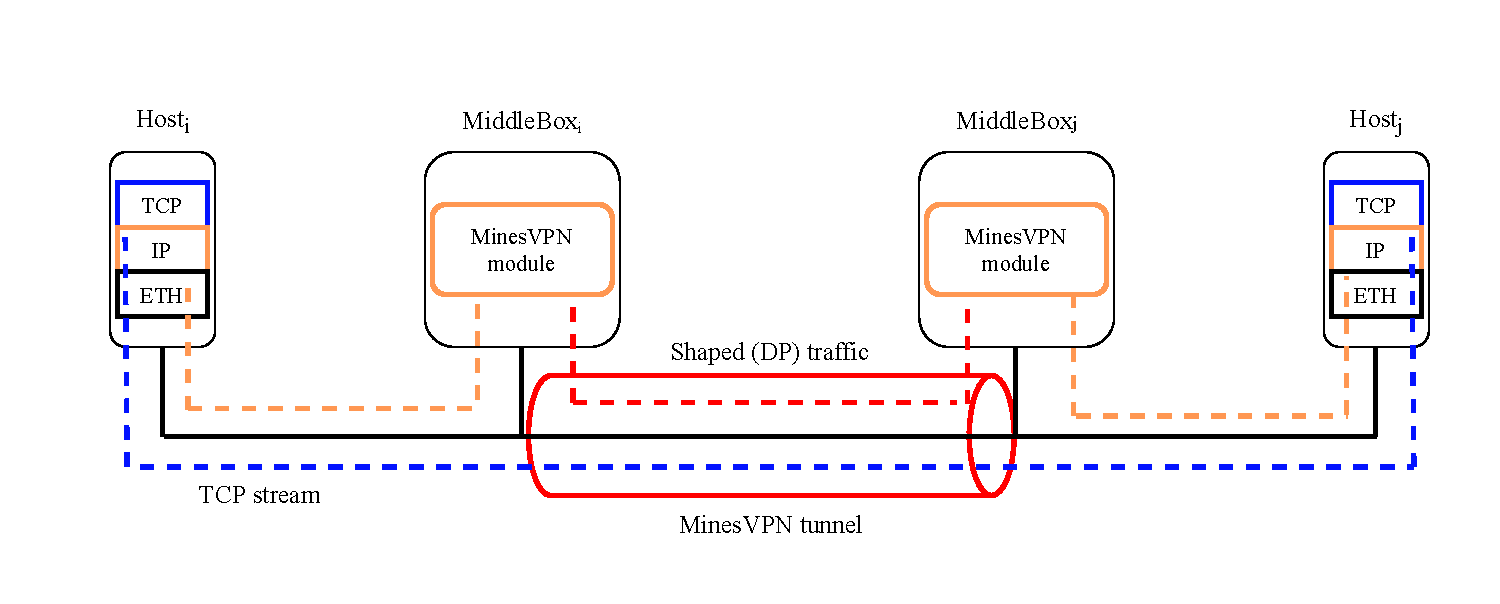
\includegraphics[width=\columnwidth]{figures/Design_highlevel.pdf}
%   %  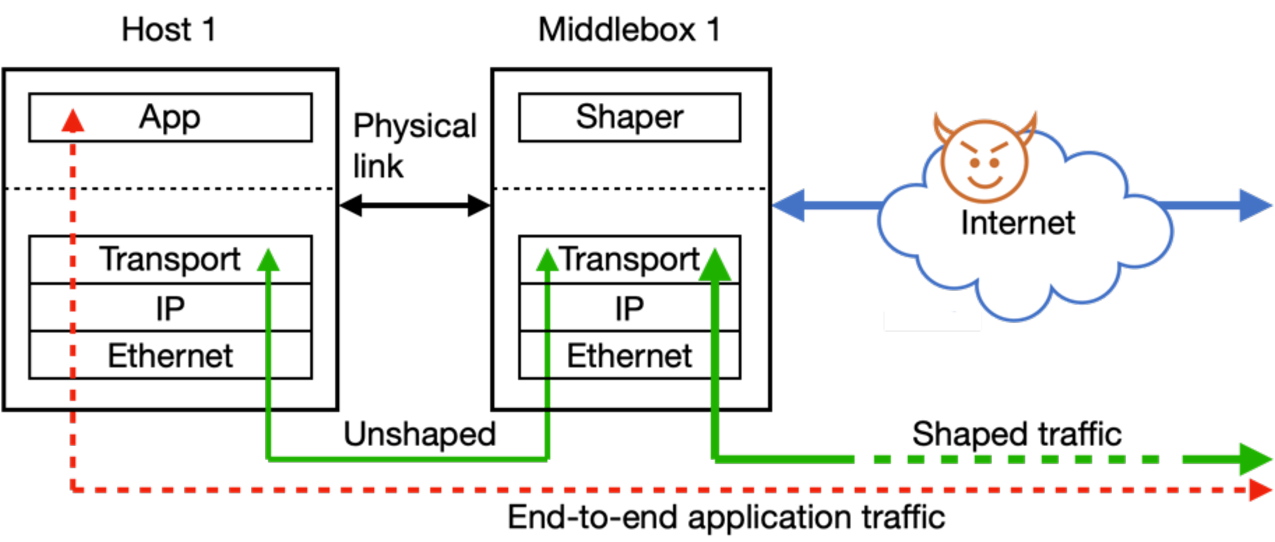
\includegraphics[width=\columnwidth]{figures/minesvpn-overview-half.pdf}
%   %  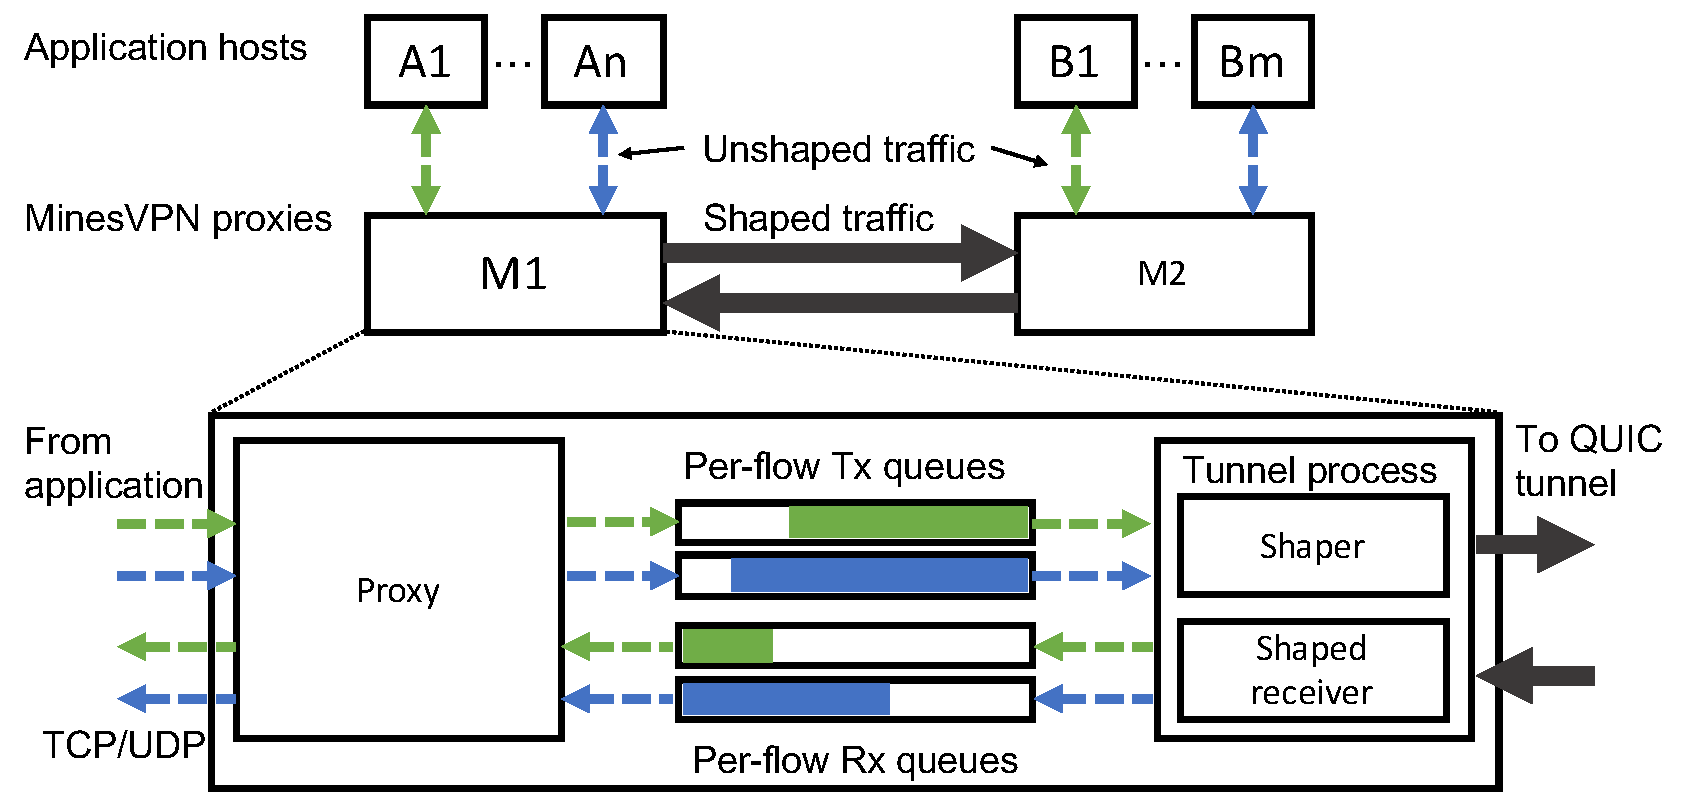
\includegraphics[width=\columnwidth]{figures/minesvpn-arch4.pdf}
%   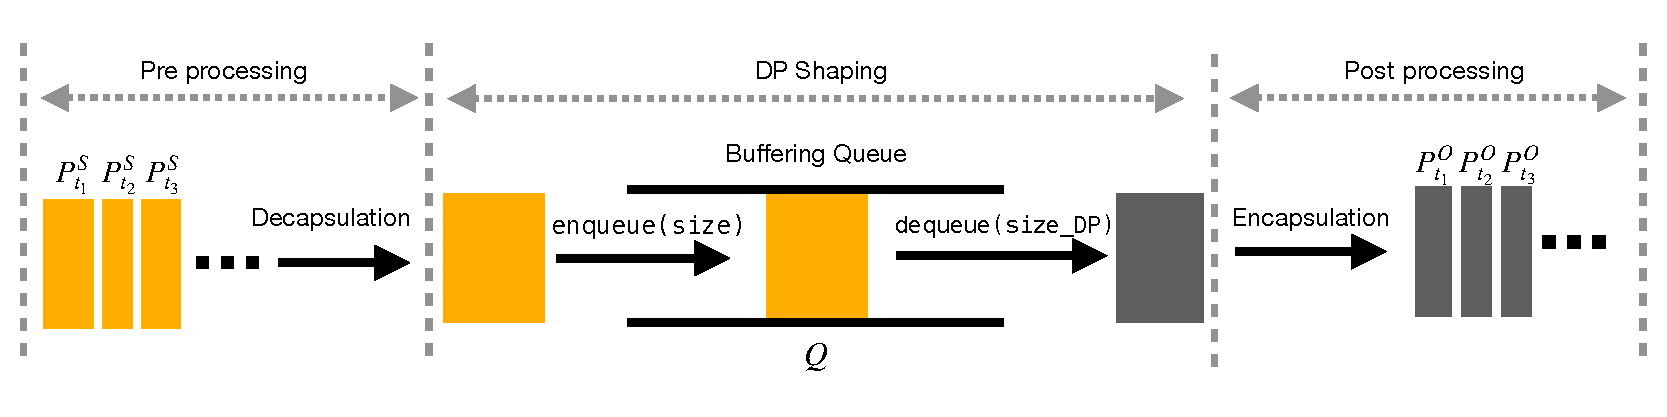
\includegraphics[width=\columnwidth]{figures/DPshaping_concept_horizontal.pdf}
%   \caption{{\sys} overview (one tunnel endpoint)
%       %\am{Update figure}
%   }
%   \label{fig:DPshaping_concept_horizontal}
% \end{figure}

\begin{figure}[t]
  \centering
  %  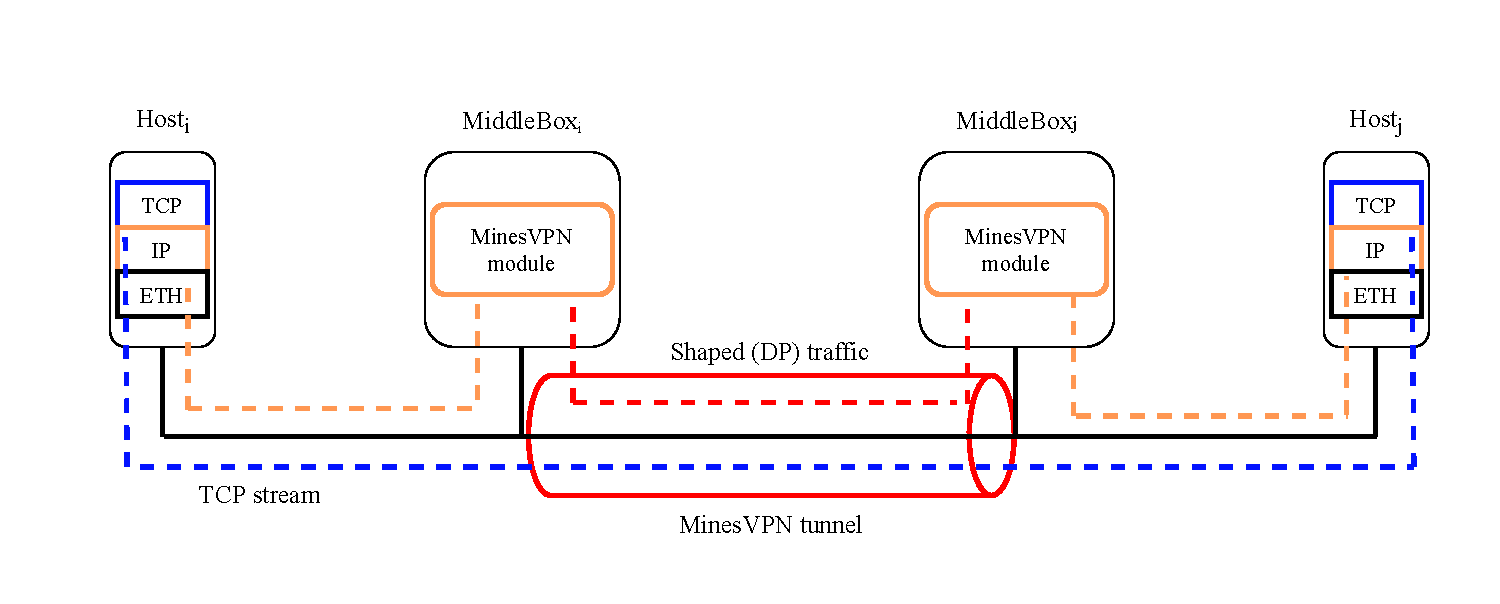
\includegraphics[width=\columnwidth]{figures/Design_highlevel.pdf}
  %  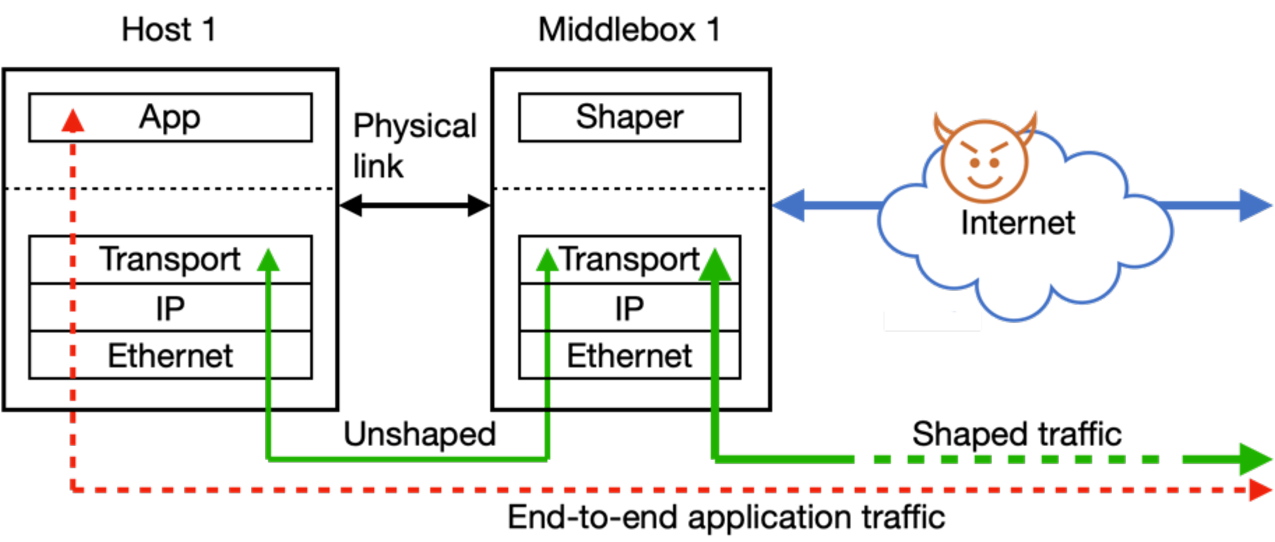
\includegraphics[width=\columnwidth]{figures/minesvpn-overview-half.pdf}
  %  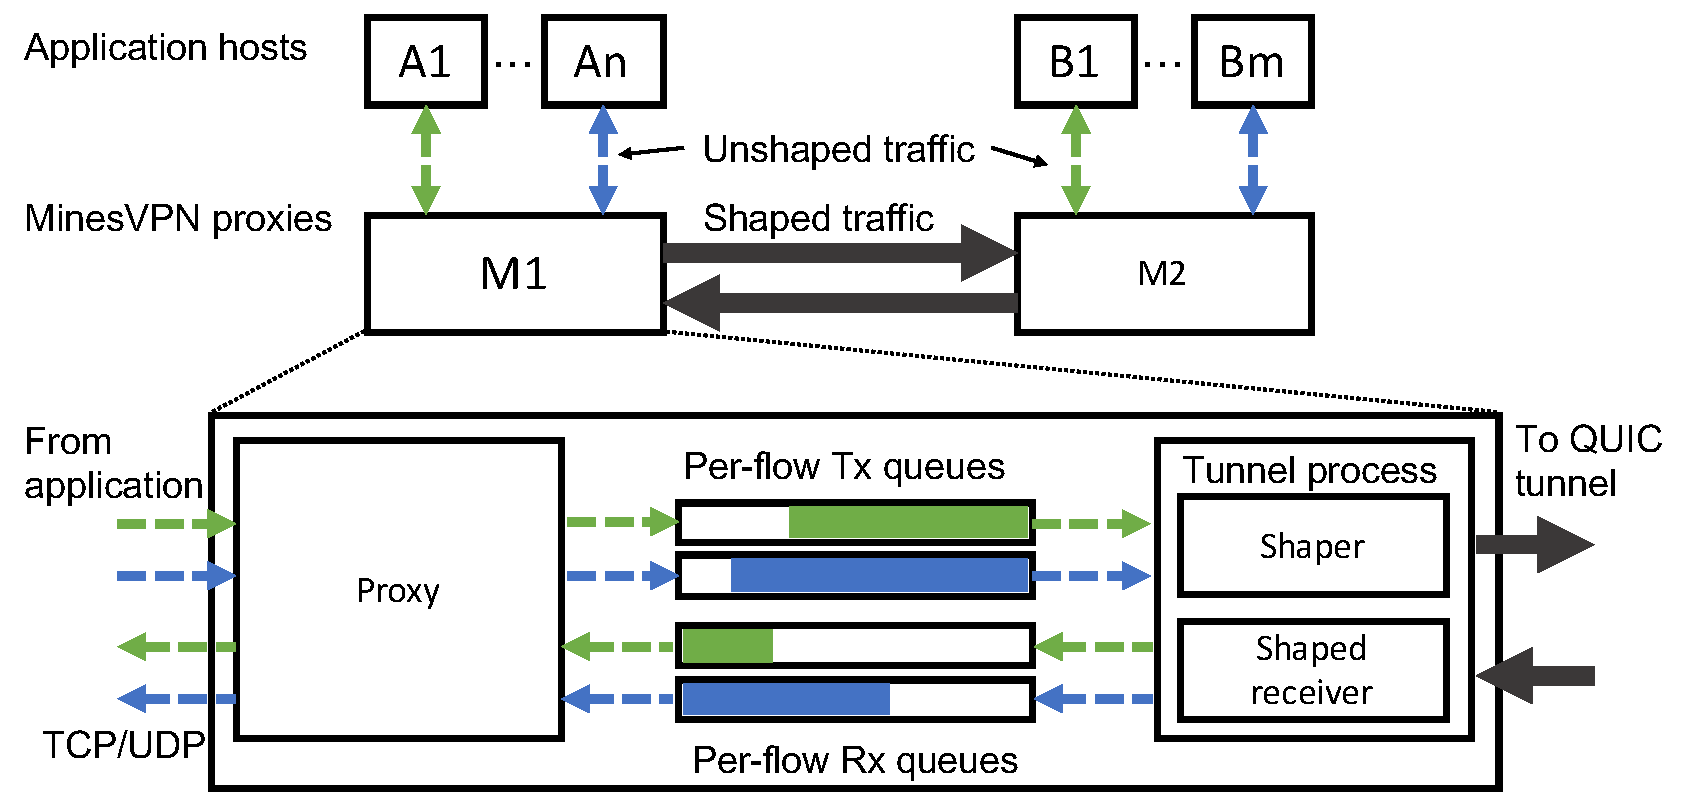
\includegraphics[width=\columnwidth]{figures/minesvpn-arch4.pdf}
  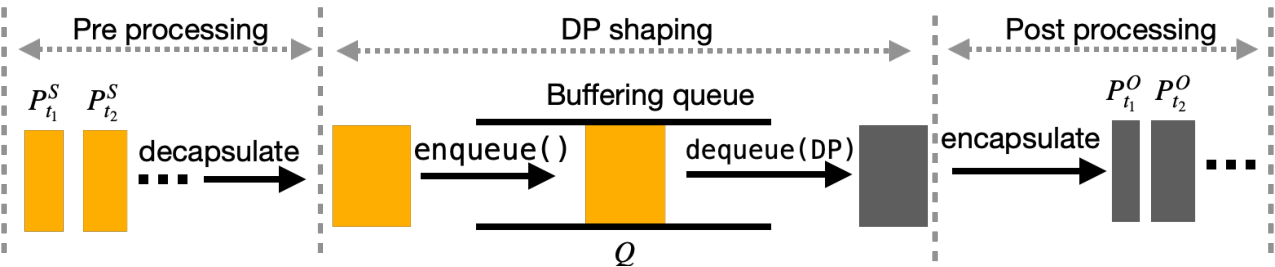
\includegraphics[width=\columnwidth]{figures/DPshaping_concept_vertical.pdf}
  \caption{{\sys} traffic shaping stages}
  \label{fig:DPshaping_concept_vertical}
\end{figure}

\subsection{DP shaping building blocks}
\label{subsec:infromation-bottleneck}
We define a source application stream $S$ (i.e. the input stream) as a sequence of packets:
\begin{equation}\label{equ:stream-pkts}
        S = \{P_{t_1}^S, P_{t_2}^S, P_{t_3}^S, \dots \} ,
\end{equation}
where $P_{t_i}^S$ is the size of the packet transmitted as a part of the stream
$S$ at the time $t_i$. \am{The symbol $S$ is overloaded in many places.}\as{all of them referring to the input stream}
%\am{I realize this model is inaccurate. A more accurate description is that an
%application byte stream is transformed into a sequence of packets. In absence of
%shaping, packet sizes and timing reveal the secrets. {\sys} transforms an {\em
%application byte stream} into a sequence of DP shaped bursts that are
%transmitted within fixed intervals. Basically, DP does not get an input as a
%packet stream but rather as a byte stream.}
%
Without {\sys}'s shaping, an eavesdropper can observe the entire stream:
$S = \{P_{t_1}^S, P_{t_2}^S, P_{t_3}^S, \dots \}$.
Typically, this information is strongly correlated with the data sent by the
application and the eavesdropper can infer sensitive information, such as the
specific video being sent by a streaming
application~\cite{schuster2017beautyburst}.


% We start by modeling an application stream in one direction as a
% dataset of packet sequences and by defining neighboring datasets from
% application streams.

% %\Cref{fig:minesvpn-arch} represents the abstracted design of the {\sys}
% %middle-box.  The incoming traffic in \Cref{fig:minesvpn-arch} is in form of
% %packets.  We formalize a stream of traffic, $S$, with the following
% %representation:

% %\smallksip\noindent
% \paragraph{Input stream.}
% We model an application stream, $S_I$ as a sequence of packets
% %$\{P_{t_1}^S, P_{t_2}^S, P_{t_3}^S, \dots \}$,

% \begin{equation}\label{equ:stream-pkts}
        % S_I = \{P_{t_1}^S, P_{t_2}^S, P_{t_3}^S, \dots \}
% \end{equation}
% where $P_{t_i}^S$ is the size of the packet transmitted as a part of the stream
% $S$ at the time $t_i$.

%leading to information leakage \cite{beautyburst} \todo{More
%references are needed}.
%{\sys}'s {\DPlogic} decides {\em how many bytes} of data to enqueue into DP
%queue and {\em when} to enqueue them, which we collectively call DP
%mechanism.

%\ml{\am{Aastha} I feel like the DP section would be easier to digest
%if it came after the design section.}
In {\sys}, we first introduce an information bottleneck in the form of a
buffering queue, {$\unshapedQ$}, to control the information accessible by an
eavesdropper. The buffering queue has three operations: \texttt{enqueue(size)},
\texttt{dequeue(size)}, \texttt{get\_size()}.
Conceptually, {\sys} decapsulates all application traffic of incoming stream $S$, and enqueues it in the {$\unshapedQ$}.
The shaping mechanism in {\sys} periodically retrieves the queue size and determines the amount of data to dequeue from $\unshapedQ$ in order to transmit it as shaped traffic.
The shaped traffic is encapsulated into a new sequence of packets, which we
denote as:
\begin{equation}\label{equ:stream-segs}
  O = \{P_{t_1}^O, P_{t_2}^O, P_{t_3}^O, \dots\}
\end{equation}
where $P_{t_i}^O$ is a packet sent in the shaped tunnel.

In order to ensure that the observable stream $O$ preserves the privacy of the
original stream $S$, {\sys} ensures that $O$ is Differentially Private.
To enforce DP, {\sys} ensures that any input to $O$ that depends on sensitive
data (the stream $S$) is measured with DP. \am{Are we using $O$ for anything
other than just referring to the output packet sequence in the text and in the
diagram? This notation does not seem necessary for the rest of the section.}
\as{O just refers to the output (DP) packet sequence both in text and in diagram. Mathias used the $O$ for the output packet sequence and I didn't change the notation. }
\Cref{fig:DPshaping_concept_vertical} shows the end-to-end traffic shaping of
{\sys}.
After decapsulating incoming packets, the incoming traffic is stored in a
buffering queue. In fixed periods of length $T$, the \texttt{dequeue} operation is performed,
ensuring that the timing of the outgoing traffic remains independent of the
incoming traffic. 
We refer to $T$ as the length of update interval.
The size of the \texttt{dequeue} is determined by our
differential privacy mechanism, guaranteeing that the size of the outgoing
traffic remains DP.
Furthermore, the encapsulation and packetization of outgoing data can be
characterized as a post-processing step of a differentially private mechanism,
and therefore is DP.



%\am{If we agree
%about the model from byte stream to packet stream (unshaped) and burst stream
%(shaped), then this section can simply go away. The notion of shaping byte
%stream into a DP burst stream is already mentioned in the paragraph ``Traffic
%shaping within a tunnel'' in \S\ref{subsec:design-overview} currently. The only
%remaining abstraction is that of the queue. Do we need to introduce that in
%\S\ref{subsec:design-overview}?}

%\ml{$\leftarrow$ section where we show our attacks}

% \paragraph{Observed stream.}
% We define an observed stream $S_O$ as a sequence of bursts
% %transmitted at intervals of $T$
% %$\{B_1^S, B_2^S, B_3^S, \dots\}$,
% \begin{equation}\label{equ:stream-segs}
  % S_O = \{B_1^S, B_2^S, B_3^S, \dots\}
% \end{equation}
% where $B_i^S = \sum_{t_j \in [T_{i-1}, T_i]} P_{t_j}^S$ is the amount of traffic
% received between time intervals $T_{(i-1)}$ and $T_i$.
% Here, $T$ determines the granularity of attacker's observation.
% In absence of traffic shaping, an attacker can observe $S_O$ with high
% granularity and, if $S_O$ is correlated with secrets, can infer the
% secret~\cite{beautyburst}.
% %Our differentially private traffic shaping strategy ensures that the attacker is
% %not able trace back any traffic pattern transmitted over a public network to its
% %original pattern. This is achieved by shaping the traffic stream such that any
% %neighboring set of traffic streams has an equal probability of producing the
% %observed pattern. We will elaborate on our definition of neighboring streams in
% %the next section.

\subsection{DP queue measurements}
\label{subsec:dp-queue-measurements}
We define the queue $\unshapedQ_{\tau}$ as the size of {$\unshapedQ$} at time $\tau$.
To measure $Q_\tau$ with $(\varepsilon, \delta)$-DP, {\sys} uses an additive Gaussian noise mechanism.
That is, it computes $\tilde{Q}_\tau \triangleq Q_\tau + z$, where the noise $z$
is sampled from a normal distribution with a variance that depends on the DP
parameters and the sensitivity $\Delta$: $z \sim \mathcal{N}\big(0, \sigma^2 =
\frac{2\Delta}{\varepsilon}\ln(\frac{1.25}{\delta})\big)$.
Intuitively, the sensitivity $\Delta$ represents the size of a change in traffic
against which we quantify DP guarantees. Combining all of these elements, \Cref{alg:dp_shaping_mechanism} presents a simple pseudo-code for traffic shaping in {\sys}.
% \begin{algorithm}[h]
%   \While{not at end of data transmission}
%   {
%       $\unshapedq_{\tau}$ = \texttt{get\_size()} \;
%       $\tilde{\unshapedQ}_{\tau}$ = $\unshapedQ_{\tau} + z$ \;
%       \texttt{dequeue($\tilde{\unshapedQ}_{\tau}$)} \;
%       \texttt{sleep($T$)}
%   }
%   \label{alg:dp_shaping}
%   \caption*{{\sys} traffic shaping}
% \end{algorithm}

\begin{algorithm}[t]
  \caption{{\sys} DP traffic shaping}
  \label{alg:dp_shaping_mechanism}
  \begin{algorithmic}[1]
  \While {\textbf{not} end of data transmission}
    \State $\tau$ = \texttt{current\_time()}
    %
    \State $\unshapedQ_{\tau}$ = \texttt{get\_size()}
    %
    \State $\tilde{\unshapedQ}_{\tau}$ = $\unshapedQ_{\tau} +
    \mathcal{N}\big(0, \frac{2\Delta}{\varepsilon}\ln(\frac{1.25}{\delta})\big)$ \;
    %
    \State \texttt{dequeue($\tilde{\unshapedQ}_{\tau}$)}
    \State \texttt{sleep($T$)}
  \EndWhile
  \end{algorithmic}
\end{algorithm}



As we can see, the Gaussian noise is scaled to $\Delta$, so protecting traffic
that can change by larger amounts requires more noise to be added.
In DP, the sensitivity $\Delta$ is defined as the worst-case change of our
measurement $Q_\tau$, when changing one stream going through {$\sys$}.
To formalize this notion, we first need to define what changing one stream means.
In DP, this is done through a neighboring definition, which defines the
protection unit for our DP mechanism:

\begin{definition}
\label{def:neighboring-streams}
Consider two streams, $S$ and $S'$, being transmitted within a window of duration $w_s$. We define them as neighbors if
\begin{equation}\label{equ:stream-neighboring}
  \|S_t - S'_t\|_1 \leq D_s \; (bytes)
\end{equation}
%\ml{we probably need $w_S$ here or something, as we now have a protection window
%by assumption/design or dropping queues without anything sent for too long, and
%a measurement window by assumption of length}
%\as{I think we can just mention the $w_s$ here as a requirement/assumption, and
%then in design section, we say we'll enforce this assumption by dropping the
%data after $w_s$ seconds. Dropping the data to me is more like a design decision
%as it is not the only option to enforce this requirement. In an "imaginary"
%scenario, we can assume applications terminate their connections after $w_s$
%seconds of delay and there is no need to assume that the traffic can
%accumulate.}:

\end{definition}

That is, $S$ and $S'$ are neighbors if the L1-norm of their difference is less than $D_s$ on the time window of size $w_s$ (both $D_s$ and $w_s$ are parameters).
%
We utilize the L1-norm as our distance metric to quantify the dissimilarity
between two traffic streams, as it captures differences in both segment size and
temporal pattern.
%
Intuitively, {$\sys$} aims to ensure that a stream $S$ is indistinguishable (in the DP
sense) from a neighboring stream $S'$ by observing the shaped traffic.

Based on \Cref{def:neighboring-streams}, we can define the sensitivity $\Delta$ as the maximum
difference in {$\unshapedQ$} size at any time, had we changed stream $S$ from
any neighboring stream $S'$:
\begin{equation}
  \Delta = \max_{\tau}\max_{S, S'} | Q_{\tau} - Q'_{\tau} | .
\end{equation}

A key feature of $\sys$'s design is to ensure that the amount of data in a queue
can only change by at most $D_s$ when changing a stream $S$ by a neighboring
$S'$. We elaborate on this in \Cref{sec:design}.
Formally, {$\sys$} offers the following guarantee:
\begin{proposition}\label{prop:sensitivity}
  {$\sys$} enforces $\Delta \leq D_s$.
\end{proposition}
\begin{proofsketch}
  The proof relies on the following properties of {$\sys$}.
  Within windows of $w_s$ seconds, if $Q'_{\tau} > Q_{\tau}$, for the same noise draw $z$, $\tilde{Q}'_{\tau} > \tilde{Q}_{\tau}$, and \Cref{alg:dp_shaping_mechanism} sends at least as much data under $Q'_{\tau}$ as under $Q_{\tau}$, but not more than $\tilde{Q}'_{\tau} - \tilde{Q}_{\tau}$.
  Hence, $|Q'_{\tau+1} - Q_{\tau+1}| \leq |Q'_{\tau} - Q_{\tau}|$ and queues only get closer by \Cref{alg:dp_shaping_mechanism}, and only grow apart by the difference between $S$ and $S'$.
  The formal proof is in Appendix \ref{appendix:dp}.
\end{proofsketch}

Therefore, the accumulated difference between $S$ and $S'$ is upper-bounded by $D_s$.
This bound on the sensitivity of {$\unshapedQ$} over neighboring streams enables {$\sys$} to provide $(\varepsilon_{w_s}, \delta_{w_s})$-DP guarantees for shaped traffic stream observed for a given time window $w_s$. Formally, we have that:
\begin{proposition}\label{prop:dp}
  {$\sys$} enforces $(\varepsilon_{w_s}, \delta_{w_s})$-DP, with
  $\varepsilon_{w_s}, \delta_{w_s} \triangleq \textrm{DP\_composition}(\varepsilon,
  \delta, \lceil\frac{w_s}{T}\rceil)$.
\end{proposition}
\begin{proof}
By \Cref{prop:sensitivity}, the sensitivity of one {$\unshapedQ$} is $\Delta$. Every $T$ seconds, by the Gaussian mechanism the observed queue size, $\tilde{\unshapedQ}_{\tau}$, is $(\varepsilon, \delta)$-DP.
Over a time period of length $w_s$, there are at most $\lceil\frac{w_s}{T}\rceil$ measurements taken. The proof is then concluded by applying DP composition.
\end{proof}

Given the privacy parameters, $\varepsilon$ and $\delta$, for one queue measurement, and the number of measurements, $\lceil\frac{w_s}{T}\rceil$, the  $\textrm{DP\_composition()}$ uses RDP composition to calculate the aggregated privacy loss, $\varepsilon_{w_s}$, and failure probability, $\delta_{w_s}$, for the time window of $w_s$.
If $w_s$ is larger than any traffic stream to protect, {$\sys$} enforces $(\varepsilon_{w_s}, \delta_{w_s})$-DP over all streams going through he shaped tunnel. Note that this does not depend on the number of streams: the overhead (noise added to measurements) is the same regardless of how many streams use the shaped tunnel.




% \paragraph{Unshaped queue.}
% We model an abstract queue, {$\unshapedQ$}, which holds the unshaped input byte
% stream of an application and supports two operations: enqueue and dequeue.

% \paragraph{Neighboring queue states.}
% We define the queue state, ${\unshapedQ}_{\tau}$, as the amount of traffic
% inside ${\unshapedQ}$ at time $\tau$. We call two queue states, ${\unshapedQ}_{\tau}$
% and ${\unshapedQ}'_{\tau}$, neighbor queue states if and only if we have:
% \begin{equation}\label{equ:queue-neighboring}
        % |{\unshapedQ}_{\tau} - {\unshapedQ}'_{\tau}| \leq D_q \;(bytes)
% \end{equation}
% where $D_q$ is a parameter in our system.


% \paragraph{Query function and sensitivity.}
% We define a query function on the queue state ${\unshapedQ}$,
% $f({\unshapedQ}_{\tau})$, as a function that returns the
% size of the queue at time ${\tau}$. The sensitivity of the function $f$ is given~by:
% \begin{equation}
% \Delta_1 f = \max_{Q, Q'} \| f(Q_{\tau}) - f(Q'_{\tau}) \|_1 =  \max_{Q, Q'} \| Q - Q' \|_1 = D_q
% \end{equation}
% Here, $\Delta_1 f$ captures the magnitude by which the size of queue can change
% from one stream to another.  In fact, {\sys}'s shaping strategy guarantees that
% the queue size cannot be accurately ascertained by an attacker.  At this point,
% we have all necessary building blocks to propose our differentially private
% shaping algorithm.

% \paragraph{From queues to traffic streams.}

% The definition presented in \Cref{equ:queue-neighboring} serves as a sufficient
% basis for designing our differentially private traffic shaping based on queue
% states.  However, in order to provide comprehensive privacy guarantees for
% internet applications, we extend this definition from queue states to
% streams of traffic.


% To reason about the privacy of traffic streams, we need to define neighboring
% streams (i.e. the minimal protection unit of each differentially private
% algorithm).  Two stream prefixes, $S_t$ and $S'_t$ (with the representation of
% \Cref{equ:stream-segs}), are neighbors if and only if:
% \begin{equation}\label{equ:stream-neighboring}
        % \|S_t - S'_t\|_1 \leq D_s \; (bytes)
% \end{equation}
% We utilize the L1-norm as our distance metric to quantify the dissimilarity
% between two traffic streams, as it captures differences in both
% segment size and temporal pattern.


% Our goal is to measure, and subsequently bound, the privacy loss of a traffic
% stream.
% Intuitively, an attacker's observation of a traffic stream can be interpreted as
% a series of differentially private queries on the segment sizes of original
% traffic pattern. \am{I find this intuition of an attacker issuing DP queries
% strange. To me, the attacker performs usual queries on a database whose
% underlying distribution has been made DP.}
% We claim that the privacy loss for a individual traffic stream shaped with our
% mechanism can be quantified by aggregating the privacy loss incurred at each
% measurement of the abstract queue size.
% The following statement provides a formal representation of this notion.


% \ml{Amir, please use real latex things for the Claim and Lemma. I'd also call the Lemma Proposition instead: Lemma is for general theoretical tools others might reuse and apply to other proofs).}
% \textbf{Claim}: The privacy loss of transmitting a traffic stream with the
% length of $w = kT$ through the {\sys} middle-box, is the composition of $k$
% queries on the queue state.
% \\
% To show that this claim is true, we only need to prove the following lemma.

% \textbf{Lemma}: Assume two neighboring traffic streams, $S_t$ and $S_t'$,
% transmitted through a middle-box with \Cref{alg:middle-box-all} as the shaping
% mechanism. If they both reshaped to the same traffic stream, $S_O$, then,  at
% any given time $\tau$, the queue states for neighboring streams are $D$-close.
% In other words we have:
% \begin{equation}\label{equ:composition_dp_section}
        % \forall \tau > 0 : |Q_{\tau} - Q_{\tau}'| \leq D
% \end{equation}
% where $D = \min(D_q, Q_{max})$. $D_q$ and $Q_{max}$ are the queue neighboring
% threshold and maximum buffer size of our middle box respectively.
% \am{I see no relation between $D_q$ and $D_s$.}

% This means the unshaped queues of these two streams are always neighbors
% according to the neighboring definition of \Cref{equ:queue-neighboring}.
% We prove the Lemma in \Cref{appendix:dp}.

% Here, we show how we can calculate privacy loss for a traffic stream.
% Assume two neighbor streams, $S_t$ and $S_t'$, reshaped to the same stream,
% $S_O$, by {\sys} middle-box. If we show the shaping mechanism by $M_s$, the
% privacy loss is:
% \begin{equation}\label{equ:privacy-loss}
  % \log\big(\frac{\Pr[M_s(S_t)=S_O]}{\Pr[M_s(S_t')=S_O]}\big) \leq \varepsilon_g
% \end{equation}
% Using the representation of \Cref{equ:stream-segs}, we have:

% \todo{Add the equation}

% The composition comes into the picture in the inequality \todo{Add ref} as the
% size of output at each round depends on the amount traffic enqueued into the
% ${\unshapedQ}$ and outputs of previous rounds of the mechanism, which both
% abstracted in the queue state.

\if 0
\subsection{DP shaping mechanism}
\label{subsec:dp-shaping}

\ml{I feel like this all belong to \am{design} with the DP call as a noisy black
box.} \am{Yes, this is covered in \S\ref{subsec:design-overview}.}

\Cref{alg:middle-box-all} represents the differentially private shaping
mechanism.  The algorithm is executed periodically with an interval of $T$
seconds.  Here, we explain one round of the algorithm.
\begin{enumerate}
  \item The DP mechanism reads the current size of the queue, $Q_t$.
  \item Then, it adds a noise from a Gaussian distribution with an average of
  zero and scale of ${\sigma}$ to the current size. The noisy measurement is
  represented by $D^S_t$ in the algorithm, and $\sigma$ is the parameter that
  determines the privacy loss of our mechanism.
  \item To avoid unpredictable behaviors such as the occurrence of negative
  values in the noisy measurement, we have incorporated a minimum and maximum
  size threshold for the noisy measurements, which are adjustable parameters
  within the algorithm.
  \item If $D^S_t > Q_t$, the data in {\unshapedQ} will be padded to $D^S_t$
  bytes and subsequently transmitted to the receiver.
  Conversely, if the size of the data in {\unshapedQ} is less than or equal to
  $D^S_t$, the entirety of the $D^S_t$ bytes will be sent.  In algorithm
  \ref{alg:middle-box-all}, the padding size and real data size are represented
  with $D^P_t$ and $D^R_t$ respectively.
\end{enumerate}
\fi

Our algorithm ensures that an attacker cannot trace the observed segment sizes
on the network back to the original traffic pattern.  Furthermore, due to the
periodic execution of the algorithm, the timings of segments are independent of the
original pattern.

\am{The proof of the DP guarantees of the algorithm is provided in the
appendix. Can we prove that constant timing intervals + differentially privacy
on size = differentially privacy on the overall traffic shape?}
\section{Differentially Private Traffic Shaping}
\label{sec:dp}

\begin{figure}[t]
    \centering
    %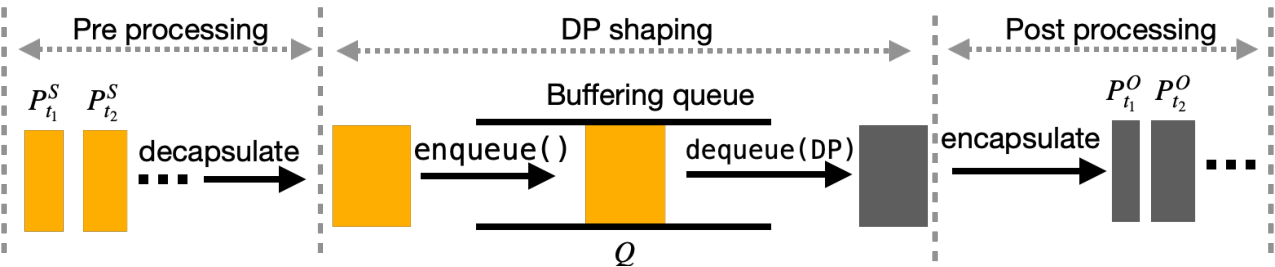
\includegraphics[width=\columnwidth]{figures/DPshaping_concept_vertical.pdf}
    %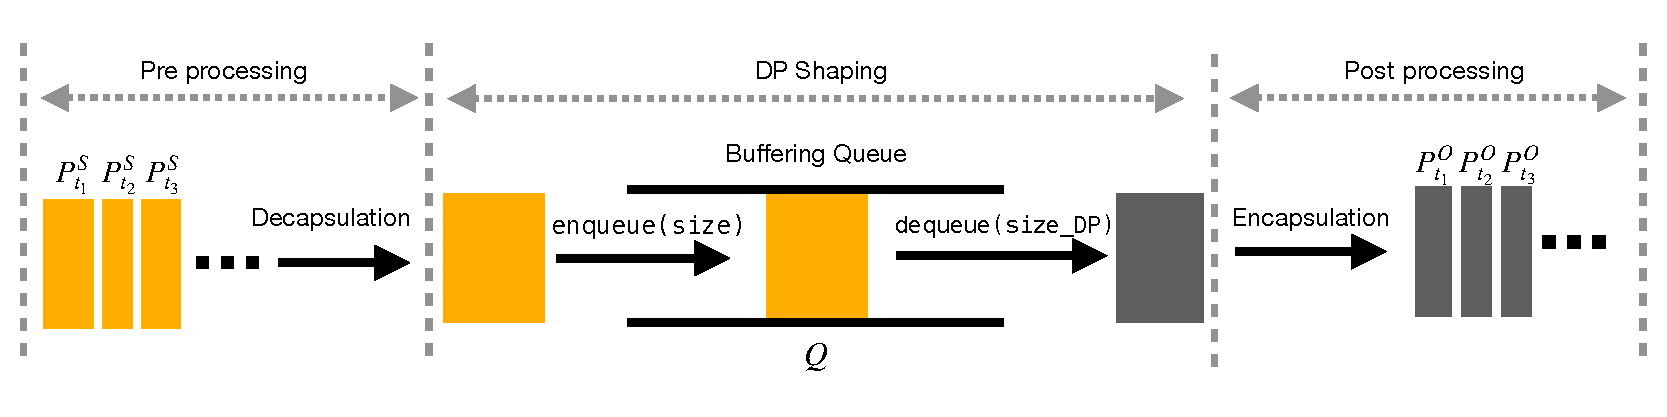
\includegraphics[width=\columnwidth]{figures/DPshaping_concept_horizontal.pdf}
    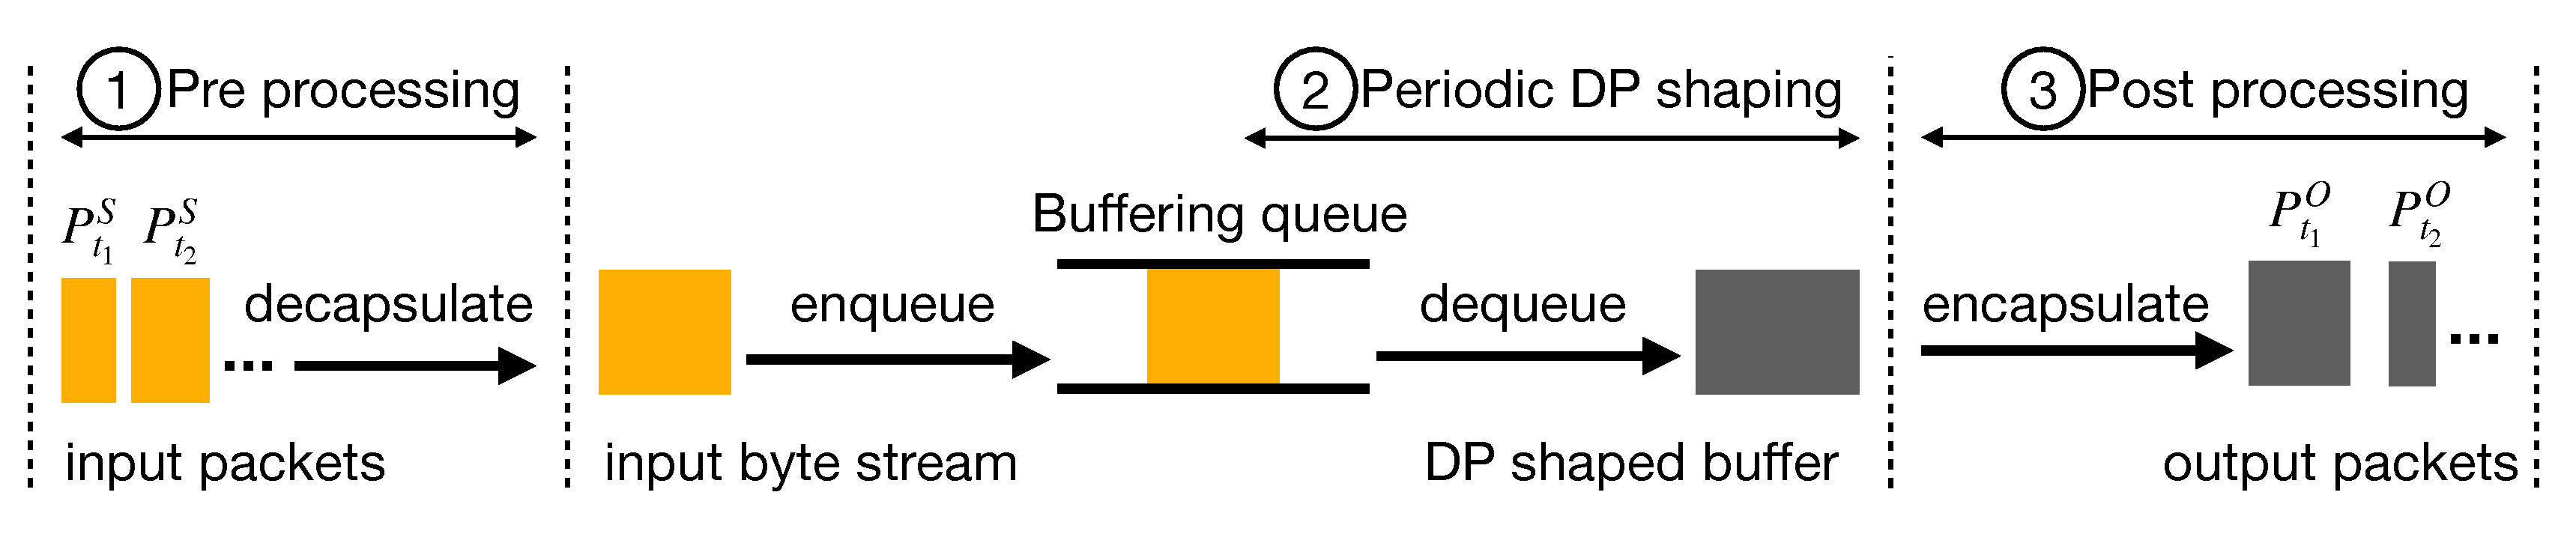
\includegraphics[width=\columnwidth]{dp-overview-fixed.pdf}
    \caption{Overview of DP shaping}
    \vspace{-0.4cm}
    \label{fig:dp-overview}
\end{figure}

The goal of differentially private shaping is to dynamically adjust packet
sizes and timing based on the available data stream, while ensuring that the DP
guarantees hold for any information that an adversary
(\S\ref{subsec:threat-model}) can observe.

%At a high level, \sys's DP shaping performs {\em DP measurements} of the amount
%of traffic to send, to adapt the shaped traffic size which preventing data
%leakage.
%
%To build the differentially-private shaping mechanism, we first define the
%``query'' on traffic streams that is subject to the DP mechanism. We call it a
%{\em DP measurement}, which measures the amount of application traffic available
%within a finite interval, adds noise to this amount according to the mechanism,
%and subsequently transmits a number of bytes equal to the noised amount.
%The DP shaping involves three steps (\Cref{fig:dp-overview}).
%First, the preprocessing step transforms an input stream $S$ over a window
%$\window$ into a byte stream, which is
%accumulated in a {\em buffering queue} $\unshapedQ$. (We denote the length of
%$\unshapedQ$ by $\qlen$.) Specifically, as application packets arrive, {\sys}
%extracts the payload bytes and enqueues them into $\unshapedQ$.
%\paragraph{Preliminaries.}
%\label{subsec:dp-preliminaries}
We first formally model an application's input stream as a packet sequence
$\istream = \{{P^{\istream}_1}, {P^{\istream}_2}, {P^{\istream}_3}, \dots \}$,
%{\as{why do we need a superscript here? it is already defined as $S$.}}
where ${P_i}^\istream = (l^{\istream}_i, t^{\istream}_i)$ indicates that the
$i$\textsuperscript{th} input packet in $\istream$ has length $l^{\istream}_i$
bytes and is transmitted at timestamp $t^{\istream}_i$.
We call the total duration of a finite stream $\streamduration^S
\triangleq \max t^{\istream}_i - t^{\istream}_1$.
%    \max t^{\istream}_i$.
%\am{We may need to address the boundaries of a single stream a bit more
%carefully. When a client starts streaming a video, what do we consider as the
%start time for the client-to-server stream? Is it the time of the first packet
%of the first segment request sent on the network or is it the time when the
%client ``clicked'' on a video to request it? Similarly, what do we consider as
%the start time for the server-to-client stream? Is it the time of the last
%packet of the segment request that generated the server response?}
%\ml{I don't know if we do need to address it all, but at least this is not the
%right place imh. Here we're talking about abstract streams, then one can decide
%to say "streams are when the button is clicked, and I compute if they're
%neighbors this way". Or am I missing something?}
Without shaping, an adversary can precisely observe $\istream$ and infer
the content, which is correlated with the~stream (\S\ref{subsec:attack-bg}).

%We assume that the finest granularities of packet sizes and timing that an
%adversary can observe are 1 byte and 1 ns, respectively.
%Thus, if $\istream$ has two consecutive packets as $(l_i, t_i)$ and $(l_j, t_j)$
%with $t_j = t_i + x$, then the adversary's effective observation between the two
%packets is $\{\cdots, l_i, 0_{(i+1)}, 0_{(i+2)}, \cdots, 0_{(i+x-1)}, l_j,
%0_{(i+x+1)}, \cdots\}$.
%We introduce this time granularity for clarity of explanation. We choose 1 ns as
%a reasonable time step that lets us observe individual packets in measurements,
%but a finer granularity can be swapped in without changing the guarantees.
%
%\update{
%For shaping, we define the primitive of a {\em buffering queue} $\buffQ$ to
%control the maximum amount of information subject to the DP mechanism and,
%hence, the sensitivity of the DP mechanism.
%}
%Conceptually, {\sys} extracts bytes from the input stream, $\istream$, and
%enqueues them in the buffering queue $\buffQ$.
%We denote the number of bytes present in $\buffQ$ (\ie length of the queue) by
%$\qlen$.

%\update{
%Additionally, we define a periodic interval, called a {\em DP measurement
%interval}, of length $\dpintvl$, which determines the frequency of applying the
%DP mechanism on traffic streams.
%For a DP measurement interval $[t_d,~t_d + \dpintvl)$ and a
%sub-sequence $\istream_d \subseteq \istream$ of the input stream that falls
%within the interval, \ie $\{P^{\istream}_i, \cdots P^{\istream}_j\}$ with
%$t^{\istream}_i \geq t_d$ and $t^{\istream}_j < t_d + \dpintvl$, the total
%application bytes accumulated in $\buffQ$ within the interval $\qlent{d} =
%\sum_{p=i}^{j} l^{\istream}_p$.
%}

\Cref{fig:dp-overview} provides a high-level overview of the
differentially-private shaping mechanism. Shaping happens in periodic intervals
of fixed length $\dpintvl$, called the {\em DP shaping intervals}.
\circled{1} As the packets in an application's stream arrive, the payload bytes
extracted from the packets are placed into a {\em buffering queue}, $\buffQ$.
\circled{2} In each periodic interval, the DP shaping algorithm
performs a {\em DP query}: it measures the length of $\buffQ$ with DP,
to determine the number of bytes to transmit in the next interval.
{\sys} then prepares a DP shaped buffer using the
payload bytes from $\buffQ$, and additional dummy bytes if required.
This shaped buffer is enqueued to be sent over the network at the end of
the DP shaping interval, right before the next interval starts.
\circled{3} Finally, data in the shaped buffer may be split into one or more
packets, as part of a post-processing step, and transmitted to the network.

The size of each shaped buffer generated in an interval has ($\varepsilon_{T},
\delta_{T}$)-DP guarantees. The per-interval guarantees
compose over a sequence of multiple intervals, thus providing DP guarantees for
traffic streams of arbitrary lengths. The guarantees degrade as the stream length increases (\Cref{prop:dp})

%We next elaborate on how this design enables \sys's formal DP guarantees.
%
We now discuss the steps of building a DP mechanism for
traffic streams in \S\ref{subsec:building-blocks} and the
%We show the complete differentially-private shaping workflow and discuss the
privacy guarantees in \S\ref{subsec:dp-queue-measurements}.
%Finally, we prove our guarantees in \S\ref{subsec:dp-proof}.

% \subsection{The Building Blocks}
% \label{subsec:infromation-bottleneck}

% \Cref{fig:dp-overview} illustrates {\sys}'s $(\epsilon,\delta)$-DP
% shaping strategy.
% %We denote an application's input packet sequence by
% An application's input stream is a packet sequence
% $\istream = {P^S_2}, {P^S_3}, \dots \}$,
% %{\as{why do we need a superscript here? it is already defined as $S$.}}
% where ${P_i}^S = (l^S_i, t^S_i)$ indicates that the $i$\textsuperscript{th} input
% packet in $S$ has length $l_i$ bytes and is transmitted at timestamp $t_i$.
% Without shaping, an adversary can precisely observe $\istream$ and infer
% the content,
% % which is any content that is correlated with this stream.
% which is correlated with the~stream~\cite{schuster2017beautyburst}.

%\paragraph{Goal.}
%The design of our traffic shaping algorithm relies on three key steps.
%The rest of this section is organized as follows.
%In \S\ref{subsec:infromation-bottleneck}, we formalize the information available
%to an attacker observing an application stream, which is the sequence of sizes,
%inter-packet intervals, and directions of packets at the finest granularity of
%observation.
%%We propose a primitive of a {\em buffering queue} to collapse all this
%%information into a sufficient statistic to adapt {\sys}'s transmission rate:
%%the
%%size of data in the queue waiting to be transmitted through our shaping
%%mechanism.
%%
%In \S\ref{subsec:dp-queue-measurements}, we describe our decision mechanism for
%sending data based on DP decisions.
%%We show how to perform {\em DP querys} of our buffering queue, in
%%order to adapt \sys's transmission rate with DP guarantees.
%%We show that under natural constraints on the transmission rate decision
%%mechanism, the change of queue size is bounded, allowing us to perform DP
%%measurements.
%%(\Cref{alg:dp_shaping_mechanism}).
%%Intuitively, we can use DP queue measurements and public information such as
%%network conditions to decide the amount of data to transmit.
%%Transmissions contain queued data when some is available, and dummy data
%%otherwise.
%%The stream observed by any attacker is a post-processing of the DP queries
%%issued on the queue (depends on the private data only through the DP
%%measurements), and is hence DP.
%%
%Finally, in \S\ref{subsec:dp-proof}, we provide a proof sketch for the DP
%guarantees of our shaping mechanism.

%{\as{I don't think we should summarize the intro of DP section into only one
%paragraph. We should give a summary of section here, explaining why we think DP
%shaping is a good idea and how it works Intuitively. More importantly, I think
%we need to  }}
%Specifically, given an application with a corpus of objects, the DP shaping
%ensures that each pair~of {\em neighbouring} objects---whose sizes are within a
%bounded distance---is indistinguishable under DP notion from the observations of
%their traffic shape.
%We denote the maximum distance between any pair of application objects by
%$\ssens$.
%
%Intuitively, {$\sys$} aims to ensure that a stream $S$ is indistinguishable (in
%the DP sense) from a neighboring stream $S'$ by observing the shaped traffic.

\subsection{DP for Traffic Streams}
\label{subsec:building-blocks}
% \subsection{The Sensitivity for DP Measurements}
% \label{subsec:sensitivity}

We now discuss the three steps for building a DP mechanism on
traffic streams. Specifically, we present our neighboring definition for
streams, define the DP query on streams that {\sys} runs and bounds its sensitivity,
and show the DP mechanism that we use to make the query DP.

%%%Defining neighboring streams on these sequences is challenging, since the
%%%lengths of different application streams as well as the packet sequences may
%%%have large variance, hiding which may require large amounts of noise. To bound
%%%this variance, we first transform an application's traffic stream into a {\em
%%%burst sequence}, i.e., a sequence of bursts transmitted in fixed-length
%%%intervals $\dpintvl$. Formally, we represent a burst sequence as: $\ibstream =
%%%\{{B^S_1}, {B^S_2}, {B^S_3}, \dots \}$, where ${B_i}^S = (L^S_i, i.\dpintvl)$
%%%indicates that the $i$\textsuperscript{th} burst in $S$ has length $L^S_i$
%%%bytes and is transmitted in the interval $i.\dpintvl$.

%The main primitive in \sys's DP adaptive shaping is a DP query of the
%buffering queue ($\buffQ$) size.
%As discussed in \S\ref{subsec:DP-background}, making a measurement DP requires
%three steps: defining a granularity of protection through a neighboring
%definition, bounding the sensitivity of the computation, and adding noise to the
%computation result.
%We describe the key ideas in \sys's design that make this possible.

\textbf{Step 1: Neighboring Definition.}
Building a DP mechanism requires a suitable definition of neighboring
streams, which requires a notion of distance between streams.
%Two streams are neighbors if their distance is below a configured threshold.
The neighboring definition has two implications. First, it
determines the sensitivity for a ``query'' subject to the DP mechanism and, in
turn, the amount of noise necessary for ensuring a given DP guarantee. Second,
it defines the granularity of privacy guarantee: intuitively, neighboring streams
are indistinguishable based on only the results of the DP mechanism applied to
them.
%\am{Is this about hiding between n and n+1 streams?}
%\ml{On really/only. It is n n+1 if your def covers the 0 stream. It is always
%about indistinguishability between two streams the are neighbors (ie you can't
%know if one or the other is running with high confidence---there's a discussion
%on that later for the DP semantics, towards the end. hopefully it makes it clear
%and we can remain high level here.)}
Hence, we aim for a neighboring definition for which ``streams have many
neighbors'', and the sensitivity of the DP query we want to run is as low as
possible.
%\am{We already discuss the two implications in the DP background in \S2.4. Is
%there a way to shorten this paragraph?}
%\ml{I think it's the first time we instantiate it for streams, so it seemed
%important to me. But I guess we can compact/delete if it's obvious and we
%need space?}
%\ml{should we use DP query instead of DP measurement?}

%\todo{
%Defining a distance over streams of arbitrary lengths would yield a weak
%neighboring definition, as differences accumulate over time.
%and all streams would be far from each other.
\update{Defining neighbors over streams has two challenges. First, the streams
can be arbitrarily long and the distance between streams would typically
increase with stream length. Secondly, if we consider streams with packet
timestamps at the finest granularity, the distance between the streams may be as
large as the sum of sizes of all packets in both streams. Both these factors
imply that a stream would either have few neighbors (enabling weak privacy), or
the neighboring definition would need to specify a large distance threshold,
requiring a lot of noise for strong DP guarantees.}
%\todo{Defining neighbors over streams of arbitrary lengths would be challenging,
%as the distance between streams would typically increase over time. As a result,
%a stream would either have few neighbors (weak privacy), or the neighboring
%definition would need to be based on a large distance threshold, requiring a lot
%of noise for strong DP guarantees.}
%}
% large values for sensitivity, which implies that shaping would require adding
% large amounts of noise to retain privacy.

To keep the neighboring distance threshold small, we take two steps.
First, we define the notion of a {\em neighboring window}, which is a time
interval of configurable length $\winlen$ over input streams.
For notational convenience, we set $\winlen$ as an integral multiple of the DP
shaping interval $\dpintvl$ and write
$\winlen = k \dpintvl$, although this is not a strict requirement.

%\ml{\sout{
%A finite sub-sequence $\istreamw \subseteq \istream$ that falls within the
%neighboring window is the packet sequence $\{P^{\istream}_i, \cdots
%P^{\istream}_j\}$ where $t^{\istream}_i \geq t_w$ and $t^{\istream}_j < t_w +
%\winlen$.
%}}
\update{Secondly, to measure the distance between streams over a neighboring
window, we consider the total bytes in each stream (burst lengths) transmitted
within coarse-grained time intervals and use the difference in the burst lengths
in the intervals within the window. Intuitively, we need an interval granularity
that is coarse enough to generate similar burst length sequences in more
streams, but is also small enough to bound the accumulation of differences over
time (to bound sensitivity, our next step).}
%\todo{
%We now need a notion of distance between two streams $\istream$ and
%$\istream'$ over a neighboring window $[t_w,~t_w +\winlen)$. To this end, we
%need to measure differences at a relevant granularity. Intuitively, we need a
%granularity that is coarse enough that differences between streams can average
%out, but small enough that we can later bound the accumulation of such
%differences over time (to bound sensitivity, our next step).
%%\am{I think the intuition for why we need the coarse granularity in the first
%place is not clear.}
%}
As will become clear with \Cref{prop:sensitivity}, the DP shaping
interval $\dpintvl$ is the coarsest granularity that we can use.
Hence, considering a neighboring window starting at a timestamp $t_w$, \ie
$[t_w,~t_w + \winlen)$,
we define the following representation of stream $\istream$ over the window
%Hence, we define the following representation of stream $\istream$ over a window
$[t_w,~t_w +\winlen)$ at granularity $\dpintvl$: $S_{t_w, W} = \{L^S_{t_w},
L^S_{t_w+\dpintvl}, L^S_{t_w+2\dpintvl}, \ldots, L^S_{t_w+(k-1)\dpintvl}\}$,
where $L^S_{t} \triangleq \sum_{(l^S_i, t^S_i) \in S} \1\{t^S_i \in [t,
t+\dpintvl)\} l^{\istream}_i$ is the total application bytes accumulated in
$\buffQ$ in the interval $[t, t+\dpintvl)$.

We now present the following neighboring definition:
\begin{definition}
\label{def:neighboring-streams}
Two streams $S$ and $S'$ are neighbors if, for any neighboring window
$[t_w,~t_w +\winlen)$, the L1-norm distance between their representations
$S_{t_w, W}$ and  $S'_{t_w, W}$  is less than $\ssens$.
Formally, $S$ and $S'$ are neighbors if:
\begin{equation}
\max_{t_w} {\norm{S_{t_w, W} - S'_{t_w, W}}}_1 \leq \ssens .
\end{equation}
\end{definition}
We utilize the L1-norm (the sum of absolute values) to quantify the distance
between two traffic streams, as it captures differences in both traffic size and
temporal alignment, at the granularity of $\dpintvl$.
%\ml{\sout{$\ssens$ is the maximum distance between neighboring streams and is
%computed as the max L1-norm of the difference between a pair of
%application
%streams in traffic bytes, over any neighboring window of length up to
%$\winlen$.}}
%
%
We will show (in \Cref{prop:sensitivity}) that despite our restriction
%\am{of defining neighboring streams over windows of at most length $\winlen$}
of defining neighboring streams at a granularity of $\dpintvl$, and of computing
distances over windows of length $\winlen$, we can quantify {\sys}'s DP
guarantees for streams at any granularity and of any length.
%\ml{maybe forward point to Prop 1, which doesn this?}

The neighboring window length $\winlen$ and neighboring distance
$\ssens$ are both configuration parameters, which are set before the start of an
application's transmission.
%\ml{
%%[[Note: moved.] I would move this entire discussion to the "Impact of DP
%%Shaping on Performance" header below. For now it is sufficient to know that
%%it's parameters and the order of magnitude I think. Later we can exlain how we
%%set it based on domain knowledge, and why, since we'll be ready to discuss
%%impact on perf.]
%In practice, setting $\winlen$ larger than $\streamduration_{max}$, the total
%length of the longest stream to be protected would yield $\ssens$ larger than
%the max distance of any stream pairs and incur unnecessary overheads.
%%and we require $\winlen \leq \streamduration_{max}$.
%On the other hand, the upper bound for $\ssens$ is the NIC's line rate times
%window length $\winlen$. While the upper bound value would ensure that all
%streams that can possibly be sent are neighbors with each other, yielding a
%strong DP guarantee and making any stream indistinguishable, it would also incur
%high overheads.
%%(\S\ref{}).
%%\am{Which section should we reference here?}
%%\ml{I don't know... I thought we evaluated the impact of W on overheads, but if
%%not we shouldn't ref anything}
%\todo{While smaller $\winlen$ implies smaller $\ssens$ (which would yield lower
%overheads) $\winlen$ is lower-bounded by the DP shaping interval $\dpintvl$,
%as will be clear in the subsequent paragraphs.}
%Typically, one would set $\winlen$ based on application
%domain knowledge, such as the fact that videos often consist of a sequence of
%segments requested at fixed intervals (\eg 5s) or the maximum size of a web
%request.
%}
In practice, $\winlen$ would be in the order of milliseconds to seconds.
Subsequently, one would determine $\ssens$ based on the typical
difference of traffic between application streams over windows of length
$\winlen$.
The practical upper bound for $\ssens$ is the NIC's line rate times
window length $\winlen$, but smaller values based on domain knowledge are
often possible.

\if 0
\paragraph{From windows to intervals.}
%\am{Add rationale for moving from $\winlen$ to $\dpintvl$.}
{Based on \Cref{assumption:window} and \Cref{def:neighboring-streams},}
the window length $\winlen$ affects the maximum number of bytes that can be
accumulated in the buffering queue (thus, the maximum distance between stream
pairs), as well as the transmission delay for the payload bytes enqueued.
Specifically, large windows lead to high-latency bursty traffic.
\shepherd{To reduce latency and burstiness}
\as{comment 1.b: we should explain how does having two windows reduce the
burstiness and why we cannot make W as small as T},
{\sys} further splits the neighboring windows into smaller intervals of length
$\dpintvl$, called the {\em DP shaping intervals}, and performs a {\em DP
measurement} at the beginning of each interval.
%
%The privacy loss over any window is now defined by applying DP composition
%on the privacy loss of intervals spanning the window.
%\ml{This is accurate, but would make way more sense (to me at least) as an
%    explanation/analysis {\bf after} we formally state the neighboring def, not
%    with definitions.}
\todo{Note that this quantization of application traffic into intervals is
essential for modeling the DP mechanism and the privacy, latency, and
bandwidth overheads. However, the model does not make any assumption about the
alignment of the actual traffic stream with the DP intervals.}
%Although an adversary can observe traffic at the finest granularities of packet
%sizes (\ie 1 byte) and timing (1 ns), we need to quantize the traffic to be able
%to model a DP mechanism as well as the privacy, latency, and bandwidth
%overheads.
\fi
%\update{At a high level, we have $\streamduration \geq \winlen > \dpintvl$. We
%    elaborate on parts of this relation later in this section.
%}

%\ml{This should go with the measurement. I think we should call it DP
%measurement and DP measurement interval in the overview, and then define it
%properly only when we actually define the measurement}
%Finally, we define the ``query'' on traffic streams that is subject to the DP
%mechanism. We call it a {\em DP measurement}, which measures the amount of
%application traffic available within a DP interval and adds noise to this amount
%according to the mechanism, to compute the number of bytes that must be
%transmitted in the interval. \am{Here or next subsection?}
%and subsequently transmits a number of bytes equal to the noised amount.

\textbf{Step 2: DP query and sensitivity.}
In {\sys}, a DP query measures the buffering queue length $\qlen$ with DP at
intervals $\dpintvl$. This noisy measurement determines the number of bytes
that must be transmitted in the interval.
%provide privacy guarantees.
To make the measurement of $\qlen$ differentially private, we need to bound the
sensitivity $\qsens$ of the queue length variable $\qlen$.
This sensitivity $\qsens$ is the maximum difference in $\qlen$ that can be
caused by changing one application stream to neighboring one. Formally, consider
two alternative neighboring streams $\istream$ and $\istream'$ passing through
the queue.
Suppose that when transmitting $\istream$ (similarly $\istream'$), the
queue length at time $k$ is denoted by $\qlent{k}$ (respectively $\qlent{k}'$).
Then, assuming w.l.o.g. that $k \geq k'$:
%\am{What does this assumption mean? That the two streams have
%different durations? Also, do we account for misaligned streams here?}
\setlength{\abovedisplayskip}{0pt}
\begin{equation}
    \qsens = \max_{k = 0}^{\streamduration}~\max_{\istream,
        \istream'} | \qlent{k} - \qlent{k}' |
    \label{eqn:ssens}
\end{equation}

Bounding $\qsens$ is still challenging though, as our neighboring definition
only bounds the difference in traffic between two streams over any window of
length upto $\winlen$.
Because of this, when $\streamduration >> \winlen$, differences between what
$\istream$ and $\istream'$ would enqueue in $\buffQ$ can accumulate over time,
and the difference betwen $\qlent{t}$ and $\qlent{t}'$ can grow unbounded over
time.
%\am{I don't fully understand the previous sentence. What does the neighboring
%streams definition and $\ssens$ have to do with the challenge of bounding
%$\qsens$.}\ml{is the above clearer now?}
% For long streams with $\streamduration >> \winlen$, differences between
% $\istream$ and $\istream'$ can accumulate and grow unbounded.

To bound $\qsens$, {\sys} relies on the key assumption that
the tunnel can always transmit all incoming data from
application streams within any $\winlen$-sized time window. That is,
%\ml{Is it the tunnel, or just the buffering queue?}
%\am{I think only the buffering queue needs to be able to flush the bytes, but t
    %is okay to be a little vague here.}
%In other words, we assume that:
%is that the tunnel can handle all incoming data from application streams within
%$\winlen$-sized window of time.
%Specifically, we make the following assumption:
\begin{assumption}\label{assumption:window}
All bytes enqueued prior to or at time $t$ are transmitted by time $t+W$.
\end{assumption}
%\ml{I'm making this more concrete as it's very useful for the discussion of W
%and T}
To enforce this assumption, {\sys} implements a time to live in the buffering
queue, flushing all bytes older than $\winlen$ from $\buffQ$ (see
\S\ref{sec:design} for more details).
%\ml{[Do we actually give these details? I didn't see it. Ideally we could add
%them, but if not let's just remove this sentence.]
%We give details about this tunnel design in \S\ref{sec:design}.}
%\am{In the eval section, we discuss values of $\winlen$ that simply satisfy our
%flushing requirement. Our system implementation and probably even design does
%not support it explicitly. I think we should say something in the design about
%tracking the expiry time of each byte in $\buffQ$ and then Shaper dropping
%expired bytes.}
%\ml{would make sense to me, but if we have space I guess?}
%\ml{Do we explain that somewhere? Should we actually explain it here (dropping
%the queues) so that we can discuss the $W$ and $T$ tradeoff in this section?}
%
Intuitively, this assumption caps the accumulation of traffic differences in
$\buffQ$ to the maximum difference over $\winlen$, \ie $\ssens$.
Since the size of $\buffQ$ cannot differ by more than $\ssens$ when changing a
stream by a neighboring one, the difference between DP query results of $\buffQ$
under two neighboring streams---which is the sensitivity of the DP query,
$\qsens$---is upper-bounded by $\ssens$. Formally:

\begin{proposition}\label{prop:sensitivity}
    {$\sys$} enforces $\qsens \leq \ssens$.
\end{proposition}

\begin{proofsketch}
Consider any two streams $\istream$ and $\istream'$, as in \Cref{eqn:ssens},
and any measurements time $k$.
The proof proceeds in two steps. First, under \Cref{assumption:window},
streams can accumulate queued traffic for at most {$\winlen$}, so two
different streams can create a difference $|\qlent{k} - \qlent{k}'|$ of at
most $\ssens$.
Second, dequeuing can only make two different queues closer: Consider
query time $k$, with queue lengths $\qlent{k} > \qlent{k}'$ (the
opposite case is symmetric).
For a DP noise draw $z$, we have $\qlendpt{k} > \qlendpt{k}'$. Since shaping
sends at least as much data under $\qlendpt{k}$ as under $\qlendpt{k}'$,
but no more than $\qlendpt{k} - \qlendpt{k}'$, after dequeuing we have
$|\qlent{k+1}' - \qlent{k+1}| \leq |\qlent{k}' - \qlent{k}|$.
In summary, the queue difference under two different streams
$\qsens$ can grow to at most $\ssens$ due to data queuing, and dequeuing only
decreases that difference, and hence $\qsens \leq \ssens$.  The complete
proof is in \S\ref{appendix:dp}.
\end{proofsketch}

% We can now reason about DP guarantees over intervals of length $\dpintvl$ in
% order to achieve the privacy loss for streams over longer transmission
% durations.
% We discuss this in \S\ref{subsec:dp-proof}.

%and we can bound the sensitivity of $\qsens \leq \ssens$.
%We defer the proof, which requires accounting for DP noise, to
%\S\ref{subsec:dp-proof}, Proposition~\ref{prop:sensitivity}.

%\ml{This shouldn't be here I think. We're talking about DP, and going from one
%measurement to many will be handled by composition in the next section. The
%discussion between $W$ and $T$ can happen at the end in the discussrion of the
%implications of our design for performance. I don't think it should be in the
%middle of this.}
%\am{Needs discussion?}

\if 0
\paragraph{Bounding Sensitivity.}
The second step in providing DP measurements is to bound the sensitivity of the
computation we want to make private. Remember that we aim to measure the state
of traffic to adapt the amount of shaped traffic we send.
Since the sensitivity is the worst case change in result between two neighboring
streams, we need to reason about the worst case change to any measurement we want
to make, when performing this measurement on two adjacent streams.
We defined adjacent streams in terms of the difference of amount of traffic sent
over time, but there could be large differences in packetization, making it
difficult to bound the impact on any measurement.
%
\sys's key idea is to use the primitive of a {\em buffering queue} to control
the maximum information accessible by a measurement, and hence the sensitivity
of the computation.
Conceptually, {\sys} extracts bytes from the input stream, $\istream$, and
enqueues them in the buffering queue $\buffQ$.
We denote the number of bytes present in $\buffQ$ (\ie length of the queue) by
$\qlen$.

With this primitive in place, we are now ready to define our DP measurement and
analyze its sensitivity. We use subscript $T$ to denote measurement specific
quantities.
As $\qlen$ is the amount of application data waiting in $\buffQ$ to be sent, we
would ideally want {\sys} to move $\qlen$ bytes from $\buffQ$ to the shaped
buffer, for it to be sent over the network.  Hence {\sys} measures $\qlen$, with
DP to provide privacy guarantees. To make the measurement DP we need to bound
$\qsens$, the sensitivity of $\qlen$, which is the maximum difference in the
queue length $\qlen$ that can be caused  by changing one application stream to
neighboring one.
Formally, consider two alternative neighboring streams $\istream$ and
$\istream'$ passing through the queue.
Suppose that when transmitting $\istream$ (similarly $\istream'$), the
queue length at time $t$ is denoted by $\qlent{t}$ (respectively $\qlent{t}'$).
Then, assuming without loss of generality that $\streamduration \geq
\streamduration'$:
\setlength{\abovedisplayskip}{0pt}
\begin{equation}
    \qsens = \max_{t = 0}^{\streamduration}~\max_{\istream,
        \istream'} | \qlent{t} - \qlent{t}' |
    \label{eqn:ssens}
\end{equation}

Bounding $\qsens$ is still challenging thought, as our neighboring definition
only bounds the difference in traffic between two streams over any window of
length $\winlen$.
For long streams with $\streamduration >> \winlen$, differences between
$\istream$ and $\istream'$ can accumulate and grow unbounded.
\fi

%To bound sensitivity, {\sys} relies on the key assumption that
%\todo{the tunnel can always transmit all incoming data from
%application streams within any $\winlen$-sized time window.}
%\ml{Is it the tunnel, or just the buffering queue?}
%In other words, we assume that:
%%is that the tunnel can handle all incoming data from application streams within
%%$\winlen$-sized window of time.
%%Specifically, we make the following assumption:
%\begin{assumption}\label{assumption:window}
%  All bytes enqueued \todo{prior to or} at time $t$ are transmitted by time
%  $t+W$.
%\end{assumption}
%We explain how to realize this assumption in a tunnel design in
%\S\ref{sec:design}.
%\ml{Do we explain that somewhere? Should we actually explain it here (dropping
%the queues) so that we can discuss the $W$ and $T$ tradeoff in this section?}
%%
%Intuitively, this assumption caps the accumulation of traffic differences in
%$\buffQ$ to the maximum difference over $\winlen$, and we can bound the
%sensitivity of $\qsens \leq \ssens$. We defer the proof, which requires
%accounting for DP noise, to \S\ref{subsec:dp-proof},
%Proposition~\ref{prop:sensitivity}.

\textbf{Step 3: Adding Noise.}
With sensitivity bounded at $\ssens$, we can now query $\qlen$ with DP using
an additive noise mechanism, which entails sampling noise $z$ from a DP
distribution and computing the DP buffer queue length as $\qlendpt{k} \triangleq
\qlent{k} + z$.
Specifically, {\sys} uses the Gaussian mechanism, in which
the noise $z$ is sampled from a centered normal distribution
$z \sim \mathcal{N}\big(\mu,~\sigma^2\big)$, where the variance is parameterized
by $\epsilon_\dpintvl$, $\delta_\dpintvl$, and~$\ssens$:
$\sigma^2 =
(2\ssens^2)/(\varepsilon_\dpintvl^2)\ln(1.25/\delta_\dpintvl)$.
%\frac{2\ssens^2}{\varepsilon_\dpintvl^2}\ln(\frac{1.25}{\delta_\dpintvl})$.
Parameters $\epsilon_\dpintvl$, $\delta_\dpintvl$ determine the amount of
noise added to each DP query~result.
%\ml{[Let's keep that for the proof.]\sout{Under this noise distribution, one
%measurement is \mbox{$(\epsilon_\dpintvl, \delta_\dpintvl)$-DP}.}}


\subsection{Privacy Analysis}
\label{subsec:dp-queue-measurements}

The previous section defines $(\varepsilon_{\dpintvl}, \delta_{\dpintvl})$-DP
guarantees for the traffic transmitted in an individual shaping interval. We now
discuss (i) the guarantees for longer
application streams, (ii) the guarantees on a packet-level sequence derived from
a shaped buffer sequence, and (iii) the privacy implications for streams that
fall outside of the neighboring definition.

\textbf{Guarantees for streams.}
Recall from the previous section that shaping happens at intervals
$\dpintvl$; in each interval we perform a DP query on the buffering queue length
$\qlen$ and create a shaped buffer of length $\qlendp$, which is subsequently
queued for transmitting over the network at the end of the interval.
%
%\ml{yeah maybe DP shaping interval is a better name for $\dpintvl$...}
Enqueueing data into the shaped buffer at the end of each shaping interval
creates a sequence of states for the shaped buffer $\{(\qlendp_1, T),
(\qlendp_2, 2T), (\qlendp_3, 3T), \dots \}$.
%\ml{can we get better notation for this?}
Although this sequence is not technically observable by an adversary, this is
where we prove our DP guarantees using DP composition over queries
performed during the stream transmission.
%while the stream is running (\S\ref{subsec:dp-proof}).

\begin{proposition}\label{prop:dp}
For any stream $\istream$ of duration $\streamduration^S \leq
\streamdurationcfg$, {$\sys$}
enforces $(\varepsilon, \delta)$-DP for the sequence $\{(\qlendp_1, T),
(\qlendp_2, 2T), (\qlendp_3, 3T), \dots \}$, with $\varepsilon, \delta
\triangleq \textrm{DP\_compose}(\varepsilon_T, \delta_T, \lceil
\frac{\streamdurationcfg}{\dpintvl} \rceil)$.
\end{proposition}

\begin{proof}
Consider two neighboring streams $\istream$ and $\istream'$. By design, the
times at which shaped buffers are queued are independent of application data, so
$\{(\qlendp'_1, T'), (\qlendp'_2, 2T'), (\qlendp'_3, 3T'), \dots \} =
\{(\qlendp_1, T), (\qlendp_2, 2T), (\qlendp_3, 3T), \dots \}$, and we can
restrict our considerations to the sequences $\{\qlendp_1, \qlendp_2, \qlendp_3,
\dots \}$ and $\{\qlendp'_1, \qlendp'_2, \qlendp'_3, \dots \}$.
By Prop. \ref{prop:sensitivity}, the sensitivity of each measurement is at most
 $\ssens$.
By the Gaussian DP mechanism, the measured queue size $\qlendp$ in each
interval is $(\varepsilon_{T}, \delta_{T})$-DP.
Using DP composition over the $\lceil \frac{\streamdurationcfg}{\dpintvl}
\rceil$ DP queries made during any duration $\streamdurationcfg$
%$(\varepsilon_{T}, \delta_{T})$-DP,
 yields the ($\varepsilon, \delta$)-DP guarantee.
\end{proof}
We use R\'enyi-DP composition on the Gaussian mechanism for
$\textrm{DP\_compose()}$. {\sys} provides a DP guarantee for streams of any
length $t$, with the guarantee degrading gracefully as DP composition (of
order $\sqrt{\streamdurationcfg}$ as the length grows).
%\am{broken sentence?}\ml{just forgot to close the parents}
%If $\winlen$ is larger than all traffic streams, {$\sys$} enforces
%$(\varepsilon_{\winlen}, \delta_{\winlen})$-DP over all streams going through he
%shaped tunnel. \am{Not sure what the previous statement is trying to
%say.}{\as{I also think maybe it is better to remove it}}

%\todo{Note that the overhead (\ie noise added) due to DP does not depend on the
%number of streams: the overhead is the same regardless of the number of streams
%transmitted through the buffering queue simultaneously.}
%\am{Organize it.}

\textbf{Guarantees for packet sequences.}
Data from the shaped buffer is sent over the network, and transmitted as a
packet sequence denoted by $\ostream = \{{P^O_1}, {P^O_2}, {P^O_3} \dots \}$.
These packets are a post-processing of the DP-shaped buffer. As long as the
packets are generated independently of any secret data, they preserve the
DP guarantees of shaping due to the post-processing property of DP.
This yields the following result, directly implied by \Cref{prop:dp}
and DP post-processing:
\begin{corollary}
\label{cor:dp}
For any stream $\istream$ of duration $\streamduration^S \leq
\streamdurationcfg$, {$\sys$}
enforces $(\varepsilon, \delta)$-DP for its output packet sequence
\ostream,
with $\varepsilon, \delta \triangleq \textrm{DP\_compose}(\varepsilon_T,
\delta_T, \lceil \frac{\streamdurationcfg}{\dpintvl} \rceil)$.
\end{corollary}

\textbf{Privacy for non-neighboring streams.}
%Finally, if two streams are not neighboring for the parameter $\ssens$, but with
Finally, if the distance between two streams is larger than $\ssens$, \eg say
$k\ssens$ for some factor $k$, {\sys} still provides a (degraded) DP guarantee
through group privacy \cite[Theorem 2.2]{dwork2014algorithmic} applied to the
Gaussian mechanism.
Namely, a DP query in each shaping interval $\dpintvl$ for the non-neighboring
stream provides $(k\epsilon_\dpintvl, \delta_\dpintvl)$-DP, and the guarantees
can be extended for the stream duration $\streamduration$ by applying DP
composition to this new value.


\textbf{Interpretation of the guarantees.}
\update{
%By buffering all data in a queue, and periodically deciding the size of
%the data to send over the network with a DP measurement,
\sys's shaping algorithm provides a ($\varepsilon_{\dpintvl},
\delta_{\dpintvl}$)-DP guarantee on the volume of application
traffic enqueued (in the buffering queue) in a fixed-length interval
(and, by post-processing, the volume of traffic observable on the network).
%The timing of shaped buffer enqueueing however is not protected by DP.
}
%This is why {\sys} enforces a constant timing for this queueing, at intervals
%of length $\dpintvl$.
%With such a constant timing, DP holds for all observable traffic, as shown in
%\Cref{prop:dp} and Corollary \ref{cor:dp}.
%\ml{is that the correct summary for timing?}
%\update{However, we note that this constant timing is enforced as a best effort
%due to our use of generic hardware, as detailed in \S\ref{}.}.
%
Under perfect timing for the DP shaping interval $\dpintvl$, the DP guarantee
ensures that two neighboring streams, \ie their contents, are indistinguishable
with the probability as defined in \Cref{eq:dp}. Smaller
$\varepsilon_{\dpintvl}$ and $\delta_{\dpintvl}$ implies higher noise in
shaping, which increases the uncertainty about the original stream in the shaped
traffic.
%(the lower $\epsilon$ and $\delta$, the higher the noise added and higher the
%uncertainty).
%Thus, an attacker cannot distinguish the content of stream from that of any
%neighboring stream.

%\update{Secondly, the DP guarantees are independent of the number of streams
%transmitted simultaneously through the buffering queue.}
%\am{\sout{Finally, if $\ssens$ is large enough for all streams to be neighbor
%with a stream that doesn't send any data, {\sys} also hides the presence of any
%one stream.
%%between the tunnel endpoints.
%Thus, an attacker cannot distinguish the number of streams with high
%precision, including whether zero or one streams are running.}}
%{Note that because the DP guarantees can be shared among all the streams
%multiplexed through the buffering queue simultaneously, the overhead (\ie
%noise added) due to DP gets amortized among the streams.}
%\ml{[Suggestion: Replace all above with from ``Secondly'' by:]
Secondly, to enforce the DP guarantees, the DP noise of the Gaussian
mechanism does not depend on the total number of flows. Intuitively, the DP
guarantee is shared among all the streams multiplexed through the buffering
queue simultaneously for a fixed amount of noise, and the overhead (\ie noise
added) gets amortized among the streams.
%}

%\begin{algorithm}
%\DontPrintSemicolon
%\caption{DP Shaping Mechanism
%    \am{Redundant}
%
%\KwIn{$Q_{DP}, Q_{dummy}$}
%\KwOut{$Q_{QUIC}$}
%
%\While{True}{
%%\texttt{sleep($T$)}\;
%%\texttt{enqueue($Q_{DP}, \{P_{t_1}^S, P_{t_2}^S, \dots\}$)}\;
%$\qlen$ = \texttt{len($Q_{DP}$)}\;
%$\qlendp$ =  \texttt{DP\_measurement($\qlen$)}\;
%$R$ = \texttt{$\min(\qlen, \qlendp)$}\;
%%$R$ = \texttt{dequeue($Q_{DP}, \min(\qlendp, \qlen)$)}\;
%$D$ = $\qlendp > R~?~\qlendp - R : 0$\;
%$outbuf$ = \texttt{dequeue($Q_{DP})$ + dequeue($Q_{dummy})$}\;
%\texttt{enqueue($Q_{QUIC}, outbuf$)}\;
%%$P_{t_1}^O, P_{t_2}^O, \dots $ = \texttt{QUIC\_send($Q_{QUIC}$)}
%}
%%\;
%\end{algorithm}

% \begin{figure}
%   \centering
%   \begin{minipage}{0.8\linewidth}
%     \begin{algorithm}H]
%       \caption{DP Shaping Mechanism}
%       \KwData{$P_{t_1}^S, P_{t_2}^S, \dots $}
%       \KwResult{$P_{t_1}^O, P_{t_2}^O, \dots $}

%       \While{True}{
%         \texttt{sleep($T$)}\;
%         \texttt{enqueue($Q_{DP}, \{P_{t_1}^S, P_{t_2}^S, \dots\}$)}\;
%         $\qlendp$ =  \texttt{DP\_measurement($Q_{DP}$)}\;
%         $R$ = \texttt{dequeue($Q_{DP}, \min(\qlendp, \qlen)$)}\;
%         $D$ = $\qlendp - R$\;
%         \texttt{enqueue($Q_{QUIC}, R + D$)}\;
%         $P_{t_1}^O, P_{t_2}^O, \dots $ = \texttt{QUIC\_send($Q_{QUIC}$)}}\;
%     \end{algorithm}
%   \end{minipage}
%   \caption{Description of the DP Shaping Mechanism}
% \end{figure}

\begin{figure}[t]
    \centering
    %  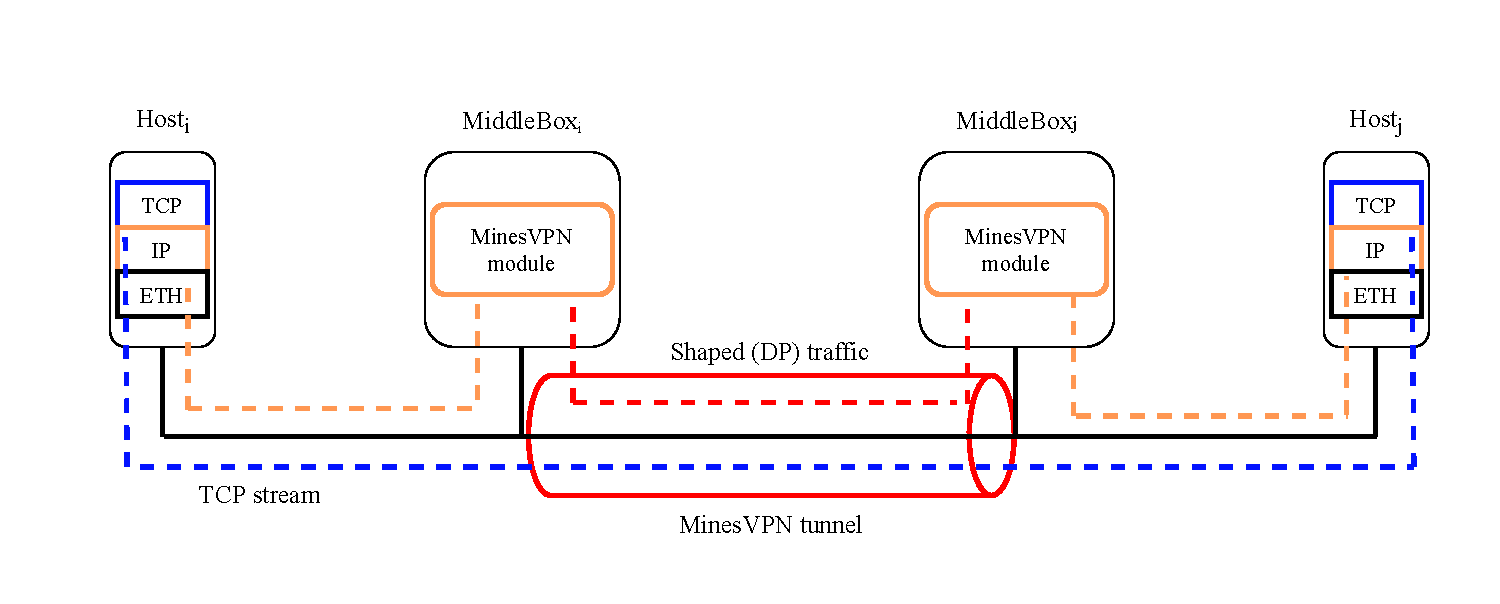
\includegraphics[width=\columnwidth]{figures/Design_highlevel.pdf}
    %  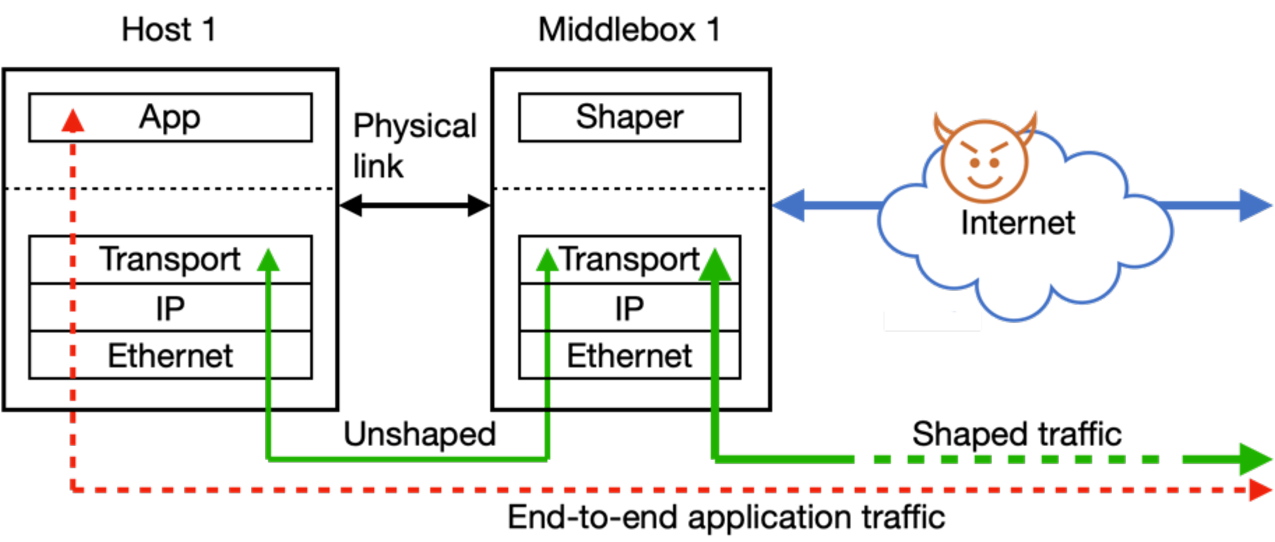
\includegraphics[width=\columnwidth]{figures/minesvpn-overview-half.pdf}
    %  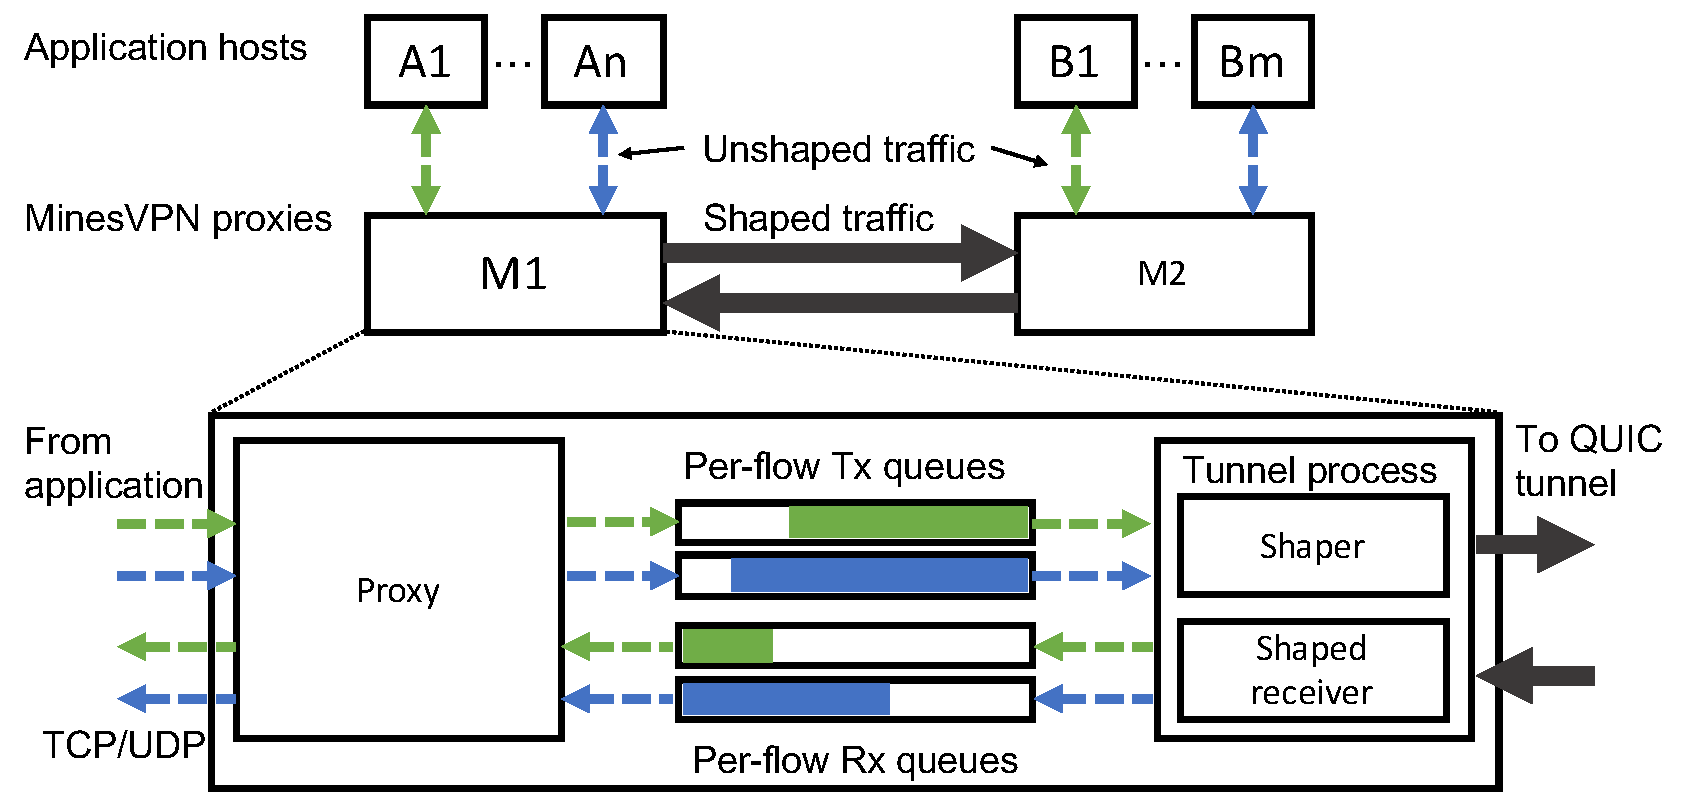
\includegraphics[width=\columnwidth]{figures/minesvpn-arch4.pdf}
    \includegraphics[width=\columnwidth]{design2.pdf}
    \caption{Overview of tunnel design (one endpoint)
        %\am{Update figure}
    }
    \vspace{-0.4cm}
    \label{fig:minesvpn-overview}
\end{figure}




\textbf{Privacy vs Performance.}
\sys's shaping mechanism introduces several parameters which impact privacy and
performance, specifically latency and bandwidth overheads. These parameters
include $\varepsilon_\dpintvl$, $\delta_\dpintvl$, $\ssens$, $\winlen$, and
$\dpintvl$.
%
%DP parameters $\ssens$, and ($\varepsilon_\dpintvl,
%\delta_\dpintvl)$ trade-off stronger privacy guarantees
%%(larger $\ssens$ strengthens the neighboring definition, and
%%$(\epsilon_\dpintvl, \delta_\dpintvl)$ the DP guarantee)
%for noisier measurements.
Larger $\ssens$ requires lower $\varepsilon_{\dpintvl}$ for stronger privacy,
which implies noisier measurements.
Noisy measurements imply more overhead---when the noise is positive, dummy bytes
need to be sent, incurring higher bandwidth overhead; when the noise is
negative, fewer bytes are sent and the unsent bytes accumulated in the buffering
queue incur a latency overhead.
This is the privacy-overhead trade-off we expect from DP.

Additionally, the parameters $\dpintvl$ and $\winlen$ have a more subtle impact
on the privacy-overhead trade-off.
%effect that also impacts the privacy-performance trade-off.
Traffic is shaped in intervals of $\dpintvl$; thus, $\dpintvl$ impacts the
latency and burstiness of the traffic.
A smaller $\dpintvl$ provides lower transmission latency and smaller bursts per
interval. However, it also requires more DP queries and, thus, incurs higher
privacy loss when transmitting the complete stream of a given length
$\streamduration$.
In practice, one would set $\dpintvl$ to the maximum value that can minimize
privacy loss while providing tolerable latency.

%$\winlen$ has a symmetric effect on privacy: a larger $\winlen$ for a fixed
%\todo{A practical upper bound for $\winlen$ is $\streamduration_{max}$, the
%total length of the longest stream in the neighboring set to be protected;
%$\winlen > \streamduration_{max}$ would yield $\ssens$ larger
%than the max distance of any stream pairs and incur unnecessary overheads.
%}
%On the other hand,
A large $\winlen$ for a fixed $\ssens$ implies that
neighboring streams can differ by at most $\ssens$ over a longer window size
$\winlen$, which weakens the neighboring definition and, hence, the privacy
guarantees.
%One would thus be tempted to make $\winlen$ as small as possible, maybe as small
%as $\dpintvl$.
While smaller $\winlen$ is desirable, the lower bound is $\dpintvl$.
Recall that, to bound $\qsens$ (\Cref{assumption:window}),
{\sys} must drop any bytes left in the buffering queue for longer than $\winlen$.
%older than $\winlen$ from the buffering queue.
Since data leaves the buffering queue in each shaping interval after a
DP query, setting $\winlen = \dpintvl$ would lead to immediate dropping of the
bytes from the buffering queue that aren't transmitted in response to the
DP query. This would happen \update{in each interval where the DP query samples
a negative noise value}.
%\am{for the first time?}\ml{no I mean "every time" here, is there a better way
%to say it?}.
These data drops would degrade {\sys}'s performance in terms of both
throughput and latency. Hence, we need $\winlen >> \dpintvl$ to ensure that data
has time to leave the buffering queue before it is too old.
Typically, one would set $\winlen$ based on application domain knowledge, such
as the maximum size of a web request or the fact that videos often consist of a
sequence of segments requested at 5s intervals.

We analyze the impact of different choices for these parameters on
the privacy guarantees and overheads in \S\ref{sec:eval}.

%\ml{Let's make sure this discussion addresses this at least:}
%\shepherd{To reduce latency and burstiness}\as{comment 1.b: we should explain
%how does having two windows recduce the burstiness and why we cannot make W as
%small as T}


\if 0

Specifically, large windows lead to high-latency bursty traffic.
\shepherd{To reduce latency and burstiness}\as{comment 1.b: we should explain how does having two windows recduce the burstiness and why we cannot make W as small as T}

\ml{[TODO: with at least this info taken from other places while moving things]
%
, {\sys} further splits windows into
smaller intervals of length $\dpintvl$ and samples noise at the beginning of
each interval.
\todo{Note that this quantization of application traffic into intervals is
essential for modeling the DP mechanism and the privacy, latency, and
bandwidth overheads. However, the model does not make any assumption about the
alignment of the actual traffic stream with the DP intervals.}
%\todo{In absence of shaping, the queue length corresponds to the amount of
%    unshaped traffic transmitted in an interval of $\dpintvl$.}
The privacy loss over a window is now defined by applying DP composition
on the privacy loss of individual intervals.
\am{Should the text from the beginning of this paragraph until the previous
sentence appear earlier as a justification for why we have separate $\winlen$
and $\dpintvl$?}
%
The privacy loss ($\varepsilon_{\winlen}$) and bandwidth overheads of the DP
shaping (represented by $\sigma_\dpintvl$, \ie the standard deviation of the
noise distribution function) depend on
$\winlen$, $\ssens$,
%$\varepsilon_{\dpintvl}$, $\delta_{\dpintvl}$,
and the number of intervals $\varnumupdates = \numupdates$ in $\winlen$.
Additionally, the latency overheads depend on $\dpintvl$.
Note that for a specific value of $\ssens$ and $\varnumupdates$, the DP guarantee
$\varepsilon_{\winlen}$ is fully specified by $\sigma_\dpintvl$, and remains the same even at
different time scales.
That is, scaling $\winlen$ and $\dpintvl$ proportionally does not change the
privacy and overhead costs.
%{\as{We are not sure about this, the latency can be affected by the amount of
%noise in extreme scenarios}}
}
\ml{[moved from above when I suggested removing]
In practice, setting $\winlen$ larger than $\streamduration_{max}$, the total
length of the longest stream to be protected would yield $\ssens$ larger than
the max distance of any stream pairs and incur unnecessary overheads.
%and we require $\winlen \leq \streamduration_{max}$.
On the other hand, the upper bound for $\ssens$ is the NIC's line rate times
window length $\winlen$. While the upper bound value would ensure that all
streams that can possibly be sent are neighbors with each other, yielding a
strong DP guarantee and making any stream indistinguishable, it would also incur
high overheads (\S\ref{}).
\am{Which section should we reference here?}
\ml{I don't know... I thought we evaluated the impact of W on overheads, but if
not we shouldn't ref anything}
\todo{While smaller $\winlen$ implies smaller $\ssens$ (which would yield lower
overheads) $\winlen$ is lower-bounded by the DP shaping interval $\dpintvl$,
as will be clear in the subsequent paragraphs.}
Typically, one would set $\winlen$ based on application
domain knowledge, such as the fact that videos often consist of a sequence of
segments requested at fixed intervals (\eg 5s) or the maximum size of a web
request.
}

\fi



\if 0
\subsection{Privacy Guarantees}
\label{subsec:dp-proof}
{\sys} provides ($\varepsilon_{\dpintvl}, \delta_{\dpintvl}$)-DP guarantees for
each DP measurement interval. Using this guarantee, one can then reason about DP
guarantees over a sequence of multiple intervals using DP composition methods.
In particular, for a transmission duration of length $D$, which consists of
$\lceil \frac{D}{\dpintvl} \rceil$ DP shaping intervals, {\sys} would provide
($\varepsilon_{D}, \delta_{D}$)-DP, with $\varepsilon_{D}, \delta_{D} \triangleq
DP\_compose(\varepsilon_{\dpintvl}, \delta_{\dpintvl}, \lceil \frac{D}{\dpintvl}
\rceil)$. We use R\'enyi-DP composition on the Gaussian mechanism for
$\textrm{DP\_compose()}$.
\am{Does this require proof?}

\if 0
%\as{I think we need to change the title of this section as it is not the proof
%but also proposing our guarantees. I suggest the title: "Privacy guarantees".}
At a high level, analyzing the  ($\varepsilon_{\winlen}, \delta_{\winlen}$)-DP
guarantee of the overall shaping mechanism requires two steps: (i) showing that
the difference in the buffering queue length is bounded for neighboring streams
for all transmissions of the streams (Prop. \ref{prop:sensitivity}), and (ii)
composing the DP cost of each measurement over the intervals defining a window
of length $\winlen$ (Prop. \ref{prop:dp}).
%\todo{(i) two neighboring streams in windows of length $\winlen$ are neighbors
%during all transmit intervals of length $\dpintvl$, and (ii) the total privacy
%loss composed over all transmit intervals within a window amounts to the privacy
%loss defined over the entire window.}
%\am{Verify wording.}
%\as{I think the wording is wrong for both points. We need to show that
%difference in queue lengths are bounded. Then the second point naturally follows
%by composition.}
%(i) the neighboring definition over the buffering queue length over intervals
%$\dpintvl$ implies neighboring definition

%Formally, {$\sys$} offers the following guarantee:
We first show that the sensitivity of each measurement $\qsens$ is at most the
window sensitivity $\ssens$:
\begin{proposition}\label{prop:sensitivity}
    {$\sys$} enforces $\qsens \leq \ssens$.
\end{proposition}

\begin{proofsketch}
  Consider any two streams $S_j$ and $S_j'$, as in \Cref{eqn:ssens}.
  The proof proceeds in two steps. First, under \Cref{assumption:window},
  streams can accumulate queued traffic for at most {$\winlen$}, so two
  different streams can create a difference $|\qlent{k} - \qlent{k}'|$ of at
  most $\ssens$.
  Second, dequeuing can only make two different queues closer: Consider
  measurement time $k$, with queue lengths $\qlent{k} > \qlent{k}'$ (the
  opposite case is symmetric).
  For a DP noise draw $z$, we have $\qlendpt{k} > \qlendpt{k}'$. Since shaping
  sends at least as much data under $\qlendpt{k}$ as under $\qlendpt{k}'$,
  but no more than $\qlendpt{k} - \qlendpt{k}'$, after dequeuing we have
  $|\qlent{k+1}' - \qlent{k+1}| \leq |\qlent{k}' - \qlent{k}|$.
  In summary, the maximum queue difference under two different streams
  $\qsens$ can grow to at most $\ssens$ due to data queuing, and dequeuing only
  decreases that difference, and hence $\qsens \leq \ssens$.  The complete proof
  is in \S\ref{appendix:dp}.
\end{proofsketch}

We can then reason about DP guarantees over intervals of length $\dpintvl$ in
order to achieve the privacy loss for the entire window of length $\winlen$.
%
\ml{[TODO Mathias] make notation consistent: here we want only the stream length
and then use W as a numerical application. This will show that we can compose over time}
Formally, we have:
\begin{proposition}\label{prop:dp}
  {$\sys$} enforces $(\varepsilon_{\winlen}, \delta_{\winlen})$-DP, with
  $\varepsilon_{\winlen}, \delta_{\winlen} \triangleq
  \textrm{DP\_compose}(\varepsilon_T, \delta_T, \numupdates)$.
\end{proposition}

\begin{proof}
By Prop. \ref{prop:sensitivity}, the sensitivity of each measurement is at most
  $\ssens$.
%\am{I thought the sensitivity is already defined in \Cref{eqn:ssens}.}
By the Gaussian DP mechanism, the measured queue size $\qlendpt{k}$ in each
interval $k$ of length $\dpintvl$ is $(\varepsilon_{T}, \delta_{T})$-DP.
% Over a time window of length $\winlen$, {\sys} will sample noise
% $\numupdates$ times.
Using DP composition over $\numupdates$ $(\varepsilon_{T}, \delta_{T})$-DP
measurements, and the fact that $\ostream$ is a post-processing of DP
measurements, yields the ($\varepsilon_{\winlen}, \delta_{\winlen}$)-DP over
any $\winlen$ length window.
% By using R\'enyi algorithm for DP\_compose(), we get $\varepsilon$,
% $\delta$ that correspond to ($\varepsilon_{\winlen}, \delta_{\winlen}$)-DP
% definition over $\winlen$ windows.
%\todo{Thus, the proof concludes with the application of DP composition.}
%\am{I am not sure how the last line follows from the second last line: what does
%it mean say proof concludes with application of DP composition.}
%\as{It is just the way of saying that compositions is applied here and privacy
%parameters, $\varepsilon_W, \delta_W$ are result of it.}
\end{proof}
We use R\'enyi-DP composition on the Gaussian mechanism for
$\textrm{DP\_compose()}$.
%If $\winlen$ is larger than all traffic streams, {$\sys$} enforces
%$(\varepsilon_{\winlen}, \delta_{\winlen})$-DP over all streams going through he
%shaped tunnel. \am{Not sure what the previous statement is trying to
%say.}{\as{I also think maybe it is better to remove it}}
Note that the overhead (\ie noise added) due to
DP does not depend on the number of streams: the overhead is the same regardless
of the number of streams transmitted through the buffering queue simultaneously.
\fi


%\smallskip\noindent
\paragraph{Summary.}
By buffering all data in a queue, and periodically deciding the size of the data
to send over the network with a DP measurement, \sys's shaping algorithm
makes the shape of traffic (volume of data sent over time) DP with regards to
the application's original traffic sequence.
%The DP shaping algorithm ensures that an adversary cannot trace the observed
%packet sizes on the network back to the packet sizes in the application's
%original sequence.
% The DP shaping algorithm makes \ml{the amount of traffic \sout{the packet sizes}
% output} on the network independent of (DP with regards to) the amount of traffic
% in the application's original sequence, in each window of size $\winlen$.
% of the packet sizes in the application's
% original sequence.
% \ml{[this is wrong without the later timing things I think, shoule remove? Or at
% least should be refined, I'm not too sure what the goal is here] Furthermore,
% due to the periodic execution of algorithm and the subsequent DP post processing
% property, the timing of output packets is also independent of the packet timings
% in the original sequence.}
Thus, as long as no observable characteristics of the traffic directly depend on
application secrets (the original traffic sequence), the observable outbound traffic
is DP.
% Thus, the algorithm ensures that the shape of the outbound traffic of an
% application is independent of application secrets.

%\am{The proof of the DP guarantees of the algorithm is provided in the
%appendix. Can we prove that constant timing intervals + differentially privacy
%on size = differentially privacy on the overall traffic shape?}

\ml{\paragraph{Interpretation} Let's add something on interpreting the guarantees and what they mean here: hidding any marginal change of size sensitivity (presence + content); composition over time; group composition for larger sensitivity.}
\ml{[This is from the intro]
\am{Clarify that our shaping will provide DP on transmission sizes only. For
timing we rely on fixed intervals.}
%
The adversary can observe sizes, inter-packet intervals, and directions of
packets in sequences of arbitrary lengths.
Given these observations, the specific DP guarantee that {\sys} provides is that
the adversary cannot identify (i) the traffic content (\eg video streams, web
pages), and (ii) the presence of any one flow between two application
endpoints.
}
\ml{
{\sys}'s DP guarantees \todo{cover} all (overlapping) windows up to size
$\winlen$, and composes over larger windows.
}
\ml{Here we want to discuss group composition and the neighboring definition in general}

\fi

%%%%%%%%%%%
%% old text
%%%%%%%%%%%
% \paragraph{Unshaped queue.}
% We model an abstract queue, {$\unshapedQ$}, which holds the unshaped input byte
% stream of an application and supports two operations: enqueue and dequeue.

% \paragraph{Neighboring queue states.}
% We define the queue state, ${\unshapedQ}_{\tau}$, as the amount of traffic
% inside ${\unshapedQ}$ at time $\tau$. We call two queue states, ${\unshapedQ}_{\tau}$
% and ${\unshapedQ}'_{\tau}$, neighbor queue states if and only if we have:
% \begin{equation}\label{equ:queue-neighboring}
        % |{\unshapedQ}_{\tau} - {\unshapedQ}'_{\tau}| \leq D_q \;(bytes)
% \end{equation}
% where $D_q$ is a parameter in our system.


% \paragraph{Query function and sensitivity.}
% We define a query function on the queue state ${\unshapedQ}$,
% $f({\unshapedQ}_{\tau})$, as a function that returns the
% size of the queue at time ${\tau}$. The sensitivity of the function $f$ is given~by:
% \begin{equation}
% \Delta_1 f = \max_{Q, Q'} \| f(Q_{\tau}) - f(Q'_{\tau}) \|_1 =  \max_{Q, Q'} \| Q - Q' \|_1 = D_q
% \end{equation}
% Here, $\Delta_1 f$ captures the magnitude by which the size of queue can change
% from one stream to another.  In fact, {\sys}'s shaping strategy guarantees that
% the queue size cannot be accurately ascertained by an attacker.  At this point,
% we have all necessary building blocks to propose our differentially private
% shaping algorithm.

% \paragraph{From queues to traffic streams.}

% The definition presented in \Cref{equ:queue-neighboring} serves as a sufficient
% basis for designing our differentially private traffic shaping based on queue
% states.  However, in order to provide comprehensive privacy guarantees for
% internet applications, we extend this definition from queue states to
% streams of traffic.


% To reason about the privacy of traffic streams, we need to define neighboring
% streams (i.e. the minimal protection unit of each differentially private
% algorithm).  Two stream prefixes, $S_t$ and $S'_t$ (with the representation of
% \Cref{equ:stream-segs}), are neighbors if and only if:
% \begin{equation}\label{equ:stream-neighboring}
        % \|S_t - S'_t\|_1 \leq D_s \; (bytes)
% \end{equation}
% We utilize the L1-norm as our distance metric to quantify the dissimilarity
% between two traffic streams, as it captures differences in both
% segment size and temporal pattern.


% Our goal is to measure, and subsequently bound, the privacy loss of a traffic
% stream.
% Intuitively, an attacker's observation of a traffic stream can be interpreted as
% a series of differentially private queries on the segment sizes of original
% traffic pattern. \am{I find this intuition of an attacker issuing DP queries
% strange. To me, the attacker performs usual queries on a database whose
% underlying distribution has been made DP.}
% We claim that the privacy loss for a individual traffic stream shaped with our
% mechanism can be quantified by aggregating the privacy loss incurred at each
% measurement of the abstract queue size.
% The following statement provides a formal representation of this notion.


% \ml{Amir, please use real latex things for the Claim and Lemma. I'd also call the Lemma Proposition instead: Lemma is for general theoretical tools others might reuse and apply to other proofs).}
% \textbf{Claim}: The privacy loss of transmitting a traffic stream with the
% length of $w = kT$ through the {\sys} middle-box, is the composition of $k$
% queries on the queue state.
% \\
% To show that this claim is true, we only need to prove the following lemma.

% \textbf{Lemma}: Assume two neighboring traffic streams, $S_t$ and $S_t'$,
% transmitted through a middle-box with \Cref{alg:middle-box-all} as the shaping
% mechanism. If they both reshaped to the same traffic stream, $S_O$, then,  at
% any given time $\tau$, the queue states for neighboring streams are $D$-close.
% In other words we have:
% \begin{equation}\label{equ:composition_dp_section}
        % \forall \tau > 0 : |Q_{\tau} - Q_{\tau}'| \leq D
% \end{equation}
% where $D = \min(D_q, Q_{max})$. $D_q$ and $Q_{max}$ are the queue neighboring
% threshold and maximum buffer size of our middle box respectively.
% \am{I see no relation between $D_q$ and $D_s$.}

% This means the unshaped queues of these two streams are always neighbors
% according to the neighboring definition of \Cref{equ:queue-neighboring}.
% We prove the Lemma in \Cref{appendix:dp}.

% Here, we show how we can calculate privacy loss for a traffic stream.
% Assume two neighbor streams, $S_t$ and $S_t'$, reshaped to the same stream,
% $S_O$, by {\sys} middle-box. If we show the shaping mechanism by $M_s$, the
% privacy loss is:
% \begin{equation}\label{equ:privacy-loss}
  % \log\big(\frac{\Pr[M_s(S_t)=S_O]}{\Pr[M_s(S_t')=S_O]}\big) \leq \varepsilon_g
% \end{equation}
% Using the representation of \Cref{equ:stream-segs}, we have:

% \todo{Add the equation}

% The composition comes into the picture in the inequality \todo{Add ref} as the
% size of output at each round depends on the amount traffic enqueued into the
% ${\unshapedQ}$ and outputs of previous rounds of the mechanism, which both
% abstracted in the queue state.

\if 0
\subsection{DP shaping building blocks}
\label{subsec:infromation-bottleneck}
We define a source application stream $S$ as a sequence of packets
$\{P_{t_1}^{l_1}, P_{t_2}^{l_2}, P_{t_3}^{l_3}, \dots \}^S$
%$\{P_{t_1}^{l_1}, P_{t_2}^{l_2}, P_{t_3}^{l_3}, \dots \}^S = \langle(l_1, t_1),
%(l_2, t_2), (l_3, t_3), \dots \rangle^S$,
where $l_i$ and $t_i$ respectively indicate the length in bytes and timestamp of
the $i$\textsuperscript{th} packet of the stream $S$.
%\begin{equation}\label{equ:stream-pkts}
%        $S = \{P_{t_1}^S, P_{t_2}^S, P_{t_3}^S, \dots \}$,
%\end{equation}
%where $P_{t_i}^S$ is the size of the packet transmitted as a part of the stream
%$S$ at the time $t_i$.
%
Without shaping, an adversary can observe this precise stream and infer
the content, which is correlated with this stream.

In {\sys}, we first introduce an information bottleneck in the form of a
buffering queue, {$\unshapedQ$}, to control the information accessible by an
eavesdropper. The buffering queue has three operations: \texttt{enqueue(size)},
\texttt{dequeue(size)}, \texttt{get\_size()}.
Conceptually, {\sys} decapsulates all application traffic of incoming stream
$S$, and enqueues it in the {$\unshapedQ$}.
The shaping mechanism in {\sys} periodically retrieves the queue size and
determines the amount of data to dequeue from $\unshapedQ$ in order to transmit
it as shaped traffic.
The shaped traffic is encapsulated into a new sequence of packets, which we
denote as:
\begin{equation}\label{equ:stream-segs}
    O = \{P_{t_1}^O, P_{t_2}^O, P_{t_3}^O, \dots\}
\end{equation}
where $P_{t_i}^O$ is a packet sent in the shaped tunnel.

In order to ensure that the observable stream $O$ preserves the privacy of the
original stream $S$, {\sys} ensures that $O$ is Differentially Private.
To enforce DP, {\sys} ensures that any input to $O$ that depends on sensitive
data (the stream $S$) is measured with DP.
\Cref{fig:dp-overview} shows the end-to-end traffic shaping of {\sys}.
After decapsulating incoming packets, the incoming traffic is stored in a
buffering queue. In fixed periods, the \texttt{dequeue} operation is performed,
ensuring that the timing of the outgoing traffic remains independent of the
incoming traffic. The size of the \texttt{dequeue} is determined by our
differential privacy mechanism, guaranteeing that the size of the outgoing
traffic remains DP.
Furthermore, the encapsulation and packetization of outgoing data can be
characterized as a post-processing step of a differentially private mechanism
and therefore is DP.
\fi


\if 0
\subsection{DP shaping mechanism}
\label{subsec:dp-shaping}

\ml{I feel like this all belong to \am{design} with the DP call as a noisy black
box.} \am{Yes, this is covered in \S\ref{subsec:design-overview}.}

\Cref{alg:middle-box-all} represents the differentially private shaping
mechanism.  The algorithm is executed periodically with an interval of $T$
seconds.  Here, we explain one round of the algorithm.
\begin{enumerate}
  \item The DP mechanism reads the current size of the queue, $Q_t$.
  \item Then, it adds a noise from a Gaussian distribution with an average of
  zero and scale of ${\sigma}$ to the current size. The noisy measurement is
  represented by $D^S_t$ in the algorithm, and $\sigma$ is the parameter that
  determines the privacy loss of our mechanism.
  \item To avoid unpredictable behaviors such as the occurrence of negative
  values in the noisy measurement, we have incorporated a minimum and maximum
  size threshold for the noisy measurements, which are adjustable parameters
  within the algorithm.
  \item If $D^S_t > Q_t$, the data in {\unshapedQ} will be padded to $D^S_t$
  bytes and subsequently transmitted to the receiver.
  Conversely, if the size of the data in {\unshapedQ} is less than or equal to
  $D^S_t$, the entirety of the $D^S_t$ bytes will be sent.  In algorithm
  \ref{alg:middle-box-all}, the padding size and real data size are represented
  with $D^P_t$ and $D^R_t$ respectively.
\end{enumerate}
\fi


\if 0
\noindent
\am{Outline:\%\%\%\%\%\%\%\%}
\begin{itemize}
    \item \S 3.1: DP background
    \begin{itemize}
        \item ($\varepsilon, \delta$)-DP definition
        \item Components for building a DP mechanism: neighboring definition,
        query on the dataset and the sensitivity for that query given the
        neighboring definition, noise mechanism
        \item DP properties relevant for {\sys}: post processing, composition,
        robustness to auxiliary knowledge
    \end{itemize}
    \item \S 3.2: Building blocks for a DP mechanism on traffic streams
    \begin{itemize}
        \item Neighboring definition: define window $W$, assumption 1,
        definition 1
        \item Query on streams: call this DP query here, define buffering
        queue abstraction, DP interval $T$, explain why $T < W$.
        \item Define the noising mechanism: the additive gaussian noise
        mechanism from shaping overview
    \end{itemize}
    \item \S 3.3: Workflow of {\sys}'s DP shaping and privacy guarantees
    \begin{itemize}
        \item DP workflow: shaping overview (move notations to 3.2)
        \item DP guarantees: ($\varepsilon_W, \delta_W$)-DP through a
        composition of a series of ($\varepsilon_T, \delta_T$)-DP querys.
        \item How we use DP properties: post processing, composition, and
        robustness to aux. knowledge?
    \end{itemize}
    \item \S 3.4: Proof sketch: Mostly fine, may only require notational
    clarification.
\end{itemize}
\am{End of Outline:\%\%\%\%\%\%\%\%}
\fi



%\section{Design}
\label{sec:design}

%\todo{Design goals look rather similar to Pacer.}
The previous section describes an abstract differentially private traffic
shaping strategy.
We now present a traffic-shaping tunnel design that satisfyies DP guarantees.

A traffic shaping tunnel must address three requirements.
%{\bf R1.} It must ensure that the payload is unobservable to an adversary from
%the traffic shape. The packet sizes and timing may be correlated with
%application secrets or the application's sending or receiving rate (\ie flow
%control), which in turn may be secret-dependent.
{\bf R1.} Given a sequence of packets whose sizes and timing reveal the payload,
the tunnel must produce a packet sequence whose sizes and timing do not reveal
information about the payload.
{\bf R2.} It must protect against an adversary observing packets
along the entire path between the tunnel endpoints.
{\bf R3.} It must provide similar levels of reliability, congestion control, and
loss recovery as the original packet sequence.

R1 requires that the tunnel implements DP shaping correctly. Specifically,
it must complete DP decision making and preparation of a shaped buffer within
each interval (as defined in the DP shaping strategy). Moreover, it must be able
to transmit all payload bytes generated from an application within a finite
window length (defined in the DP shaping strategy).
R2 and R3 require that a tunnel implements padding in the outbound packets above
the transport layer so that it is delivered and acknowledged by the destination
and retransmitted upon loss in the same way as application payload.
%R2 requires that a tunnel must ensure that both payload and padding is delivered
%and elicit acknowledgements from the destination and, thus, must apply padding
%in the outbound packets before the transport layer packets are constructed.

\if 0
One way to address all the requirements is to tunnel the transport layer
protocol between the application endpoints through {\sys}'s tunnel.
However, tunneling UDP through any protocol can be inefficient,
and tunneling
TCP through TCP can cause a TCP meltdown \cite{honda2005tcpovertcp,
tcp-meltdown}.
Tunneling TCP through UDP is insecure: TCP between the application end hosts
handles retransmission of lost payload bytes only,
not of any dummy bytes injected between the tunnel endpoints, making padding
observable.
\fi

{\sys} adopts a transport-layer proxy architecture: it transmits
the application byte stream over a transport protocol terminating at the
tunnel endpoints.
This ensures that only one congestion control and reliable delivery mechanism is
active in a tunnel.
In the tunnel, payload and dummy bytes are subject to identical
mechanisms, ensuring that they are indistinguishable to an adversary.
%This architecture satisfies both the security and practical requirements of a
%traffic shaping tunnel.
For ease of implementation, our prototype requires applications to explicitly
connect to a tunnel endpoint.
In principle, {\sys} can also transparently proxy application
connections.

\begin{figure}[t]
    \centering
    %  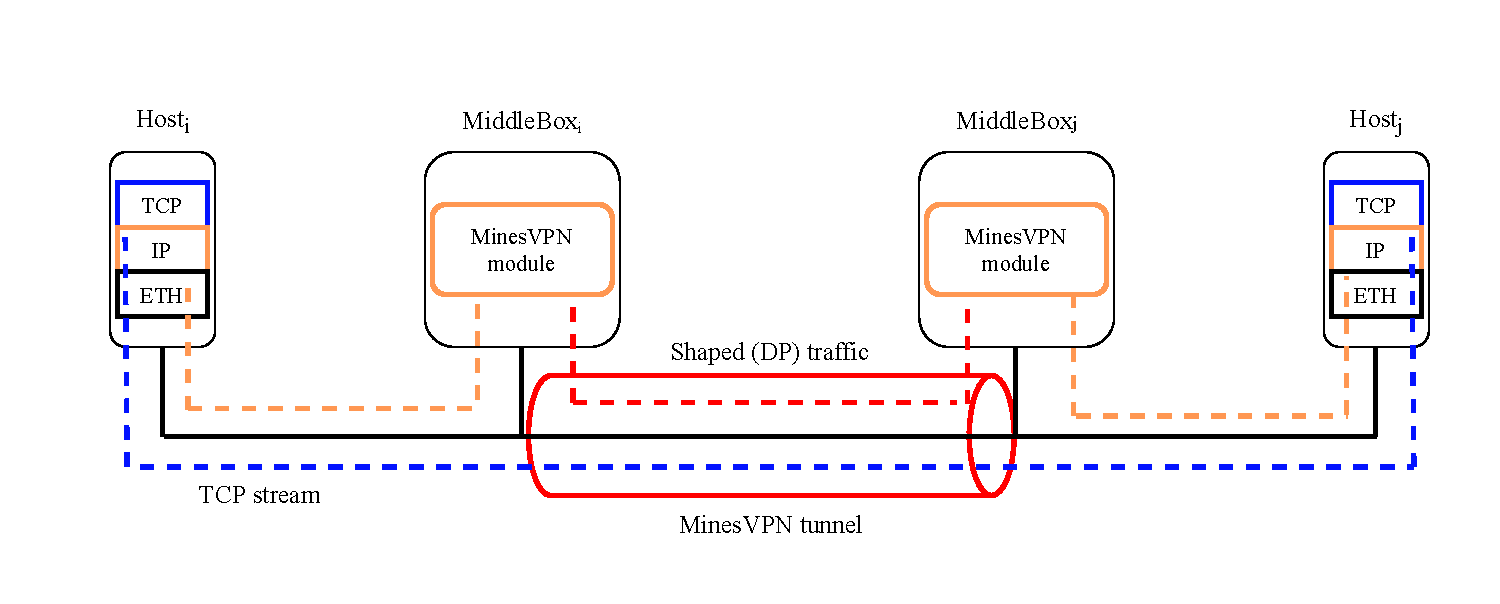
\includegraphics[width=\columnwidth]{figures/Design_highlevel.pdf}
    %  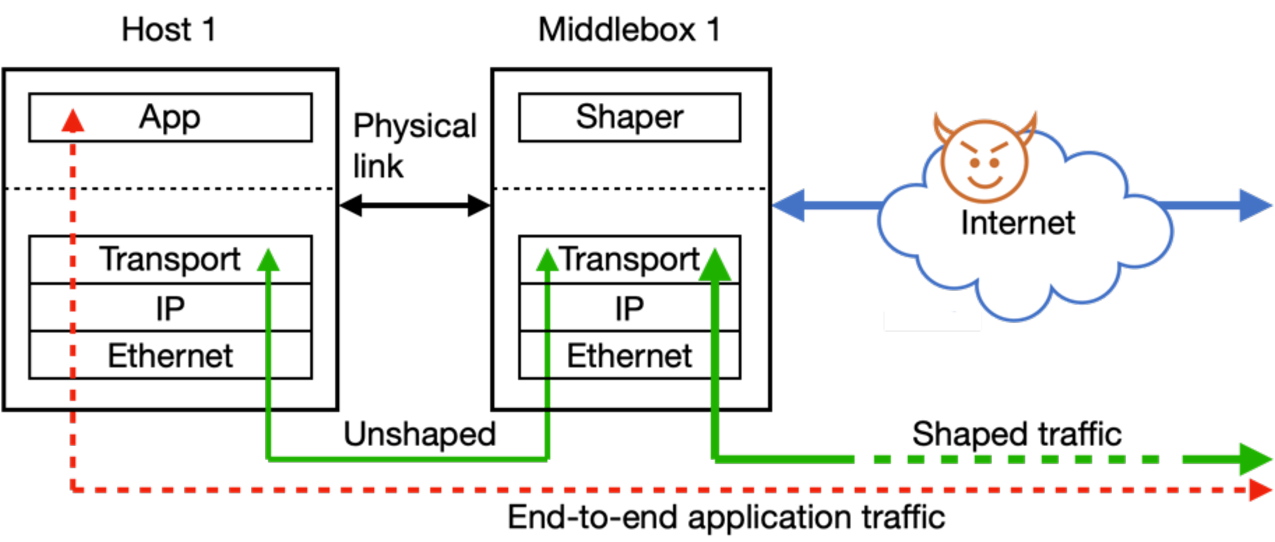
\includegraphics[width=\columnwidth]{figures/minesvpn-overview-half.pdf}
    %  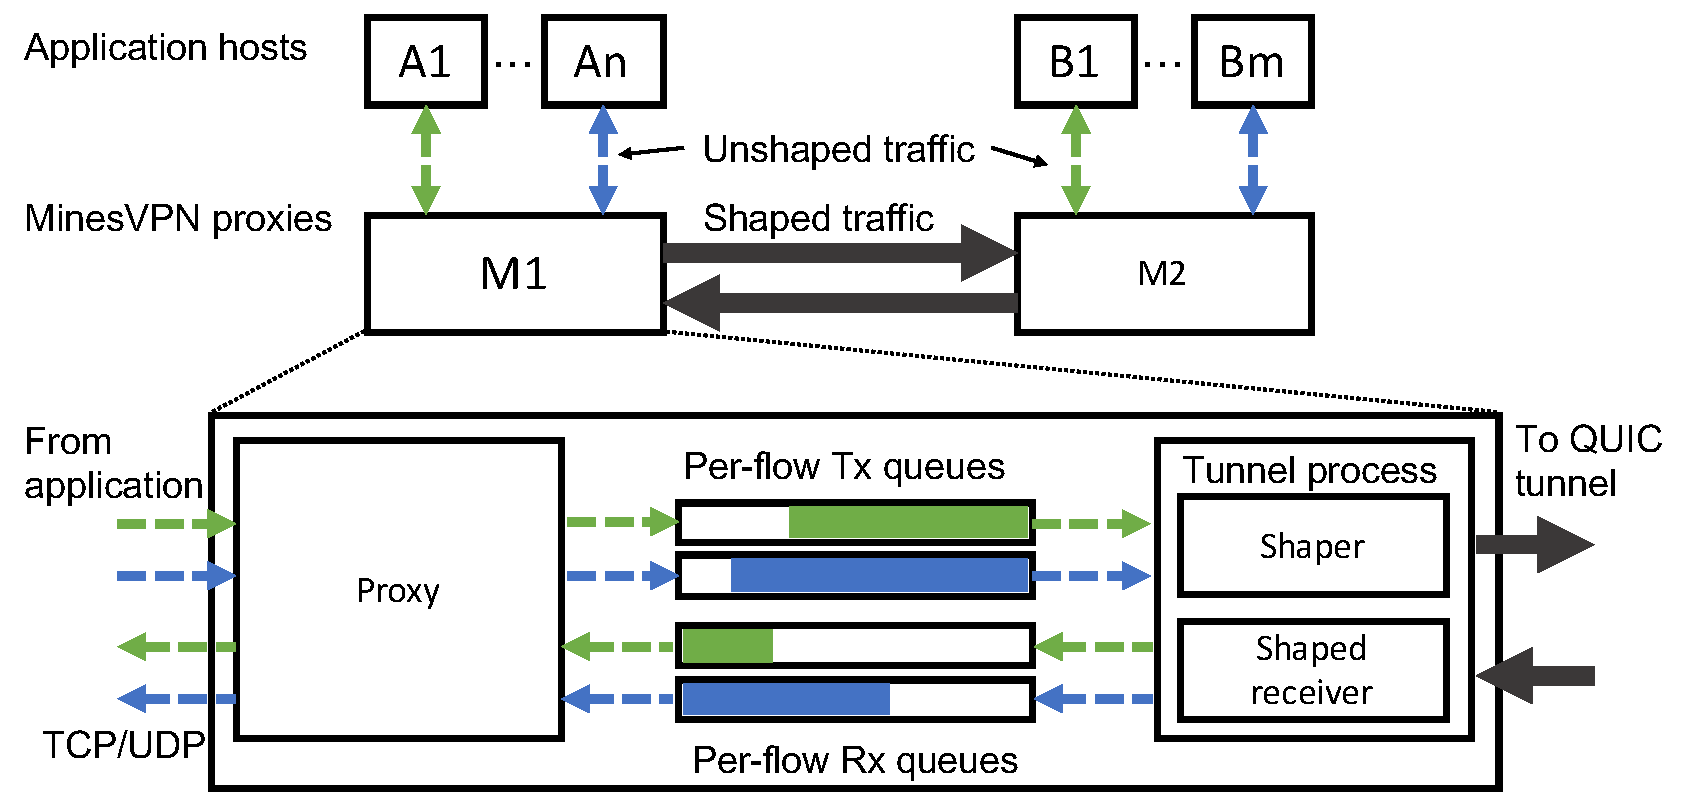
\includegraphics[width=\columnwidth]{figures/minesvpn-arch4.pdf}
    \includegraphics[width=\columnwidth]{figures/design2.pdf}
    \caption{Overview of tunnel design (one endpoint)
        %\am{Update figure}
    }
    \label{fig:minesvpn-overview}
\end{figure}

\subsection{Overview}
\label{subsec:design-overview}

\Cref{fig:minesvpn-overview} shows the design of one endpoint of {\sys}’s
traffic shaping tunnel. A similar endpoint is deployed on the other end of an the tunnel.
%The tunnel endpoints are deployed at both ends of an application’s traffic
%stream.
The endpoints could be integrated with the end hosts or with a gateway at the
edge of an organization’s network. Each tunnel is bidirectional, where the
shape can be configured independently in each direction.

A tunnel endpoint consists of a shaping layer on top of the QUIC protocol,
which in turn runs on top of a standard UDP stack\footnote{In principle, {\sys}
could also rely on a traditional TCP stack.}. The tunnel endpoints establish a
bidirectional QUIC
connection and generate DP-sized transmit buffers in fixed intervals, which
carry payload bytes from one or more application flows.
In the absence of application payload, an endpoint transmits dummy bytes, which are
discarded at the other endpoint.

%An application interacts with the shaping layer through a set of per-flow queues
%carrying the application byte stream. Each flow is mapped to a pair of transmit
%and receive queues.

An application interacts with the shaping layer through a socket connection. For
each application connection, the shaping layer maintains a {\em buffering
queue}, in which it accumulates the application's outbound byte stream before
transforming it into a differentially-private packet sequence.

The security of the tunnel design relies on the key assumption that the traffic
between an application endpoint and the tunnel endpoint is
unobservable to an adversary.
%The security of the tunnel design relies on two key assumptions. First, the
%traffic between an application endpoint and the tunnel endpoint close to it is
%not observable to an adversary, as also mentioned in
%\S\ref{subsec:threat-model}. Secondly, the time required by the shaping layer to
%prepare the DP-sized buffers is independent of application secrets.

\paragraph{Tunnel setup and teardown.}
{When one endpoint of an application initiates communication with
another endpoint, the initiator first establishes a {\sys} tunnel between the
application endpoints before establishing communication with the receiver. The
initiator sends a configuration message to the shaping layer with the source and
destination IP addresses and ports, a reliability flag, and a privacy descriptor.
%\todo{and a tunnel lifetime}.
The reliability flag indicates if the tunnel should provide reliable delivery
semantics or not. The privacy descriptor indicates the DP parameters to be used
for shaping the tunnel traffic.
%\todo{The lifetime indicates the duration for which the tunnel transmits DP
%shaped traffic.}}
%\mis{I don't understand the lifetime: this suggests that someone
%needs to know how long the tunnel needs to exist; doesn't it make more
%sense to have a timeout that says to shut down the tunnel after some
%period of inactivity?}
\mis{About now I keep wanting to say, "No, it's the middlebox" ever time I
see the word endpoint.  I think we need a sentence at the beginning of
Section 4.1 (design overview) that says something like "Although our implementation places tunnel endpoints on a middlebox, for the purposes of our
design, we do not distinguish between the locations of
application endpoints and tunnel endpoints; they could be located on the
same node, or they could be on different nodes as in our implementation.}

Upon receiving a control message, the tunnel endpoint establishes a QUIC
connection with the remote endpoint and configures the reliability semantics
and privacy parameters
%\todo{and tunnel lifetime}
for each direction.
The endpoint also
initializes two QUIC bidirectional streams in the tunnel: control~and
dummy.
The control stream transmits
messages related to the establishment and termination of a connection
between the application endpoints. The dummy stream transmits padding
in QUIC packets in the form of STREAM frames\footnote{We do not use QUIC's
PADDING frames as they do not elicit acknowledgements and hence are
distinguishable from STREAM frames \cite{rfc9000}.}.
%The data streams carry the payload bytes from application flows.

%\todo{After the expiry of the lifetime},
\update{When the tunnel is inactive for a period of time, one of the endpoints
initiates a termination sequence and closes all open QUIC streams and the tunnel
connection.}


\paragraph{Initializing and closing shaped streams.}
%\mis{The sentence that follows desribes setting up a new stream; not
%setting up the tunnel; I think this should be called out separately
%as a step between creating the tunnel and shaping the traffic.}
Once a tunnel is ready, the initiator runs a connection handshake, which is
intercepted in the tunnel.
\todo{The shaping layer establish a new QUIC data stream in
the existing tunnel and maps the new application flow to the new stream.}
The remote tunnel endpoint establishes a connection with the receiver and sets
up the receiver's configurations in the QUIC tunnel.
\todo{When an application flow terminates, the tunnel closes the QUIC data
stream and the connections with the application endpoints.}
The stream setup and closing messages are shaped according to the tunnel's
parameters. \am{Fix the red text.}
%\todo{If a tunnel is already exists between the source and destination IP
%addresses with the same configurations, the shaping layer maps the new
%application flow with one of the unused data streams in the existing tunnel.}
%{\todo{After the expiry of the lifetime}, one of the tunnel endpoints initiates
%a termination sequence and closes all open QUIC streams and the tunnel
%connection.}


\paragraph{Traffic shaping within a tunnel.}
The shaping layer in a tunnel endpoint converts the byte stream of one or more
application flows into a sequence of network packets whose sizes and timing
follow a distribution that guarantees DP.
At periodic intervals, \update{it performs a DP measurement to determine the
number of bytes $\qlendp$ to be~transmitted according to the tunnel's DP
parameters}. It prepares a buffer consisting of $\payload$ payload bytes
and $\dummy$ dummy bytes, where $\payload$ is the minimum of $\qlendp$ and the
application bytes available in the buffering queue, and $\dummy = \qlendp -
\payload$, which may lie between 0 and $\qlendp$. The shaping layer then passes
the buffer along with the position and length of the padding to the QUIC~layer.

QUIC transforms the buffer into one or more STREAM frames based on the
congestion window, the flow window of the receiver endpoint, and the MTU
(maximum transmission unit). It
places the padding bytes into a dummy STREAM frame. QUIC packages the frames
into packets, whose length is at most MTU
minus the length of the headers and whose payload is
encrypted. QUIC forwards the packets to the UDP layer, which subsequently
transmits the prepared packets as quickly as it can, given the line rate of the
NIC.

{\sys} configures the periodic interval such that the shaping layer can prepare
each DP buffer within an interval. If the preparation time for a buffer exceeds
the interval, the shaping layer discards the buffer. This ensures that the
buffering queue length does not grow significantly, which in turn controls the
overhead incurred due to DP shaping.
%\am{Note this is secure only if delays due to cc. All other delays should be
%properly masked.}
%
%We elaborate on the DP model in \S\ref{sec:dp}.
We analyze the impact of the buffering queue~length and the periodic interval
length on privacy guarantees, bandwidth overheads, and latency overheads in
\S\ref{sec:eval}.

\paragraph{Inbound traffic processing within a tunnel.}
A tunnel endpoint receives shaped packets from the tunnel and applies inverse
processing on each packet.
QUIC receives the packet and
sends an ACK to the sender. Subsequently, it decrypts the packet, discards the
dummy frame, extracts the payload bytes from the remaining STREAM frames, and
forwards the payload bytes to the application.

%\paragraph{Configuring privacy requirements.}
%\todo{By default, each flow sent through a single tunnel is subject to the same
%DP parameters. Furthermore, the tunnel aggregates the payload from concurrent
%flows to amortize the padding overheads of DP. However, an application can
%choose to configure the DP parameters separately for each of its flows. Each
%flow with distinct DP parameters requires a separate tunnel.}


%%%\Cref{fig:minesvpn-overview} gives an overview of {\sys}'s design.
%%%Tunnel endpoints (\eg M1 and M2) integrate
%%%shaping within the QUIC protocol, which runs on top of a standard UDP stack.
%%%The
%%%QUIC stack is used by M1 and M2 to communicate with each other and with other
%%%tunnel endpoints, as well as with their local application endpoints A1,
%%%..., An and B1, ..., Bm (respectively)\footnote{In principle, {\sys} could
%%%also
%%%rely on a traditional TCP or a UDP stack based on applications' reliability
%%%requirements.}.
%%%For two application endpoints to communicate, say A1 and B1, a bidirectional
%%%connection is set up between M1 and M2, through which the application traffic
%%%is
%%%shaped and transmitted.
%%%Specifically, M1 terminates the transport connection of A1, and transforms the
%%%byte stream of A1 to B1 into a shaped traffic stream, which is then
%%%transmitted
%%%to M2. Similarly, M2 terminates the transport connection of B1 and shapes the
%%%byte stream from B1 to A1. M1 and M2 shape the traffic in each direction
%%%independently.
%%%
%%%\paragraph{Traffic shaping within a tunnel.}
%%%\todo{A tunnel endpoint converts an application's byte stream into a sequence
%%%of
%%%network packets whose sizes and timing follow a differentially private
%%%distribution.}
%%%%\am{Goes back to my question, can we prove that periodic timing + DP burst
%%%%sizes within periodic intervals $\Rightarrow$ overall DP shape?}
%%%For this, a tunnel endpoint relies on the \todo{primitive} of a {\em buffering
%%%queue}, in which it accumulates the application byte stream before
%%%transforming
%%%it into a differentially-private packet sequence.
%%%
%%%For example, when the tunnel endpoint M1 receives an unshaped byte stream from
%%%its local end host A1, which is destined for end host B1, M1 enqueues the byte
%%%stream into the buffering queue. After every periodic time interval $T$, M1
%%%computes the number of bytes $n$ to be transmitted in the next interval
%%%according to the DP parameters of the corresponding tunnel between M1 and M2.
%%%M1
%%%prepares a buffer with a number of bytes $r$ that is the minimum of the number
%%%of the number of application bytes available in the buffering queue and $n$,
%%%and
%%%generates additional $d = n - r$ dummy bytes if required. M1 then adds a
%%%padding
%%%header to the buffer to indicate the position and length of the padding,
%%%and encrypts the buffer and the padding header. Finally, M1 transforms the
%%%buffer into one or more network packets of at most MTU length (maximum
%%%transmission unit) and transmits the prepared packets as fast as it
%%%can given the line rate of the connected NIC and the congestion conditions of
%%%the downstream network.
%%%
%%%The size of the buffering queue and the length of the periodic intervals
%%%determine the tradeoffs between privacy guarantees, bandwidth overheads, and
%%%latency overheads of {\sys}. We elaborate on the DP model in \S\ref{sec:dp}
%%%and
%%%evaluate the tradeoffs in \S\ref{sec:eval}.
%%%\am{explicitly mention dropping of queue data if not consumed within fixed
%%%interval.}
%%%
%%%\if 0
%%%When a tunnel endpoint M1 receives an unshaped byte stream from its local end
%%%host A1, which is destined for end host B1, M1 transforms the byte stream
%%%into
%%%a
%%%sequence of buffers whose sizes follow a noise distribution defined by the DP
%%%parameters of the corresponding tunnel between M1 and M2, and which are then
%%%transmitted at periodic intervals.
%%%Specifically, after every periodic time interval $T$, M1 computes the number
%%%of
%%%bytes $n$ to be transmitted in the next interval according to DP. M1 prepares
%%%a
%%%buffer with a number of bytes $r$ that is the minimum of the number of bytes
%%%available in the application's byte stream and $n$ and generates additional
%%%$d$
%%%= $n - r$ dummy bytes if required. M1 then adds a padding header to the
%%%buffer
%%%to
%%%indicate the position and length of the padding, encrypts the buffer and the
%%%padding header, adds the protocol headers of the tunnel's network stack, and
%%%transmits the prepared packets as fast as it can given the line rate of the
%%%connected NIC and the congestion conditions on the downstream network.
%%%\fi
%%%
%%%
%%%\paragraph{Inbound traffic processing within a tunnel.}
%%%Each tunnel endpoint receives shaped packets from the tunnel and process them
%%%in
%%%the reverse order. For instance, when the tunnel endpoint M1 receives packets
%%%from M2, which are sent from end host B1 to A1, M1 strips the tunnel protocol
%%%headers, decrypts the buffer, discards the dummy bytes, and forwards the
%%%payload
%%%bytes to A1.

%%The packets are
%%processed in the endpoint in the reverse order: the tunnel protocol headers are
%%stripped, the content is decrypted and payload bytes are forwarded to the end
%%host, while dummy bytes are discarded at the endpoint.

\if 0
\subsection{Security Guarantees \am{to be revised}}
\label{susbec:design-security}
%{\sys}'s design satisfies the security requirements as follows.

\am{We should show design follows the DP spec and implementation follows the
design. Therefore, we have a secure solution by design and construction.}
\am{Combine security analysis of design and implementation and move to
evaluation?}
{\sys}’s design provides the following security property: an adversary cannot
infer application secrets \todo{or the number of active participants} by
observing the tunnel traffic. This property holds because:
%
%{\bf S1.} The traffic between an application endpoint and the tunnel endpoint
%close to it is not observable to an adversary (by assumption).
%
{\bf S1.} All payload traffic of a sensitive flow passes through a tunnel and is
subjected to shaping and encryption.
%
{\bf S2.} The shaping layer prepares differentially-private sized buffers and
passes the buffers to QUIC in fixed intervals. Subsequently, the QUIC layer may
transmit the buffers in one or more packets. However, by the post processing
argument of DP \citeme{dp-postprocessing}, the shape of the packets still
provides DP. (The proof of DP is in \todo{\S\ref{appendix:dp}}.)
%
%\todo{{\bf S2.} The tunnel continuously transmits DP shaped traffic, which
%hides the start and end times of application transmissions.}
%
\todo{{\bf S3.} The privacy guarantees of a tunnel are configured before the
start of application transmission and do not change during the tunnel lifetime.}
\todo{{\bf S4.} The time required by the shaping layer to
prepare the DP-sized buffers is independent of application secrets. This is
because {\sys}'s periodic interval is configured such that it can handle all DP
sizes. Thus, any delays in transmitting the buffers can only arise due to
congestion or packet losses in the tunnel network, which are secret-independent
events.}
\fi

%\todo{Note: If we want this to be completely transparent, we might have to do
%some IP Spoofing and will have to include that in our mechanism}

%\subsection{Shaping Module}
%This module has the following responsibilities as a sender:
%\begin{itemize}
%    \item Determine the number of bytes (n) to send in the next time slot
%    \item Obtain 'n' bytes from the Non-DP Queue
%    \item Add dummy bytes if necessary (if Non-DP Queue size < n)
%    \item Add the DP Header populated with all the necessary information
%    \item Encrypt the payload (n bytes of data + DP header)
%    \item Send it out to the other middle-box
%\end{itemize}
%
%It also acts as a receiver and performs the following tasks:
%\begin{itemize}
%    \item Decrypt the payload
%    \item Obtain the DP header to determine padding, actual destination etc
%    \item Extract the actual payload and send it to the Middle-box Module
%\end{itemize}

%\begin{table}[t]
%    \centering
%    \renewcommand{\arraystretch}{1.2}
%    \begin{tabular}{lll}
    %        \toprule
    %        {\bf Outer/Inner} & {\bf TCP} & {\bf UDP}
    %        \\
    %        \midrule
    %        {\bf TCP} & meltdown & inefficient
    %        \\
    %        {\bf UDP} & insecure & inefficient
    %        \\
    %        \bottomrule
    %    \end{tabular}
%    \caption{Impact of tunneling a transport inside transport}
%    \label{tab:transport-in-transport}
%\end{table}



\section{Traffic Shaping Tunnel}
\label{sec:design}

%\todo{Design goals look rather similar to Pacer.}
%The previous section describes an abstract differentially private traffic
%shaping strategy.
%We now present \sys's traffic-shaping tunnel.
%
A tunnel must address three requirements.
First, it must satisfy DP guarantees. For this, the tunnel~must complete DP
queries and prepare shaped packets within each interval, and it
must be able to transmit all payload bytes generated from an application within
a finite window length (as defined in the DP strategy).
%
Secondly, the payload and dummy bytes in the shaped packets must be
indistinguishable to an adversary. For this, the payload and dummy bytes must be
transmitted through a shared transport layer so that they are identically
acknowledged by the receiver and subject to congestion control and
loss recovery mechanisms.
%
Finally, the tunnel must provide similar levels of reliability,
congestion control, and loss recovery as expected by the application.

\if 0
A traffic shaping tunnel must address three requirements.
%{\bf R1.} It must ensure that the payload is unobservable to an adversary from
%the traffic shape. The packet sizes and timing may be correlated with
%application secrets or the application's sending or receiving rate (\ie flow
%control), which in turn may be secret-dependent.
{\bf R1.} Given a sequence of packets whose sizes and timing reveal the payload,
the tunnel must produce a packet sequence whose sizes and timing do not reveal
information about the payload.
{\bf R2.} It must protect against an adversary observing packets
along the entire path between the tunnel endpoints.
{\bf R3.} It must provide similar levels of reliability, congestion control, and
loss recovery as the original packet sequence.

R1 requires that the tunnel implements DP shaping correctly. Specifically,
it must complete DP decision making and preparation of a shaped buffer within
each interval (as defined in the DP shaping strategy). Moreover, it must be able
to transmit all payload bytes generated from an application within a finite
window length (defined in the DP shaping strategy).
R2 and R3 require that a tunnel implements padding in the outbound packets above
the transport layer so that it is delivered and acknowledged by the destination
and retransmitted upon loss in the same way as application payload.
%R2 requires that a tunnel must ensure that both payload and padding is delivered
%and elicit acknowledgements from the destination and, thus, must apply padding
%in the outbound packets before the transport layer packets are constructed.

One way to address all the requirements is to tunnel the transport layer
protocol between the application endpoints through {\sys}'s tunnel.
However, tunneling UDP through any protocol can be inefficient,
and tunneling
TCP through TCP can cause a TCP meltdown \cite{honda2005tcpovertcp,
tcp-meltdown}.
Tunneling TCP through UDP is insecure: TCP between the application end hosts
handles retransmission of lost payload bytes only,
not of any dummy bytes injected between the tunnel endpoints, making padding
observable.
\fi

%R1 requires that the tunnel must complete DP measurements and prepare shaped
%buffer within each decision interval, and it must be able to transmit all
%payload bytes generated from an application within a finite window length (as
%defined in the DP shaping strategy).
%R3 requires that the tunnel implements a transport protocol that subjects
%application's traffic to similar mechanisms as expected by the the application,
%and
%R2 requires that the dummy bytes are transmitted above the transport layer so
%that they are acknowledged by the destination and subject to the identical
%congestion control and loss recovery mechanisms as the payload bytes.

\Cref{fig:minesvpn-overview} shows the design of one endpoint of {\sys}’s
traffic shaping tunnel. A similar endpoint is deployed on the other end of
the tunnel.
%\ml{and bi-directional streams' privacy loss is the DP composition
%of the privacy loss in each direction}.
%The endpoints could be integrated with the end hosts or with a gateway at the
%edge of an organization’s network. Each tunnel is bidirectional, where the
%shape can be configured independently in each direction.
%
{The shape of the traffic in the tunnel can be configured independently
in each direction. The privacy loss in bidirectional streams is the DP
composition of the privacy loss in each direction.}

A tunnel endpoint consists of a shaping layer (Shaper) on top of QUIC, which
in turn runs on top of a standard UDP stack.
%\footnote{Instead of QUIC/UDP, {\sys} could also use a traditional TCP stack.}.
The tunnel endpoints establish a
bidirectional QUIC connection and generate DP-sized transmit buffers in fixed
intervals, which carry payload bytes from one or more application flows. In the
absence of application payload, a tunnel endpoint transmits dummy bytes, which
are discarded at the other endpoint. QUIC encrypts all outbound packets.
%Each tunnel is bidirectional, where the shape can be configured independently in
%each direction.

%An application interacts with the shaping layer through a set of per-flow queues
%carrying the application byte stream. Each flow is mapped to a pair of transmit
%and receive queues.

{\sys} adopts a transport-layer proxy architecture: each application
terminates a connection with its local tunnel endpoint. The application byte
stream is sent to the remote application over three piecewise connections: (i)
between the application and its local tunnel endpoint, (ii) between the
tunnel endpoints, and (iii) between the remote tunnel endpoint and the remote
application.
This ensures only one active congestion control and reliable delivery mechanism
in the tunnel and that all bytes are subject to identical mechanisms\footnote{
We discard tunneling TCP through TCP as it causes TCP
meltdown~\cite{honda2005tcpovertcp, tcp-meltdown}, or TCP through UDP as it is
unsafe.
(TCP between the application hosts would retransmit lost payload bytes
only, not any dummy bytes injected between the tunnel endpoints, making the
dummy bytes observable.)
%Tunneling TCP within TCP can cause a TCP meltdown \cite{honda2005tcpovertcp,
%tcp-meltdown}. Tunneling TCP through UDP is insecure: TCP between the
%application hosts would handle retransmission of lost payload bytes only, not of
%any dummy bytes injected between the tunnel endpoints, making the dummy bytes
%observable.
}.
%Moreover, payload and dummy bytes are subject to identical mechanisms in the
%tunnel, ensuring that they are indistinguishable to an adversary along the
%entire tunnel path.
%This architecture satisfies both the security and practical requirements of a
%traffic shaping tunnel.
%For ease of implementation, our prototype requires applications to explicitly
%connect to a tunnel endpoint.
%In principle, {\sys} can also transparently proxy application
%connections.

%An application interacts with the shaping layer through a socket connection. For
%each application connection, the shaping layer maintains a {\em buffering
%queue}, in which it accumulates the application's outbound byte stream before
%transforming it into a differentially-private packet sequence.

The application and the tunnel endpoint shown in \Cref{fig:minesvpn-overview}
could either be colocated on the same host or located on separate hosts.
%For example, the tunnel endpoint could be on a separate middlebox or integrated
%with a gateway at the edge of an organization's network.
In each case, the traffic between the application and the tunnel endpoint is
assumed to be unobservable to an adversary.
Our design (\S\ref{subsec:design-overview}) does not distinguish between the two
configurations.
Our implementation (\S\ref{sec:implementation}) assumes that the tunnel endpoint
is located on a separate middlebox. We discuss security in
\S\ref{subsec:impl-security} and alternate deployments in
\S\ref{subsec:design-discussion}.

\if 0
The tunnel endpoints could be integrated with the application hosts or with a
gateway at the edge of an organization’s network.
\todo{Although our implementation places tunnel endpoints on a middlebox, for
the purposes of our design, we do not distinguish between the locations of
application endpoints and tunnel endpoints; they could be located on the
same node, or they could be on different nodes as in our implementation.}
%Each tunnel is bidirectional, where the shape can be configured independently
%in each direction.
The security of the tunnel design relies on the key assumption that the traffic
between an application endpoint and the tunnel endpoint is unobservable to an
adversary.
%The security of the tunnel design relies on two key assumptions. First, the
%traffic between an application endpoint and the tunnel endpoint close to it is
%not observable to an adversary, as also mentioned in
%\S\ref{subsec:threat-model}. Secondly, the time required by the shaping layer to
%prepare the DP-sized buffers is independent of application secrets.
\fi

\subsection{Tunnel Design and Operations}
\label{subsec:design-overview}

\textbf{Tunnel setup and teardown.}
%When one endpoint of an application initiates communication with
%another endpoint, the initiator first establishes a {\sys} tunnel between the
%application endpoints before establishing communication with the receiver.
%Before establishing communication with a receiver, an initiator application
%first establishes a {\sys} tunnel between the application endpoints.
\update{Before applications can communicate with each other, a {\sys} tunnel
must be set up between their local tunnel endpoints.
The initiator application sends a configuration message to its local tunnel
endpoint with the source and destination IP addresses and ports, a reliability
flag, and a privacy descriptor.}
%\todo{and a tunnel lifetime}.
The reliability flag indicates if the tunnel should provide reliable delivery
semantics or not. The privacy descriptor indicates the DP parameters to be used
for shaping the tunnel traffic.
%\todo{The lifetime indicates the duration for which the tunnel transmits DP
%shaped traffic.}
%\mis{I don't understand the lifetime: this suggests that someone
%needs to know how long the tunnel needs to exist; doesn't it make more
%sense to have a timeout that says to shut down the tunnel after some
%period of inactivity?}
%\mis{About now I keep wanting to say, "No, it's the middlebox" ever time I
%see the word endpoint.  I think we need a sentence at the beginning of
%Section 4.1 (design overview) that says something like "Although our
%implementation places tunnel endpoints on a middlebox, for the purposes of our
%design, we do not distinguish between the locations of
%application endpoints and tunnel endpoints; they could be located on the
%same node, or they could be on different nodes as in our implementation.}

Upon receiving a configuration message, the Shaper establishes a QUIC
connection with the remote tunnel endpoint and configures the reliability
semantics and privacy parameters
%\todo{and tunnel lifetime}
for each direction.
It also initializes \todo{three types of bidirectional~streams in the tunnel:
control, dummy, and data streams}.
One {\em control stream} is used to transmit
messages related to the establishment and termination of a connection
between the application endpoints. A {\em dummy stream} transmits padding
in QUIC packets in the form of STREAM frames\footnote{We do not use QUIC's
PADDING frames as they do not elicit acknowledgements and hence are
distinguishable from STREAM frames \cite{rfc9000}.}.
%\ml{random pref: I would not make that a footnote.}
\todo{The tunnel pre-configures a finite number of data streams, which carry
payload bytes from one or more application flows.}

%\todo{After the expiry of the lifetime},
{When the tunnel is inactive for a period of time, one of the tunnel
endpoints initiates a termination sequence and closes all open QUIC streams and
the tunnel connection.}
%\ml{why? Doesn't that leak no user in the recent past? maybe it's ok?}


\textbf{Connection establishment and termination.}
Once a tunnel is ready, applications can establish and terminate connections
with each other, which is mediated by the tunnel.
When the initiator application runs a connection establishment handshake with
its local tunnel endpoint, the Shaper maps the application flow to
a per-flow buffering queue and one of the inactive QUIC data streams in the
tunnel, and notifies the remote tunnel endpoint.
The remote tunnel endpoint establishes a connection with the receiver
application and maps the receiver application's flow with the data stream.
The connection termination handshake is handled similarly by the tunnel
endpoints. The messages for connection establishment and termination are
transmitted over the control stream in the tunnel and shaped according to the
tunnel's parameters.
%Once a tunnel is ready, the initiator application runs a connection handshake,
%which is intercepted in the local tunnel endpoint.
%\todo{The Shaper maps the application flow to one of the inactive data streams
%in the tunnel.}
%%\todo{The Shaper establishes a new QUIC data stream in
%%the existing tunnel and maps the new application flow to the new stream.}
%The remote tunnel endpoint establishes a connection with the receiver and sets
%up the receiver's configurations in the QUIC tunnel.
%%\todo{When an application flow terminates, the tunnel closes the QUIC data
%%stream and the connections with the application endpoints.}
%\todo{When an application flow terminates, the tunnel unmaps the QUIC data
%stream and closes the connections with the applications.}
%\todo{The connection termination messages for applications}
%The stream setup and closing messages are shaped according to the tunnel's
%parameters. \am{Fix the red text.}
%\todo{If a tunnel is already exists between the source and destination IP
%addresses with the same configurations, the shaping layer maps the new
%application flow with one of the unused data streams in the existing tunnel.}
%{\todo{After the expiry of the lifetime}, one of the tunnel endpoints initiates
%a termination sequence and closes all open QUIC streams and the tunnel
%connection.}


\textbf{Outbound traffic shaping.}
%For each application flow, the Shaper maintains a {\em buffering
%queue}, in which it accumulates the application's outbound byte stream before
%transforming it into a differentially-private packet sequence.
The Shaper accumulates the outbound bytes of an application flow in a
buffering queue before it transmits them in packets whose sizes and timing
follow a distribution that guarantees DP.
Within a tunnel, the Shaper transmits bytes from all active flows into a
differentially-private packet sequence.
%The Shaper in a tunnel endpoint converts the byte stream of one or more
%application flows into a sequence of network packets whose sizes and timing
%follow a distribution that guarantees DP.
At periodic intervals, {called DP shaping intervals,} it performs a
DP query on the per-flow queues to determine the
number of bytes $\qlendp$ to be~transmitted according to the tunnel's DP
parameters. It prepares a {\em shaped buffer} consisting of $\payload$ payload
bytes and $\dummy$ dummy bytes, where $\payload$ is the minimum of $\qlendp$ and
the application bytes available in the buffering~queues, and $\dummy = \qlendp -
\payload$, which may lie between 0 and $\qlendp$. The Shaper then passes
the buffer with the position and length of the padding to QUIC.

QUIC transforms the shaped buffer into one or more STREAM frames based on the
congestion window, the flow window of the receiver endpoint, and the MTU
(maximum transmission unit). It
places the padding bytes into a dummy STREAM frame. QUIC packages the frames
into packets, whose length is at most MTU
minus the length of the headers and whose payload is
encrypted. QUIC forwards the packets to the UDP layer, which subsequently
transmits the prepared packets as quickly as it can, given the line rate of the
NIC.

To enforce \Cref{assumption:window}, the Shaper tracks the expiry time of
each byte enqueued in $\buffQ$ based on the arrival time and the neighboring
window length $\winlen$ configuration. The Shaper drops the untransmitted bytes
in the queue upon their expiry.

%\todo{{\sys} configures the {DP shaping} interval such that the Shaper can
%prepare each shaped buffer within the interval. If the preparation time for a
%buffer exceeds the interval, the Shaper discards the buffer. This ensures that
%the buffering queue length does not grow significantly, which in turn controls
%the overhead incurred due to DP shaping.}
%\am{Note this is secure only if delays due to cc. All other delays should be
    %properly masked.}
%

%%%%%%%%%%%%%%%%%%%%%%%%%%%%%%%%%
%% mentioned at the end of sec 3.
%%%%%%%%%%%%%%%%%%%%%%%%%%%%%%%%%
%We evaluate the impact of the buffering queue length and the DP
%shaping interval on privacy guarantees, bandwidth overheads, and latency
%overheads in \S\ref{sec:eval}.

\textbf{Inbound traffic processing.}
A tunnel endpoint receives shaped packets from the tunnel and applies inverse
processing on each packet.
QUIC receives the packet and
sends an ACK to the sender. Subsequently, it decrypts the packet, discards the
dummy frame, and forwards the payload bytes from the remaining STREAM frames to
the application.
%\as{Comment 7: we should add a paragraph here, explaining that the tunnel
%endpoint is modular. It does not necessarily require to be in a middlebox. We
%chose it to be in a middlebox for reasons we provide in next section.}

\subsection{Middlebox Implementation}
\label{sec:implementation}

\begin{figure}[t]
    \centering
    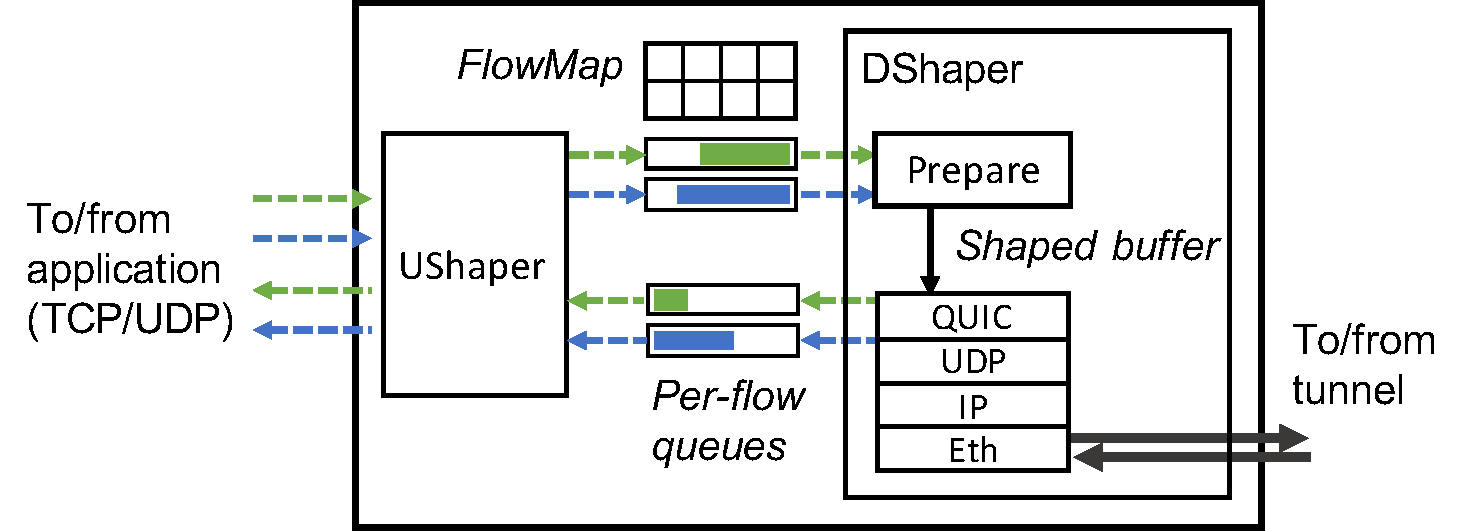
\includegraphics[width=\columnwidth]{middlebox-arch3.pdf}
    %    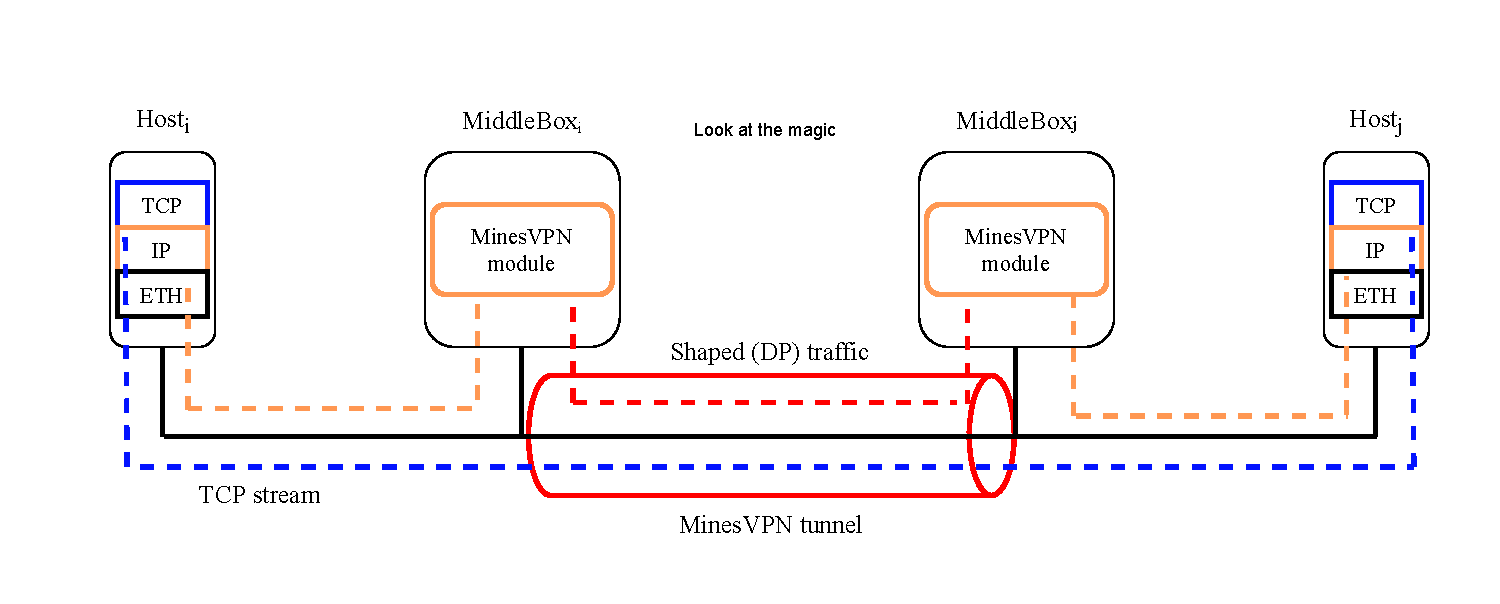
\includegraphics[width=\columnwidth]{figures/design.pdf}
    \caption{{\sys} middlebox design}
    \vspace{-0.4cm}
    \label{fig:minesvpn-impl}
\end{figure}

We present a middlebox-based {\sys} implementation.
%as shown in \Cref{fig:minesvpn-impl}.
%
%Recall from \S\ref{subsec:key-ideas}, a middlebox can support shaping for
%several applications and amortizes~the shaping cost among multiple flows that
%share the same tunnel.
%%Moreover, middleboxes can support ``long-term'' tunnels between
%%endpoints. Such tunnels may be set up, for instance, between organization
%%campuses to secure all communication between the campuses without the need for
%%modifying individual application hosts.
%
For ease of implementation, our prototype requires applications to explicitly
connect to the middleboxes.
In principle, {\sys} can transparently proxy application
connections.

%Following the proxy architecture, the middlebox splits the communication between
%two application endpoints over three transport connections:
%one between two middlebox endpoints that provides a tunnel and one between
%each application endpoint and its local middlebox.
In our implementation (see \Cref{fig:minesvpn-impl}), a middlebox consists of
two userspace processes. The
{\ushaper} mediates {\em unshaped} traffic between the applications and the
middleboxes. The {\dshaper} handles {\em DP shaped} traffic within the tunnel.

%\subsection{Components}
%\label{subsec:impl-mediation}
\textbf{UShaper.}
%The {\ushaper} mediates the unshaped traffic between one or more local
%application endpoints and the {\dshaper} using per-flow transmit and receive
%queues.
%It implements
The {\ushaper} implements a transport server (or client) for interfacing with
each local client (or server, respectively) application.
%\footnote{The {\ushaper} could also be a SOCKS5 proxy \cite{torpt}.}.
%\ml{random pref: wouldn't use a footnote here}
%The type of the transport endpoint depends on the application's choice of
%transport protocol.
For managing multiple flows, it shares a {\flowmap} table with the {\dshaper},
which consists of an entry for each end-to-end flow. Each entry maps the
piecewise connections with
%the associated sockets of {\ushaper} and {\dshaper}, a
a pair of transmit and receive queues to carry the local application's byte
stream, and shaping configurations (\eg privacy descriptor) provided by an
%\todo{(\eg privacy descriptor, tunnel lifetime)} provided by an
application at the time of flow registration.
%The transmit queues of the end-to-end flows mapped to a single tunnel connection
%correspond to the tunnel's buffering queue, on which tunnel's DP guarantees
%rely.

The {\ushaper} receives the outbound traffic from a sender application
and enqueues the byte stream into a per-flow transmit queue shared with the
{\dshaper}.
It also dequeues bytes from a per-flow receive queue, repackages them
into transport packets and sends them to the receiver application.

%\if 0
\begin{figure}[t]
    \centering
    %    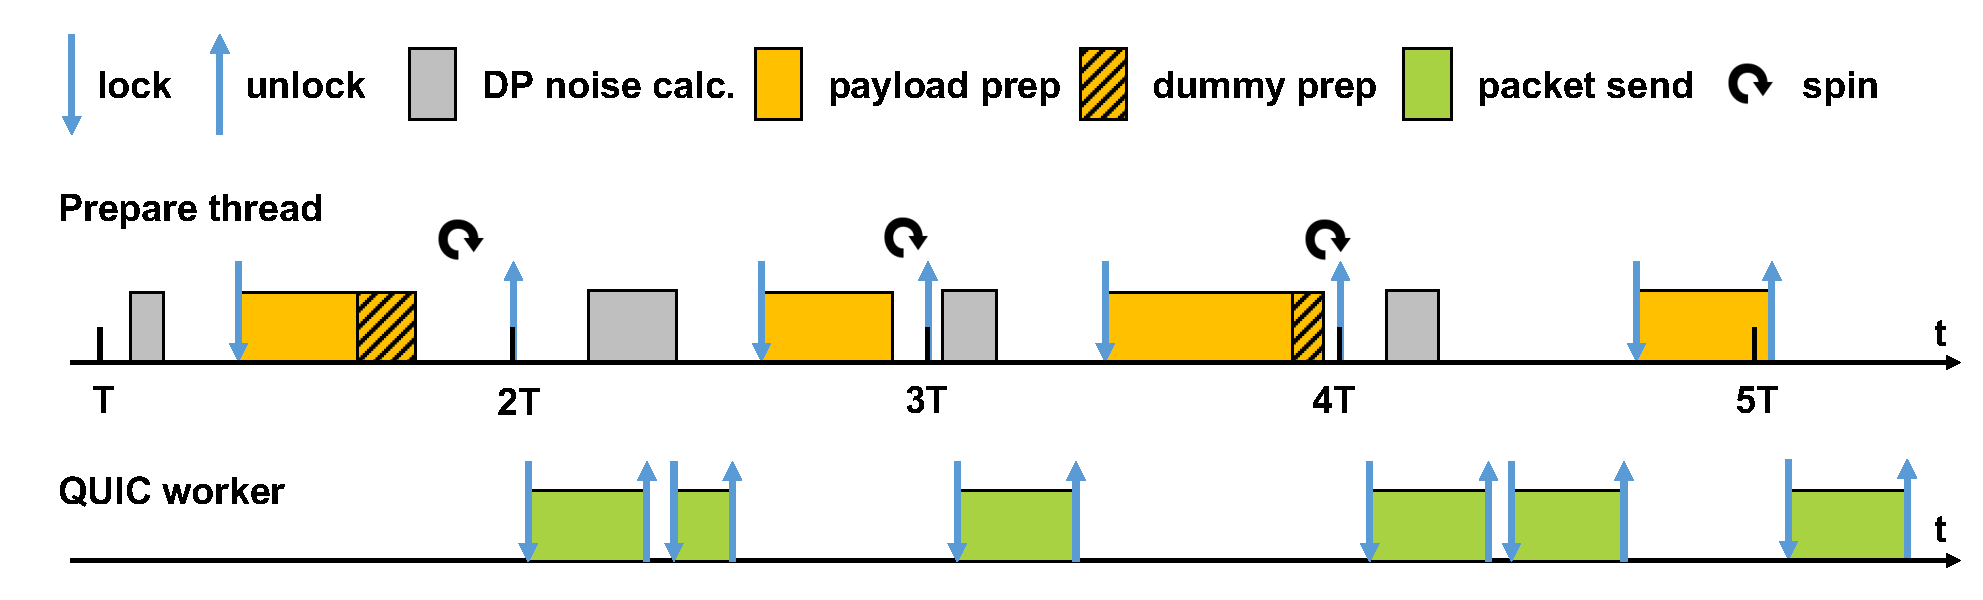
\includegraphics[width=\columnwidth]{figures/schedule.pdf}
    \includegraphics[width=\columnwidth]{schedule5.pdf}
    \caption{{\dshaper} schedule}
    \vspace{-0.4cm}
    \label{fig:middlebox-schedule}
\end{figure}
%\fi

\textbf{DShaper.}
%
The {\dshaper} consists of a {\prepare} thread and a QUIC
worker thread.
The {\prepare} thread instantiates a QUIC client/server to establish
a tunnel with the remote middlebox and implements the DP shaping logic.
%On~the transmit side, {\prepare} examines the number of bytes in each
%per-flow transmit queue, determines the number of bytes to transmit,
On the transmit side, {\prepare} {prepares shaped buffers based on DP
queries on the transmit queues}
and then submits shaped buffers to the QUIC worker for transmission.
On the receive size, the QUIC worker transmits ACK frames to the sender
and then decrypts the QUIC packets, extracts the STREAM frames, and copies
bytes (including dummy bytes) from each frame into the appropriate per-flow
receive queue.

%\noindent
\textbf{Ensuring secret-independent shaping.}
%\as{Comment 1.1: We should rewrite this section from scratch, showing that all
%we perform is a best-effort guarantee.}
%\label{subsec:impl-shaping-security}
%\Cref{fig:middlebox-schedule} illustrates the schedule of operations on
%{\prepare}
%and QUIC worker threads on the outbound path.
%The green and orange boxes represent data-independent and data-dependent
%operations, respectively.
%\todo{
%To enforce DP guarantees, intuitively, the middlebox must ensure that {\em
%an adversary observes $\qlendp$ bytes in each transmit interval $\dpintvl$.}
To enforce DP guarantees, {\dshaper} should {\em transmit} exactly $\qlendp$
bytes in each DP shaping interval $\dpintvl$.
%\ml{not really right? It's that it observes a number of bytes---and any
%observable quantity---that is a post-processing of the DP measurements. Hence,
%any observable quantity cannot depend on application data other than throught
%the DP measurements.}
%}
%
\if 0
Let us first understand the factors that might prevent the middlebox from
guaranteeing this property.
Even though an application is physically isolated from the middlebox and can
encrypt its data (\eg using end-to-end TLS), its flow control behavior could be
secret-dependent and could affect the middlebox's execution.
For instance, the presence or absence of payload traffic from an application
can affect the time {\dshaper} requires to prepare the shaped buffers.
\fi
%
%Ensuring the high-level goal mentioned above requires that
This would require ensuring:
{\bf P1.} {\prepare} computes $\qlendp$, allocates and prepares a buffer
of length
$\qlendp$, and passes the buffer to the QUIC worker within $\dpintvl$,
{\bf P2.} the QUIC worker prepares encrypted packets from the buffer and sends
them to UDP, such that the total payload size of the QUIC packets prepared in
$\dpintvl$ is $\qlendp$, and
{\bf P3.} the~UDP stack transmits packets totaling to $\qlendp$ payload bytes
to the NIC in $\dpintvl$.
Enforcing all these properties would require a constant-time implementation for
each step, which is non-trivial, or a strict time-triggered schedule
for each step, which would significantly reduce link utilization and increase
packet latencies.
%transmission latencies.
%Moreover, the value of $\dpintvl$ required would be large to account for
%potential secret-dependent (\eg flow control) as well as secret-independent
%delays (\eg congestion control).
%This would significantly increase packet transmission latencies.

%\todo{Thanks to DP post processing, however, it suffices to ensure that the
%middlebox {\em prepares} a shaped buffer based on a DP measurement $\qlendp$
%within each time interval $\dpintvl$, \ie property P1. As long as the shaped
%buffers are transformed into network packets independently of the DP
%measurement, the sizes and timing of network packets need not be constrained in
%any way.
%}
\todo{Thanks to DP post processing, however, it suffices to ensure the property
P1,
%\ie that {\dshaper} {\em prepares} a shaped buffer based on a DP measurement
%$\qlendp$ within each time interval $\dpintvl$,
and {\bf P4.} that the QUIC worker transforms the shaped buffer into network
packets independently of the
%\ml{\sout{DP measurement in {\dshaper}}
application data.
%}.
%\ml{\sout{With this, the sizes and timing of network packets need not be
%constrained in any way.}
No other constraint on the sizes and timing of network packets is required to preserve DP.
%}
}

Satisfying P1 involves one challenge. Although the application is physically
isolated from the middlebox, its flow control behavior could be
secret-dependent and could affect the middlebox's execution.
For instance, the presence or absence of payload traffic from an application
can affect the time {\dshaper} requires to prepare the shaped buffers.

%{\dshaper} instead provides the following guarantees. \ml{this makes it sounds
%like we provide weaker than ideally needed guarantees. But we don't! We provide
%what we need to make the observable quantities be a data independent
%post-processing of DP measurements. If the above framing I suggested sounds
%good, this statement probably needs to not be an instead.}
Thus, {\dshaper} satisfies P1 as follows (see \Cref{fig:middlebox-schedule} for
reference).
%The {\dshaper} provides two guarantees.
First, {\prepare} {guarantees that $\qlendp$ is computed with a DP query
in each interval}.
Secondly, {\prepare} guarantees that a shaped buffer of length $\qlendp$ is {\em
prepared} within a fixed time $\dpintvl_{prep}$ within each interval.
Thirdly, {\prepare} locks the shaped buffer for a fixed time,
$\dpintvl_{enq}$, during which it enqueues the buffer for a QUIC
worker.
This ensures that~the buffer is completely enqueued before QUIC starts
transmitting it and that QUIC receives the buffer only at fixed delays.

%\todo{
We empirically profile the time taken by {\prepare} for preparing and enqueueing
shaped buffers for various DP lengths. We set $\dpintvl_{prep}$ and
$\dpintvl_{enq}$ to maximum values determined from profiling, and $\dpintvl$ to
the sum of these maximum values, \ie $\dpintvl_{max}$.
If {\prepare} takes time less than
$\dpintvl_{prep}$ (or $\dpintvl_{enq}$, respectively) to prepare (or enqueue) a
shaped buffer, it sleeps until the end of the interval before moving to the next
phase.
%}
%\todo{We empirically profile the maximal time $\dpintvl^{max}_{prep}$ and
%$\dpintvl^{max}_{enq}$ taken by {\prepare} for preparing and enqueueing shaped
%buffers for various DP sizes. We set $\dpintvl_{prep} = \dpintvl^{max}_{prep}$,
%$\dpintvl_{enq} = \dpintvl^{max}_{enq}$, and $\dpintvl = \dpintvl^{max}_{prep} +
%\dpintvl^{max}_{enq}$. If {\prepare} takes time less than
%$\dpintvl^{max}_{prep}$ (or $\dpintvl^{max}_{enq}$, respectively),
%to prepare (or enqueue) a shaped buffer,
%it sleeps until the end of the interval before moving to the next
%phase.}
%\am{Too symbol heavy?}


%{\dshaper} instead provides two guarantees.
%%The {\dshaper} provides two guarantees.
%First, {\prepare} guarantees that each shaped buffer is {\em prepared} within a
%fixed time interval $\dpintvl$.
%\todo{For this, we empirically profile the maximal time taken $\dpintvl_{max}$
%by {\prepare} until
%buffer preparation for various DP sizes and set $\dpintvl$ to this
%$\dpintvl_{max}$. If {\prepare} takes lesser time than $\dpintvl_{max}$ to
%prepare a transmit buffer, it sleeps until the end of the interval, at which
%point it starts enqueueing the buffer to QUIC.}
%Secondly, QUIC's packetization remains data-independent. For this, {\prepare}
%synchronizes with the QUIC worker on the the transmit buffers,
%%the preparation of buffers to be transmitted,
%ensuring that QUIC cannot receive fewer bytes than the computed DP
%size of the interval before it sends packets to the network. F
To satisfy P4,
%Additionally,
{\prepare} and QUIC worker threads run on separate cores
sharing only the shaped buffers.
%{\ushaper} runs on yet a different core, shares only the
%{\flowmap} and the per-flow queues with {\dshaper}.
{\ushaper} runs on yet a different core and shares the {\flowmap} and the
per-flow transmit queues containing unshaped traffic only with {\prepare}. It
shares the per-flow receive queues with the QUIC worker, but they contain only
shaped frames from the QUIC worker.
\update{Finally, we assume that QUIC encrypts and decrypts shaped
buffers in constant-time.}
With this, the execution of the QUIC worker becomes independent from {\prepare}
and secret-independent overall.
%
%In summary, variations in {\prepare}'s execution due to the state of the
%per-flow queues are masked by $\dpintvl_{max}$,
%%\as{comment 1.1: this maximum value is not necessarily guaranteed wrost-case
%%and might be violated in execution.}
%while QUIC's execution depends only on shaped buffers \update{and constant-time
%crypto}, and thus is secret-independent.
Consequently, the QUIC worker and the UDP stack can packetize the shaped buffers
and transmit the packets at link speed, and any variance in packet
transmit times constitute post-processing noise.
%Consequently, the packetization of shaped buffers in the QUIC worker and the UDP
%stack is secret-independent and any variations in packet transmit times
%%induced due to their execution
%constitute post-processing noise.

\textbf{Limitations.}
Our prototype has two limitations in enforcing secret-independent timing.
First, our QUIC implementation uses
standard OpenSSL, which may not provide constant-time crypto. However, QUIC can
be modified to adopt a constant-time crypto library~\cite{hacl,libsecp256k1} to
overcome this limitation.
Secondly, it is difficult to find the true maximum values of
$\dpintvl_{prep}$ and $\dpintvl_{enq}$ on general-purpose desktops. If
{\prepare}'s execution exceeds the profiled max values, it violates the
theoretical DP guarantees. However, we note that it is difficult to practically
exploit these violations for inferring traffic secrets.

\if 0
A remaining concern could be leaks via internal side channels in the middlebox
that cause {\dshaper} to fail to prepare the expected amount of data within a
scheduled interval.
For instance, {\dshaper}'s execution could be influenced by microarchitectural
state (\eg caches, memory and PCI buses, write buffers, interrupts) based on the
application's flow control.

We have not been able to exploit such side channels to identify traffic content.
Nevertheless, such side channels could be eliminated via resource partitioning,
performance isolation, and constant-time implementation techniques
\cite{liu2016catalyst, coppens2009practical, zhang2011predinteractive,
    almeida2016verifying}.
\fi

\if 0
A remaining concern could be leaks via internal side channels in the middlebox
that cause {\sys} to fail to transmit the expected amount of data within a
scheduled interval. Even though an application is physically isolated from the
middlebox and may encrypt its data (\eg using TLS for the end-to-end
connection), the application’s flow control could be secret-dependent and could
affect {\sys}'s execution.

\todo{For instance, flow control affects the number of payload bytes available
for transmission and, consequently, the amount of padding that may be added to a
segment. Processing payload and dummy bytes could take different amounts of
time.} Secondly, the execution of the Shaper could be influenced by interrupts
or microarchitectural state (\eg caches, memory and PCI buses, internal write
buffers) based on the presence or absence of payload traffic from the
application.
\fi

\if 0
\subsection{Scheduling Across Tunnels}
{When transmitting traffic on multiple tunnels, {\sys} must ensure that the
unshaped traffic of one tunnel is not leaked to another tunnel. For this, {\sys}
must isolate the tunnels from each other in the middlebox.
%Based on \S\ref{subsec:impl-shaping-security}, we require that the {\prepare}
%and QUIC worker threads must be performance isolated from {\ushaper} in each
%tunnel, (ii) the timing of {\prepare} must be masked to secret-independent
%times.
Thus, {\sys} partitions the middlebox cores into three groups, each core group
hosting the {\ushaper} process, the {\prepare} threads, and the QUIC worker
threads from different tunnels.
Furthermore, {\sys} uses a TDMA schedule among the {\prepare} threads, while
{padding} each thread's execution to a secret-independent time.
%In {\sys}, only the {\dshaper} components need to be isolated. {\sys} uses a
%TDMA to schedule the {\dshaper} processes of different tunnels.
Since each {\prepare} thread enqueues shaped buffers at secret-independent
times, the QUIC workers can subsequently package the buffers into packets and
transmit the packets across multiple tunnels following any arbitrary schedule.}
%
{Determining optimal TDMA schedules and their adaptation to the changing
number of active tunnels is left to future work.}
\am{Not implemented, remove?}
\fi

%\section{Design Overview}
\label{sec:design}
In this section, we will elaborate on the system design for {\sys} middle-box, and how it will be deployed in a network.
A high-level end-to-end design of the system is described first, followed by the explanation for connection establishment, data transmission, and connection termination.
For simplicity, we assume there are only two middle-boxes in the network, and we have two hosts, the client and the server, willing to communicate.
The client and server are connected to middle-boxes 1 and 2, respectively.
Routing tables of end-hosts (clients and servers) define their corresponding middle-box as the gateway.
This scenario has been illustrated in Figure \ref{fig:end-to-end}.

\begin{figure}[!htbp]
    \centering
    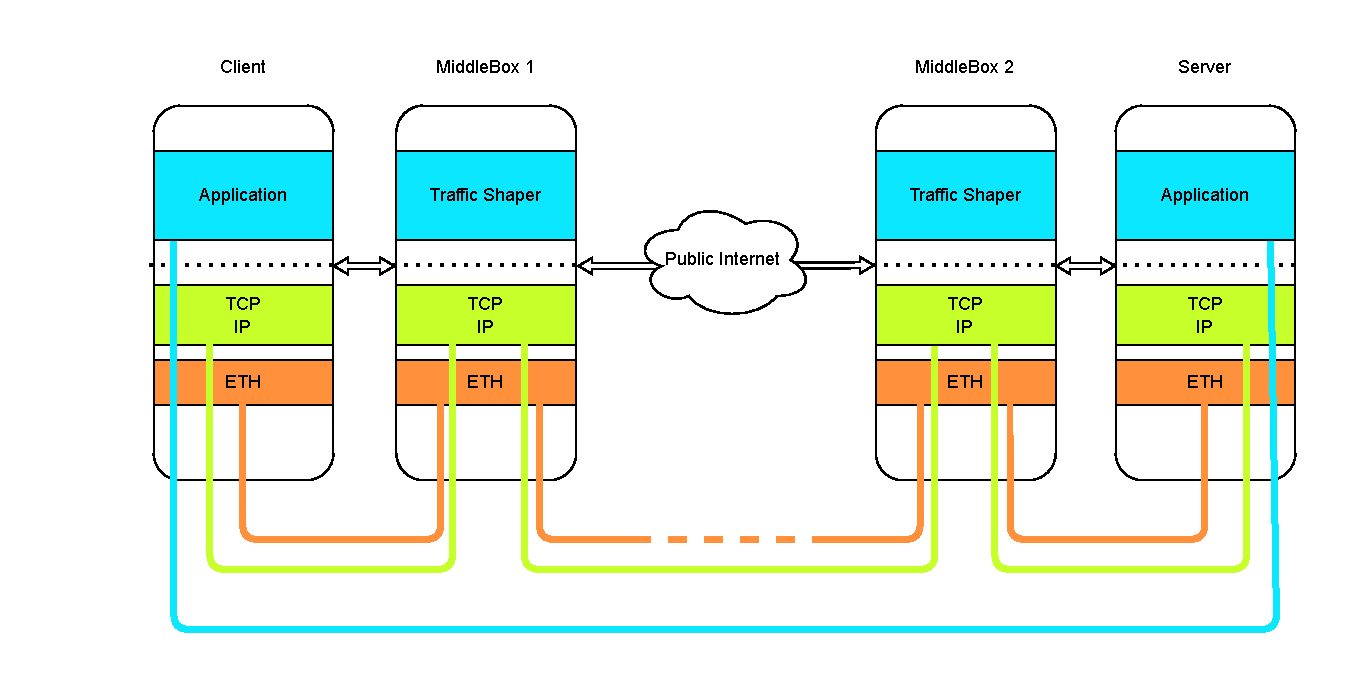
\includegraphics[width=\columnwidth]{figures/design_overview.pdf}
    \caption{End to End design of the {\sys}}
    \label{fig:end-to-end}
\end{figure}

The {\sys} middle-boxes use a reliable connection to transmit control messages.
We define six control messages between middle-boxes: \texttt{conn-req}, \texttt{conn-ack}, , \texttt{conn-est}, \texttt{term-req}, \texttt{term-ack}, and \texttt{term-est}.
Each message contains a message identifier and a flow identifier. 
The {\sys} defines the flow ID as a tuple in the following format: \texttt{flowID=<src\_ip, src\_port, dst\_ip, dst\_port, protocol>}.
In the following sections, we assume the client establishes a TCP connection to transmit data.
Therefore, the \texttt{protocol} value in the flow ID is \texttt{tcp}.
The middle-box stores flows and their states in a specific table called \textit{connection table}.

\subsection{Connection Establishment}
To establish a connection with the server, the client sends a TCP SYN packet.
The middle-box 1 intercepts the SYN packet, extract the flow identifiers, and adds a new row to the \textit{connection table} with the state "connection requested".
The middle-box 1 determines the middle-box at the receiver (middle-box 2 in our case) using the flow ID, and sends a \texttt{conn-req} control message to the middle-box 2.
Upon receiving a \texttt{conn-req} message, the middle-box 2 adds a new row to its \textit{connection table} with the "connection requested" state and uses the flow information to establish a TCP connection with the server on behalf of the client.
Once the connection with the server is acknowledged (i.e. the TCP SYN-ACK packet received from the server), middle-box 2 changes the connection to "connection acknowledged" and sends a \texttt{conn-ack} control message to the middle-box 1.
After receiving the connection acknowledgment, the middle-box 1 also changes the flow state to the "connection acknowledged". 
The middle-box 1 sends SYN-ACK packet to the client to create a connection with the client on behalf of the server.
When the connection with the client is completed, middle box 1 changes the flow state to "established" and sends a \texttt{conn-est} message to the middle-box 2.
The middle-box 2 also changes the flow state to "established" and sends an ACK message to the server.
This procedure is demonstrated in Figure \ref{fig:connection}

\begin{figure}[!htbp]
    \centering
    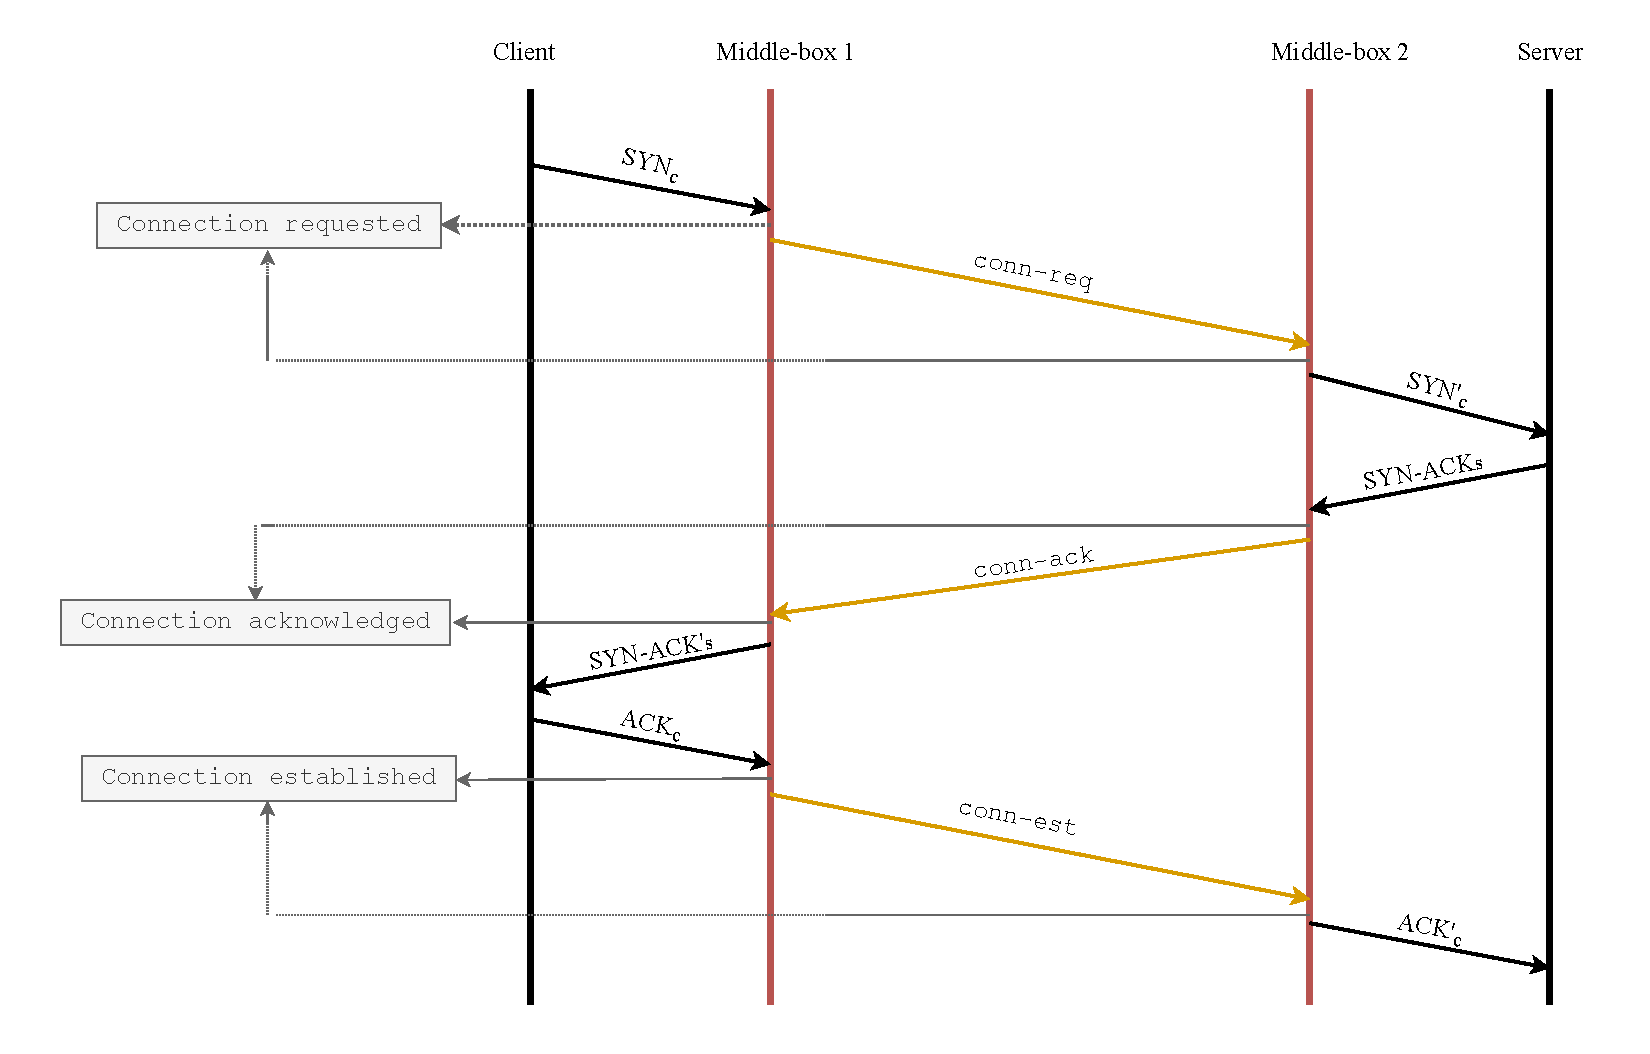
\includegraphics[width=\columnwidth]{figures/connection-establishment.pdf}
    \caption{Time line of connection establishment in {\sys}}
    \label{fig:connection}
\end{figure}
\subsection{Data Transmission}
When the connections with the client and server are established based on the procedure explained in the previous section, middle-boxes create a data channel (e.g. separate TCP connection) to transmit the shaped traffic.
At this point, three independent TCP connections are established for end-to-end traffic transmission.
For every established connection in the connection table, the middle-box creates a dedicated queue named connection private queue. 
Incoming data of the flow is stored in its corresponding queue.
The differentially private traffic shaper determines the size of data that should be moved from the flow private queue to the public queue based on the mechanism described in \ref{subsec:DP-mechanism}. 
If the determined size is larger than the amount of data in the private queue, the data will be padded with dummy data.
The padded traffic is encrypted to make the real traffic indistinguishable from the dummy data.
The middle-box on the sender side transmits the encrypted data to the middle-box on receiver side over the established data channel.
In section \ref{sec:DP-shpaing}, we elaborate on the shaping mechanism and discuss the privacy guarantees of it.
Middle-box 2 receives the encrypted traffic and enqueues it into the public queue.
Then, it decrypts the traffic, drops the dummy, and enqueues the real traffic into the public queue.
The real traffic is transmitted over the TCP connection between the middle-box 2 and the server.


\subsection{Connection Termination}
Upon receiving the TCP FIN packet from the client, the middle-box 1 changes the flow state in the \textit{connection table} to the "termination requested".
The middle-box 1 responds with TCP ACK causing the client to enter FIN\_WAIT\_1 state. 
The data transmission over the data channel between two middle-boxes continues until both private and public queues are emptied.
At this point, middle-box 1 sends a \texttt{term-req} message to the middle-box 2 on the server side.
Once the \texttt{term-req} is received by the middle-box 2, it changes the flow state to "termination requested".
Until both the public and private queues are empty, middle-box 2 continues sending data to the server.
After that, middle-box 2 sends a TCP FIN packet to the server on behalf of the client. 
When middle-box 2 receives the TCP FIN packet from the server, sends \texttt{term-ack} control message to the middle-box 1.
Upon receiving the \texttt{term-ack} message, middle-box 1 changes the flow state to "termination acknowledged" and sends the FIN packet to the client on behalf of the server.
The middle-box waits for the final TCP ACK from the client and when received changes the flow state to "terminated" and sends \texttt{term-est} to the middle-box 2.
The middle-box 2 also changes its flow state to "terminated" and sends the final TCP ACK to the server on behalf of the client, and after that, middle-box 2 terminates the data channel between 2 middle-boxes.
The procedure is represented in Figure \ref{fig:termination}.
\begin{figure}[!htbp]
    \centering
    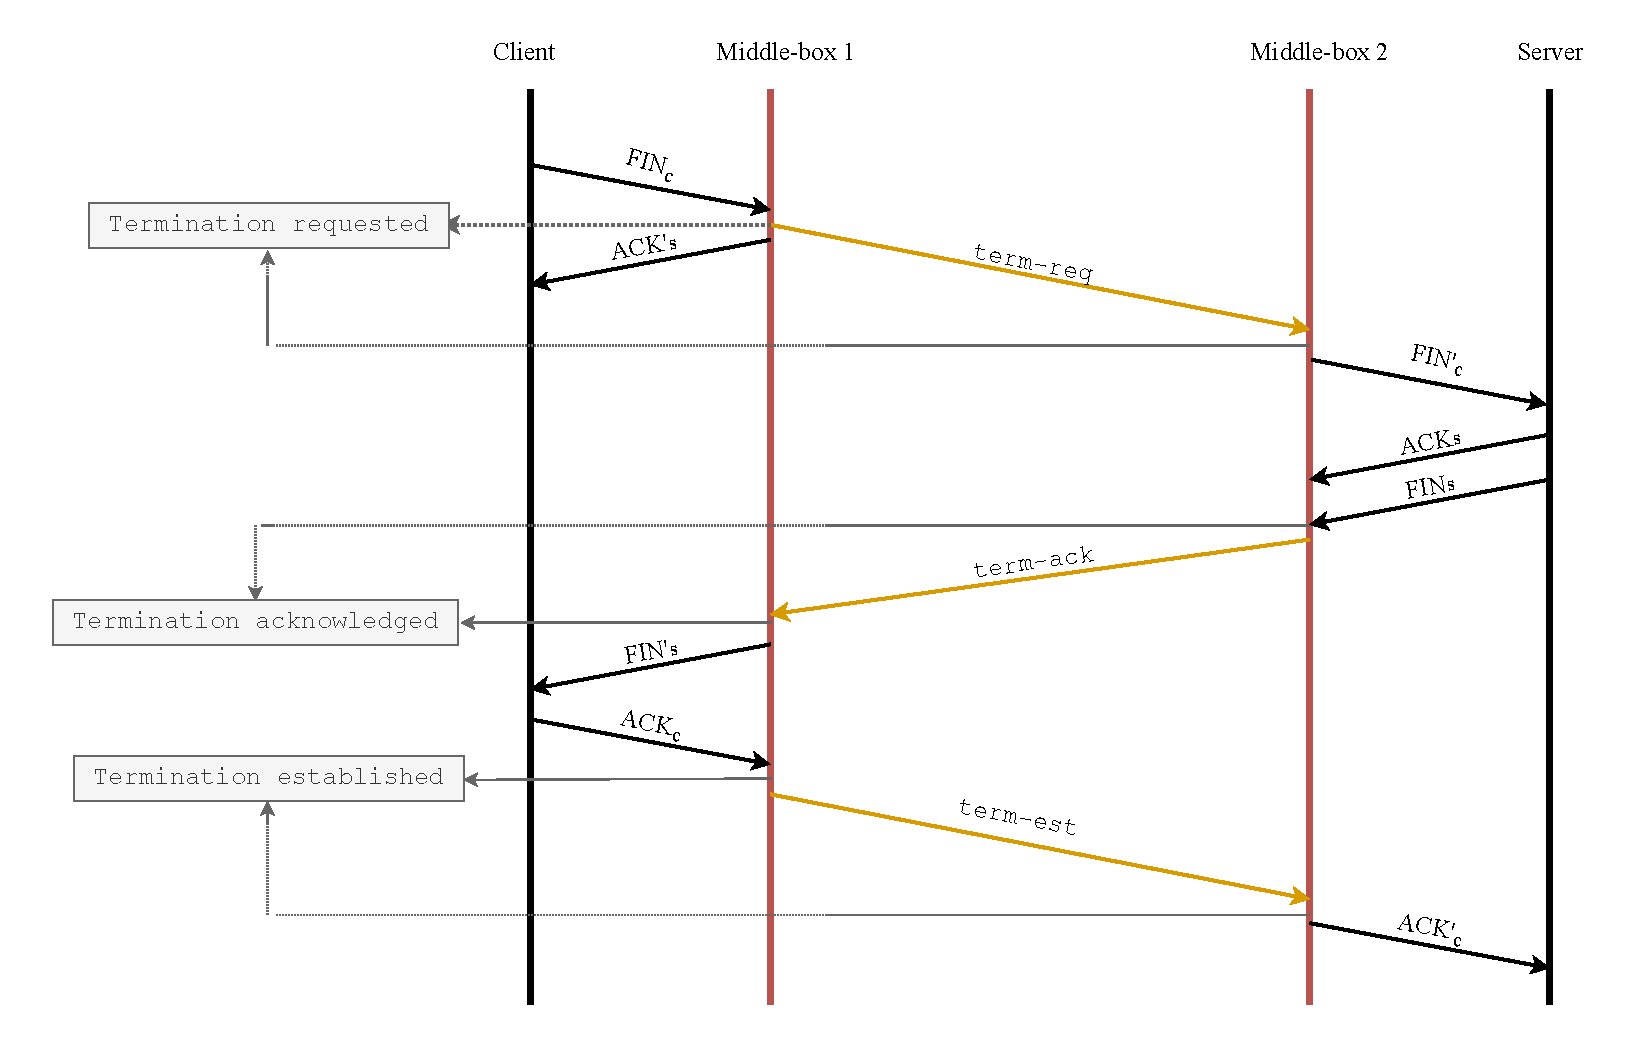
\includegraphics[width=\columnwidth]{figures/connection_termination.pdf}
    \caption{Time line of connection termination in {\sys}}
    \label{fig:termination}
\end{figure}













\begin{algorithm*}[b]
    \DontPrintSemicolon
    \SetNoFillComment
    % \KwIn{$S_N, Q, T, \varepsilon, w, D, min\_burstsize, max\_burstsize$}
    \SetKwFunction{get}{get\_DP\_size}
    \SetKwFunction{send}{send\_data}
    \SetKwProg{Fn}{Function}{:}{}

    \Fn{\get{$Q,\; \varepsilon$}}{
            $D^N = Q + LAP(\frac{D}{\varepsilon})$ \;
            $D^{N}_{clipped} =\max (B_{min}, \; \min (B_{max}, \; D_N))$ \;
            \textbf{return} $D^{N}_{clipped}$ \;
    }
    \Fn{\send{$data\_size,\; dummy\_size,\; MTU$}}{
            $buf[0:data\_size -1] =$ data\_dequeue($data\_size$)\;
            $buf[data\_size:data\_size + dummy\_size -1] =$ dummy\_dequeue($dummy\_size$)\;
            \While{$(buf.size \neq 0)$}{
                    \uIf{$(floor(buf.size/MTU) \neq 0)$}{
                            pkt.payload = $buf$.get\_data(MTU)\;
                          }
                          \Else{
                            pkt.payload = $buf$.get\_data($buf.size$)\;
                          }
                    $buf.size \mathrel{-}=$ sizeof(pkt.payload)\;
                    \tcc{Add DP header to keep track of dummy and real data.}
                    pkt.payload = add\_dp\_header(pkt.payload)\;
                    pkt.payload = encrypt(pkt.payload)\;
                    send\_udp\_pkt(pkt)\;
            }
            \textbf{return} $0$ \;
    }
    %\textbf{SendPacket}(queue\_state, pkt\_size, delay)\;
    \While{(not at end of data transmission)}{
            {sleep}($T$)\;
            $t$ = {get\_current\_time}()\;
            $Q_t$ = {get\_queue\_size}($t$)\;
            $D^S_t$ = \get($Q_t, \; \varepsilon$)\;
            \tcc{Determining the actual data we can send.}
            $D^R_t$ = $\min (Q_t, D^N_t)$\;
            \tcc{Determining the dummy data we need.}
            $D^P_t$ = $D^N_t - D^R_t$\;
            \send$(D^R_t,\; D^P_t,\; MTU)$ \;
    }
    \caption{Middle-Box Timeline}
    \label{alg:middle-box-all}
\end{algorithm*}

%\section{Implementation}
\label{sec:implementation}

\begin{figure}[t]
    \centering
    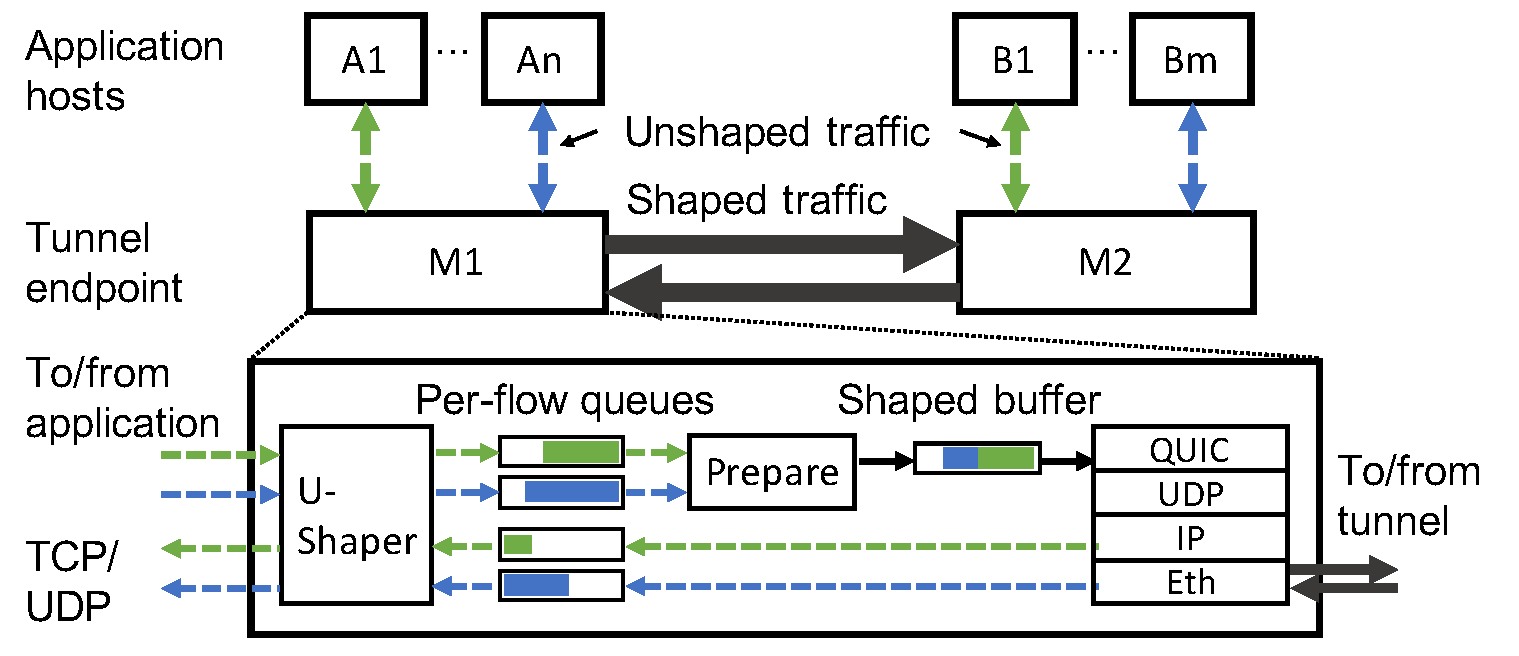
\includegraphics[width=\columnwidth]{figures/middlebox-arch.pdf}
    %    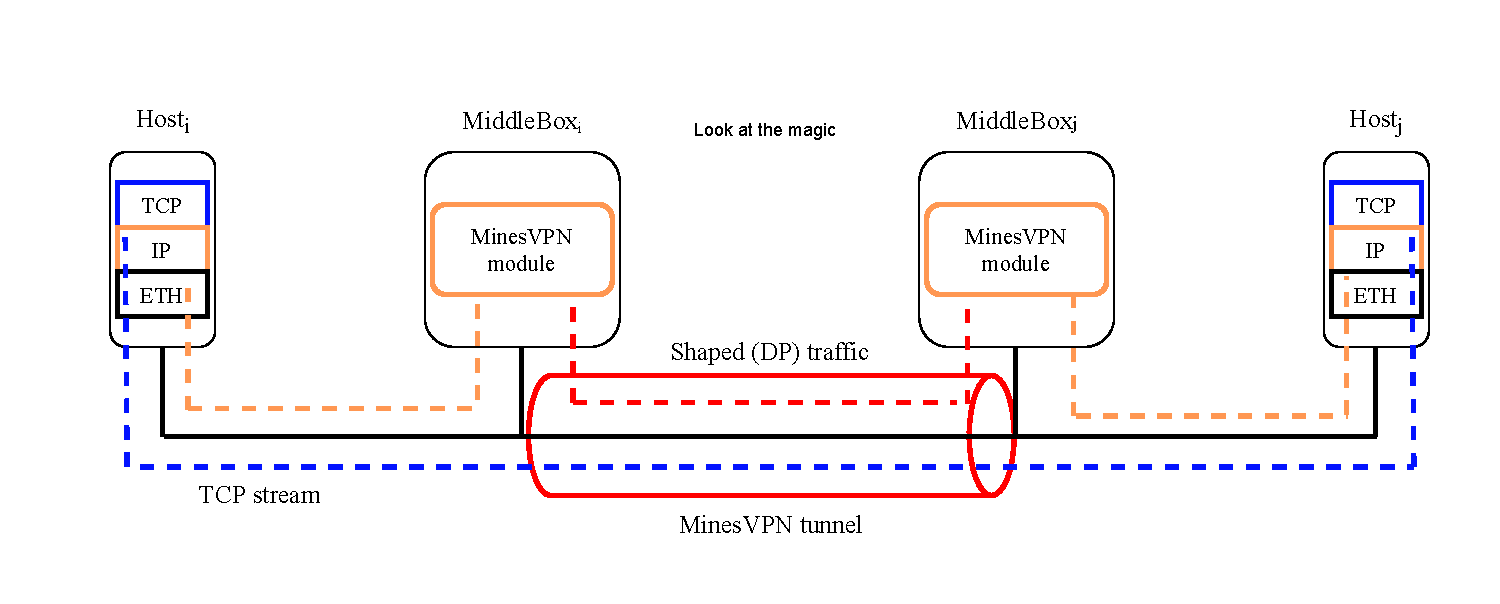
\includegraphics[width=\columnwidth]{figures/design.pdf}
    \caption{{\sys} middlebox design}
    \label{fig:minesvpn-impl}
\end{figure}

We present a middlebox based {\sys} implementation,
as shown in \Cref{fig:minesvpn-impl}.
%
Recall from \S\ref{subsec:key-ideas}, a middlebox can support shaping for
several applications and amortizes~the shaping cost among multiple flows that
share the same tunnel.
Moreover, middleboxes can support multiple ``long-term'' tunnels between
endpoints. Such tunnels may be set up, for instance, between organization
campuses to secure all communication between the campuses without the need for
modifying individual end hosts.

%\begin{table}[t]
%    \centering
%    \renewcommand{\arraystretch}{1.2}
%    \begin{tabular}{lll}
%        \toprule
%        {\bf Outer/Inner} & {\bf TCP} & {\bf UDP}
%        \\
%        \midrule
%        {\bf TCP} & meltdown & inefficient
%        \\
%        {\bf UDP} & insecure & OK
%        \\
%        \bottomrule
%    \end{tabular}
%    \caption{Impact of tunneling a transport inside transport}
%    \label{tab:transport-in-transport}
%\end{table}
%
Following the proxy architecture, the middlebox splits the communication between
two application endpoints over three transport connections:
one between two middlebox endpoints that provides a tunnel and one between
each application endpoint and its local middlebox.
In our implementation, a middlebox consists of two userspace processes,
{\ushaper} for unshaped traffic and {\dshaper} for shaped traffic,
which can run on any standard operating system kernel
and transport stack.
%For each tunnel supported by the middlebox, there is one {\dshaper} process. The
%{\ushaper} process simply multiplexes the flows mapped to all tunnels using one
%or more threads.
Together, the two processes mediate traffic between the application endpoints
and the middleboxes, and sending/receiving shaped traffic to/from the tunnel.
%{\sys}'s prototype relies on a Linux kernel with the standard TCP and UDP
%stack, and the MSQUIC implementation of the QUIC protocol.
%Together the two processes implement the following functionalities: (i)
%establishing tunnels with remote middleboxes, (ii) managing communication
%between local and remote application end points, (iii) moving traffic between
%local application endpoints and the tunnel, (iv) shaping tunnel traffic, and (v)
%providing end-to-end reliable delivery semantics.
We describe each {\sys} component and
how they ensure secret-independent shaping
both within one tunnel and then across multiple tunnels.

\if 0
\subsection{\todo{Middlebox-Middlebox Tunnel Setup}}

%Specifically, the {\dshaper} establishes tunnels with remote middleboxes, shapes
%the outbound traffic on each tunnel according to the tunnel's DP parameters, and
%handles inbound shaped traffic received from the tunnels. The {\ushaper} manages
%the connection with a local application endpoint and mediates the traffic
%between the application endpoint and the {\dshaper}.

%To protect an application's traffic, the middlebox must be placed inside the
%same private network as the application, so that the adversary cannot observe
%the traffic between an application and the middlebox.

%To establish an end-to-end connection, {\sys} relies on three piecewise
%transport connections: one between the two middlebox endpoints that provide a
%tunnel for the application endpoints, and one each between each application
%endpoint and its local middlebox endpoint.

%Each middlebox consists of two userspace processes: a {\ushaper}, which
%interfaces with the local application, and a {\dshaper}, which interfaces
%with the remote middleboxes.
%For each application flow handled by the middlebox, the {\ushaper} mediates
%establishment of the end-to-end connection between the application endpoints,
%and the sending and receiving of traffic from the associated tunnel.
%For this, the {\ushaper} maintains a set of a TCP socket, and a pair of
%transmit and receive queues.
%each application flow to its associated tunnel, sockets, and a pair of transmit
%and receive queues.

%The {\ushaper} shares with the {\dshaper} a {\flowmap} table containing
%mappings of the segments of end-to-end connections, a set of per-flow transmit
%queues, and a set of per-flow receive queues. Together, the two processes manage
%traffic flows on the end-to-end connections.

%\subsection{Shaping Components}
%{\sys} consists of two userspace processes, {\ushaper} and {\dshaper},
%which can run on top of any standard operating system and network stack. The
%{\ushaper} interfaces with the local application endpoints while the {\dshaper}
%process interfaces with the remote middleboxes of the tunnels it handles. The
%{\ushaper} shares the {\flowmap} table, a set of per-flow transmit queues,
%and a set of per-flow receive queues with the {\dshaper}.

%{\sys}'s basic proxy functionality includes setting up a connection between a
%middlebox pair that would carry shaped traffic for sensitive flows, setting up
%and tearing down a connection between the application endpoints for the
%sensitive flows, and  handling congestion. We describe these next.

%\am{de-duplicate from section 5.2, paragraph ``Traffic shaping within a
%    tunnel''.}
%For each tunnel interfacing with a remote middlebox, the {\dshaper}
%maintains a set of a QUIC socket, and a pair of threads, namely {\em Shaper}
%and {\em Shaped\-Receiver} threads.
%For each tunnel interfacing with a remote middlebox, the {\dshaper}
%maintains a set of a QUIC socket, and a pair of threads, namely {\em Shaper} and
%{\em ShapedReceiver}. The Shaper handles outbound traffic while the
%ShapedReceiver handles inbound traffic.


%\paragraph{Middlebox-middlebox tunnel setup.}
A {\sys} middlebox is statically configured with the addresses of the local
application hosts as well as other middleboxes to which the applications’
traffic must be forwarded\footnote{In practice, the middleboxes could discover
other middleboxes using DNS or similar protocols.}.
The {\dshaper} establishes QUIC tunnels with every remote middlebox specified in
its configuration.
%Each tunnel is identified by a 6-tuple consisting of the IP addresses and ports
%of source and destination middleboxes, a reliability flag, and a privacy
%descriptor.
%%{source middlebox IP, destination middlebox IP, source middlebox port,
%%destination middlebox port, reliability flag, privacy descriptor}.
%The reliability flag indicates if the tunnel provides reliable delivery
%semantics or not. The middlebox uses a reliable tunnel for shaping the traffic
%of applications using reliable transport (\eg TCP) and an unreliable tunnel for
%applications using unreliable transport (\eg UDP).
%The privacy descriptor indicates the DP configuration for the tunnel. All
%application flows passing through the same tunnel are subject to the same DP
%parameters.

After a QUIC connection is established between a pair of middleboxes, the
{\dshaper} process in each middlebox initializes three QUIC streams: a control
stream, a dummy stream, and a data stream.
%\todo{fixed number of data streams} that are used to carry the payload of
%application flows.
%The control and dummy streams are designated special stream IDs.
The control stream is used to transmit control messages related to establishment
and termination of the data stream that will subsequently transmit data in the
tunnel. The dummy stream is used to transmit padding in QUIC packets in the
form of QUIC STREAM frames.
%\am{mention reliance on QUIC's encryption protocol.}

%Once a tunnel has been established, each middlebox continuously transmits dummy
%packets at a uniform low rate in the tunnel. \am{Is it uniform as in constant
%shaping or DP shaped? How are we accounting for this overhead?}
%For this, the middlebox establishes a QUIC stream with a special ID, designated
%as the dummy stream, and generates STREAM frames of appropriate length.

\subsection{\todo{End-to-End Connection Management}}
When one application endpoint (\eg A1 in \Cref{fig:minesvpn-impl}) initiates
communication with another application endpoint (B1), the middlebox close to the
initiator (M1) and the responder (M2) work like a forward proxy and a reverse
proxy, respectively.
Together the two middlebox proxies establish a piecewise connection between the
application endpoints.

%\am{Compress to say, connection establishment like a standard forward and
%reverse proxy style.}
%Without loss of generality, we describe the the end-to-end connection
%establishment and termination in the context of a single-client-single-server
%application with one middlebox in front of each (cf.
%\Cref{fig:minesvpn-impl}).  The middleboxes in front of the client and the
%server are called the client middlebox and the server middlebox, respectively.
%
%A flow between a client and a server is carried through a connection that
%consists of three segments: (i) between the client and its middlebox, (ii)
%between the server and its middlebox, and (iii) between the client middlebox and
%the server middlebox. The {\ushaper} in the client middlebox intercepts the
%connection handshake messages from the client and notifies the {\dshaper}.
%The {\dshaper} in the client middlebox sends a handshake message to its peer
%in the server middlebox, which then notifies the {\ushaper} in the server
%middlebox. The {\ushaper} in the server middlebox initiates a handshake with
%the server on behalf of the remote client. When the handshake with the server is
%complete, the server middlebox responds to the client middlebox, which then
%completes the handshake with the client.

Once the connection is established, each application endpoint may send to the
{\ushaper} in its local middlebox an optional shaping configuration
request, which indicates the choice of DP parameters and/or latency constraints
it wishes to use for shaping its outbound
traffic\footnote{Before forwarding the DP parameters to their respective
middleboxes, the applications run an additional handshake protocol after
connection establishment to negotiate the parameters for the traffic between
them.}.
%
Finally, the {\ushaper} sets up an entry in a local {\flowmap} table to establish
shaping for the application endpoints.
%mapping the three connection segments, the associated socket and per-flow
%transmit and receive queues, and the DP parameters for traffic shaping that were
%provided by the application endpoints at the time of flow registration.
%\am{deduplicate from the overview.}

%\paragraph{End-to-end connection shutdown.}
Closing an end-to-end connection follows a similar process as connection
initiation. The {\ushaper} in each middlebox mediates the connection termination
and removes the connection entry from its {\flowmap} table.
%The {\ushaper} in a middlebox intercepts connection termination handshake
%from a client (or server); the {\dshaper} in the middlebox then relays
%connection termination to the {\dshaper} in its peer middlebox; the {\ushaper}
%process on the peer middlebox terminates connection with the corresponding
%server (or client) and responds to the initiating middlebox, which then closes
%the connection with its local node.
%Finally, both middleboxes remove the connection entry from their local
%{\flowmap} tables.
\fi

\subsection{Components}
\label{subsec:impl-mediation}
\paragraph{UShaper.}
The {\ushaper} mediates the unshaped traffic between one or more local
application endpoints and the {\dshaper} using per-flow transmit and receive
queues.
It implements a transport server (or client) for interfacing with each local
client (or server, respectively) application endpoint\footnote{The {\ushaper}
supports both UDP and TCP endpoints for applications.}.
%The type of the transport endpoint depends on the application's choice of
%transport protocol.
Additionally, it shares a {\flowmap} table with the {\dshaper},
which consists of an entry for each end-to-end flow. Each entry maps the
piecewise connections with
%the associated sockets of {\ushaper} and {\dshaper}, a
the pair of transmit and receive queues to carry the local application's byte
stream, and shaping configurations (\eg privacy descriptor) provided by an
%\todo{(\eg privacy descriptor, tunnel lifetime)} provided by an
application at the time of flow registration.
%The transmit queues of the end-to-end flows mapped to a single tunnel connection
%correspond to the tunnel's buffering queue, on which tunnel's DP guarantees
%rely.

The {\ushaper} receives the outbound traffic from a sender application
and enqueues the byte stream into a per-flow transmit queue shared with the
{\dshaper}.
It also dequeues bytes from a per-flow receive queue, repackages them
into transport packets and sends them to the receiver application.
%It also dequeues QUIC packets from a
%%the corresponding
%per-flow receive queue, discards the dummy frames, repackages the payload from
%the remaining frames into transport packets and writes them to the socket of
%the application flow.

%\if 0
\begin{figure}[t]
    \centering
%    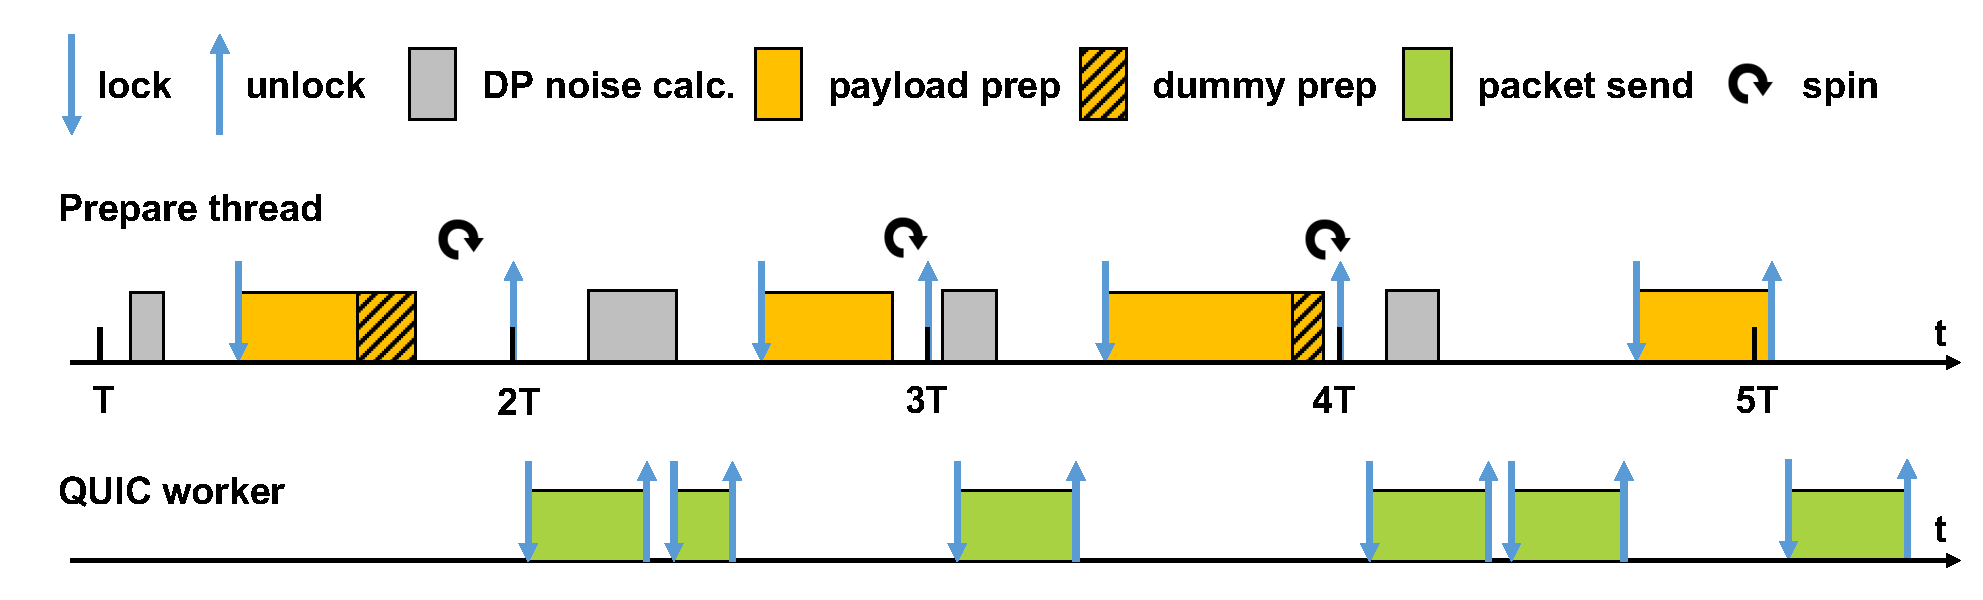
\includegraphics[width=\columnwidth]{figures/schedule.pdf}
    \includegraphics[width=\columnwidth]{figures/schedule5.pdf}
    \caption{{\dshaper} schedule}
    \label{fig:middlebox-schedule}
\end{figure}
%\fi

\paragraph{DShaper.}
%\label{subsec:impl-shaping}
%\am{The description does not match the security spec and will be replaced with
%the alternate text once an implementation satisfying the spec is confirmed.}
%\paragraph{Traffic shaping.}

The {\dshaper} process consists of a {\prepare} thread and a QUIC
worker thread.
The {\prepare} thread instantiates a QUIC client/server to establish
a tunnel with the remote middlebox and implements the DP shaping logic.
%On~the transmit side, {\prepare} examines the number of bytes in each
%per-flow transmit queue, determines the number of bytes to transmit,
On the transmit side, {\prepare} \update{prepares shaped buffers based on DP
measurements of the transmit queues}
and then submits shaped buffers to the QUIC worker.
On the receive size, the QUIC worker transmits ACK frames to the sender
and then decrypts the QUIC packets, extracts the STREAM frames, and copies
bytes (including dummy bytes) from each frame into the appropriate per-flow
receive queue.



%The {\dshaper} implements a thread, named {\prepare}, which instantiates a QUIC
%client/server to establish a tunnel with a remote middlebox, as well as the
%DP~shaping logic. The {\dshaper} links the QUIC library, which implements a
%worker thread that receives shaped buffers from {\prepare} and transmits them as
%one or more QUIC packets.
%\mis{I found this quite difficult to parse and want to suggest
%an alternative,
%but I was not 100\% sure that I understood the implementation well enough
%to get this right, so I'm putting it in a comment.
%The {\dshaper} process consists of a single {\prepare} thread and one
%or more QUIC worker threads.
%The {\prepare} thread both instantiates a QUIC client/serer to establish
%a tunnel with the remote middlebox and implements the DP-shaping logic.
%On the transmit side, {\prepare} examines the number of bytes in each
%per-flow transmit queue, determines the number of total bytes to transmit,
%and then submits DP-shaped buffers to the QUIC worker threads.
%On the receive size, QUIC worker threads rtansmit ACK frames to the sender
%and then decrypt the QUICK packets, extract the STREAM frames, and copy
%bytes (including dummy bytes) from each frame into the appropriateper-flow
%receive queue.
%}

%{\prepare} implements a periodic loop of length $T_{prep}$ that runs until the
%end of the tunnel lifetime.
%{\prepare} implements a while loop that runs until the end of the tunnel
%lifetime, which mainly follows the design from \S\ref{subsec:design-overview} to
%transmit shaped packets.
%After periodic intervals of length $T_{prep}$, it computes a
%differentially-private transmission size $S$ and prepares a transmit buffer of
%the same length to be sent out over QUIC.
%In each loop iteration, it prepares a transmit buffer of a
%differentially-private size $\qlendp$ to be sent to QUIC.
%{{\prepare} iterates through the transmit queues mapped to the tunnel; it
%dequeues a number of payload bytes from the queues that is the minimum of
%$\qlendp$ and the available bytes on the queues and appends them to the transmit
%buffer.}
%If the total number of payload bytes available across all transmit queues is
%lower than $\qlendp$, {\prepare} further appends dummy bytes for the remaining
%length of the transmit buffer.
%Finally, {\prepare} enqueues the transmit buffer to QUIC.

%The QUIC worker generates QUIC STREAM frames using the bytes from the
%appropriate streams passed in the transmit buffer, and then packages the STREAM
%frames into one or more QUIC packets. Finally, {the QUIC worker}
%encrypts the QUIC packet and forwards it to the underlying UDP layer, which
%ultimately transmits the packets at link speed.

%%%%%%%%%%%%%%%%%%%%%%%%%%
%%% Correct implementation
%%%%%%%%%%%%%%%%%%%%%%%%%%
%The {\dshaper} iterates through the transmit queues mapped to the tunnel; it
%dequeues a number of payload bytes from a transmit queue that is minimum of $S$
%and the available bytes on the queue, packages them into a QUIC STREAM frame,
%and appends the frame to the transmit buffer. If the total number of payload
%bytes available across all transmit queueus is lower than $S$, the {\dshaper}
%further enqueues a dummy frame of length $S - P$, where $P$ is the total number
%of payload bytes dequeued from the transmit queues. Finally, the {\dshaper}
%forwards the buffer to QUIC, which encapsulates the buffer into a QUIC packet,
%encrypts it, and then forwards it to the underlying UDP layer, which ultimately
%transmit the packet at link speed.
%At periodic intervals, the Shaper computes a differentially-private transmission
%size $S$, dequeues a number of payload bytes $P$ from the transmit queue, where
%$P$ = $min$($S$, total bytes in queue), and packages them into a QUIC frame. The
%Shaper also prepares a frame with a number of dummy bytes $D$ = $S - P$.
%Finally, the Shaper packages the payload and dummy frames into a single QUIC
%packet, encrypts the packet, and forwards the packet to the underlying UDP
%layer, which ultimately transmits the packet at link speed.

%The {\prepare} and QUIC worker threads follow the design from
%\S\ref{subsec:design-overview} to transmit shaped packets.
%When shaped QUIC packets arrive from a tunnel, QUIC transmits
%an ACK frame as a response to the sender, decrypts the received QUIC
%packets, extracts the STREAM frames, and copies the bytes (including dummy) from
%each frame into the appropriate per-flow receive queues shared with the
%{\ushaper} process.
%The {\ushaper} handles the packets as discussed in
%\S\ref{subsec:impl-mediation}.
%The {\dshaper} decrypts each inbound QUIC packet received from a tunnel and
%places
%the packet in a per-flow receive queue shared with the {\ushaper} process. QUIC
%also transmits an ACK frame as a response to the sender.
%\todo{Note that the ACK frames are themselves not subject to DP shaping.}

\if 0
%%%%%%%%%%%%%%%%%%%%
%% no longer needed?
%%%%%%%%%%%%%%%%%%%%
\paragraph{\todo{Prioritizing payload over dummy.}}
Note that %Recall that
{\prepare}'s payload preparation logic executes once at the beginning of every
interval of length $T_{prep}$.
%, \eg at time $t$, $t + T_{prep}$, $t + 2T_{prep}$, and so on.
Consider a scenario where an application's payload is
enqueued in a transmit queue at a small time $\theta$ after
the {\prepare} thread checked the transmit queue for payload bytes at the
beginning of interval $k$.
%$kT_{prep}$.
%In this case, there is no application data to transmit during the
%interval $[kT_{prep}, (k+1)T_{prep})$.
%{\prepare} will transmit dummy bytes in the interval $[kT_{prep},
%(k+1)T_{prep})$, while the application
%payload will be delayed by at least $T_{prep}$ and will be transmitted during
%the next interval $[(k+1)T_{prep}, (k+2)T_{prep})$.
{\prepare} will transmit dummy bytes in the interval $k$, while the
application payload will be delayed by at least $T_{prep}$ and will be
transmitted during the next interval ${k+1}$.
To reduce the transmission latency for the application, {\sys} modifies the
implementation of {\prepare} such that it can prioritize
payload bytes over dummy bytes more frequently.

{\prepare} implements a higher frequency loop with interval $T_{dequeue}$ inside
the
loop with interval $T_{prep}$. It splits the DP size decision generated at the
beginning of $T_{prep}$ into $T_{prep}/T_{dequeue}$ smaller uniform sizes and
prepares smaller transmit buffers by checking the transmit queue once at the
beginning of every $T_{dequeue}$ interval.
%\am{Revisit based on final design and experiments.}
\fi

%When the {\DPlogic} computes the size for the next burst transmission, it places
%a token in a local {\tokenq} rather than immediately dequeueing bytes from
%{\txq}. The packetizer, which is now decoupled from the {\DPlogic}, periodically
%checks the {\tokenq}. If the {\tokenq} is non-empty, it dequeues payload and
%dummy bytes appropriately from {\txq} to prepare a buffer of size determined by
%the first dequeued token; otherwise, the packetizer goes to sleep.
%
%The intervals of the {\DPlogic} and the packetizer determine a tradeoff between
%transmission latency for payload bytes and the bandwidth overhead due to dummy
%bytes.
%Optimally, the packetizer interval must be smaller than the {\DPlogic} interval,
%while the {\DPlogic} interval must align with the application traffic rate.
%However, the {\DPlogic} interval must not be highly reactive to the application
%traffic rate as it could reveal application secrets.
%In practice, {\sys} would incur low overheads when the traffic has a stable
%burst rate.
%%\todo{TODO}

%\paragraph{Privacy aggregation and flow prioritization.}
%{\sys} allows clients to configure the tradeoff between their individual privacy
%and overheads.
%%In principle, {\sys} provides DP guarantees individually for each application
%%flow.
%In principle, {\sys} can shape each application flow through an independent
%tunnel with per-flow DP guarantees. However, if several application endpoint
%pairs use the same middleboxes as tunnel endpoints, they can choose to amortize
%their overheads by sharing a tunnel and their DP privacy budget.
%%However, clients using the same tunnel can choose to amortize their overheads
%%by sharing their privacy budget.
%Additionally, they may provide a prioritization factor to allow {\sys} to select
%payload bytes from their per-flow queues in order of their priority. Clients can
%notify their middlebox about their desired privacy guarantee and prioritization
%factor using the privacy configuration protocol.
%
%To shape multiple flows through a shared tunnel, a {\dshaper} initializes a
%fixed
%number of data streams in the tunnel connection. When the {\ushaper} receives a
%new
%application flow, it adds a mapping for the application connection, and a pair
%of transmit and receive queues with the shared tunnel connection. Upon receiving
%a privacy configuration message, the {\ushaper} updates the configuration of a
%flow. Subsequently, at each interval, the {\dshaper} process selects payload
%bytes
%by iterating through the per-flow queues belonging to the same privacy class in
%order of the queues' priority.

\subsection{Ensuring Secret-Independent Shaping}
\label{subsec:impl-shaping-security}
%\Cref{fig:middlebox-schedule} illustrates the schedule of operations on
%{\prepare}
%and QUIC worker threads on the outbound path.
%The green and orange boxes represent data-independent and data-dependent
%operations, respectively.
The goal of the middlebox is to ensure that {\em an adversary observes
$\qlendp$ bytes in each transmit interval $\dpintvl$.}

Let's first understand the factors that might prevent the middlebox from
guaranteeing this property.
Even though an application is physically isolated from the middlebox and can
encrypt its data (\eg using end-to-end TLS), its flow control behavior could be
secret-dependent and could affect the middlebox's execution.
For instance, the presence or absence of payload traffic from an application
can affect the time {\dshaper} requires to prepare the shaped buffers.

Ensuring the high-level goal mentioned above requires that
(i) {\prepare} computes $\qlendp$, allocates and prepares a buffer of length
$\qlendp$, and passes the buffer to the QUIC worker within $\dpintvl$,
(ii) the QUIC worker prepares encrypted packets from the buffer and sends them
to UDP, such that the total payload size of the QUIC packets prepared in
$\dpintvl$ is $\qlendp$, and
(iii) the UDP stack transmits the packets totaling to $\qlendp$ bytes of payload
size to the NIC in $\dpintvl$.
Enforcing all these properties would produce a strict time-trigggered schedule
for each component, which would significantly reduce link utilization and
increase packet transmission latencies.
%Moreover, the value of $\dpintvl$ required would be large to account for
%potential secret-dependent (\eg flow control) as well as secret-independent
%delays (\eg congestion control).
%This would significantly increase packet transmission latencies.

{\dshaper} instead provides the following guarantees. (See
\Cref{fig:middlebox-schedule} for reference.)
%The {\dshaper} provides two guarantees.
First, {\prepare} \update{guarantees that a DP measurement $\qlendp$ is performed
every fixed time interval $\dpintvl$}.
Secondly, {\prepare} guarantees that a shaped buffer of length $\qlendp$ is {\em
prepared} within a fixed time $\dpintvl_{prep}$.
Thirdly, {\prepare} locks the shaped buffer for a fixed time,
$\dpintvl_{enq}$, during which it enqueues the shaped buffer for a QUIC
worker.
This ensures that the buffer is completely enqueued before QUIC starts
transmitting it and that
QUIC receives the buffer only at fixed delays.
%\todo{
We empirically profile the time taken by {\prepare} for preparing and enqueueing
shaped buffers for various DP lengths. We set $\dpintvl_{prep}$ and
$\dpintvl_{enq}$ to maximum values determined from profiling, and $\dpintvl$ to
the sum of these maximum values. If {\prepare} takes time less than
$\dpintvl_{prep}$ (or $\dpintvl_{enq}$, respectively) to prepare (or enqueue) a
shaped buffer, it sleeps until the end of the interval before moving to the next
phase.
%}
%\todo{We empirically profile the maximal time $\dpintvl^{max}_{prep}$ and
%$\dpintvl^{max}_{enq}$ taken by {\prepare} for preparing and enqueueing shaped
%buffers for various DP sizes. We set $\dpintvl_{prep} = \dpintvl^{max}_{prep}$,
%$\dpintvl_{enq} = \dpintvl^{max}_{enq}$, and $\dpintvl = \dpintvl^{max}_{prep} +
%\dpintvl^{max}_{enq}$. If {\prepare} takes time less than
%$\dpintvl^{max}_{prep}$ (or $\dpintvl^{max}_{enq}$, respectively),
%to prepare (or enqueue) a shaped buffer,
%it sleeps until the end of the interval before moving to the next
%phase.}
%\am{Too symbol heavy?}


%{\dshaper} instead provides two guarantees.
%%The {\dshaper} provides two guarantees.
%First, {\prepare} guarantees that each shaped buffer is {\em prepared} within a
%fixed time interval $\dpintvl$.
%\todo{For this, we empirically profile the maximal time taken $\dpintvl_{max}$
%by {\prepare} until
%buffer preparation for various DP sizes and set $\dpintvl$ to this
%$\dpintvl_{max}$. If {\prepare} takes lesser time than $\dpintvl_{max}$ to
%prepare a transmit buffer, it sleeps until the end of the interval, at which
%point it starts enqueueing the buffer to QUIC.}
%Secondly, QUIC's packetization remains data-independent. For this, {\prepare}
%synchronizes with the QUIC worker on the the transmit buffers,
%%the preparation of buffers to be transmitted,
%ensuring that QUIC cannot receive fewer bytes than the computed DP
%size of the interval before it sends packets to the network. F

In the middlebox, {\prepare} and QUIC worker threads run on a separate cores
sharing only the shaped buffers.
{\ushaper} runs on yet a differnet core, shares only the
{\flowmap} and the per-flow queues with {\dshaper}.
Variations in {\prepare}'s execution due to the state of the
per-flow queues are hidden by $\dpintvl_{max}$, while QUIC's
execution depends only on shaped buffers and thus, is secret-independent.
Consequently, the packetization of shaped buffers in the QUIC worker and the UDP
stack is secret-independent and any variations in packet transmit times induced
due to their execution constitute post processing noise.

A remaining concern could be leaks via internal side channels in the middlebox
that cause {\dshaper} to fail to prepare the expected amount of data within a
scheduled interval.
For instance, {\dshaper}'s execution could be influenced by microarchitectural
state (\eg caches, memory and PCI buses, write buffers, interrupts) based on the
application's flow control.

\if 0
A remaining concern could be leaks via internal side channels in the middlebox
that cause {\sys} to fail to transmit the expected amount of data within a
scheduled interval. Even though an application is physically isolated from the
middlebox and may encrypt its data (\eg using TLS for the end-to-end
connection), the application’s flow control could be secret-dependent and could
affect {\sys}'s execution.

\todo{For instance, flow control affects the number of payload bytes available
for transmission and, consequently, the amount of padding that may be added to a
segment. Processing payload and dummy bytes could take different amounts of
time.} Secondly, the execution of the Shaper could be influenced by interrupts
or microarchitectural state (\eg caches, memory and PCI buses, internal write
buffers) based on the presence or absence of payload traffic from the
application.
\fi

We have not been able to exploit such side channels to identify traffic content.
Nevertheless, such side channels could be eliminated via resource partitioning,
performance isolation, and constant-time implementation techniques
\cite{liu2016catalyst, coppens2009practical, zhang2011predinteractive,
    almeida2016verifying}.



\subsection{Scheduling Across Tunnels}
{When transmitting traffic on multiple tunnels, {\sys} must ensure that the
unshaped traffic of one tunnel is not leaked to another tunnel. For this, {\sys}
must isolate the tunnels from each other in the middlebox.
%Based on \S\ref{subsec:impl-shaping-security}, we require that the {\prepare}
%and QUIC worker threads must be performance isolated from {\ushaper} in each
%tunnel, (ii) the timing of {\prepare} must be masked to secret-independent
%times.
Thus, {\sys} partitions the middlebox cores into three groups, each core group
hosting the {\ushaper} process, the {\prepare} threads, and the QUIC worker
threads from different tunnels.
Furthermore, {\sys} uses a TDMA schedule among the {\prepare} threads, while
\update{padding} each thread's execution to a secret-independent time.
%In {\sys}, only the {\dshaper} components need to be isolated. {\sys} uses a
%TDMA to schedule the {\dshaper} processes of different tunnels.
Since each {\prepare} thread enqueues shaped buffers at secret-independent
times, the QUIC workers can subsequently package the buffers into packets and
transmit the packets across multiple tunnels following any arbitrary schedule.}
%
{Determining optimal TDMA schedules and their adaptation to the changing
number of active tunnels is left to future work.}

\if 0
%\paragraph{Shaping outbound traffic.}
\subsection{Reliable Delivery}
\am{Explain how this is relevant to security.}
Applications relying on TCP expect reliable delivery guarantees. Thus, {\sys}'s
middlebox needs to support flow control, congestion control, and loss recovery
to enable reliable delivery across the piecewise connections.

%\paragraph{Between an end host and a middlebox.}
For a connection between an end host and the middlebox, flow control, congestion
control, and loss recovery are handled by the transport layer protocol used on
the connection as usual.
%
%\paragraph{Between two middleboxes.}
For a tunnel connection, the QUIC protocol handles flow control, congestion
control, and loss recovery in
the tunnel.
%In case of congestion or packet losses on the network carrying the tunnel
%traffic,
QUIC buffers the prepared outbound packets until they are acknowledged and
retransmits unacknowledged packets in case of packet losses. The buffered
packets contain traffic whose size and timing have been shaped; therefore,
additional delays due to network congestion or packet losses only add noise to
an adversary’s observations and do not affect application’s privacy.

%\paragraph{Impact of prolonged network instability.}
In case of prolonged congestion or losses, or if the receiver is overwhelmed for
an extended period of time, QUIC's buffers in the sender middlebox may overflow
and drop packets.
The sender middlebox must then apply a back pressure on its local end hosts to
force them into slowing down their transmissions. MinesVPN’s middlebox
implements the back pressure mechanism as follows. When the {\dshaper}'s QUIC
buffer overflows, it stops dequeueing payload bytes from the per-flow transmit
queue. This causes the transmit queue to fill up and prevents the {\ushaper}
from enqueueing more bytes into the queue, which in turn causes the {\ushaper}
process to not read bytes from the TCP socket interfacing with the application.
Consequently, TCP notifies the sender of a reduction in the receive window
causing the sender to slow down transmission. Eventually, TCP's buffers may fill
up and cause TCP to drop incoming packets from the application, ultimately
notifying the sender application's TCP stack of congestion.

The system recovers from congestion once {\dshaper} receives
acknowledgements for transmitted packets and can dequeue payload
bytes from the transmit queues\footnote{{\sys} could expedite congestion
notification to the sender application by using mechanisms, such as explicit
congestion notification \cite{ecn}. We leave a detailed analysis of congestion
handling to future work.}.

A remaining challenge arises when a sender middlebox acknowledged payload bytes
from the local sender application, but is forced to drop the bytes due to
instability on the tunnel network. This violates the reliable delivery semantics
expected by the application. Note that existing proxies face a similar challenge
too. {\sys} does not aggravate the issue and, therefore, similar to other
proxies, leaves the resolution to the application and the user.
%\am{Dealing with bytes acknowledged by middlebox but no longer able to buffer.}
%\todo{Recovery from congestion.}
\fi

%\subsection{Scheduling across tunnels.}
%Once the traffic within each tunnel is shaped, sending and receiving traffic
%across multiple tunnels can follow any schedule.





%%%%%
%%%%%
\if 0
The middlebox consists of two VMs: host-facing ({\unshapedVM}) and
tunnel-facing ({\shapedVM}). Each VM hosts a separate network stack, which
consists of a transport layer on top of a
network layer on a top of an ethernet layer. The {\unshapedVM} supports one or
more transport protocols, such as TCP, UDP, and QUIC.
The {\shapedVM} primarily relies on UDP but additionally runs three layers atop
UDP: a {\DPlogic} on top of an encryption layer, which is integrated with the
QUIC protocol~\cite{langley2017quic}\footnote{In principle, the {\shapedVM} could use
TCP as a
    reliable tunnel transport; however, we choose QUIC for \todo{reasons of efficiency and
        ease of implementation}.}.
%because it enables efficient multiplexing of multiple client streams, avoids
%head-of-line blocking,

The {\unshapedVM} receives unshaped traffic from an
end-host application and forwards it to the {\shapedVM}. The {\DPlogic} shapes
the traffic according to DP and transmits it over a QUIC connection. In the
reverse direction, the {\shapedVM} forwards the traffic received over the QUIC
connection to
the {\unshapedVM}, which in turn forwards it to the target application after
decryption and removing any padding.

We now elaborate on the interaction between an end-host application and a
middlebox, as well as the components of the middlebox.

\subsection{\unshapedVM}
%
%The {\unshapedVM} places an application's outbound bytes, including handshake
%and control packets, in the transmit queue, which are dequeued and shaped in the
%{\shapedVM}. Similarly, the {\shapedVM} places inbound packets from the tunnel
%in the receive queue, which are dequeued in the {\unshapedVM}, decrypted,
%stripped of padding, and forwarded to the appropriate end-host application.

The {\unshapedVM} contains a userspace application,
called the {\mediator}, and a small kernel module, which interact via another
FIFO queue in a shared memory region.
The kernel module maintains the {\flowmap}, which consists of the
mapping of the segments of each end-to-end connection and other configuration
parameters for the connection.
In addition, the {\mediator} interfaces with the {\shapedVM} via statically sized lockfree FIFO
queues. For each end-to-end connection, there is a pair of transmit and receive
queues allocated in a shared memory region between the VMs.

When the middlebox receives a new flow from an end host application, the kernel
module in the {\unshapedVM} intercepts the handshake messages, copies them into
the FIFO queue shared with the {\mediator} and responds to the end host in
accordance with the transport protocol.  The {\mediator} forwards the handshake
messages to the {\shapedVM}, which handles the remaining stages of the
end-to-end connection establishment with the remote peer and returns information
of the later connection segments to the {\mediator}. The {\mediator} forwards
the connection information to the kernel module, which then populates a
{\flowmap} entry for the end-to-end connection.

Once a connection is established, the kernel module also intercepts the data
packets of the end host's transport protocol, copies them into the FIFO queue
shared with the {\mediator}, and sends appropriate responses to the end host in
accordance with the transport protocol.
Furthermore, the {\mediator} decrypts packets from the receive queue, strips off
any padding, and forwards the payload bytes to the kernel module. The kernel
module encapsulates the payload with protocol headers and forwards
the packets to the appropriate end hosts.

\subsection{\shapedVM}
The {\shapedVM} implements the core of {\sys}'s traffic shaping design.
The {\shapedVM} establishes a bidirectional QUIC connection with the
{\shapedVM} in each of its peer middleboxes. Within each connection, the
{\shapedVM} further opens a \todo{bidirectional} QUIC stream with its peer,
which is assigned the stream ID 0 and is used as a stream for dummy byte
transmissions.
\todo{TODO: Complete the section}
\fi

%\begin{figure*}[t]
%\center{
    %%    \centering
    %    \subfigure[Time line of connection establishment in {\sys}] {
        %%    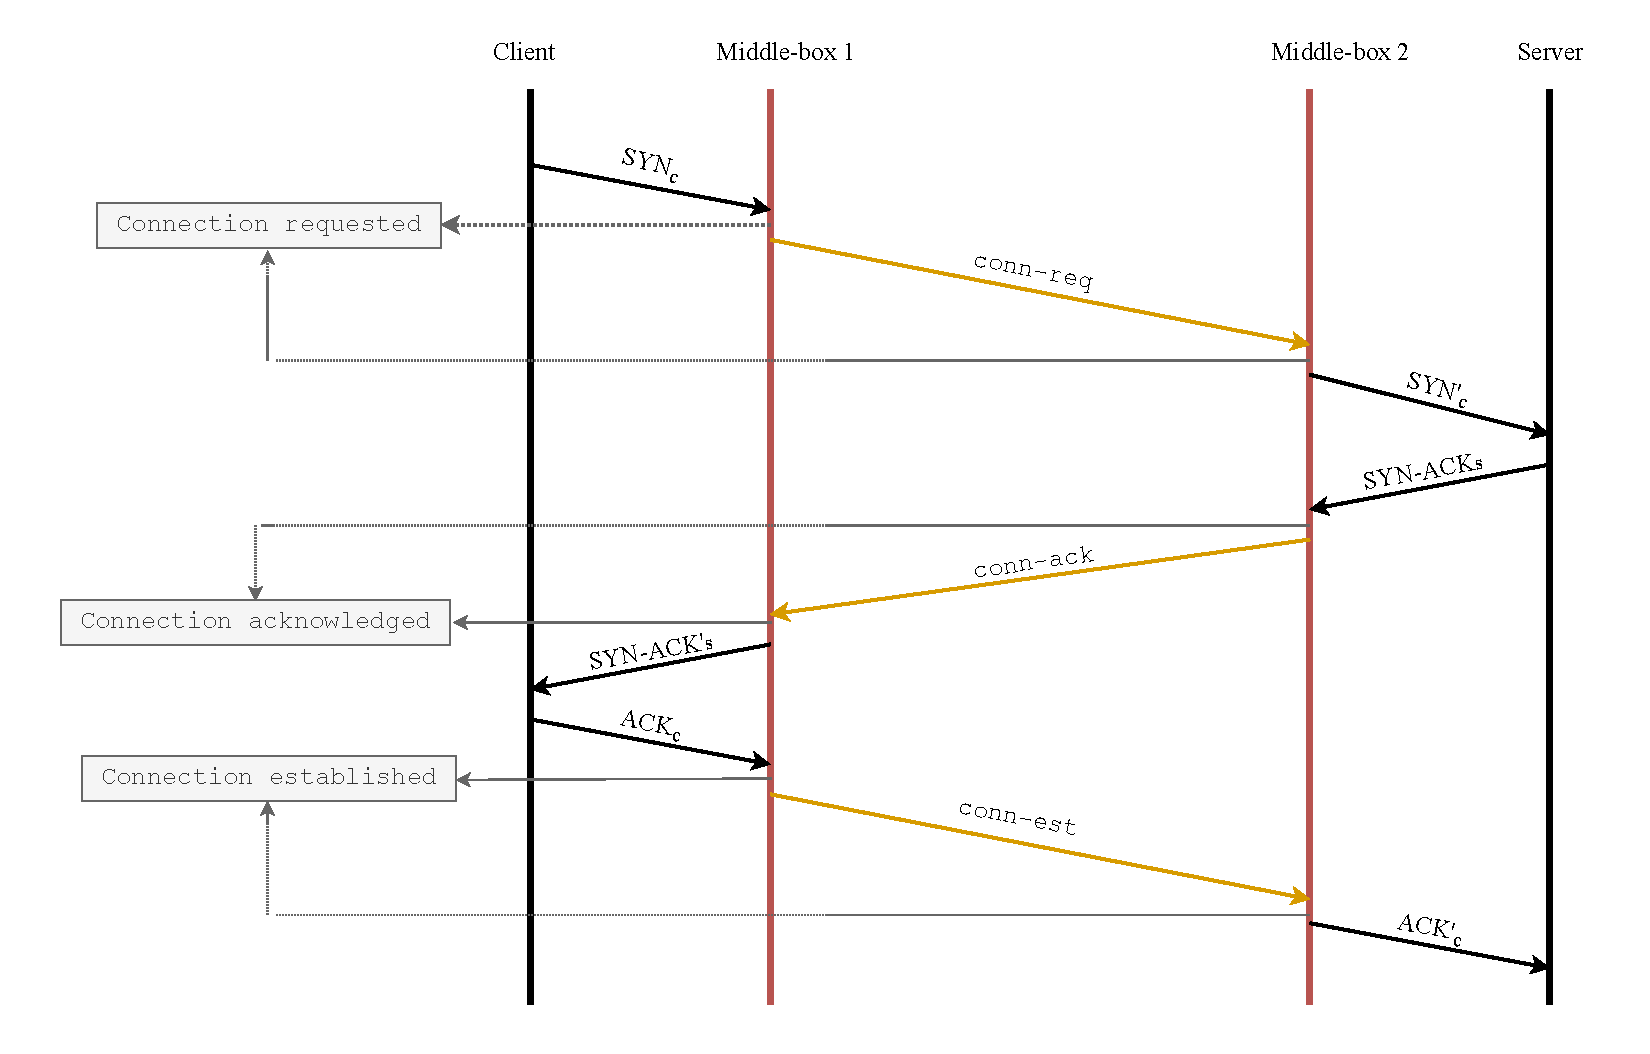
\includegraphics[width=\columnwidth]{figures/connection-establishment.pdf}
        %    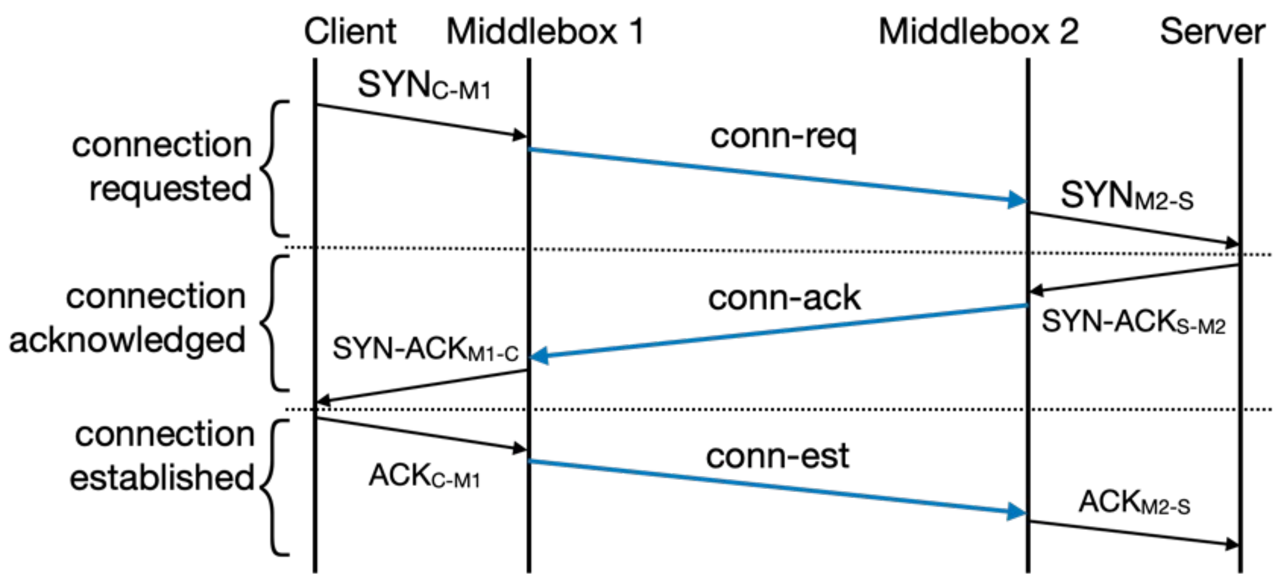
\includegraphics[width=\columnwidth]{figures/conn-est.pdf}
        %    \label{fig:connection}
        %    }
    %%\end{figure}
    %%\begin{figure}[t]
    %%    \centering
    %    \subfigure[Time line of connection termination in {\sys}] {
        %%    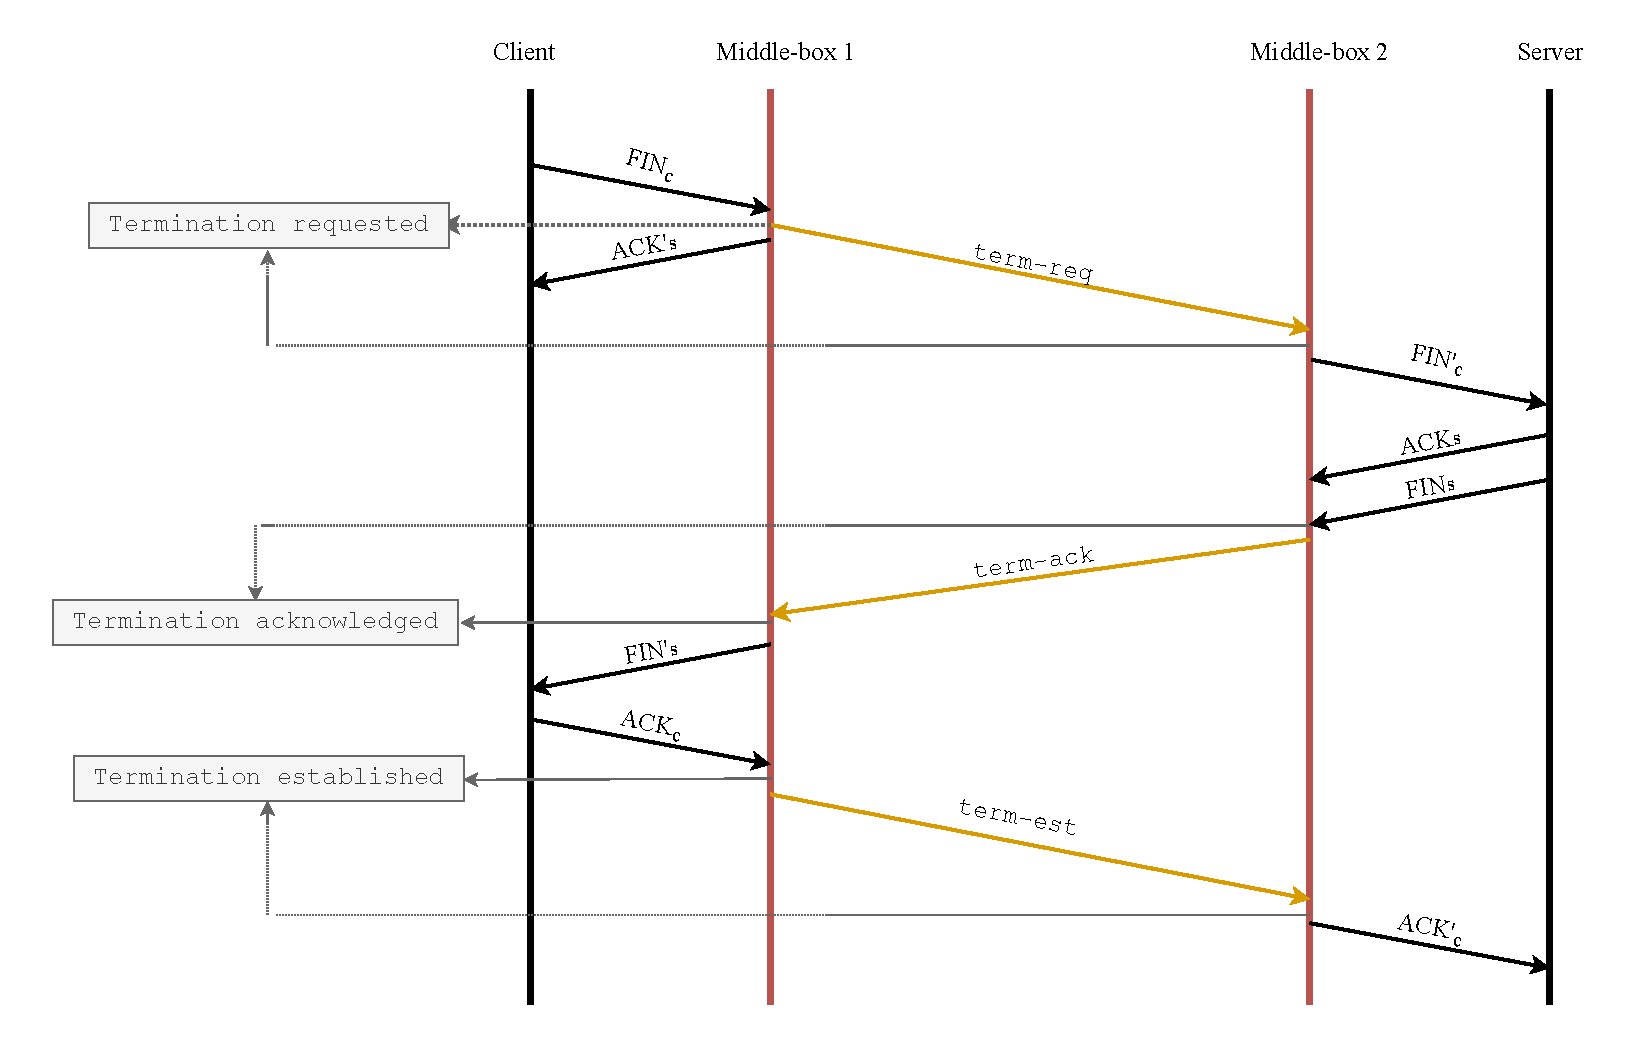
\includegraphics[width=\columnwidth]{figures/connection_termination.pdf}
        %    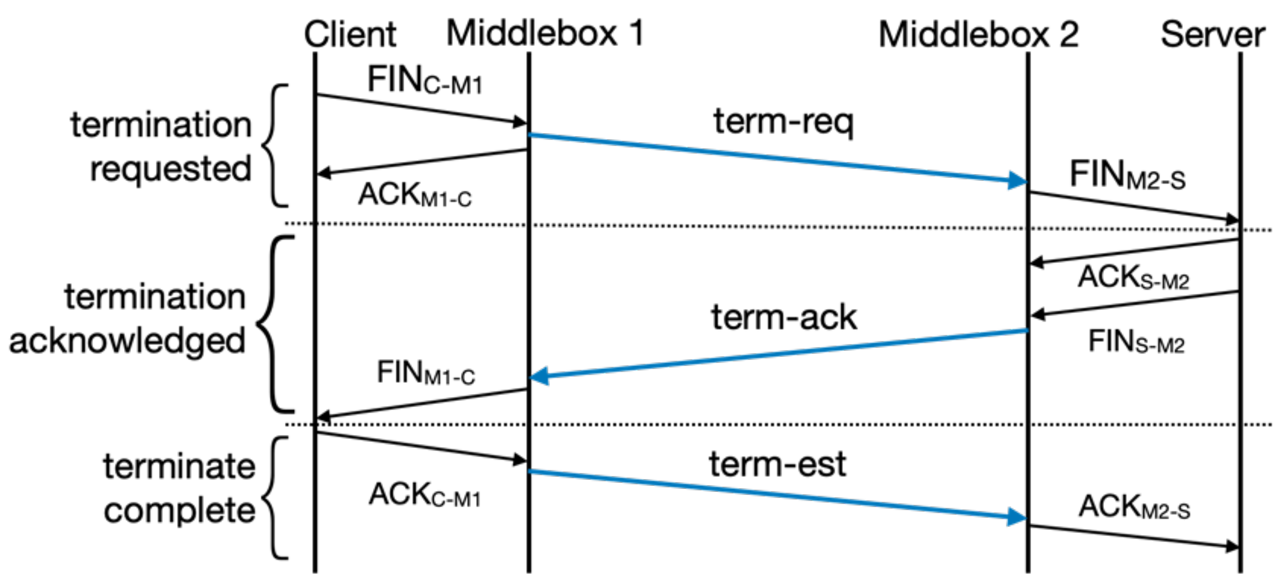
\includegraphics[width=\columnwidth]{figures/conn-term.pdf}
        %    \label{fig:termination}
        %    }
    %}
%\caption{Foo}
%\end{figure*}
%

\subsection{{Security Analysis}}
\label{subsec:impl-security}
{\sys} provides the following security property: an adversary cannot infer
application secrets from observing tunnel traffic. This
property is ensured by a combination of a secure shaping strategy, the tunnel design,
and implementation.

{\bf S1. Secure shaping strategy.} The tunnel transmits traffic in
differentially private-sized bursts
in fixed intervals. Thus, the overall shape is DP. The proof of DP is in
\S\ref{appendix:dp}.

{\bf S2. Secure tunnel design.}
(i) The privacy guarantees of a tunnel are configured before the start of
application transmission and do not change during the tunnel's lifetime.
(ii)~The tunnel mediates control between the end hosts, \eg by
transmitting custom connection establishment and termination messages. These
messages are subject to the same DP shaping as the payload traffic
(\S\ref{subsec:design-overview}).
%(iii)~All payload traffic of a sensitive application passes through a tunnel
%between a pair of middleboxes and is subjected to DP shaping and encryption.
(iii) The payload and dummy bytes in network packets are indistinguishable
because all payload and dummy bytes are packaged into QUIC packets and
encrypted uniformly. Moreover, QUIC handles acknowledgements, congestion
control, and loss recovery for both payload and dummy bytes uniformly
(\S\ref{subsec:design-overview}).

{\bf S3. Secure middlebox implementation.}
{(i)} The unshaped traffic between an end host and its local middlebox is
not visible to an adversary.
(ii) {\dshaper} follows the tunnel design in transmitting payload and dummy
bytes.
%
%(i) The control traffic between end hosts is intercepted at the middleboxes and
%is not directly sent into the tunnel.
%
%(ii) The payload and dummy bytes in network packets are indistinguishable. This
%is because both payload and dummy bytes are packaged into QUIC packets and
%encrypted uniformly. Thus, QUIC handles acknowledgements, congestion control,
%and loss recovery for both payload and dummy bytes
%(\S\ref{subsec:impl-shaping}).
%(iii) The sizes and timing of transmitted packets are secret-independent,
%because
(iii) The time required for {\prepare} to prepare and enqueue shaped
buffers is masked to secret-independent times. The packetization of~buffers in
QUIC is secret-independent~(\S\ref{sec:implementation}) and
%(\S\ref{subsec:impl-shaping-security}) and
thus retains DP guarantees after post-processing.
Any delays in transmitting the buffers can arise only due to congestion or
packet losses in the tunnel network, which are secret-independent events.
%(iii) The time required to {\em prepare} the DP-sized buffers is independent of
%application secrets. This is because {\sys}'s periodic interval is configured
%such that it can handle all DP sizes. Thus, any delays in transmitting the
%buffers can only arise due to congestion or packet losses in the tunnel network,
%which are secret-independent events.
%\todo{(iv) TODO: Verify that the middleboxes' handling of flow control do
%not reveal secrets.}
%
%
%{\bf S6.} No leaks are possible via the traffic shape of a non-sensitive
%application, which is physically isolated (by assumption in our threat model).

%\am{Discuss how middlebox's acks, handling of cc, flow control, loss recovery do
%not reveal secrets.}

%\subsection{Mitigating side-channel leaks}
%\label{subsec:impl-side-channels}
%A key challenge in ensuring sound {\nsca} mitigation could be side channels that
%may impact the middlebox execution and reveal secrets. We first list the
%sensitive information that can be potentially leaked via side channels and then
%discuss mitigations for the leaks.
%
%%\paragraph{Secrets.}
%There are three main types of secrets: the application data, the session keys
%for E2E encryption on the end hosts, and the session keys for tunnel encryption
%in the middlebox. Deviations of the tunnel transmissions from the DP schedule
%could be correlated with these secrets, thus revealing the secrets to a network
%observer.
%%%
%Since a middlebox is physically isolated from the end hosts, application keys
%and data cannot directly influence the middlebox execution. However, the
%application secrets could manifest into its traffic shape through its flow
%control mechanism. We elaborate this with two scenarios.
%%Thus, we only need to {\em performance isolate} the middlebox
%%execution from the application's flow control and from the tunnel's keys.
%
%\emph{Application flow control.}
%Consider an end-host application transmitting two secrets files A and B, each of
%length $L_A$ and $L_B$ bytes, respectively, with $L_A < L_B$. Suppose that the
%application transmits $L_A$ bytes to the middlebox in time $T_A < T$, whereas it
%transmits $L_B$ bytes in time $T_B$ that spans two intervals of duration $T$,
%say $L_{B_1}$ and $L_{B_2}$ in each interval, such that $L_{B_1} + L_{B_2} =
%L_B$.
%%Consider two consecutive intervals at the middlebox $T_i$ and $T_{i+1}$ and
%For simplicity, suppose that the {\DPlogic} suggests transmitting $X$ bytes in
%each shaping interval, where $X > max(L_A,~L_{B_1},~L_{B_2})$.
%Now, suppose the application transmits files A and B consecutively, with file A
%being transmitted just before the interval $T_i$ and file B being transmitted
%just before the interval $T_{i+2}$ at the
%middlebox. The {\DPlogic} will prepare buffers for transmission in each interval
%as follows: $T_i: [L_A,~X - L_A],~T_{i+1}: [0,~X],~T_{i+2}: [L_{B_1},~X -
%L_{B_1}],~T_{i+3}: [L_{B_2},~X - L_{B_2}]$.
%%The first buffer will contain $L_A$ bytes of A and $X - L_A$ dummy
%%bytes, while the second buffer will entirely contains $X$ dummy bytes.
%First, processing payload and dummy bytes could take different amounts of time.
%For
%instance, adding dummy bytes could consistently take a few microseconds longer
%than copying payload bytes.
%Secondly, the execution of the {\DPlogic} could be influenced by the presence or
%absence of payload traffic from the application. For instance, in a shaping
%interval, the {\DPlogic} could be delayed or interrupted if the application
%sends traffic and otherwise not. Such variances in the execution of {\DPlogic}
%could ultimately manifest into observable timing of the buffer transmissions in
%the tunnel, which could reveal information about the buffer contents (\eg
%whether they contain dummy bytes or not).
%
%\emph{DShaper secret keys.}
%The final secret in the tunnel are the keys used to encrypt the shaped traffic
%in each tunnel session. Prior work has shown how crypto keys can be leaked via
%various timing and microarchitectural side channels. Leak of the session keys
%would allow a network observer to decrypt all tunnel traffic, thus invalidating
%packet padding mitigations.
%
%Thus, we need to {\em performance isolate} the middlebox execution from the
%application's flow control and from the tunnel's keys.
%
%\paragraph{Mitigation.}
%For performance isolation, we rely on a combination of resource partitioning,
%performance masking, and \todo{constant-time implementation} techniques.
%First, we isolate the host-facing network stack and the tunnel stack into
%separate VMs, which run on separate cores and have dedicated access to separate
%physical NICs, DRAM and cache partitions. Furthermore, the interrupts for each
%VM are dedicated to the respective cores.
%
%Next, the execution of the {\shapedVM} could be affected by the memory partition
%hosting the datastructures shared with the {\unshapedVM} as well as the tunnel's
%keys which are used for encrypting the shaped packet.  To address this, we pin
%the datastructures in cache and implement the {\DPlogic} in constant time, and
%we assume that the crypto implementation is constant time as well.
%Finally, we {\em mask} the variance in the execution time of the path from the
%{\DPlogic} to the \todo{tunnel's network stack}. For this, we profile the
%worst-case execution time of this path and we delay forwarding of each packet
%to the
%stack until this worst-case time. Note this masking technique is conceptually
%similar to that proposed in Pacer~\cite{mehta2022pacer}. \am{refine the
%description}
%
%With the above mitigations in place, the only remaining side channels are due to
%the resources that fundamentally remain shared -- the internal buses and the
%off-core units that are shared among all cores (\eg APIC).  \todo{{\sys} does
%    not explicitly address side channel leaks via these resources.} \am{Check
%    DAGuise to justify this.}

\subsection{Deployment and Maintenance}
\label{subsec:design-discussion}
{\sys}'s tunnel endpoint design and implementation are both very modular and
portable.
The middlebox components are compatible with all application layer protocols
(\eg HTTPS, QUIC-TLS) and network stacks (\eg TCP, UDP, QUIC stacks).
The {\ushaper} could also be implemented as a standard SOCKS5 proxy~\cite{torpt}.
%The {\ushaper} component is compatible with all application layer protocols,
%such as HTTPS and QUIC-TLS. It could also be implemented as a standard SOCKS5
%proxy~\cite{torpt}. Similarly, the {\dshaper} is compatible with all transport
%protocols and network stacks.

A tunnel endpoint could be integrated with any node along an application's
network path as long as the application traffic is unobservable until egress
from the tunnel.
%
By integrating with a trusted VPN gateway of an organization,
network administrators could manage ``long-term'' tunnels between the
organization's campuses and support multiple applications without modifying
individual end hosts. For instance, separate tunnels may be configured
per-application according to the organizational needs, or
configurations may be adapted based on coarse-grained changes in the traffic
patterns through the~day.

Alternatively, by integrating with end user devices, \eg with VPN clients,
users could instantiate a new bidirectional tunnel with a service before
each network activity, choose a different configuration for each tunnel
instance, and close the tunnel after completion of the activity. A key
requirement would be to secure the tunnel endpoint's execution from any internal
side channels on the end host, which would be now more prevalent than in the
middlebox setup.


\section{Evaluation}
\label{sec:eval}

%\paragraph{Evaluation overview.}
Our evaluation answers the following questions.
(i) How well does {\sys} mitigate state-of-the-art network side-channel attacks?
%\mis{I woud be inclined to start with this.}
{(ii) What are the overheads associated with varying DP relevant
configuration parameters?}
%(ii) What are the theoretical bounds of differential privacy guara2.5 and the
%associated overheads in network side-channel mitigation?
(iii) What are the packet latency overheads and the peak line rate and
throughput sustained by our {\sys} middlebox?
(iv) What are {\sys}'s overall costs on privacy, bandwidth, client latency, and
server throughput for different classes of applications?
(v) How do {\sys}'s privacy guarantees and performance overheads compare to
prior techniques?

\if 0
(i) What are the trade-offs in the choice of various configuration parameters
that affect packet latencies, bandwidth overheads, and privacy guarantees?
(\Cref{subsec:privacy-microbenchmarks}
(ii) What are the optimal packet latencies, line rate, and number of concurrent
tunnels that can be supported by a MinesVPN middlebox?
(\Cref{subsec:perf-microbenchmarks})
(iii) Does MinesVPN mitigate network side-channel attacks in the applications?
(\Cref{subsec:attack-eval})
(iv) What are privacy guarantees, and the overheads on bandwidth, client latency
and server throughput due to {\sys}'s shaping on different classes of
applications---video and web?  (\Cref{subsec:eval-video,subsec:eval-web})
(v) How do {\sys}'s privacy guarantees and performance overheads compare to
prior techniques? (\Cref{subsec:eval-video,subsec:eval-web})
\fi
%(iii) What are the trade-offs between privacy guarantees and bandwidth overheads
%incurred for the applications?
%(v) What are the overheads on client response latencies and peak server
%throughput of the applications using MinesVPN?
%In the following subsections, we present (i) an empirical evaluation of the
%trade-offs between privacy leakage rate and the overheads incurred due to
%{\sys}'s differentially private shaping, (ii) microbenchmarks to analyze the
%overheads introduced due to {\sys}'s middleboxes, (iii) {\sys}'s impact on
%client latencies and server throughput in the context of our two applications,
%and (iv) an empirical evaluation of {\sys}'s security in the two applications.

%{\sys}'s middlebox components can run on top of a standard Linux kernel.
For our experiments, we use four AMD Ryzen 7 7700X desktops each with eight 4.5
GHz CPUs, 32 GB RAM, 1 TB storage, and one Marvell AQC113CS-B1-C 10Gbps NIC. We
simulate client and server applications on two of the desktops and {\sys}'s
middleboxes on the other two desktops.
The middleboxes are connected to each other via an additional Intel X550-T2
10Gbps NIC on each desktop.
%The middleboxes contain one additional Intel X550-T2 10Gbps NIC each and are
%connected to each other via these NICs.
The client and server desktops are connected to one of the two
middleboxes each via the Marvell NICs, overall forming a linear topology.

We implemented the {\ushaper} and {\dshaper} processes in
\update{1100} and \update{1800} lines of C++ code, respectively, and deployed
them on Ubuntu OS 22.04.02 (kernel version 5.19).
{\sys} relies on the MSQUIC implementation of QUIC, libmsquic v2.1.8, which
includes OpenSSL for traffic encryption, contributing an additional
\update{180713} LoC to {\sys}'s TCB.

For rapid evaluation, we  built a simulator,
which implements the {\prepare} thread's DP logic.
The simulator transforms  an application's original packet sequence (from
tcpdump) into a sequence of burst sizes within fixed-length
intervals, and outputs a sequence of transmit sizes corresponding to DP
queries.
%
{We confirmed that the bandwidth overheads from the simulator closely match
the overheads observed on the testbed. Thus, we report privacy and
bandwidth overhead results from the simulator and latency and
throughput results from the testbed, unless specified otherwise.}
%We implement {\sys}'s middlebox on a \todo{X} server with \todo{8} \todo{Intel
%XXX} CPUs, \todo{X} RAM, and \todo{two Intel XXX XGbps} NICs. We disable
%hyperthreading and dynamic voltage and frequency scaling (DVFS) on the servers
%mainly to reduce variance in the empirical measurements. We use two KVM virtual
%machines to host the network stacks of {\unshapedVM} and {\shapedVM}.  Each VM
%is configured with \todo{X vCPUs, X GB RAM and X GB storage} and is connected
%to one NIC each. Each VM's vCPUs are statically pinned to one physical core
%each. The VMs run on \todo{Ubunutu XXX and XXX kernel}. The {\shapedVM} runs
%the \todo{QUIC version XXX}~\cite{QUIC} on top of the kernel.
%

%In principle, {\sys} can support arbitrary protocol stacks on the end hosts.
%In our evaluation, we consider applications using TCP, which presents the most
%challenging protocol stack due to its own implementation of reliable delivery,
%congestion control, flow control, loss recovery, and retransmissions.
We use two applications for case studies, a video streaming service and a
medical web service, which we describe below. Both applications are hosted on an
Nginx 1.23.4 web server and the datasets are stored on the host file system.
%We evaluate {\sys}'s effectiveness in hiding from an adversary the time and
%content of clients' interactions with these services, and the bandwidth,
%latency, and throughput overheads incurred due to shaping.
%We briefly describe the services below.

\textbf{Video service.}
The video streaming service is used to serve \update{100 YouTube videos} in 720p
resolution with \update{5 min to 130.3 min (median 12.6 min)} durations and
\update{2.7 MB to 1.4 GB (median 73.7 MB)} sizes.
We implement a custom video streaming client in Python, which
uses one TCP connection for a single stream and requests individual 5s segments
from the service synchronously.
Unless specified otherwise, we stream the first 5 min of videos in our
experiments. The configuration is in line with that used in prior
work~\cite{schuster2017beautyburst} and reasonable, given the popularity of
short videos~\cite{videostats}.
%to fetch all segments of a single video~stream.

%We implemented a custom video streaming service in PHP, which is hosted using
%Apache HTTP Server \todo{XXX}, and returns video segments in response to client
%requests. We host \todo{1218} Youtube videos in 240p and 720p bitrates, which
%are generated using MPEG-DASH encoding. The videos have durations
%ranging from \todo{X min to 4.2 hours (median: 7 min)}, and with the
%video sizes ranging from \todo{X KB to 6.2 MB (median: 6.2 MB)}. \todo{TODO:
%comment on simulating a live streaming setup.}
%%
%We also implemented a custom client in Python, which first requests
%for the MPD segment of a video from the server, parses the MPD, and then
%requests for subsequent video segments sequentially.

\if 0
\paragraph{VoIP.}
\am{May go depending on the results. Replace with multi-tier web service
instead.}
We use FlexiSIP~\cite{flexisip} as a VoIP server and
Linphone~\cite{linphone} application as a client, both of which are hosted in
separate containers on Docker \todo{XXX version} inside a VM with \todo{Ubuntu
18.04 LTS and XXX kernel}. We use the DAPS dataset~\cite{daps} of \todo{X}
audio clips from \todo{source}~\cite{audio-dataset}. The audio clips are
encoded using \todo{G.722} and have durations ranging from \todo{X-Y min
(median: Z min)} and sizes ranging from \todo{X-Y KB (median: Z KB)}.
\fi

\textbf{Web service.}
The web service is used to serve a corpus of {96} static HTML pages of a medical
website, whose sizes range from \update{54 KB to 147 KB (median: 90 KB)}.
{As a client, we use modified wrk2 \cite{wrk2} that issues concurrent
asynchronous HTTPS GET requests at a specified rate.}

For all experiments, we use one baseline setup and one of three {\sys}
configurations.
In the baseline setup ({\base}), the client is directly connected to the server.
In the simulator setup ({\nssim}), we generated sequences of shaped burst sizes
using DP shaping.
With {\sys}, the traffic between the client and the server passes through two
middleboxes, each implementing {\ushaper} and {\dshaper}.
We consider two configurations of the middleboxes:
(i) {\nsnoshape}: {\dshaper} does not implement shaping (\ie neither DP noise
sampling nor the fixed length loop interval $\dpintvl_{max}$), allowing us to
measure the system overheads due to the middlebox implementation, and
(ii) {\ns}: {\dshaper} implements the full shaping mechanism.
{By default, each middlebox is configured with 128 pairs of per-flow
transmit and receive queues (unless specified otherwise). We configure the queue
sizes for the max data that can be transmitted at line rate for a given
DP shaping~interval. We configure a max cutoff for the shaped buffer length
based on the max burst length of the application and the number of active
flows. This implies that the number of flows is public.}
%each of length 12.5 MB (unless specified otherwise).}
% \ml{This mean that the total number of flow is public in \sys.}
% \ml{Point to the fix if we have it!}

In addition, we compare with two other shaping strategies: constant-rate shaping
({\constshape}), which is the most secure shaping strategy, and Pacer
({\pacer}), a SOTA system that shapes traffic on a per-request basis.
%We compare bandwidth overhead of {\sys} with the overheads~that would be
%incurred due to constant rate shaping ({\constshape}) and~Pacer
%\cite{mehta2022pacer} (\S\ref{subsec:eval-comparison}), a SOTA system that
%provides dynamic shaping on a per-client request basis.
%We also compare the accuracy of attacks on traffic shaped by {\sys}, constant
%rate shaping and Pacer (\S\ref{subsec:attack-eval}).
For {\constshape}, we configure the peak load corresponding to the largest
object sizes in our applications, which involves transmitting 1.7MB in 5s for
videos and 57KB in 50ms for web.
For Pacer, we pad all web pages to the largest page size, \ie 147KB in our
dataset. For videos, Pacer pads a segment at $i$\textsuperscript{th} index
in a video stream to the largest segment size at that index across all videos in
the dataset.


\begin{figure}[t]
    \centering
    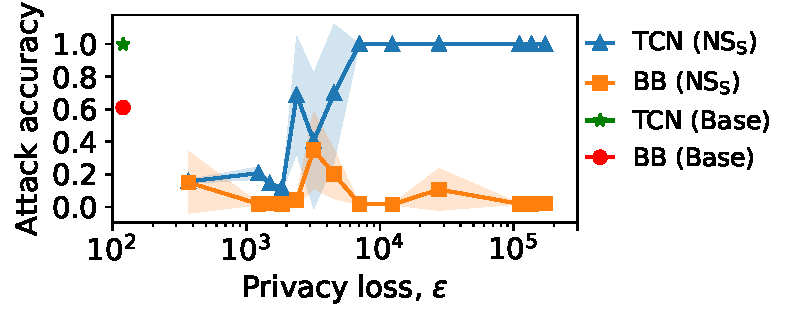
\includegraphics[width=0.85\columnwidth]{accuracy_vs_privacy_loss_video_updated.pdf}
    \caption{\update{Classifier accuracy on shaped traces.}
        %    \am{Change label from {\ns} to {\nssim}}
    }
    %\am{How is the blue shaded area going higher than accuracy of 1.0?}\as{The
        %blue shaded area is +-std so it can be larger than one or smaller than
        %zero.}
    \vspace{-0.4cm}
    \label{fig:empirical-privacy}
\end{figure}

\subsection{{\sys} Defeats Attack Classifiers}
\label{subsec:attack-eval}
%\todo{We need to explain that the accuracy of classifier on pacer and CR is as
%good as random guess (\ie 2.5\%)}.
%\\
%\am{Allude to formal proof of guarantees and security by design.}
%We measure the impact of the privacy configurations on the performance of
%attack classifiers \todo{from \S\ref{subsec:attack-bg}} on shaped traffic of
%video streams.
We start with an empirical evaluation of the privacy offered by {\sys}'s traffic
shaping. Recall that the traffic shaping depends on several DP parameters: the
window length $\winlen$, the sensitivity $\qsens$, the length of the DP
interval $\dpintvl$, and the privacy loss $\varepsilon$.
%We train the classifiers from
%\S\ref{subsec:attack-bg} on shaped video traffic generated with varying
%$\epsilon_w$ values and evaluate their accuracy.
%Furthermore, we identify the weakest privacy configuration that is able to
%successfully defeat the classifiers.
We evaluated the classifiers from \S\ref{subsec:attack-bg} on shaped traffic generated using various values of these DP relevant parameters.
We present the classifiers' performance based on~only one set of values for
$\winlen$, $\qsens$, and $\dpintvl$, while varying $\varepsilon$ between
\update{[200, 200000]}.
Our goal is to provide intuition about what values of $\varepsilon$ are
sufficient to thwart a side-channel~attack.
%We analyze the performance of the classifiers on network
%traces collected from the testbed in our local network.
%\todo{We collect tcpdump traces from the {\dshaper} process in both the
%middleboxes and apply the TCN and BB classifiers on the collected traces.
%Note that these traces present a best case for the adversary;
%in practice,
%%under the assumption that the adversary is not colocated with the application,
%(i) the adversary can only measure the traffic between the middleboxes, and (ii)
%real measurements likely have more noise due to interference from other traffic
%on the Internet.}

We set (i) $\winlen = 5s$ to align with the 5s video segments that comprise the
videos, (ii) \update{$\qsens = 2.5 MB$}, \update{which covers 99th \%ile}
of the distances in our dataset (\S\ref{sec:eval-extended}), and
(iii) $\dpintvl = 1s$, which
leads to composing the privacy loss over $\varnumupdates = 5$ DP queries on
the buffering queues. The 1s interval provides a reasonable trade-off between
privacy loss, and bandwidth and latency overheads, which we
discuss in the subsequent sections.
%We discuss the rationale behind the configuration choices in the subsequent
%sections.
%
%We~vary per-window privacy loss, $\varepsilon_\winlen$, between \update{[100,
%10000]}.

We used 40 videos of 5 min duration each. We streamed each video 100 times
through our testbed without shaping~and collected the resulting tcpdump
traces. For each value of \update{$\varepsilon$}, we transformed each unshaped
trace into a shaped trace using our simulator to generate a total of 4000
shaped traces.
%For {\constshape} we pad each video segment to 1.7 MB and transmit it in
%5s intervals. For Pacer, we group all videos into a single cluster and pad the
%$i$\textsuperscript{th} segment in each video to the largest segment size at
%that index across all videos in the dataset.
We also shaped traces for {\constshape} and {\pacer}.
%We then train the classifiers on the shaped traces using 80-20 train-test split,
%similar to \S\ref{subsec:attack-bg}.


%For shaping, we set $\ssens = 1MB$, $\winlen = 5s$, and perform DP
%queries at $\dpintvl = 1s$ intervals in each window.
%\mis{Why???}
%For shaping, we select (i) window length ($\winlen$) of 5s, because it aligns
%with the 5s video segments that make up the videos, (ii) sensitivity ($\ssens$)
%of 1 MB, which covers 97\% of the video streams in our dataset
%(\S\ref{sec:eval-extended}), and (iii) interval length ($\dpintvl$) of 1s,
%which
%leads to composing privacy loss over 5 DP queries of the buffering queues
%(i.e. $\varnumupdates = 5$).
%We~vary per-window privacy loss, $\varepsilon_\winlen$, between \update{[100,
%10000]} and, for each value of $\varepsilon_\winlen$, we collect \update{100}
%normalized traces each of the shaped traffic of \update{40} videos streamed for
%\update{5 min}.
%Classifier training is same as in \S\ref{subsec:attack-bg}.


\update{
We train and test BB and TCN on shaped traces as in \S\ref{subsec:attack-bg} and
report the average and standard deviation of the accuracy of each classifier
over three runs.
}
Recall from \S\ref{subsec:attack-bg}, the BB and TCN accuracy on unshaped
traffic ({\base}) is 0.61 and 0.99, respectively.
%generated using the above configurations.
%\mis{I think this would be more helpful if we could draw lines at the accuracy
%of each model on unshaped, but encrypted traffic. I found the explanation below
%confusing, but didn't want to try to rewrite it without seeing how well the
%models do on the encrypted but unshaped traffic. In my mind, the high level take
%away is that $epsilon_W$ of between $10^2$ and $10^3$ is sufficient to thwart a
%state of the art attack; given that, the results from the current 6.1 can now be
%put in context, because we can explain how much that costs in terms of
%overhead.}
\update{For {\constshape} and {\pacer}, the accuracy of both BB and TCN
classifiers is 0.025. This is expected since both strategies transform all
unshaped traces into a single shape.
}

\Cref{fig:empirical-privacy} shows the classifiers' performance with {\sys}.
%(markers show average, shaded region shows the standard deviation).
While BB does not perform well for nearly all values of \update{$\varepsilon$},
TCN can be thwarted for \update{$\varepsilon$} upto 1000.
%
%We should
%\todo{We get similar results even when generating shaped streams with $\dpintvl
%= 0.1s$.}
{\em While even \update{{$\varepsilon \approx 200$}} is too
large to offer meaningful theoretical privacy guarantees, it is sufficient to
defeat SOTA attacks.}
%\mis{This seems like a really important result or observation; I believe
%what we're saying here is that theoretical analsys suggests that you need
%quite strong privacy guarantees, but from a practical perspective, this
%applicaiton requires much weaker guarantees.  I think this has potentially
%significant consequences.}
%\Cref{subfig:high-sensitivity-epsilon-sigma} shows that $\varepsilon_{\winlen} =
%100$ yields a noise overhead of $< 1 MB$ per window.

%While BB does not perform well for nearly all values of $\varepsilon_{\winlen}$,
%TCN's accuracy is less than 0.2 and close to 1.0 for $\varepsilon_{\winlen} =
%100$ and $\varepsilon_{\winlen} > 1000$, respectively.
%and \Cref{tab:attack_performance} demonstrates the performance of the same
%classifiers on the unshaped traffic.
%
%From \Cref{subfig:high-sensitivity-epsilon-sensitivity}, $\varepsilon_{\winlen}
%= 100$ yields a noise overhead of $< 400KB$ per window.
%The results highlight {\em (i) the huge gap between the theoretical DP
%guarantees and the configurations required to defeat SOTA attacks, and (ii)
%the costs of privacy required in the face of more sophisticated attacks in the
%future.}

\begin{figure}[t]
    \centering
    \begin{subfigure}{0.49\columnwidth}
        \centering
        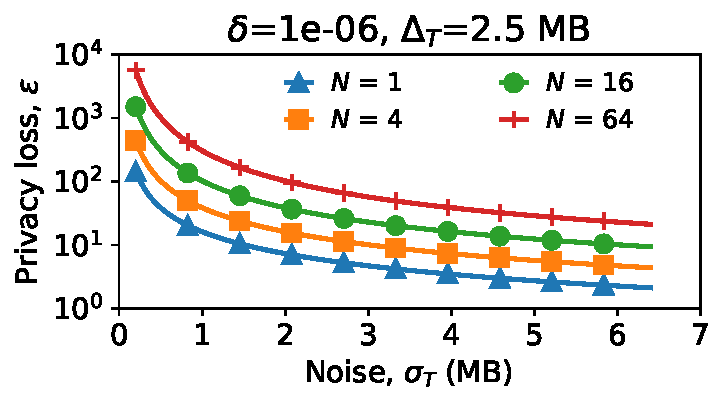
\includegraphics[width=\textwidth]{privacy_loss_VS_noise_std_video_updated.pdf}
        \caption{}
        %        \caption{Noise vs privacy loss}
        \label{subfig:high-sensitivity-epsilon-sigma}
    \end{subfigure}
    \hfill
%    \begin{subfigure}{0.33\textwidth}
    %        \centering
    %
    %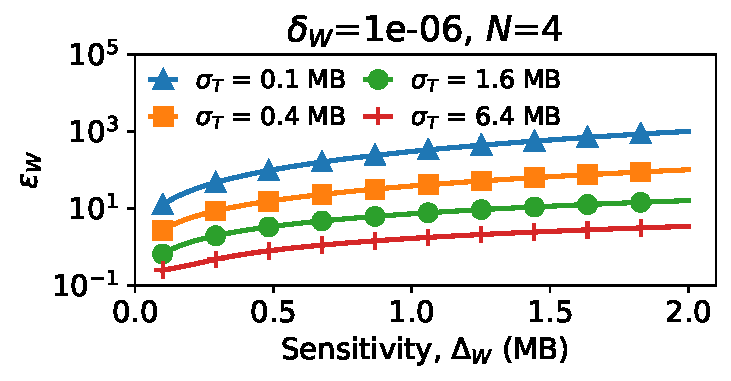
\includegraphics[width=\textwidth]{plots/privacy_loss_VS_sensitivity_video.pdf}
    %        \caption{Sensitivity vs privacy loss}
    %        \label{subfig:high-sensitivity-epsilon-sensitivity}
    %    \end{subfigure}
%    \hfill
    \begin{subfigure}{0.49\columnwidth}
        \centering
        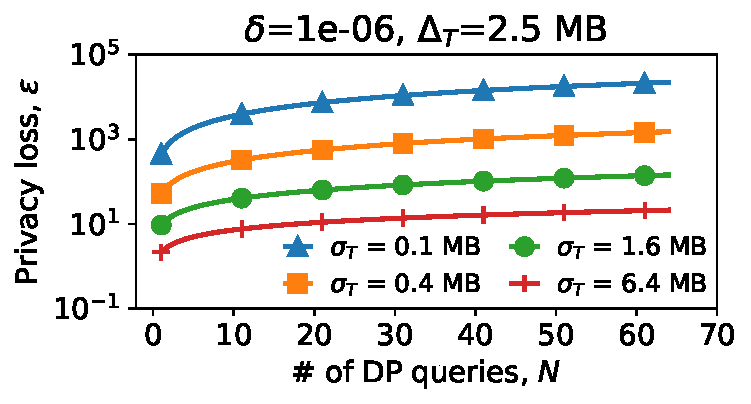
\includegraphics[width=\textwidth]{privacy_loss_VS_query_num_video_updated.pdf}
        \caption{}
%        \caption{\# of DP queries vs privacy loss}
        \label{subfig:high-sensitivity-epsilon-queries}
    \end{subfigure}
    \caption{
      \update{Privacy loss vs
      (a) noise and (b) \# of DP queries.}
%    \am{Make notations consistent.}
    }
    \vspace{-0.4cm}
    \label{fig:privacy-microbenchmarks}
\end{figure}


% \subsection{Theoretical Privacy Analysis}
\subsection{Impact of Privacy Parameters}
\label{subsec:privacy-microbenchmarks}

%We start by comparing the relation between DP relevant configuration parameters.
%Recall from \S\ref{sec:dp}, {\sys}'s privacy loss ($\varepsilon_\winlen$) and
%bandwidth overheads due to DP noise (represented by $\sigma_\dpintvl$, \ie the
%standard deviation of the noise distribution function) depend on:
%Recall from \S\ref{sec:dp} that {\sys} shapes traffic in uniform intervals of
%length $\dpintvl$, defined within a larger window of $\winlen$. Thus, {\sys}'s
%bandwidth overheads due to DP noise (denoted by $\sigma_\dpintvl$, \ie the
%standard deviation of the noise distribution) is measured in $\dpintvl$, while
%privacy loss ($\varepsilon_{\winlen}$) is defined in $\winlen$. These metrics
%depend on $\ssens$, $\delta_{\winlen}$, $\winlen$, and
%$\varnumupdates = \numupdates$.
%%Rather than exploring different values of $\winlen$ and $\dpintvl$, we
%%analyze $\varepsilon_{\winlen}$ and $\sigma_\winlen$ costs as a factor of
%%$\varnumupdates$.
%Given values for $\ssens$ and $\varnumupdates$, the
%$\varepsilon_{\winlen}$ and $\sigma_\dpintvl$ costs remain the same at
%different time scales.
%Thus, we explore $\varepsilon_{\winlen}$ and $\sigma_\dpintvl$ costs for
%different ranges of $\ssens$ and $\varnumupdates$, and analyze the impact of
%$\winlen$ and $\dpintvl$ on latency overheads separately.
%\ml{I don't get what these last few sentences mean? Is something like ``The
%core parameters influencing the behavior of the system are $\varnumupdates$
%and
%$\sigma_\dpintvl$. We thus explore their impact of the DP guarantee
%$\varepsilon_{\winlen}$. We analyse the impact of $\winlen$ and $\dpintvl$ on
%latency overheads separately.''?}
%A value of $x$ for $\varepsilon_\winlen$ implies that the probability of
%identifying the traffic content given a shape is $e^{x}$.
%The value of $\sigma_\winlen$ indicates the standard deviation of the noise
%distribution function, which estimates the amount of overhead that would be
%added to the original traffic due to DP shaping.
%All analyses use $\delta_\winlen = 10^{-6}$.
%which is a typical value in DP mechanisms.
%\mis{This could use a reference.}
%\ml{we could stick to ``All analyses use $\delta_\winlen = 10^{-6}$.'', it's a
%longer discussion and I don't know good citations...}
%At a high level, $\winlen$ affects $\ssens$, while $\ssens$,
%$\varepsilon_\winlen$, $\delta_{\winlen}$, and $\varnumupdates$

We now  evaluate how $\varepsilon$ varies with $\qsens$,
$\sigma_\dpintvl$, and $\varnumupdates$.
Due to space constraints, we present plots for a fixed value of $\qsens
= 2.5 MB$ and defer other plots to \S\ref{sec:eval-extended}.
All analyses use $\delta = 10^{-6}$.

\Cref{subfig:high-sensitivity-epsilon-sigma} shows the tradeoff between
$\varepsilon$ and $\sigma_\dpintvl$ over four different values of
$\varnumupdates$.
Intuitively, a larger
$\sigma_\dpintvl$ implies higher bandwidth overhead due to DP shaping.
To retain a total privacy loss $\varepsilon = 1$ with at most 4 DP
queries, we need to add noise with $\sigma_\dpintvl = 18 MB$ for each DP
query. In contrast, $\varepsilon = 200$ with 4 DP
queries (approx. configuration that defeats the classifiers
in \S\ref{subsec:attack-eval}) only requires $\sigma_\dpintvl < 0.3 MB$.
%We discuss how to amortize bandwidth overheads using concurrent flows
%without increasing privacy loss in \S\ref{subsec:eval-video} and
%\S\ref{subsec:eval-web}.
%
\Cref{subfig:high-sensitivity-epsilon-queries} shows that the
total privacy loss escalates with an increase in the number of DP queries.
While fewer queries within a window (thus larger decision intervals) help to
lower the total privacy loss, the tradeoff is the higher latency overhead. We
discuss this tradeoff, as well as reduction in bandwidth overheads with
concurrent flows in \S\ref{subsec:eval-video} and \S\ref{subsec:eval-web}.
%In \Cref{subfig:high-sensitivity-epsilon-sigma}, we observe that when the
%difference in queue sizes is limited to 1 MB (i.e., $\ssens = 1$ MB), achieving
%low privacy loss with only 4 DP queries within a window requires the
%addition of Gaussian noise with a standard deviation of 6 MB to each
%query. This can potentially result in significant overheads.
%The privacy loss further increases with more number of DP queries as it is
%illustrated in \Cref{subfig:high-sensitivity-epsilon-queries}. It is important
%to note that also {\sys} can mitigate SOTA attacks small overhead
%(\S\ref{subsec:attack-eval}), to achieve strong differential privacy guarantees
%with minimal privacy loss, larger overheads are generally necessary.
%Later on, we explain how large overheads can be amortized through the
%parallelization of flows (\S\ref{subsec:eval-video}, \S\ref{subsec:eval-web}).

%\mis{Is this not really simply the data overhead?  I don't know that the term
%"noise overhead" makes sense.}
%Next, for a fixed number of DP queries ($\varnumupdates = 4$),
%\Cref{subfig:high-sensitivity-epsilon-sensitivity} shows the increase in privacy
%loss with increasing values of sensitivity when maintaining four different noise
%overhead levels. If there is a significant variation in the buffering queue
%sizes across different streams, more noise is required to preserve the same
%level of privacy loss in the shaping mechanism.
%Each DP query increases privacy loss for application streams.
% Secondly, \Cref{subfig:high-sensitivity-epsilon-queries} shows the total privacy
% loss with increasing number of DP queries for maintaining different
% \todo{data overhead} levels.
% \mis{I think this section could be much more valuable if instead of simply
%saying that each chart illustrates a trade-off, we give a qualitative
%explanation
%of what the graph shows.  For example, (A) shows that increasing the number of
%DP-queries increasese overhead, that privacy costs overhead [having the
%results from the attack scenario would be super useful -- how much privacy do
%we
%need to thwart the re-identification attack], and that sometimes that overhead
%can be quite large (I read that it can cost us 6X the data transmission to
%provide the best privacy level!) Also, please add (log scale) where approprite
%on axis labels.}
% In \Cref{subfig:high-sensitivity-epsilon-sigma}, we observe that when the
%difference in queue sizes is limited to 1 MB (i.e., $\ssens = 1$ MB), achieving
%low privacy loss with only 4 DP queries within a window requires the
%addition of Gaussian noise with a standard deviation of about 6 MB to each
%query. This results in significant overheads.
% The privacy loss further increases with more number of DP queries as it is
%illustrated in \Cref{subfig:high-sensitivity-epsilon-queries}.
% It is important to note that also SOTA attacks can be mitigated with small
%overhead (\S\ref{subsec:attack-eval}), to achieve strong differential privacy
%guarantees with minimal privacy loss, larger overheads are generally necessary.
% Later on, we will provide an explanation of how large overheads can be
%amortized through the parallelization of flows (\S\ref{subsec:eval-video},
%\S\ref{subsec:eval-web}).

\if 0
%The privacy loss of our shaping mechanism is determined by the standard
%deviation of the noise that we apply to update the noisy measurement of the
%queue sizes.
%\Cref{subfig:high-sensitivity-epsilon-sigma} and
%\Cref{subfig:low-sensitivity-epsilon-sigma} demonstrates how increasing the
%standard deviation of applied noise decreases privacy loss for different number
%of updates. Furthermore, to obtain the same level of privacy loss, applications
%with high sensitivity (i.e. high variations in queue sizes) require larger
%values of noise.
%Note that the privacy loss is not affected by the length of the observation
%window preceding the update of the noisy measurement of queue sizes, and its
%magnitude is solely determined by the frequency of updates.
Figures \ref{subfig:high-sensitivity-epsilon-sigma} and
\ref{subfig:low-sensitivity-epsilon-sigma} demonstrate the trade-off between
noise overhead and privacy loss composed over four different configurations of
total number of DP queries and for $\ssens$~of 10MB and 100KB, respectively.

For a fixed value of number of updates, figures
\ref{subfig:high-sensitivity-epsilon-sensitivity} and
\ref{subfig:low-sensitvity-epsilon-sensitivity} show the increase in privacy
loss with increasing values of sensitivity when maintaining four different noise
overhead levels.
%The privacy loss of {\sys} shaping mechanism is also affected by the sensitivity
%of queue size measurements.
%\Cref{subfig:high-sensitivity-epsilon-sensitivity} and
%\Cref{subfig:low-sensitvity-epsilon-sensitivity} display the privacy loss of the
%shaping mechanism for varying values of sensitivity.
If there is a significant variation in the buffering queue sizes across
different streams, more noise is required to preserve the same level of privacy
loss in the shaping mechanism.

Each DP query increases privacy loss for application streams. Figures
\ref{subfig:high-sensitivity-epsilon-queries} and
\ref{subfig:low-sensitivity-epsilon-queries} show the total privacy loss with
increasing number of queries for maintaining different noise overhead
levels.
%particular value for the variance of the noise.
Note that the privacy loss increases faster for larger values of sensitivity.
\fi

Using these plots, an application can choose suitable values of $\winlen$ and
\update{$\qsens$} to determine the tradeoff between \update{$\varepsilon$} and
$\sigma_{\dpintvl}$.
For our web application serving static HTML, we recommend $\winlen =
1s$, since web page downloads in our AWS setup (\S\ref{subsec:attack-bg})
finished within 1s, and \update{$\qsens = 60 KB$}, which covers all distances.
\S\ref{subsec:attack-eval} explained the choices for our video application.
\update{
Using \update{$\varepsilon$} and $\dpintvl$, we can further determine the
aggregate privacy loss over longer traffic streams using R\'enyi-DP composition.
For instance, with \update{$\varepsilon = 1$}, $\winlen = 5s$, and $\dpintvl =
1s$, the total privacy loss for a 5 min video, which generates 300 DP
queries at 1s intervals, is 8.92; the total loss for a 1 hr~video is 38.8.
}
We emphasize that {\em \update{$\qsens$ and $\varepsilon$} should be selected
using plots like \Cref{fig:privacy-microbenchmarks},
independently of the application's dataset.}

\if 0
Using these plots, an application can choose suitable values of
$\ssens$ and $\winlen$ to achieve the desired trade-off between
$\varepsilon_{\winlen}$ and $\delta_{\winlen}$.
%$\ssens$, $\varepsilon_{\winlen}$, $\winlen$, and $\varnumupdates$ based on its
For our video streaming application, for instance, we recommend configuring
$\winlen = 5s$, because it aligns with the 5s video segments that make up the
videos, and $\ssens = 1 MB$.
Looking at the distribution of the difference between every pair of video
segments in our dataset (\Cref{fig:sensitivity-comparison}), this covers 97\% of
the video streams in our dataset.
Similarly, for our web application serving static HTML, we configure $\winlen =
1s$, since web page downloads in our AWS setup (\S\ref{subsec:attack-bg})
finished within 1s, and $\ssens = 185 KB$, which covers 95\% of the web pages in
our dataset.
We emphasize that {\em $\ssens$ and $\varepsilon_\winlen$ should be selected
using trade-off plots similar to \Cref{fig:privacy-microbenchmarks} and
independently of the application's dataset.}
%\mis{What do we mean by "consider"?  Do we really mean, "We recommend
%configuring the application this way because ...?"}
\fi

\if 0
We use video streaming and web services as representative examples of network
applications with high and low sensitivities, respectively.
\Cref{fig:sensitivity-comparison} shows the difference between queue sizes measured in our
middlebox during the transmission of video and web traffic.
An ideal sensitivity value should be greater than the majority of potential
differences between queue sizes.
%\Cref{fig:sensitivity-comparison} illustrates a box-and-whisker plot
%representing the differences in queue sizes for video and web traffic passing
%through our middlebox.
The whiskers show the minimum and maximum queue sizes, the box
shows the first and third quartiles and the dashed line shows the median of the
queue sizes.
Although, the sensitivity should not be adjusted based on a particular dataset,
\Cref{fig:sensitivity-comparison} illustrates that approximately 97\% of video
traces in our dataset can be considered neighbors when using a sensitivity of 1
MB. Similarly, for the web dataset, a sensitivity of 185 KB covers more than 95\% of
web traces.
\fi

% Note that the parameters are independent of the length of observation window,
% implying that the privacy and overheads are similar when applying the same DP
% noise the same number of times but with different shaping intervals. For
% instance, the privacy and overheads over 1s in 100ms intervals are the same as
% those over 100ms in 10ms intervals.


\subsection{Performance Microbenchmarks}
\label{subsec:perf-microbenchmarks}
We now turn our attention to experiments to determine the overheads on
per-packet latencies and the peak line rate and throughput sustainable by a
{\sys} middlebox.

\if 0
\begin{table}[t]
\centering
\begin{tabular}{llll}
    \toprule
    \textbf{Request size} & {\base~(avg)} & {\nsnoshape~(avg)} & \textbf{\%
    overhead} \\
    \midrule
    1.46 KB & 29999.87 & 29342.54 & 2.19
    \\
    14.6 KB & 27400.33 & 25967.91 & 5.23
    \\
    146 KB & 8039.04 & 787 & 2.07
    \\
    1460 KB & 804.6 & 798.34 & 0.78
    \\
    \bottomrule
\end{tabular}
\caption{Peak throughput (requests/s) of {\base} vs {\nsnoshape} \am{Replace
with a plot showing \#clients vs xput and \#clients vs latency
    for just the smallest and largest file sizes.}}
\label{tab:xput-nomask}
\end{table}
\fi

\begin{figure}[t]
    \centering
    \begin{subfigure}{0.49\columnwidth}
    \centering
    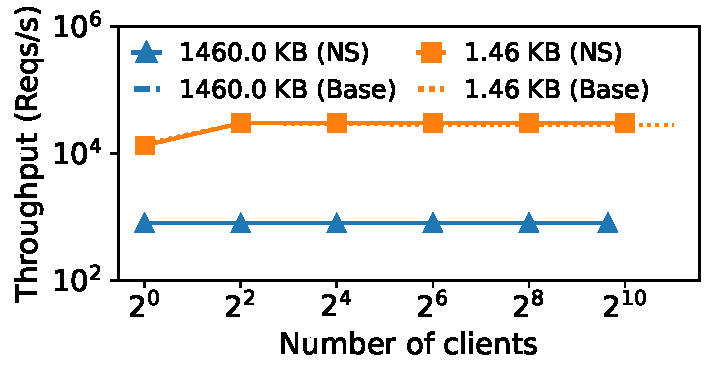
\includegraphics[width=\textwidth]{throughput_vs_client_num.pdf}
    \caption{\# clients vs throughput}
    \label{subfig:clients-vs-xput}
    \end{subfigure}
%    \hspace{30pt}
    \hfill
    \begin{subfigure}{0.49\columnwidth}
    \centering
    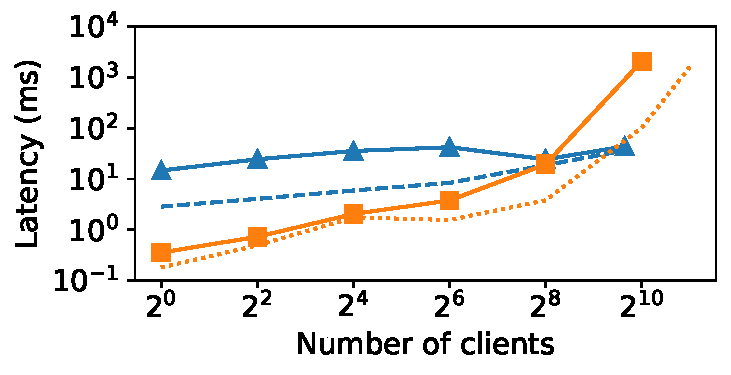
\includegraphics[width=\textwidth]{latencies_vs_client_num-logscale.pdf}
    \caption{\# clients vs latency}
    \label{subfig:clients-vs-latency}
    \end{subfigure}
    \caption{Throughput and latency overhead due to middleboxes without shaping.
%        \am{Show error bars.}
    }
    \vspace{-0.4cm}
    \label{fig:xput-latency-microbench}
\end{figure}

\textbf{Middlebox throughput.}
%We measure %the peak line rate,
%the peak throughput that can be sustained in a client-server system and the
%impact of concurrent clients on peak throughput and response latency.
\if 0
For line rate, we use iperf3 \citeme{iperf3} to generate a large number of
asynchronous requests from the client to the server and measure the peak load
sustained. \todo{We report the average line rate measured across three X min
runs of iperf3.} The {\base} sustains a line rate of \todo{9.4 Gbps} and, with
\todo{9.39 Gbps}, {\nsnoshape} can match the {\base} line rate. \am{Do we need
this?}
\fi
%
We measure the peak throughput (requests/s) attained by a server application,
the response latency experienced by the clients, and the impact on this
throughput and latency due to the middleboxes.
We restrict Nginx to one worker thread and one core on the server desktop.
We evaluate using two object sizes: 1.4 KB (one MTU) and 1.4 MB.
We identify the peak request rate that can be handled by a single wrk2 client,
then increase the clients until we find the peak throughput the server can
provide.
%Then, we vary the load by increasing the number of concurrent clients while
%fixing each client to generate the peak per-client request rate.
%Once we find the peak server throughput, we vary the number of
We then vary the number of concurrent clients while generating the peak request
load sustainable by the server to find the maximum number of concurrent clients
that the server can handle and to measure the impact on the response latency.

%For each object size, wrk2 generates a request load to the server for \update{3
%min}; we discard the measurements from the first minute to eliminate startup
%effects.
We run experiments for \update{3 min} and discard the measurements from the
first minute to eliminate startup effects.
\Cref{subfig:clients-vs-xput} shows the average of the peak throughput
observed across \update{3 runs}.
The standard deviation is \update{below 1\%} in all cases. For 1.4 KB and 1.4 MB
objects, the {\base} server achieves a peak throughput of \update{30K req/s}
\update(64 clients) and \update{800 req/s} (800 clients), respectively.
{\nsnoshape} matches the peak throughput and the max concurrent clients
sustained by {\base}.
%{\nsnoshape} achieves a peak throughput of \todo{29.3K req/s} and \todo{798
%req/s}, respectively.
%\todo{\Cref{tab:xput-nomask} shows the peak throughput averaged across 10 runs;
%the standard deviation is below 10\% in all cases.}
%\todo{{\nsnoshape} incurs at most \todo{5.3\%} overhead on the {\base} peak
%throughput.}
%\am{Combine directly with the experiment on \# of clients vs xput and latency?}

\if 0
\begin{table}[t]
    \centering
    \begin{tabular}{llll}
        \toprule
        \textbf{Component} & {Avg.} & {Std} & Max\\
        \midrule
        Baseline RTT & \todo{X} & \todo{X} & \todo{X}
        \\
        Shaped buffer prepare & \todo{X} & \todo{X} & \todo{X}
        \\
        {QUIC enqueue} & \todo{X} & \todo{X} & \todo{X}
        \\
        Receive path & \todo{X} & \todo{X} & \todo{X}
        \\
        Kernel overhead & \todo{X} & \todo{X} & \todo{X}
        \\
        \bottomrule
    \end{tabular}
    \caption{Breakdown of response latency (ms)}
    \label{tab:lat-breakdown}
\end{table}
\fi

\textbf{Latency.}
\Cref{subfig:clients-vs-latency} shows the average and standard deviation of
the response latencies over a \update{2 min} run.
%the \update{3 runs of 2 min}.
The ping latency between each pair of directly connected desktops is
\update{0.56 $\pm$ 0.18 ms.}
%With the small payload, the response latency until about 64 clients remains the
%same for {\base} and {\nsnoshape}, and with the large payload, {\nsnoshape}
%incurs upto \todo{30\%} overhead on the {\base} latency at peak throughput.
%
%We further breakdown the end-to-end latency for a single client to understand
%the overheads introduced by the middleboxes. Of the \todo{990 ms}, we can
%attribute \todo{420 ms} to the same path taken by a packet as in {\base}.
This overhead comes from the fact that
each packet traverses four additional network stacks (across two middleboxes) in
each direction. This also involves data copy operations between the kernel and
user space. The data copy overhead is proportional to the object size; thus
{\nsnoshape}'s latency overhead increases with the larger response sizes.
%\todo{\Cref{tab:lat-breakdown}} shows a breakdown of the latency between the
%time an application packet enters the middlebox and leaves over the tunnel.

The kernel data copy overheads are not fundamental to {\sys}'s design.
%
By using kernel bypass techniques or tools like DPDK \cite{dpdk}, {\sys} can
%eliminate data copies between user and kernel space and
reduce the latency overhead.
%By implementing {\sys} over DPDK \cite{dpdk}, which directly sends packets from
%userspace to the NIC, the overheads can be reduced.

\textbf{Shaping interval, preparation, and enqueue times.}
We further profile the middlebox execution to measure the max latencies of
the two components in the {\prepare} loop (\S\ref{sec:implementation}): the
preparation of the shaped buffer and queuing of the buffer to QUIC worker.
These measures determine the maximum
durations for preparing and
enqueueing shaped buffers ($\dpintvl_{prep}$ and $\dpintvl_{enq}$,
respectively), and the minimum value for the shaping interval
$\dpintvl$. We profile the delays with the middlebox configured
with \update{128 queues}, thus supporting a maximum of 128 concurrent clients.
%This implies that our middlebox can support a maximum
%of 128 concurrent clients.
One can profile the delays for a different
number of queues and concurrent clients.

Based on our measurements, we set \update{$\dpintvl_{prep} = 6 ms$ and
$\dpintvl_{enq} = 1 ms$}. The smallest
value for $\dpintvl$ that we can configure is \update{10ms}.
%$\dpintvl_{prep} = 7ms$, $\dpintvl_{enq} = 2ms$, and $\dpintvl = 10ms$.}
%Note that these are the smallest values required for the three
%parameters. In the next sections, we discuss the trade-off of choosing larger
%values, which increase latency overhead, but also reduce the privacy loss.

\textbf{Throughput and latency with shaping enabled.}
We now re-run the microbenchmarks with {\ns} configuration. We use three
different configurations for $\dpintvl$: \update{10ms, 50ms, and 100ms}.
%For each configuration, we measure the peak request rate sustained by the
%middlebox and the response latency observed by the clients at the peak
%throughput.
We use 128 concurrent clients. The middlebox can sustain the peak throughput of
\update{30K req/s with 1.4KB objects} and \update{700 req/s with 1.4MB} objects
for each configuration of $\dpintvl$. For 1.4KB objects, the average and standard
deviation of the response latency with the three configurations are as follows:
\update{(i) $\dpintvl = 10ms$: 30.47 $\pm$ 3.89 ms}, \update{(ii) $\dpintvl =
50ms$: 51.39 $\pm$ 14.64 ms, (iii) $\dpintvl = 100ms$: 77.49 $\pm$ 28.96 ms}.
For 1.4MB objects, the latencies are as follows:
\update{(i) $\dpintvl = 10ms$: 41.31 $\pm$ 10.84 ms}, \update{(ii) $\dpintvl =
50ms$: 76.96 $\pm$ 21.12 ms}, \update{(iii) $\dpintvl = 100ms$: 127.48 $\pm$
45.69 ms}.
%\am{why latencies in (ii) and (iii) are lower than loop interval?}
\update{The latency is dominated by the $\dpintvl$ configuration.}
The high variance in the latency is due to shaping.
%Requests may arrive at a middlebox at arbitrary times w.r.t. a decision loop
%interval.
If a request arrives just after the decision loop has prepared a buffer in the
current iteration, the request will be delayed by at least one iteration of the
loop.
Moreover, a negative sampling of DP noise may lead to a smaller shaped buffer
than the available payload bytes in the buffering queues, thus delaying the
requests by one or more intervals. This effect is particularly enhanced in a
workload close to the line rate. Thus, {\sys} can perform well within about 12-15\%
of the line rate.

\textbf{CPU utilization.}
\update{The CPU utilization is 3-10\% for the {\prepare} core and depends on the
DP shaping interval; the utilization is 8-70\% for the QUIC worker core,
which depends on the network I/O. The {\ushaper} core utilizes 100\% of the CPU as
it polls for packets from {\prepare}. As such, the {\prepare} and QUIC worker
cores would be able to support additional tunnel instances by time-sharing their
core. By using a polling
interval, we could reduce the CPU utilization of {\ushaper} to support
additional requests at the cost of additional latency.
In general, multiple tunnels can time-share the same physical cores, as long as
each core runs the same type of thread, to suffice property P4 mentioned in
\S\ref{sec:implementation}.
}


\subsection{Case Study: Video Streaming}
\label{subsec:eval-video}

\begin{figure}[t]
  \centering
  \begin{subfigure}[b]{0.49\columnwidth}
      \centering
      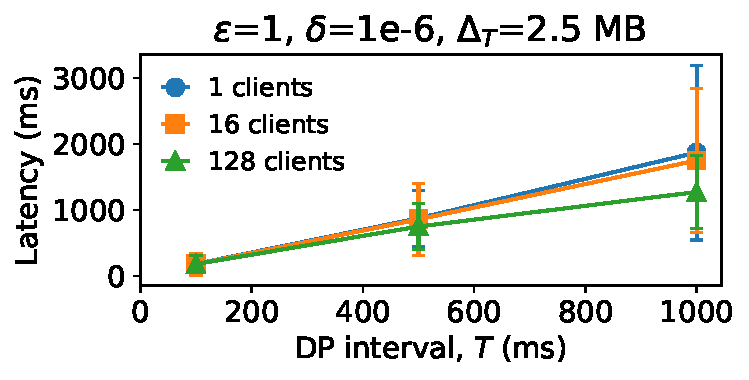
\includegraphics[width=\textwidth]{latency_vs_dp_interval_video_updated.pdf}
      \caption{Latency vs DP interval}
      \label{fig:video-lat-vs-dpInt}
  \end{subfigure}
  \hfill
  \begin{subfigure}[b]{0.49\columnwidth}
      \centering
      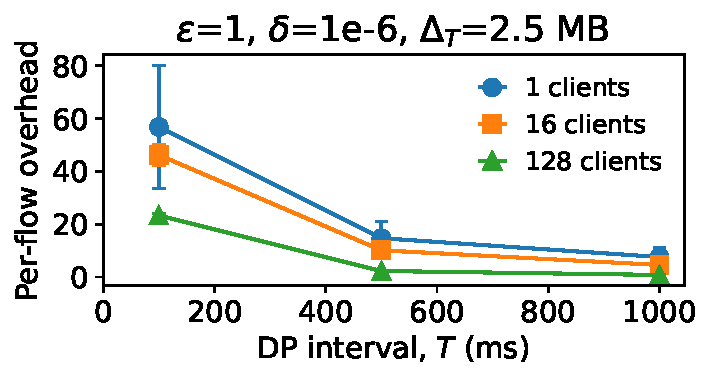
\includegraphics[width=\textwidth]{overhead_vs_dp_interval_video_updated.pdf}
      \caption{BW overhead vs DP interval}
      \label{fig:video-overhead-vs-dpInt}
  \end{subfigure}
  \begin{subfigure}[b]{0.49\columnwidth}
      \centering
      \includegraphics[width=\textwidth]{latency_vs_dp_interval_web_updated.pdf}
      \caption{Latency vs DP interval}
      \label{fig:web-lat-vs-dpInt}
  \end{subfigure}
  \hfill
  \begin{subfigure}[b]{0.49\columnwidth}
      \centering
      \includegraphics[width=\textwidth]{overhead_vs_dp_interval_web_updated.pdf}
      \caption{BW overhead vs DP interval}
      \label{fig:web-overhead-vs-dpInt}
  \end{subfigure}
  \caption{Latency and bandwidth overhead for different values of DP interval for video streaming (a, b) and for web (c, d).}
  \begin{subfigure}[b]{0.485\columnwidth}
      \centering
      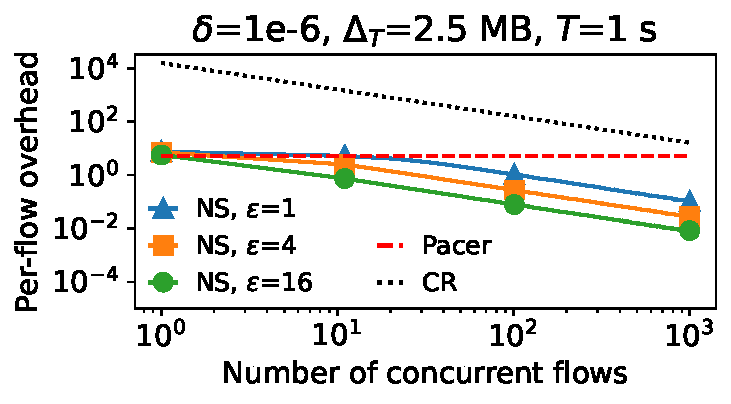
\includegraphics[width=\textwidth]{overhead_vs_number_of_traces_video_bidirectional_loglog_updated.pdf}
      \caption{Video streaming.}
      \label{fig:video-overheads-compare}
  \end{subfigure}
  \hfill
  \begin{subfigure}[b]{0.485\columnwidth}
      \centering
      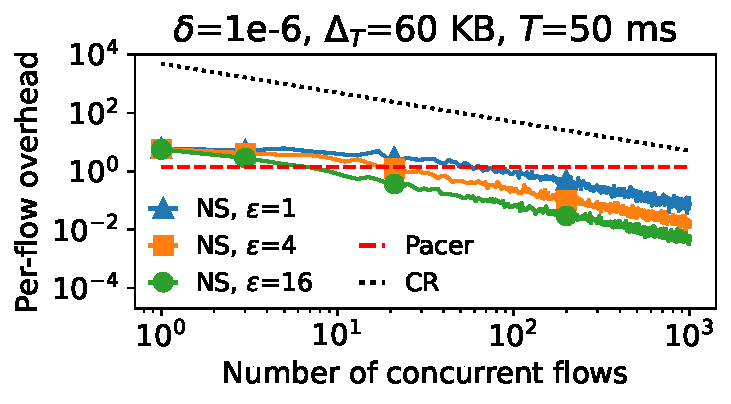
\includegraphics[width=\textwidth]{overhead_vs_number_of_traces_web_bidirectional_loglog_updated.pdf}
      \caption{Web service.}
      \label{fig:web-overheads-compare}
  \end{subfigure}
  \caption{Comparison of {\sys}, constant shaping, Pacer.}
  \vspace{-0.4cm}
\end{figure}
Next, we examine the effect of different privacy settings on bandwidth and
latency overheads for video streaming clients.

%\textbf{Latency vs bandwidth overhead.}
%We configure the DP shaping interval $\dpintvl$ in the middleboxes and
%measure
%the response latencies for individual video segments with the testbed. For the
%same $\dpintvl$ and for a fixed $\ssens$ and $\varepsilon_{\winlen}$, we measure
%the bandwidth overhead for the video streams in the simulator.
We run experiments with three values of $\dpintvl$
for the server: 100ms, 500ms, and 1s, and max per-flow DP length cutoff of
1.21 MB, 1.22MB, and 1.7 MB, respectively. We use
\update{$\qsens = 2.5 MB$} and
\update{$\varepsilon = 1$}.
For all experiments, we set the DP parameters for client request traffic as
follows: \update{$\qsens = 200$}~bytes, $\winlen = 1s$, $\dpintvl = 10ms$,
\update{$\varepsilon = 1$} and max per-flow DP length cutoff of 206 bytes.
We run experiments with 1, 16, and 128 video
clients; each client requests one video randomly selected from the dataset.
For each set of configurations, we measure the average response latency for
individual video segments with the testbed as well as the per-flow relative
bandwidth overhead for the video streams in the simulator.

\textbf{Latency and bandwidth overhead.}
%For each value of $\dpintvl$, we vary video clients between 1 to 16, with each
%client streaming one video randomly selected from the dataset.
%In \update{\Cref{fig:video-lat-vs-xput}},
%the x axis shows the
%%\todo{average and standard deviation} of
%the download latency across all video segments.
%The y axis shows the
%%\todo{average and standard deviation of the per-flow}
%\update{average per-flow}
%relative bandwidth overhead across all videos streamed
%by the concurrent clients.
\Cref{fig:video-lat-vs-dpInt,fig:video-overhead-vs-dpInt} respectively show the
average segment download latency and the average per-flow relative bandwidth
overhead as a function of different intervals and for varying number of clients.
The {\base} segment download latency is \update{2.86 $\pm$ 1.41ms.} The latency
variance is due to variances in the segment sizes.
The relative bandwidth overhead of a video is the
number of dummy bytes transmitted normalized to the size of the unshaped video
stream.
The error bars show the standard deviation in latency and bandwidth overhead.

First, \Cref{fig:video-lat-vs-dpInt} shows that, for all values of $\dpintvl$,
the video segments can be downloaded well within 5s, which is the time to play
each segment and request the next segment from the server.
\update{The high variance is due to negative DP noise, which delays
payload transmission.}
Secondly, the results show the trade-off between latency and bandwidth. A larger
DP interval implies higher download latency but fewer queries, thus
yielding a lower bandwidth overhead.
%Moreover, $\dpintvl = 2.5s$ incurs a total bandwidth overhead of \todo{X MB} for
%a single client.
Thirdly, with multiple concurrent clients, the bandwidth overhead is
amortized, while the average download latency only depends on $\dpintvl$.
Overall, {\sys} can secure video streams with low bandwidth overheads
and no impact on the streaming experience.


\subsection{Case Study: Web Service}\label{subsec:eval-web}
%We analyze the overheads on bandwidth, client response
%latency, and peak server throughput of a web service.
%\begin{figure}[t]
%  \centering
%  \begin{subfigure}{0.49\columnwidth}
%      \centering
%%
%%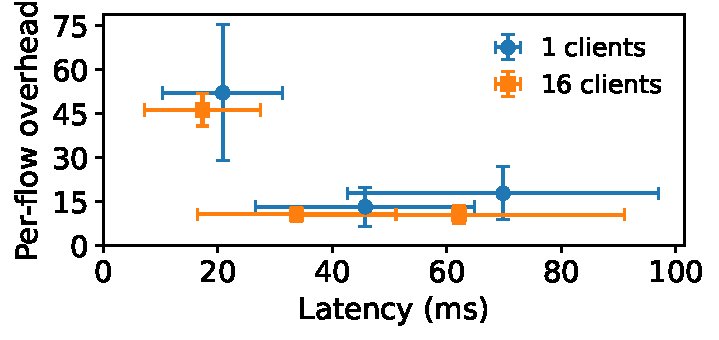
\includegraphics[width=\textwidth]{plots/bw_overhead_vs_latencies_web.pdf}
%
%\includegraphics[width=\textwidth]{plots/latency_vs_dp_interval_web_updated.pdf}
%      \caption{Latency vs DP interval}
%      \label{fig:web-lat-vs-dpInt}
%  \end{subfigure}
%  \hfill
%  \begin{subfigure}{0.49\columnwidth}
%      \centering
%
%\includegraphics[width=\textwidth]{plots/overhead_vs_dp_interval_web_updated.pdf}
%      \caption{BW overhead vs DP interval}
%      \label{fig:web-overhead-vs-dpInt}
%  \end{subfigure}
%  \caption{\update{Web service. Latency and bandwidth overhead for different
%  values of DP interval.}
%  }
%\end{figure}
We perform similar experiments as \S\ref{subsec:eval-video} with our web
service. For the server responses, we use \update{$\qsens = 60 KB$}, $\winlen =
1s$, and \update{$\varepsilon = 1$}. We use $\dpintvl$ of {10ms, 50ms, and
100ms}, and per-flow DP length cutoffs of 60.8KB, 60.8KB, and 110.9KB,
respectively.
For the client requests, we use the same configs as in
\S\ref{subsec:eval-video}. We run \update{3 min} experiments with 1, 16, and 128
wrk2 clients with a total load of \update{1600 req/s};
each client requests random web pages from the dataset. We discard the numbers
of the first minute.

\textbf{Latency and bandwidth overhead.}
%For each value of $\dpintvl$, we vary wrk2 clients between 1 to 16, with each
%client requesting several web pages randomly selected from the dataset.
%\update{\Cref{fig:web-lat-vs-xput}} presents the average response latency versus
%the \update{average per-flow} relative bandwidth overhead across all
%requested pages. The error bars indicate standard deviation.
%
%The figure shows that {\sys} can sustain peak throughput in all configurations.
\Cref{fig:web-lat-vs-dpInt,fig:web-overhead-vs-dpInt} respectively show the
average response latency and the average per-web page relative bandwidth
overhead, across all web page requests.
The {\base} latency is \update{0.225 $\pm$ 0.3 ms}. (The high variance is due to
the time precision in wrk2 being restricted to 1ms.)
%{\ns} latency at peak throughput is $\todo{X} ms$, $\todo{X} ms$, and $\todo{X}
%ms$ with $\dpintvl$ of \todo{0.01ms}, \todo{0.05ms}, and \todo{0.1ms},
%respectively.
The web workload is more sporadic than video streaming, thus web page download
latencies have higher variance than video segment download latency.
The absolute latency overhead for {\ns} depends on the choice of $\dpintvl$. The
relative overhead depends on the underlying network latency, which unlike our
testbed, is in the order of 10s to 100s of milliseconds in the Internet.
%
%The web traffic is much smaller than video streams. Hence, for
%similar privacy loss and number of DP queries, the bandwidth overhead is
%higher for the smaller web traffic.
Interestingly, the bandwidth overhead for web traffic first reduces with
increasing DP shaping interval from 10ms to 50ms, but then increases again
with an interval of 100ms. This is because, for small web pages, the DP interval
of 100ms is larger than the total time required to download web pages. As a
result, additional overhead is incurred due to the padding of traffic in the
100ms intervals.

\subsection{Comparison with other techniques}\label{subsec:eval-comparison}
%\begin{figure}[t]
%  \centering
%  \begin{subfigure}{0.49\columnwidth}
%  \centering
%%
%%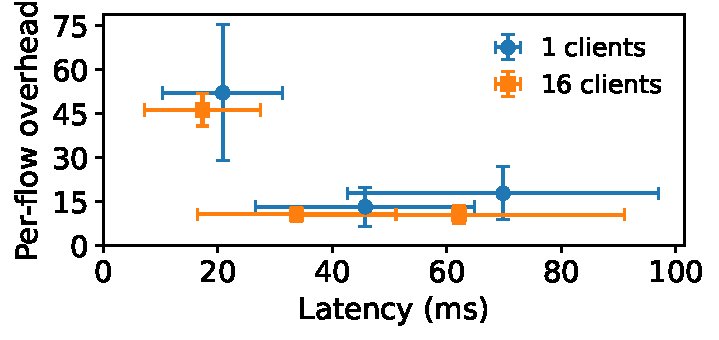
\includegraphics[width=\textwidth]{plots/bw_overhead_vs_latencies_web.pdf}
%
%\includegraphics[width=\textwidth]{plots/overhead_vs_number_of_traces_video_bidirectional_loglog_updated.pdf}
%      \caption{Video streaming.}
%      \label{fig:video-overheads-compare}
%  \end{subfigure}
%  \hfill
%  \begin{subfigure}{0.49\columnwidth}
%      \centering
%
%\includegraphics[width=\textwidth]{plots/overhead_vs_number_of_traces_web_bidirectional_loglog_updated.pdf}
%      \caption{Web service.}
%      \label{fig:web-overheads-compare}
%  \end{subfigure}
%  \caption{\update{Comparison of {\sys}, constant shaping, Pacer.}
%  }
%\end{figure}

%\textbf{Comparison with other techniques.}
\Cref{fig:video-overheads-compare,fig:web-overheads-compare} show the per-flow
relative bandwidth overhead of {\ns},
%(different $\varepsilon$ values),
{\constshape}, and {\pacer} for video and web
applications, respectively, for varying number of concurrent flows.
%We compare overhead of {\ns} with constant rate shaping ({\constshape})
%and~Pacer \cite{mehta2022pacer}.

% For {\constshape}, we configure the peak load for video service corresponding to
% transmitting 1.7MB in every 5s, and the peak load for web service corresponding
% to transmitting 57KB every 50ms. These rates correspond to transmitting at a
% rate that covers the largest object sizes in our video and web datasets.

% In Pacer, for video service, we pad a segment at $i$\textsuperscript{th} index
% in a video stream to the largest segment size at that index across all videos in
% the dataset. For web service, we pad all web pages to the largest page size,
% \ie 147KB in our dataset.

For both video and web traffic, {\ns} incurs three orders of magnitude lower
overhead than {\constshape}, which requires continuously transmitting traffic at
the peak server load (configured for 1000 clients).
%
%For video traffic, {\ns} requires 11 flows to achieve lower overhead than
%{\pacer}.
%For video traffic, while {\ns} incurs similar overhead as Pacer for a single
%flow with \update{$\varepsilon = 1$}, it can further amortize its overheads
%among multiple concurrent streams within the tunnel without compromising
%privacy.
%Specifically, the per-stream overheads become lower than those of
%%{\constshape} and
%Pacer with just \todo{5} streams and are \todo{$ <10\%$} with \todo{10}
%streams.
%\am{It might look like we cherrypicked Pacer for comparison. Maybe
    %Pacer comparison can go.}
%Unlike {\constshape} and Pacer, {\ns} can amortize overheads among
%multiple concurrent streams sharing the same tunnel without compromising
%privacy.
%\Cref{fig:video-overheads-compare} illustrate per-flow bandwidth overhead of
%{\ns} with different values of privacy loss compared to other methods. We use
%an update interval of 1 s, sensitivity of 1 MB, and measure the per-flow
%overhead and privacy loss of segments of 5 s respectively.
%Note that unlike other methods such as Pacer \cite{mehta2022pacer} and constant
%rate shaping, the bandwidth overhead of {\sys} depends on the number of parallel
%flows going through our middlebox.
%Specifically, when a channel of information between two middleboxes became
%differentially private, all flows going through the channel leverage the same
%level of privacy.
%Therefore, the per flow overhead decreases based on the number of flows. For
%example, with about 100 parallel streams going through {\sys} middlebox, the
%per-stream overhead is as small as 10\% of the actual size of streams.
%
%\textbf{Comparison with other techniques.}
%\Cref{fig:web-overheads-compare} shows the relative bandwidth overhead, per web
%request, varying with number of concurrent requests and for different values of
%$\varepsilon_{\winlen}$. Again, the overhead of {\ns} is three orders of
%magnitude lower than that of {\constshape}.
%%Here, {\ns} incurs higher overheads than Pacer,
%For web traffic, {\ns} requires more than \update{40 flows}
%%\update{20 flows at $\varepsilon_{\winlen} =
%%16$} and \update{60 flows at $\varepsilon_{\winlen} = 4$}
%to achieve lower overhead than {\pacer}.
For video and web traffic, {\ns} requires 11 flows and more than 40 flows,
respectively to achieve lower overhead {\pacer}.
Pacer shapes server traffic only upon receiving a client request and does not
shape client traffic. Thus, it leaks the timing and shape of client requests,
which could potentially reveal information about the server responses
\cite{chen2010reality}.
{\sys} shapes traffic in both directions, which incurs higher overhead at the
cost of stronger privacy than Pacer.
%\todo{Explain.}
%Moreover Pacer pads the server response to the largest page length
%in the server's dataset and stops transmitting after a number of packets
%corresponding to the largest page length have been transmitted.
%\todo{In contrast, {\sys} continuously shapes traffic for 1s windows.}
%\am{Need to make this more precise}.





\if 0
\paragraph{Bandwidth overhead vs privacy loss.}
We compare the bandwidth overhead for web traffic due to {\ns}, {\constshape},
and Pacer in \Cref{fig:web-overheads-compare}.
\todo{We use $\winlen = 1 s$, $\dpintvl = 0.1 s$, $\ssens = 150 KB$, and the
same values of $\varepsilon_{\winlen}$ as in \S\ref{subsec:eval-video}, and we
measure the per-flow overhead until each web page is downloaded.}

\todo{Here, {\ns} incurs higher overheads than Pacer because Pacer only pads all
web pages to the largest page length in a service's dataset, whereas {\ns}
performs traffic shaping without any prior knowledge of the page sizes.} \am{Not
convinced about the argument here. $\ssens$ is chosen somewhat based on the
dataset; the overheads would vary based on $\ssens$.}
%We use the same metric of \Cref{subsec:eval-video} to measure the bandwidth
%overhead of {\sys} in shaping traffic of web services with different levels of
%privacy loss. With an update interval of 100 ms and sensitivity of 150 KB, we
%measure the per-flow overhead of {\sys} shaping mechanism and aggregated
%privacy loss for windows of 1 second.

%It is worth noting that the overhead of Pacer \cite{mehta2022pacer} is notably
%low, as it pads all webpages to their maximum size prior to transmission.
%In contrast, {\sys} performs traffic shaping without any prior knowledge of the
%page sizes.
\fi

\smallskip\noindent
\textbf{Evaluation summary.}
{
Our evaluation provides four insights.
(i) There is a huge gap between the theoretical DP guarantees and the
privacy configurations required to defeat SOTA attacks.
%Theoretical analysis suggests that you need quite strong privacy guarantees, but
%from a practical perspective, applications require much weaker guarantees.
%(ii) the costs of privacy required in the face of more sophisticated attacks in
%the future,
(ii) The latency overhead is dominated by the choice of DP shaping interval,
(iii) {\sys}'s middlebox can match about 88\% of the 10Gbps NIC line rate; a
single core of
{\ushaper} can match the peak throughput of a single core server,
(iv) {\sys}'s cost is in the two additional cores for {\prepare} and QUIC worker,
which helps to avoid any secret-dependent interference in shaping and keep low DP
shaping loop lengths. By optimising the implementation, we could use a
single middlebox to support larger workloads.
%The CPU utilization is 3-10\% for the {\prepare} core and depends on the loop
%interval; the utilization is 8-70\% for the QUIC worker core, which depends on
%network I/O. The {\ushaper} core utilizes 100\% of the CPU as it polls for
%packets from {\prepare}. As such, the {\prepare} and QUIC worker cores would be
%able to support additional application cores. By using a polling interval, we
%could reduce the CPU utilization of {\ushaper} to support additional requests at
%the cost of additional latency.
%\am{provide an estimate of scaling the cores.}
%negligible compared to the overheads due to DP shaping.
}

%\section{Limitations and Discussion}
\label{sec:discussion}

We discuss extensions of the {\sys}'s prototype to support additional usages.

\if 0
\paragraph{Multiplexing with non-sensitive flows}
%{\sys} currently assumes that the network paths of non-sensitive and sensitive
%flows are physically isolated. To overcome this limitation, {\sys} can integrate
To route non-sensitive flows alongside sensitive flows, {\sys} can integrate
TDMA (time division multiple access) scheduling \cite{vattikonda2012tdma,
beams2021ifs} in its architecture. Specifically, {\sys} must employ a
synchronous TDMA schedule on its ingress and egress ports and on its CPUs for
each traffic class. When the slot for non-sensitive flows is scheduled, the
traffic is simply routed from the {\sys}’s ingress port to the egress port and
vice versa without any modifications.
%
Note that each tunnel endpoint can use a different TDMA schedule. A synchronous
TDMA schedule between each pair of endpoints may be useful for minimizing
overheads but is not essential for end-to-end security guarantees.
\fi
%\subsection{Alternate deployments of {\sys}}

%\if 0
\textbf{Scheduling multiple tunnels.}
%When handling multiple tunnels, {\sys} must ensure that the
%unshaped traffic of one tunnel is not leaked to another tunnel. Such leaks may
%arise via contention side channels in the mdidlebox.
When handling multiple tunnels, the unshaped traffic of one tunnel could
indirectly affect the shape of traffic in another tunnel, thus potentially
leaking the traffic of the first tunnels.
%For this,
{\sys} must isolate the tunnels from each other in the middlebox.
%Based on \S\ref{sec:implementation}, we require that the {\prepare}
%and QUIC worker threads must be performance isolated from {\ushaper} in each
%tunnel, (ii) the timing of {\prepare} must be masked to secret-independent
%times.
{\sys} could partition the middlebox cores into three groups, each core group
hosting the {\ushaper} process, the {\prepare} threads, and the QUIC worker
threads from different tunnels.
Additionally, {\sys} must use a TDMA schedule among the {\prepare} threads,
while \update{padding} each thread's execution to a secret-independent time.
%In {\sys}, only the {\dshaper} components need to be isolated. {\sys} uses a
%TDMA to schedule the {\dshaper} processes of different tunnels.
Since each {\prepare} thread enqueues shaped buffers at secret-independent
times, QUIC workers of different tunnels can be scheduled to transmit
packets arbitrarily.
%can subsequently %package the buffers into packets and
%transmit the packets in their tunnels following any arbitrary schedule.
%
%{Determining optimal TDMA schedules and their adaptation to the changing
%number of active tunnels is left to future work.}
%\am{Not implemented, remove?}
%\fi

\textbf{Generalization to multi-node communication.}
%\todo{TODO: single application with multiple tiers (e.g., CDNs to serve
%    different parts of a web request) -- general DAG topology}
%\todo{TODO: multi-party communication (e.g., a group VoIP call relayed through a
%    central server) -- star topology}
%{\sys} mitigates network side channel leaks in bidirectional communications
%between a client-server pair. However, {\sys}'s DP shaping can be extended
Some applications may involve multiple nodes forming a communication graph,
where the communication graph could uniquely identify application secrets.
For example, dynamic web pages may be recognized from the traffic generated to
all servers hosting web page components.
%serving dynamic web pages may require downloading embedded objects from
%multiple  servers.
{\sys} can be extended to protect secrets in such applications.
{\sys}'s middlebox is portable and can be easily added in front
of each node to shape traffic on all links.
A client could establish tunnels among all pairs of nodes in an application for
the duration of its interaction with the application.
Each link could use its own DP parameters for shaping; the privacy
guarantees over the communication graph would be a composition of DP guarantees
of all links in the graph.
We leave a detailed analyses of privacy guarantees and overheads in a multi-node
application to future work.
%The key requirement is to model a ``buffering queue'' to define the maximum
%information that could be accessed by an adversary in the communication graph.

\textbf{Integrating {\sys} with end hosts.}
To ensure end-to-end security while accessing sensitive services from outside
organization premises, users could use a VPN client on their devices that is
enhanced with {\sys}'s shaping capabilities. A key challenge would be to ensure
performance isolation of the {\sys}-enhanced VPN client from the application
handling sensitive data \cite{mehta2022pacer}.

\textbf{Integrating {\sys} with other technologies.}
{\sys} can be considered as a network function (NF) and can be integrated with a
chain of other NFs, such as load balancers, firewalls, and intrusion-detection
systems. {\sys} could be the first function in an NF chain, interfacing with the
external network, which forwards inbound flows to other NFs after dropping
padding and shapes only select outbound flows forwarded by the next NF in the
chain. Placing {\sys} at the beginning of the chain would minimize the
communication bandwidth within the NF chain and the private network.
%\am{just mention as a one line somewhere earlier?}
%\paragraph{Interaction between {\sys} and DPI technologies.}
%{\sys} does not conflict with deep packet inspection (DPI) technologies, which
%an organization may use to monitor their inbound traffic for suspicious
%behaviors. However, {\sys} protects against third-party DPI which may


%\subsection{Generalization for orthogonal goals}
%\paragraph{Anonymity.}

\vspace{-0.1cm}
\section{Related Work}
\label{sec:related}

%We discuss prior work on different threat models, goals,
%architectures, and strategies for mitigating network side channels.
%We discuss prior work along three axes: shaping strategy,
%system architecture, and threat model and goals.

\textbf{Traffic shaping for web.}
Prior work used traffic shaping~for defending against website
fingerprinting attacks.
%These strategies can be classified into two types: static and dynamic.
%
Walkie-Talkie \cite{wang2017walkietalkie}, Supersequence
\noindent \cite{wang2014supersequence}, and Glove \cite{nithyanand2014glove} use
clustering techniques to group objects of a corpus and then shape the
traffic of all objects within each cluster to conform to a similar pattern.
Traffic morphing \cite{wright2009morphing} makes the traffic of one page look
like that of another.
These techniques compute traffic shapes that envelope or resemble the network
traces of individual objects. Hence, they require a large number of
traces to account for network variations.
{\sys} dynamically adapts traffic shapes based on the
prevailing network~conditions.
%while conforming with DP guarantees
%and, thus is, computationally less expensive.

%BuFLO~\cite{dyer2012peekaboo},
Cs-BuFLO~\cite{cai2014csbuflo}, Tamaraw~\cite{cai2014tamaraw}, and
DynaFlow~\cite{lu2018dynaflow}, determine traffic shape directly at runtime.
%and FRONT and GLUE~\cite{gong2020zero} are
%dynamic techniques that determine traffic shape at runtime.
They pad object sizes to values that are correlated
with the original object sizes, such as the next
multiple or power of a configurable constant.
%The constants determine
%%the padding overhead and
%the number of objects padded to the same size.
These defenses provide privacy akin to k-anonymity, but have no control on the
the size of the anonymous cluster.
Tamaraw\cite{cai2014tamaraw} formalizes the privacy guarantees.
{\sys}'s DP guarantees are strictly stronger than Tamaraw's (proof
in~\S\ref{appendix:tamaraw}).
%\todo{{\sys} provides a stronger privacy guarantee based on DP (see
%\S\ref{appendix:tamaraw} for a proof).}
%Tamaraw provides a mathematical model to quantify the privacy guarantees of
%fingerprinting defenses.
%
%We prove that their notion of privacy is strictly weaker than differential
%privacy for traffic streams (see \Cref{appendix:tamaraw}).
%FRONT~\cite{gong2020zero} only obfuscates the beginning of the network
%traces of web pages.
%and the gap between consecutive traces, respectively.
%by adding random amount of dummy packets.
%BuFLO and Cs-BuFLO transmit fixed-sized packets at constant rate over a
%predefined duration of time. GLUE is specifically designed to obfuscate the
%beginning and end of a web trace by introducing additional packets between
%traces originating from different webpages.

%Despite extensive profiling, these techniques are unlikely to be able to cover
%all network conditions at runtime.
%{\sys}, on the other hand, is a dynamic traffic shaping solution, which
%provides strong, quantifiable differential privacy guarantees on both packet
%sizes and timing.

\textbf{Differential privacy over streams.}
%\textbf{Differential Privacy.}
%Kellaris et al.~\cite{kellaris2014differentially} also study DP over streams.
%They introduce \textit{$w$-event} privacy based on a neighboring definition that
%only allows stream to differ over {\em one} window $w$.
Dwork et al.~\cite{dwork2010dpcontinual} study DP on streams, in which
neighboring streams differ in at most one element and the query
counts over the stream prefix (without forgetting
old information) under a fixed DP budget for the entire stream.
%is constantly updated over time
%This paper focues on a different setting than ours, in which neighboring streams
%differing in only one element, but the DP query (here a counter) is constantly
%updated over time without forgetting past information (the counter counts the
%whole prefix of the stream), under a fixed DP budget for the entire stream.
{\sys} requires a stronger neighboring definition to model application data
streams (Def. \ref{def:neighboring-streams}), but is able to forget the past by
dropping stale data from our queue (\Cref{assumption:window}) and compose
privacy loss over time.

{\sys}'s neighboring definition is closer to that of user-level DP over streams
in \cite{dwork2010pan}. Instead of counting discrete change,
however, we use the L1 distance which enables coarsening.
Pan-privacy considers an adversary that can compromise the internals of
the algorithms (\eg our buffering queue). This makes the design of algorithms
challenging and costly.
%(the paper provides several impossibility results).
Instead, we consider the buffering queue private and focus on
practical algorithms to study the privacy/overheads trade-off.

%\ml{[I we want to cite pan-privacy] Another work \todo{[cite Pan-privacy]}
%considers user-level DP over streams, which allows for larger changes and is
%closer to our own neighbouring definition (although we use the L1 distance which
%enables coarsening, not counts of discrete change). This paper considers a
%stronger threat model, called PAN-privacy, where an attacker can compromise the
%internals of the algorithms (e.g. our buffering queue). This makes the design of
%algorithms much more challenging and costly (the paper provides several
%impossibility results). Instead, we consider the buffering queue private and
%focus on practical algorithms to study the privacy/utility trade-off.}

Kellaris et al.~\cite{kellaris2014differentially} introduce a notion of DP,
called $w$-event privacy, for streams of length $w$.
%Each event in a stream is~a query result on a static database state at a
%specific timestamp.
Neighboring stream pairs are those whose individual events are pairwise
neighbors within a window of upto $w$.
%Neighboring streams are otherwise identical.
%This is not a practical neighboring definition for the
%streams we consider, and would provide weak privacy.
%{\sys}'s ``database'' consists of video streams and its
{\sys}'s neighboring definition accounts for the maximum stream distance over
{\em any} window of length $\winlen$, which is a better match for the streams
we consider.
%{\sys} also uses the L1-norm distance between streams, whereas $w$-event privacy
%considers the number of differences for discrete elements.

%\ml{Not doing it as I'm not sure if there are other reasons, but I suggest
%    moving this one last of this section.}
%In a similar work,
Zhang et al.~\cite{zhang2019statistical} generate differentially private shapes
for video streams using Fourier Perturbation Algorithm (FPA)
\cite{rastogi2010differentially}.
FPA transforms a finite time series of bursts, into a series of DP shaped bursts
of the same length.
FPA requires the entire stream's profile upfront, and cannot guarantee complete
transmission of an input stream within the shaped trace.
%Unlike {\sys}'s dynamic shaping mechanism, however, FPA requires predefined
%time series associated with traffic traces in advance.
{\sys}'s DP guarantees simply compose over burst interval sequences, thus
allowing shaping of streams of arbitrary lengths with
quantifiable privacy and overheads.
%{\sys} does not constrain transmission duration; rather it can provide DP
%guarantees composed over burst interval sequences of arbitrary lengths.
%{\sys} dynamically shapes bursts in periodic intervals; the DP guarantees
%compose over burst-interval sequences of arbitrary lengths.
%Moreover, it is not guaranteed that the FPA algorithm's output will have
%sufficient capacity (in terms of number of bytes) to accommodate the input
%traffic trace. Authors refer to this issue as deficit phenomena.




%\paragraph{Mitigations for VoIP.}

%\paragraph{Network side-channel mitigation in IoT traffic.}

%\if 0
%%%%%%%%%%%%%%%%%%%%%%%%%%%%%%%%%%
%% remove due to space constraints
%% point covered in intro
%%%%%%%%%%%%%%%%%%%%%%%%%%%%%%%%%%
\textbf{Adversarial defenses.}
%Given the recent advancements in machine learning-based traffic analysis
%attacks, new defensive mechanisms based on adversarial examples have emerged.
%Mockingbird~\cite{rahman2020mockingbird} and Dolos~\cite{shan2021dolos} attempt
%to defeat existing classifiers using adversarial inputs.
%Dolos~\cite{shan2021dolos} computes input-agnostic adversarial patches of dummy
%packets.
%Mockingbird~\cite{rahman2020mockingbird} uses an optimization problem to make
%one stream look like another by adding adversarial inputs to the input stream.
Adversarial defenses~\cite{rahman2020mockingbird, hou2020wf, abusnaina2020dfd,
shan2021dolos, nasr2021defeating, gong2022surakav}
generate targeted and low-overhead noise to defeat specific classifiers.
%attempt to defeat existing classifiers with small amounts of carefully-crafted
%perturbations in the input streams.
%The targeted noise incurs less overhead but cannot defeat another classifier.
%However, the adversarial examples generated for one classifier may not
%generalize to another classifier.
%However, an adversary can train its classifier with adversarial
%samples to become resilient to defenses.
%Thus, this approach leads to an arms race between attackers and defenders.
{\sys} provides provable and configurable privacy against both SOTA as
well as future classifiers.
%\fi


\if 0
%%%%%%%%%%%%%%%%%%%%%%%%%%%%%%%%
%% skip due to space constraints
%%%%%%%%%%%%%%%%%%%%%%%%%%%%%%%%
\paragraph{Mitigations for contention-based network side channels.}
An adversary may be colocated with a victim in the same network and may share
links with a victim’s traffic (e.g., a tenant VM colocated on a Cloud server or
rack). In such a scenario, the adversary can induce contention with the victim’s
traffic on a shared link and use the resulting variations in its own traffic
shape to infer the victim’s traffic shape and ultimately the victim’s secrets.
Such leaks can be mitigated using TDMA
scheduling on the shared links \cite{vattikonda2012tdma, beams2021ifs},
%or by physically isolating the network of the tenants,
which eliminates the
adversary’s ability to observe the victim’s traffic. {\sys} focuses
on an orthogonal threat model where the adversary is privileged and owns (a
part) of the victim’s network path (\eg ISP). It may be infeasible for a tenant
to achieve isolation from the adversary (ISP); thus, {\sys} leverages traffic
shaping to protect the victim’s traffic in the face of adversarial observations.
\fi

\textbf{Network side-channel mitigation systems.}
%\textbf{Pacer.}
%Pacer \cite{mehta2022pacer} proposes the idea of a cloaked tunnel, which is
%conceptually similar to {\sys}’s shaping tunnel.
{\sys}'s shaping tunnel is conceptually similar to Pacer's~\cite{mehta2022pacer}
cloaked tunnel.
%However, they are similarity ends there.
%have different threat models.
%First,
However, Pacer mitigates leaks of a Cloud tenant's secrets to a
colocated adversary through contention at shared network links.
%Thus, Pacer's tunnel endpoint must be integrated with end hosts.
Pacer's cloaked tunnel controls the transmit time of
TCP packets in accordance with the shaping schedule and congestion control
signals. Thus, Pacer requires
non-trivial changes to the network stack on the end hosts.
%First, Pacer’s focus is on an adversary colocated with an application on the end
%host, which infers the application’s traffic shape through indirect
%contention-based side channels.
%Secondly, Pacer implements pacing below the transport layer, which forces it to
%implement congestion awareness in the pacing component. Therefore, Pacer’s
%tunnel endpoint is tightly integrated with end hosts and requires non-trivial
%changes to the network stack on the end hosts.
%
%In {\sys} protects the traffic of applications from an adversary on the public
%Internet.
{\sys} protects applications that are behind private networks but communicate
using the public Internet.
{\sys}'s tunnel endpoints can be placed at the interface of
the private-public networks, \eg in a middlebox, thus supporting
multiple applications without modifying end hosts.
Moreover, by shaping above the transport layer, {\sys} needs to control only the
precise timing for generation of bursts of DP length and not the subsequent
%packetization and
transmission to the network.
%Thus, {\sys}'s design is more modular and portable than Pacer's.

%Besides the tunnel architecture, the
%The shaping strategies of Pacer and {\sys} differ as well.
%Pacer splits a server's dataset into clusters of a minimum size $k$, while
%minimizing padding overhead for the dataset. For each cluster, Pacer then
%computes a traffic shape based on network traces of all cluster objects.
%Pacer's clustering may not suffice to protect objects within the clusters
%against an adversary with information about the popularity of objects within the
%cluster.
%{\sys}'s DP shaping guarantees privacy even against a strong adversary with
%auxiliary information.
%\todo{{\sys}'s overheads are comparable to Pacer's.}
%Pacer assumes that the shape of clients' requests to services is non-sensitive
%and thus shapes only the server responses. Furthermore, Pacer clusters a
%server's dataset into clusters of a minimum size k, while minimizing padding
%overhead for the dataset. These assumptions and optimizations may not suffice
%when an adversary has auxiliary information, such as the popularity of
%individual objects during different times of the day. {\sys}’s DP shaping hides
%the timing as well as the content of the traffic even from a strong adversary
%with access to auxiliary information.
%\todo{Despite the stronger privacy guarantees, {\sys}’s overheads are comparable
%to Pacer's.} {\as{does that mean our guarantees are stronger than pacer? in
%that case I don't think it is correct.}}

Ditto~\cite{meier2022ditto} and {\sys} propose shaping traffic at network nodes
separate from end hosts.
%Ditto~\cite{meier2022ditto} implements shaping in programmable switches, while
{\sys} proposes a hardware-independent, modular and portable
middlebox architecture that can be integrated with end hosts, routers,
gateways, or even programmable switches as in Ditto.
%{\sys}'s middlebox architecture is hardware-independent, modular and portable,
%and can be integrated with either end hosts or intermediate nodes, such as
%routers, or gateways.

%\todo{
%%Ditto defines a sequence of packet sizes and send packets at fixed
%%interval regardless of the size and timing of application packets.
%%It pads application packets to ensure that their sizes follow the predefined
%%sequence and buffers them to maintain the fixed packet interval.
%Unlike Ditto, {\sys} dynamically shapes traffic based on application traffic
%while maintaining DP guarantees.
%}

%\textbf{Censorship circumvention proxies.}
\textbf{Systems with other goals.}
%Tor \cite{Tor}, FTE \cite{dyer2013protocol}, Scramblesuit
%\cite{winter2013scramblesuit}, Skypemorph \cite{mohajeri2012skypemorph}, Balboa
%\cite{rosen2021balboa}, DeltaShaper \cite{barradas2017deltashaper}, and Protozoa
%\cite{barradas2020poking} are
Censorship circumvention systems~\cite{mohajeri2012skypemorph,
winter2013scramblesuit, barradas2017deltashaper,
barradas2020poking, rosen2021balboa}
rely on traffic obfuscation, scrambling, and transformations of a sensitive
application’s shape to that of a non-sensitive application. These techniques
prevent identification of original protocols by deep packet inspection,
but do not prevent inference of secrets from traffic shapes.
%Unlike {\sys}, they do not prevent inference of secrets from traffic shapes.
%They rely on Pluggable Transports (PTs), which is a SOCKS proxy-based
%architecture. PTs run on application end hosts or on trusted nodes in the Tor
%network and communicate over HTTP(S).
%In contrast, {\sys} ensures privacy of the traffic content from an adversary.
%{\sys}'s design is modular and portable.
%For instance, it can integrate a SOCKS proxy in the {\ushaper} process, although,
%its own transport-layer proxy can accept arbitrary application protocols.

\if 0
%%%%%%%%%%%%%%%%%%%%%%%%%%%%%%%%%%%%%
%% remove due to space constraints
%% points covered in intro and design
%%%%%%%%%%%%%%%%%%%%%%%%%%%%%%%%%%%%%
QCSD~\cite{smith2022qcsd} is a client-side only defense framework for website
fingerprinting attacks. QCSD instructs the server about sending payload or dummy
data using flow control signals in the headers of the QUIC packets sent from the
client. Moreover, it uses QUIC's PADDING frames to transmit dummy data.
Unlike the STREAM frames, PADDING frames do not generate
acknowledgements \cite{rfc9000} and, thus, are distinguishable on the network.
Overall, QCSD is a best-effort approach and cannot provide {\sys}'s guarantees.
%To shape the traffic from the server to the client, it leverages the per-stream
%flow control of QUIC to determine when to send actual data, dummy data, or a
%combination of both.
%It is important to note that QCSD is a best-effort approach and does not
%provide a guarantee that the traffic shaping will perfectly match the defense
%mechanism in either directions. Therefore, the QCSD framework is not
%appropriate for emulating the traffic shaping mechanism of {\sys}.
\fi

\if 0
\paragraph{Limitations of QUIC features.}
An alternative design approach is to utilize QUIC padding frames instead of
introducing a separate dummy stream to the connection. However, as stated in the
QUIC specification~\cite{rfc9000}, padding frames are not acknowledged by the
receiver. This poses a significant challenge for us since we require all events
observable by potential adversaries, including ACK messages, to be independent
of the content of streams.
MASQUE (Multiplexed Application Substrate over QUIC Encryption) is a framework
that facilitates the simultaneous execution of multiple networking applications
within an HTTP/3 connection and enables a QUIC client to negotiate proxying
capabilities with an HTTP/3 server.
While MASQUE currently lacks a stable specification and implementation, it holds
potential for providing negotiation capabilities for {\sys} in the future.
\fi

%\textbf{Metadata private communication.}
%\textbf{Anonymous communication.}
Karaoke~\cite{lazar2018karaoke} and Vuvuzela~\cite{van2015vuvuzela} are
anonymous messaging systems that use~DP to hide participants in a conversation,
but use constant-rate traffic among the participants.
\update{
AnoA~\cite{backes2013anoa} is a framework to analyze anonymity
properties of anonymous communication
protocols. AnoA supports DP based quantification for various
properties, such as sender anonymity and sender unlinkability.
%AnoA~\cite{backes2013anoa} is an anonymity analysis framework that establishes
%quantifiable and comparable anonymity properties, taking inspiration from
%privacy frameworks such as differential privacy.
%AnoA provides metrics to quantitatively assess the anonymity provided by an
%Anonymous Communication Protocol.
}
%differential privacy to hide  participants  in a message
%conversation, but rely on constant traffic shaping  among the participants.
{\sys}'s differentially-private traffic shaping hides the traffic content. In
principle, {\sys} could be combined with an anonymous communication system to
provide both content privacy and anonymity with~DP.

%\todo
%{
%\paragraph{Other Methods (To Add).}
%\begin{enumerate}
%\item DFD~\cite{abusnaina2020dfd}: Stochastically extends the size of traffic
%bursts to confuse the classifier.
%\item WF-GAN~\cite{hou2020wf}: Using a Generator/Discriminator to add
%adversarial noise to traffic such that the classifier missclassifies the input.
%\item Mockingbird~\cite{rahman2020mockingbird}: Molds traffic sequence to match
%Adversarial Example sequences generated against an effective Deep Learning
%classifier.
%\item Dolos~\cite{shan2021real}:injects dummy packets into traffic traces by
%computing input-agnostic adversarial patches that disrupt deep learning
%classifiers used in WF attacks. Patches are applied in real time and
%parameterized by a user-side secret, ensuring that attackers cannot use
%adversarial training to defeat Dolos.
%\end{enumerate}
%}

\section{Conclusion}
\label{sec:conclusion}

{\sys} is a provably secure network side-channel mitigation system that provides
quantifiable and tunable privacy guarantees in traffic shaping.
\todo{We believe that {\sys} can eliminate the arms race in {\nsca} attacks and
defenses and can provide a portable and configurable framework for deploying
mitigations for applications with diverse traffic characteristics and in
different settings.}
{\sys}'s DP based traffic shaping strategy as well as its
modular and portable tunnel design can be extended to mitigate leaks
in multi-node systems, but we leave the details to future work.

\section{Acknowledgments}
We thank the USENIX Security reviewers and our shepherd for their constructive
feedback.
This work was supported in part by the Natural Sciences and Engineering Research
Council of Canada (NSERC) [RGPIN-2021-02961, DGECR-2021-00098,
DGDND-2021-02961], the Department of National Defense (DND) [MN3-011], a
Google Research Scholar award, the Digital Research Alliance of Canada, and AWS
(through the UBC Cloud Innovation Center).
%We are also grateful for the support provided by AWS through the UBC Cloud
%Innovation Center.
%(alliancecan.ca).
%We acknowledge the support of the Natural Sciences and Engineering Research
%Council of Canada (NSERC) funding reference numbers DGECR-2022-00400, XXX], and
%funding form a Google Research Scholar award.
%This research was enabled in part by support provided by the Digital Research
%Alliance of Canada (alliancecan.ca).


%\newpage
{
\footnotesize
\bibliographystyle{abbrv}
\bibliography{paper}
}
%\bibliographystyle{abbrv}


\appendix

\section{Attack classifiers}
\label{appendix:tcn}

{\small
\textbf{Beauty and Burst.}
The Beauty and the Burst classifier (BB) \cite{schuster2017beautyburst} is a CNN
(convolutional neural network) consisting of three convolution layers, a max
pooling layer, and two dense layers. We use a dropout of 0.5, 0.7, and 0.5
between the hidden layers of the network. We train the classifier with an Adam
optimizer, a categorical cross-entropy function, a learning rate of 0.01, with a
batch size of 64, and for 1000~epochs.
%\am{Show a figure?}
}

\begin{figure}[t]
    \centering
    \includegraphics[width=\columnwidth]{TCN_arch.pdf}
    \caption{TCN classifier}
    \vspace{-0.4cm}
    \label{fig:tcn}
\end{figure}

{\small
\textbf{Temporal Convolution Network.}
%Recent work has proposed CNN-based classifiers for performing network
%side-channel attacks on video streams.
%While CNNs are generally effective in sequence modeling, there are two problems
%that limit their efficiency in the context of network side-channel attacks.
%First, the convolutional layers applied to a sequence are not inherently causal;
%therefore, they look into future samples of a sequence to decide the output for
%the current sample. Secondly, the effective history of past samples used by CNNs
%is bounded by the number of samples the kernel can cover, meaning the CNNs also
%lack a deep effective history size of past samples in the sequence.
%
While CNNs are generally effective in sequence modelling, they look at future
samples in a sequence and a very limited history of past samples to decide the
output of the current sample. Consequently, they require a large number of traces
and long traces for effective training and prediction.

%While CNNs are generally effective in sequence modeling, there are two problems
%that limit their efficiency in the context of network side-channel attacks.
%First, the convolutional layers need to look into future samples of a sequence
%to decide the output for the current sample, implying that they require long
%traces for effective training. Secondly, they use a limited history of past
%samples as part of training.
Temporal Convolutional Networks (TCNs) \cite{bai2018tcn} overcome these problems
of CNNs by utilizing a one-dimensional fully-convolutional network equipped with
causal dilated convolutions, which allows them to examine deep into the past to
produce an output for the sequence at any given moment.

\Cref{fig:tcn} shows the architecture of our TCN classifier, which follows the
architecture proposed by Bai et al. \cite{bai2018tcn}. It
consists of two dilated causal convolutional layers, followed by weight
normalization and dropout layers with a dropout probability of 0.05. We train
the classifier for 1000 epochs.
%\am{Show a figure?}
}

%\paragraph{Attack setup.}

\if 0
Convolutional neural networks have been shown to be effective in sequence
modelling for decades [1]. However, there are two problems with using a
convolutional neural network as a sequence modeller. First, convolutional layers
applied to a sequence are not inherently causal, meaning that they look into
future samples of a sequence to decide the output for the current sample.
Secondly, in contrast to recurrent neural networks(RNNs) [2], convolutional
neural networks lack a deep effective history size of past samples in the
sequence (i.e. their effective history is bounded to the number of samples that
kernel can cover from the past). To address these problems, Bai et al. [3]
proposed a new architecture called Temporal Convolutional Network (TCN). The TCN
utilizes a one-dimensional fully-convolutional network [4] equipped with causal
dilated convolutions [5], allowing it to examine deep into the past to produce
an output for the sequence at any given moment.  To further stabilize deep and
large TCNs, they added a generic residual block from input to output. The
architecture is shown in the following figure (it will be re-plotted for the
paper).
\fi
\section{Extended evaluation of privacy vs overheads}
\label{sec:eval-extended}

\begin{figure}[t]
    \centering
    \begin{subfigure}{0.49\columnwidth}
      \includegraphics[width=\textwidth]{neighboring_distances_barplot_video.pdf}
%      \caption{Video streaming}
%      \label{subfig:sensitivity-comparison-video}
    \end{subfigure}
    \hfill
    \begin{subfigure}{0.49\columnwidth}
      \includegraphics[width=\textwidth]{neighboring_distances_barplot_web.pdf}
%      \caption{Web service}
%      \label{subfig:sensitivity-comparison-web}
    \end{subfigure}
    \caption{\update{Distribution of the difference in buffering queue lengths
    for application stream pairs.}
    }
    \vspace{-0.2cm}
    \label{fig:sensitivity-comparison}
\end{figure}

\begin{figure}[t]
    \centering
    \begin{subfigure}{0.49\columnwidth}
        \includegraphics[width=\textwidth]{privacy_loss_VS_noise_std_low_sensitivity_updated.pdf}
        \caption{Noise vs privacy loss}
        \label{subfig:low-sens-epsilon-sigma}
    \end{subfigure}
    \hfill
    \begin{subfigure}{0.49\columnwidth}
        \includegraphics[width=\textwidth]{privacy_loss_VS_noise_std_high_sensitivity_updated.pdf}
        \caption{Noise vs privacy loss}
        \label{subfig:high-sens-epsilon-sigma}
    \end{subfigure}
    \hfill
    %\begin{subfigure}{0.32\textwidth}
    %      \centering
    %
    %\includegraphics[width=\textwidth]{privacy_loss_VS_sensitivity_high_sensitivity.pdf}
    %      \caption{Sensitivity vs privacy loss}
    %      \label{subfig:high-sens-epsilon-sensitivity}
    %      \end{subfigure}
\begin{subfigure}{0.49\columnwidth}
    \includegraphics[width=\textwidth]{privacy_loss_VS_query_num_low_sensitivity_updated.pdf}
    \caption{\# DP queries vs privacy loss}
    \label{subfig:low-sens-epsilon-queries}
\end{subfigure}
\hfill
\begin{subfigure}{0.49\columnwidth}
    \includegraphics[width=\textwidth]{privacy_loss_VS_query_num_high_sensitivity_updated.pdf}
    \caption{\# DP queries vs privacy loss}
    \label{subfig:high-sens-epsilon-queries}
\end{subfigure}
%    \begin{subfigure}{0.32\textwidth}
    %    \centering
    %
    %
    %\includegraphics[width=\textwidth]{plots/privacy_loss_VS_sensitivity_low_sensitivity.pdf}
    %    \caption{Sensitivity vs privacy loss}
    %    \label{subfig:low-sens-epsilon-sensitivity}
    %    \end{subfigure}
\caption{
    \update{Privacy loss vs noise and \# queries for different~$\qsens$.}
    %        Relation between per-window loss ($\varepsilon_\winlen$), noise
    %        ($\sigma_\winlen$), sensitivity ($\ssens$), and number of DP
    %        queries ($\varnumupdates$).
}
\vspace{-0.4cm}
\label{fig:privacy-microbenchmarks-extended}
\end{figure}

{\small
%\Cref{subfig:sensitivity-comparison-video,subfig:sensitivity-comparison-web}
\textbf{Distribution of queue length differences.}
\Cref{fig:sensitivity-comparison} shows the distribution of the
buffering queue length differences generated for each pair of an
application's streams. We use $\winlen$ of 5s
for video streams and 1s for web pages.
%The error bars show the min and max differences, the boxes show the first and
%third quartiles.
The dashed lines show the median, which is \update{1.63 MB} and
\update{6 KB} for videos and web pages, respectively.

\textbf{Privacy loss vs overheads for other \update{$\qsens$}.}
\Cref{fig:privacy-microbenchmarks-extended} shows similar results as
\Cref{fig:privacy-microbenchmarks} for \update{$\qsens$} of 0.1 MB and 10 MB.
%of 0.1 MB and 10 MB.
%the relation between $\varepsilon$, $\sigma_\dpintvl$, $\varnumupdates$ for
%$\ssens$ of 0.1 MB and 10 MB.
%at a lower scale of sensitivity ($\ssens$) for two different
%setups: applications with high sensitivity values (e.g. 10 MB) where the queue
%size undergoes significant changes across different streams and applications
%with low sensitivity (e.g. 0.1 MB).
}


{\small
\textbf{Bandwidth overheads with a fixed cutoff.}
In \S\ref{sec:eval}, we explained that {\sys} applies a cutoff to the DP
shaped buffer length (if the sampled noise is very large) that depends on the
number of active flows. This reveals the number of active flows at any given
time.
To hide the number of flows, we can set
the cutoff to a fixed~value (\eg based on the
maximum flows that the system must support).

\Cref{subfig:bw-vs-dpInt-video-no-max} presents results similar to those of
\Cref{fig:video-overhead-vs-dpInt}, but with the cutoff for the shaped buffer
length set to a fixed value of 1.21 GB, 1.22 GB, and 1.7 GB.
%(corresponding to 1000 flows).
%for the three DP intervals.
\Cref{subfig:bw-vs-dpInt-web-no-max} presents results similar to those of
\Cref{fig:web-overhead-vs-dpInt} but with cutoffs of 60.8~MB, 60.8~MB, and 110.9
MB.
%
\Cref{subfig:bw-comparison-video-no-max,subfig:bw-comparison-web-no-max} show
the results similar to those of
\Cref{fig:video-overheads-compare,fig:web-overheads-compare}.
%the relative bandwidth overhead of {\ns} compared with {\pacer} and
%{\constshape}.
%In comparison with Pacer, for a small number of parallel flows, {\sys}'s
%bandwidth overhead increases significantly. However, with multiple concurrent
%flows, the amortization effect exponentially reduces overhead.
%
The fixed cutoffs correspond to 1000 flows, which lead to a significant increase
in {\sys}'s overheads.
However, the overheads quickly amortize with several concurrent flows.
}
%\Cref{subfig:bw-vs-dpInt-video-no-max} shows the relative bandwidth overhead of
%our video streaming application for different DP intervals with the shaped
%buffer length cutoff set to 1000 flows.
%Compared to \Cref{fig:video-overhead-vs-dpInt}, {\sys}'s bandwidth overhead
%increases significantly with a fixed cutoff.
%However, the overheads quickly amortize with larger number of concurrent flows.
%%when operating with just a single client, often reaching two orders of
%%magnitude higher values.
%%However, the overheads remain relatively the same when a large number of
%%clients are present (e.g., 128 or more).
%\Cref{subfig:bw-vs-dpInt-web-no-max} represents the similar results for the web
%service.

\begin{figure}[t]
    \centering
    \begin{subfigure}{0.49\columnwidth}
        \centering
        \includegraphics[width=\textwidth]{overhead_vs_dp_interval_video_updated_no_max.pdf}
        \caption{Video streaming}
        %        \caption{Noise vs privacy loss}
        \label{subfig:bw-vs-dpInt-video-no-max}
    \end{subfigure}
    \hfill
    %    \begin{subfigure}{0.33\textwidth}
        %        \centering
        %
        %\includegraphics[width=\textwidth]{plots/privacy_loss_VS_sensitivity_video.pdf}
        %        \caption{Sensitivity vs privacy loss}
        %        \label{subfig:high-sensitivity-epsilon-sensitivity}
        %    \end{subfigure}
    %    \hfill
    \begin{subfigure}{0.49\columnwidth}
        \centering
        \includegraphics[width=\textwidth]{overhead_vs_dp_interval_web_updated_no_max.pdf}
        \caption{Web service}
        %        \caption{\# of DP queries vs privacy loss}
        \label{subfig:bw-vs-dpInt-web-no-max}
    \end{subfigure}
    %  \caption{
        %    \update{Bandwidth overheads with a fixed cutoff.}
        %%    \am{Make notations consistent.}
        %  }
    %\end{figure}


    %\begin{figure}[t]
    \centering
    \begin{subfigure}{0.49\columnwidth}
        \centering
        \includegraphics[width=\textwidth]{overhead_vs_number_of_traces_video_bidirectional_loglog_updated_no_max.pdf}
        \caption{Video streaming}
        %        \caption{Noise vs privacy loss}
        \label{subfig:bw-comparison-video-no-max}
    \end{subfigure}
    \hfill
    %    \begin{subfigure}{0.33\textwidth}
        %        \centering
        %
        %\includegraphics[width=\textwidth]{plots/privacy_loss_VS_sensitivity_video.pdf}
        %        \caption{Sensitivity vs privacy loss}
        %        \label{subfig:high-sensitivity-epsilon-sensitivity}
        %    \end{subfigure}
    %    \hfill
    \begin{subfigure}{0.49\columnwidth}
        \centering
        \includegraphics[width=\textwidth]{overhead_vs_number_of_traces_web_bidirectional_loglog_updated_no_max.pdf}
        \caption{Web service}
        %        \caption{\# of DP queries vs privacy loss}
        \label{subfig:bw-comparison-web-no-max}
    \end{subfigure}
    \caption{
        \update{Bandwidth overheads with a fixed cutoff.}
        %    \am{Make notations consistent.}
    }
\vspace{-0.4cm}
    %  \caption{
        %    \update{Comparison of {\sys}, constant shaping, Pacer with a fixed
        %cutoff.}
        %%    \am{Make notations consistent.}
        %  }
\end{figure}


\section{Proof of {\sys}'s DP based Shaping}
\label{appendix:dp}

% \am{Revise annotations.}

% \begin{algorithm}[t]
%     \caption{{\sys} DP traffic shaping}
%     \label{alg:dp_shaping_mechanism}
%     \begin{algorithmic}[1]
%         \While {\textbf{not} end of data transmission}
%         \State $\tau$ = \texttt{current\_time()}
%         %
%         \State $\unshapedQ_{\tau}$ = \texttt{get\_size()}
%         %
%         \State $\tilde{\unshapedQ}_{\tau}$ = $\unshapedQ_{\tau} +
%         \mathcal{N}\big(0,
%         \frac{2\Delta}{\varepsilon}\ln(\frac{1.25}{\delta})\big)$ \;
%         %
%         \State \texttt{dequeue($\tilde{\unshapedQ}_{\tau}$)}
%         \State \texttt{sleep($T$)}
%         \EndWhile
%     \end{algorithmic}
% \end{algorithm}

% \begin{assumption*}\label{assumption:window_appendix}
%   All bytes enqueued at time $t$ are transmitted by time $t+W$.
% \end{assumption*}


% \begin{proposition}\label{prop:sensitivity-bound}
  % {$\sys$} enforces $\qsens \leq \ssens$.
% \end{proposition}

{\small
\begin{numprop}[\ref{prop:sensitivity}]
  {$\sys$} enforces $\qsens \leq \ssens$.
\end{numprop}
\noindent To prove \Cref{prop:sensitivity}, we show that at any DP query time
$k$, any neighboring streams $\istream, \istream'$ can only create a queue size
difference such that $|\qlent{k} - \qlent{k}'| \leq \ssens$. This is formalized
in the following Lemma:
\begin{lemma}\label{lemma:sensitivity-time}
Assume two neighboring traffic streams $\istream$ and $\istream'$
($\|\istream-\istream'\|_1 \leq \ssens$), are transmitted through {\sys} and
get the same randomness draws $z_k$ (they are parallel worlds with an identical
  \sys, but the streams differ).
Then, at any DP query time $k$, the length of the buffering queue for
  $\istream$ and $\istream'$ are $\ssens$-close.
Formally:

\begin{equation}\label{equ:composition}
        \forall k \geq 0 : |\qlent{k} - \qlent{k}'| \leq \ssens
\end{equation}
\end{lemma}
\begin{proof}
{\sys} performs a DP query for the size of the buffering queue at intervals of
length $T$.
While transmitting $\istream$, the queue length at the end of the
$k$\textsuperscript{th} interval $\dpintvl_{k}$ is a function of three
variables:
%
%\begin{enumerate}
(i) The buffering queue length $\qlent{k-1}$ at the end of
$\dpintvl_{k-1}$.
%
(ii) The total number of payload bytes that have been dequeued from the
buffering queue in the $k$\textsuperscript{th} interval,
${\payload}_{k}$.
%
(iii) The number of new payload bytes from the application stream added
to the buffering queue since the previous interval, which is the sum of
sizes of all packets arriving between $(k-1)$\textsuperscript{th} and
$k$\textsuperscript{th} interval, \ie
%        $\sum_{T_{k-1} \leq t < T_k} P^S_t$
$\sum_{\dpintvl_{k-1} \leq t < \dpintvl_{k}} P^S_t$.
%
%\end{enumerate}
% As $\istream$ and $\istream'$ are reshaped to the same $\ostream$,
% the shaped buffer length for the two streams is the same in all intervals (i.e.
% $\forall k
% \geq 0 : \qlendpt{k} = \qlendpt{k}'$).
%
Therefore, the buffering queue length after dequeue in $\dpintvl_{k}$ is:
\begin{equation}\label{equ:queue-state}
\qlent{k} = {\qlent{k-1}} +
{\sum_{\dpintvl_{k-1} \leq t < \dpintvl_{k}} P^S_t}
%{\sum_{T_{k-1} \leq t < T_k} P^S_t}
-
{{\payload}_{k}}
\end{equation}
%\\
The difference between the queue lengths of
$\istream, \istream'$ at $\dpintvl_{k}$ is:
{\footnotesize
\begin{equation}\label{equ:queue_state_expansion}
\qlent{k} - \qlent{k}'~=~(\qlent{k-1} - \qlent{k-1}')~+ (\sum_{\dpintvl_{k-1} \leq t < \dpintvl_{k}}P^S_t - \sum_{\dpintvl_{k-1} \leq t < \dpintvl_{k}}P^{S'}_t) - ({\payload}_{k} - {\payload}_{k}')
\end{equation}}
We divide the proof into two steps.
First, we show that the dequeue stage of the shaping mechanism does not increase the difference in queue lengths.
Secondly, we show that under \Cref{assumption:window}, the enqueue stage of incoming streams does not increase the difference in queue lengths beyond $\ssens$.

% Given that $\istream$ and $\istream'$ are reshaped to the same output
% stream $\ostream$, the sizes of output packets generated in each interval
% $\dpintvl$ when transmitting either streams is the same. However, the
% content of the output packets in each stream may differ based on the sizes and
% timing of the packets in each input stream.
% This implies that the number of payload bytes dequeued from the buffering queue
% during shaping may not necessarily match when transmitting each stream.
% %This is because one queue might not have a sufficient amount of traffic to meet
% %the requirements of the DP decision, resulting in the need to add dummy traffic.
% Nevertheless, the shaping mechanism always satisfies the following inequality:

To show that the dequeue stage never increases the difference between queue
lengths, we show that in any period $k$, we always dequeue more (or equal) data from
the larger queue at the time of the DP query. Formally:
\vspace{-0.2cm}
\begin{equation}\label{equ:queue-dequeue}
        (\qlent{k-1} - \qlent{k-1}') \cdot ({\payload}_{k} - {\payload}_{k}') \geq 0 ,
\end{equation}
where the indexes are because removal amount in period $k$ depends on the
query result for the queue at $k-1$.
%
Assume without loss of generality that $\qlent{k-1} \geq \qlent{k-1}'$.
Since each DP query receives the same noise, we get $\qlendpt{k-1} \geq
\qlendpt{k-1}'$,
and thus:
\[
  {\payload}_{k} = \min\big\{0, \qlendpt{k-1}, \qlent{k-1} \big\} \geq
\min\big\{0, \qlendpt{k-1}', \qlent{k-1}'\big\} = {\payload}_{k}' .
\]
The case for $\qlent{k-1} \leq \qlent{k-1}'$ is symmetric, and we have
 $\textrm{sign}(\qlent{k} - \qlent{k}') = \textrm{sign}({\payload}_{k} - {\payload}_{k}')$,
which implies \Cref{equ:queue-dequeue}.
%
Moreover, we show:
\begin{equation}\label{equation:deuque-size}
\vspace{-0.1cm}
  |{\payload}_{k} - {\payload}_{k}'| \leq |\qlent{k} - \qlent{k}'| ,
\end{equation}
using two cases and assuming that $\qlent{k} \geq \qlent{k}'$ (again the
opposite case is
symmetric). Either the DP noise is $\geq -\qlent{k}'$, and $\qlent{k} -
\qlent{k}' = {\payload}_{k} - {\payload}_{k}'$. Or the DP noise is  $< -
\qlent{k}'$, in which case ${\payload}_{k}' = 0$ but ${\payload}_{k} \leq
\qlent{k} - \qlent{k}'$. Either way, \Cref{equation:deuque-size} holds.
%
We can now study the queue length difference over time:
% Now, using \Cref{equ:queue-dequeue}, we prove the following:
% \begin{equation*}
% |\qlent{k} - \qlent{k}'| \leq |\qlent{k-1} - \qlent{k-1}'|
% +
% \sum_{\dpintvl_{k-1} \leq t < \dpintvl_{k}}|P^S_t - P^{S'}_t|
% \end{equation*}
% Let's consider $(\qlent{k}-\qlent{k}') \geq 0$.
% (The case of $(\qlent{k}'-\qlent{k}) \geq 0$ is symmetric.)
% Using \Cref{equ:queue_state_expansion}, we get:
\begin{align*}
\nonumber
|\qlent{k} - \qlent{k}'| & =  |(\qlent{k-1} - \qlent{k-1}')
+
(\sum_{\dpintvl_{k-1} \leq t < \dpintvl_{k}}P^S_t - P^{S'}_t) - ({\payload}_{k} -
{\payload}_{k}') |
\\
& \leq
|(\qlent{k-1} - \qlent{k-1}') - ({\payload}_{k} - {\payload}_{k}')|
+
\sum_{\dpintvl_{k-1} \leq t < \dpintvl_{k}}|P^S_t - P^{S'}_t|
\\
& \leq
|\qlent{k-1} - \qlent{k-1}'|
+
\sum_{\dpintvl_{k-1} \leq t < \dpintvl_{k}}|P^S_t - P^{S'}_t|
\end{align*}
where the first equality uses \Cref{equ:queue_state_expansion} and the last
inequality uses \Cref{equ:queue-dequeue} and \Cref{equation:deuque-size}.
Intuitively, the dequeue stage never increases the difference between queue
lengths.

Finally, we are ready to bound the difference in queue length due to enqueues.
%
Let $d_k = |\qlent{k}-\qlent{k}'|$, and~$d_0 = 0$:
%With $d_k = |\qlent{k}-\qlent{k}'|$ and $d_0 = 0$, we have:
\begin{align}
\nonumber
  d_k &\leq d_{k-1}~+~\sum_{\dpintvl_{k-1} \leq t < \dpintvl_{k}}|P^S_t - P^{S'}_t|~=~
\nonumber
0 + \sum_{i=0}^{k}\big({\sum_{\dpintvl_{i-1} \leq t < \dpintvl_{i}}|P^S_t - P^{S'}_t|}\big)\\
&=
\nonumber
\sum_{0 \leq t < \dpintvl_{k}} |P^S_t - P^{S'}_t| =
\nonumber
\sum_{0 \leq t < \dpintvl_k - W} |P^S_t - P^{S'}_t| +
\sum_{\dpintvl_{k} - W \leq t < \dpintvl_{k}} |P^S_t - P^{S'}_t|\\
\nonumber
&\leq \ssens
\end{align}
since $\sum_{0 \leq t < \dpintvl_k - W} |P^S_t - P^{S'}_t| = 0$ by \Cref{assumption:window},
and $\sum_{\dpintvl_{k} - W \leq t < \dpintvl_{k}} |P^S_t - P^{S'}_t| \leq \ssens$ by \Cref{def:neighboring-streams}.
\end{proof}
% To conclude, the maximum difference between queue lengths (\ie the sensitivity,
% $\qsens$) is always bounded by $\ssens$.
\vspace{-0.1cm}
\Cref{lemma:sensitivity-time} $\implies$ \Cref{prop:sensitivity}, since
%\begin{align*}
$\qsens = \max_{k}~\max_{\istream, \istream'} | \qlent{k} - \qlent{k}' | \leq
\ssens$.
%\end{align*}
}





%%%%%%%%%%%%%%%%%
%%%% old stuff
%%%%%%%%%%%%%%%%%

\if 0
\begin{algorithm}[t]
    \DontPrintSemicolon
    \SetNoFillComment
    % \KwIn{$S_N, Q, T, \varepsilon, w, D, min\_burstsize, max\_burstsize$}
    \SetKwFunction{get}{get\_dp\_size}
    \SetKwFunction{send}{send\_data}
    \SetKwFunction{dequeue}{dequeue}
    \SetKwFunction{doshape}{do\_shape}
    \SetKwFunction{addhdr}{add\_dp\_header}
    \SetKwFunction{encrypt}{encrypt}
    \SetKwFunction{sendpkt}{send\_udp\_pkt}
    \SetKwProg{Fn}{Function}{:}{}

    \Fn{\get{$Q,\; \varepsilon$}}{
        \am{where do $D_N$, $B_{min}$, $B_{max}$ come from?} \;
        $D^N = Q + \mathcal{N}(0, \sigma)$ \;
        $D^{N}_{clipped} =\max (B_{min}, \; \min (B_{max}, \; D_N))$ \;
        \textbf{return} $D^{N}_{clipped}$ \;
    }
    \Fn{\send{$len_R,\; len_D,\; MTU$}}{
        buf[0:$len_R$ -1] = \dequeue($Q_R$, $len_R$)\;
        buf[$len_R$:$len_R$ + $len_D$ -1] = \dequeue($Q_D$, $len_D$)\;
        \While{(buf.size $\neq$ 0)}{
            plen = buf.size > MTU ? MTU : buf.size\;
            pkt.payload = buf.get\_data(plen)\;
            buf.size -= sizeof(pkt.payload)\;
            \tcc{Header to track dummy data.}
            pkt.payload = \addhdr(pkt.payload)\;
            pkt.payload = \encrypt(pkt.payload)\;
            \sendpkt(pkt)\;
        }
    }
    \Fn{\doshape{}}{
        %\textbf{SendPacket}(queue\_state, pkt\_size, delay)\;
        \While{(not at end of data transmission)}{
            {sleep}($T$)\;
            $t$ = {get\_current\_time}()\;
            $Q_t$ = {get\_queue\_size}($t$)\;
            $D^S_t$ = \get($Q_t, \; \varepsilon$)\;
            $D^R_t$ = $\min (Q_t, D^S_t)$ \tcc{payload len}
            $D^P_t$ = $D^S_t - D^R_t$ \tcc{dummy len}
            \send$(D^R_t,\; D^P_t,\; MTU)$ \;
        }
    }
    \caption{Shaper logic}
    \label{alg:middle-box-all}
\end{algorithm}
\fi


\section{Comparison of {\sys} and Tamaraw}
\label{appendix:tamaraw}
%Prior work has proposed several shaping strategies, although many of them use ad
%hoc heuristics for shaping various features of network traffic to mitigate
%network side-channel leaks.
%Among prior work on shaping strategies to mitigate network side channels,
{\small
Tamaraw \cite{cai2014tamaraw} provides a
mathematical notion of privacy guarantee of a shaping strategy, called
$\epsilon$-security.
To disambiguate with {\sys}'s notion of
$(\varepsilon, \delta)$-DP, we rename Tamaraw's $\epsilon$
variable with $\gamma$.
We show that {\sys}'s $(\varepsilon, \delta)$-DP definition
is strictly stronger than Tamaraw's $\gamma$-security definition.

First, we explain Tamaraw's $\gamma$-security definition.
In Tamaraw, $W$ is a random variable representing the label of a
traffic trace.
For a trace $w$, the random variables $T_{w}$ and $T_{w}^{D}$ respectively
represent the packet trace of $w$ before and after shaping with a defense $D$.
The distribution of $T_{w}^D$ captures all variations in the observed
shape of $w$ resulting from both the defense mechanism and the
network, while the distribution of $T_{w}$ only contains variations due to
the network.
%
The attacker can measure the distribution of $W$ and $T_{w}^{D}$ independently.
%
Upon observing a network trace $t$, an optimal attack~$A$,~selects the
label of the trace with maximum likelihood of observation:
\begin{equation*}
  A(t) = \argmax_{w}{\Pr[W=w]\Pr[T_{w}^{D}=t]}
\end{equation*}
The probability that an attack $A$ outputs label $w_i$ is $\Pr_A[w_i]$.
\begin{definition*}[Tamaraw $\gamma$-privacy]
  A fingerprinting defense $D$ is said to be uniformly $\gamma$-private if for the attack $\mathcal{A}$ if we have:
  \begin{equation*}
    \max_w\big[\Pr[A(T_w^D)=w]\big] \leq \gamma
  \end{equation*}
\end{definition*}
\begin{proposition}
  Tamaraw $\gamma$-privacy is strictly weaker than the notion of
  $\varepsilon$-differential privacy.
  \label{prop:tamaraw-vs-netshaper}
\end{proposition}

To prove \Cref{prop:tamaraw-vs-netshaper}, we prove the following two lemmas.
\begin{lemma}
  There exists a Tamaraw $\gamma$-private defense mechanism that fails to
  satisfy $\varepsilon$-DP for any given value of $\varepsilon$.
\end{lemma}
\begin{proof}
%  Assume a closed-world setup of $n$ webpages.
Consider a web service with a dataset of $n$ web pages.
We propose a defense $D$, which shapes pages to a constant-rate pattern $O_c$
with probabilities $\alpha$ or $\beta$.
$D$ reshapes page $w_j$ to $O_c$ with probability $\beta$ and
all other pages $w_i \neq w_j$ with probability $\alpha$.
If a page is not shaped, it is revealed.
%\begin{enumerate}

%\end{enumerate}

The probability that any attack can correctly identify the label for $w_j$ is
upper-bounded by:  $\Pr[A(T^{D}_{w_{i=j}}) = w_j]$
\begin{align*}
  & = \Pr[A(T^D_{w_{i=j}}) = w_j |
  T^D_{w_{i=j}}=T_{w_{i=j}}]\Pr[T^D_{w_{i=j}}=T_{w_{i=j}}] +
  \\
  &~~~~\Pr[A(T^D_{w_{i=j}}) = w_j | T^D_{w_{i=j}}=O_c]\Pr[T^D_{w_{i=j}}=O_c]
  \\
  & \leq  1.(1-\beta) + \frac{1}{n}\beta = p_c^j
\end{align*}
For $(1- \frac{n\gamma - 1}{n-1}) < \beta$ we have: $p_c^j \leq \gamma$.
%
Similarly, the probability that any attack can correctly classify $w_{i\neq j}$
is upper-bounded by $p_c^i = 1-\alpha + \frac{\alpha}{n}$, and for $(1-
\frac{n\gamma - 1}{n-1}) < \alpha$ we have: $p_c^j \leq \gamma$.
Therefore, for all values of $\alpha$ and $\beta$ such that $(1- \frac{n\gamma -
1}{n-1}) < \beta < \alpha$, the probability that any attack can successfully
guess~a~page is less than $\gamma$, and
the defense is uniformly $\gamma$-private.

When the output of the algorithm is $O_{c}$, the probability of the page being
$w_j$ is $\beta$ and any other page is $\alpha$. Thus,
%\begin{equation*}
$\log(\frac{\Pr[T_{w_{i\neq j}}^{D}=O_{c}]}{\Pr[T_{w_{i=j}}^{D}=O_{c}]})
= \log(\frac{\alpha}{\beta})$.
%\end{equation*}
By setting $\alpha > {e^{\varepsilon}}\beta$, we get a mechanism that is
$\gamma$-private for Tamaraw but not $\varepsilon$-DP for {\sys}.
%Therefore, it fails to guarantee $\varepsilon$-differential privacy.
\vspace{-0.2cm}
\end{proof}
\begin{lemma}
  A $\varepsilon$-DP shaping algorithm is Tamaraw $\gamma$-private for
  $\varepsilon \leq \log(n\gamma)$.
%  \begin{equation*}
%    \varepsilon \leq \log(n\gamma)
%  \end{equation*}
\end{lemma}
\begin{proof}
For a trace $w$, the random variable $T_{w}^{DP}$ represents the packet
trace of $w$ after a differentially private shaping mechanism is applied.
%
The classification attack on shaped traffic can
%analysis the shaped traces so it can
be considered a post-processing of the results of a
differentially private shaping mechanism (i.e. defense) and, hence, is
differentially
private. Therefore, we have:
\begin{align*}
& \frac{\Pr[A(T_{w_{i}}^{DP}) = w_i]}{\Pr[A(T_{w_{j}}^{DP}) = w_i]} \leq e^
{\varepsilon}
\Rightarrow \Pr[A(T_{w_{i}}^{DP}) = w_i] \leq e^
{\varepsilon} .\Pr[A(T_{w_{j}}^{DP}) = w_i]
\end{align*}
Intuitively, this implies that the likelihood of the attacker correctly
classifying the trace with label $i$ compared to incorrectly classifying it with
label $j$ is bounded by $e^{\varepsilon}$.
The above inequality is correct for all $w_j: j\in \{1, 2, \dots, n\}$, and we
can extend the above equation to calculate the summation over $j$:
\vspace{-0.3cm}
%Extending the above equation we have:
\begin{align*}
n\times \Pr[A(T_{w_{i}}^{DP}) = w_i] \leq e^{\varepsilon}\sum_{j=1}^{n}
\Pr[A(T_{w_{j}}^{DP}) = w_i]
= e^{\varepsilon} \operatorname{Pr}_{A}[w_i].
\end{align*}
%where $\Pr_{A}[w_i]$ is the probability that attack $A$ outputs the label
%$w_i$.
Thus, for any given trace $w_i$, the probability that any attack $A$,
classifies it correctly is bounded by:
%\begin{equation*}
$\Pr[A(T_{w_{i}}^{DP}) = w_i] \leq \frac{e^{\varepsilon} \Pr_{A}[w_i]}{n}$.
%\end{equation*}
The probability that an attacker can guess the victim’s trace is bounded by:
%\begin{align*}
$\max_{w_i}{\Pr[A(T_{w_{i}}^{DP}) = w_i]} \leq \frac{e^{\varepsilon}}{n}
\max_{w_i}{\operatorname{Pr}_{A}[w_i]} \leq \frac{e^{\varepsilon}}{n} \leq
\gamma$.
%\end{align*}
\end{proof}
}
%Putting the two lemmas together, we prove that {\sys}'s DP is strictly stronger
%than Tamaraw's privacy.


\end{document}

